% add by zli
\newcommand*{\Blind}{}
% end by zli


% \iffalse meta-comment
%
% Copyright (C) 2018--2023 by Xiangdong Zeng <xdzeng96@gmail.com>
%
% This work may be distributed and/or modified under the
% conditions of the LaTeX Project Public License, either
% version 1.3c of this license or (at your option) any later
% version. The latest version of this license is in:
%
%   http://www.latex-project.org/lppl.txt
%
% and version 1.3 or later is part of all distributions of
% LaTeX version 2005/12/01 or later.
%
% This work has the LPPL maintenance status `maintained'.
%
% The Current Maintainer of this work is Xiangdong Zeng.
%
% \fi

%*********************************************************************
% fduthesis: 复旦大学论文模板
% 2023-05-27 v0.9a
%
% 重要提示:
%   1. 请确保使用 UTF-8 编码保存
%   2. 请使用 XeLaTeX 或 LuaLaTeX 编译
%   3. 请仔细阅读用户文档
%   4. 修改、使用、发布本文档请务必遵循 LaTeX Project Public License
%   5. 不需要的注释可以尽情删除
%*********************************************************************


\documentclass[type=doctor]{fduthesis}
% 模板选项:
%   type = doctor|master|bachelor  论文类型,默认为本科论文
%   oneside|twoside                论文的单双面模式,默认为 twoside
%   draft = true|false             是否开启草稿模式,默认关闭
% 带选项的用法示例:
%   \documentclass[oneside]{fduthesis}
%   \documentclass[twoside, draft=true]{fduthesis}
%   \documentclass[type=bachelor, twoside, draft=true]{fduthesis}

% add by zli, ref: https://github.com/stone-zeng/fduthesis/discussions/300
% \PassOptionsToPackage{url=false,doi=false}{biblatex}
% end by zli

\fdusetup{
  % 参数设置
  % 允许采用两种方式设置选项:
  %   1. style/... = ...
  %   2. style = { ... = ... }
  % 注意事项:
  %   1. 不要出现空行
  %   2. “=” 两侧的空格会被忽略
  %   3. “/” 两侧的空格不会被忽略
  %   4. 请使用英文逗号 “,” 分隔选项
  %
  % style 类用于设置论文格式
  style = {
    % font = times,
    % 西文字体(包括数学字体)
    % 允许选项:
    %   font = garamond|libertinus|lm|palatino|times|times*|none
    %
    % cjk-font = fandol,
    % 中文字体
    % 允许选项:
    %   cjk-font = adobe|fandol|founder|mac|sinotype|sourcehan|windows|none
    %
    % 注意:
    %   1. 中文字体设置高度依赖于系统。各系统建议方案:
    %        windows:cjk-font = windows
    %        mac:    cjk-font = mac
    %        linux:  cjk-font = fandol(默认值)
    %   2. 除 fandol 和 sourcehan 外,其余字体均为商用字体,请注意版权问题
    %   3. 但 fandol 字体缺字比较严重,而 sourcehan 没有配备楷体和仿宋体
    %   4. 这里中西文字体设置均注释掉了,即使用默认设置:
    %        font     = times
    %        cjk-font = fandol
    %   5. 使用 font = none / cjk-font = none 关闭默认字体设置,需手动进行配置
    %
    % font-size = -4,
    % 字号
    % 允许选项:
    %   font-size = -4|5
    %
    % fullwidth-stop = catcode,
    % 是否把全角实心句点 “.” 作为默认的句号形状
    % 允许选项:
    %   fullwidth-stop = catcode|mapping|false
    % 说明:
    %   catcode   显式的 “。” 会被替换为 “.”(e.g. 不包括用宏定义保存的 “。”)
    %   mapping   所有的 “。” 会被替换为 “.”(使用 LuaLaTeX 编译则无效)
    %   false     不进行替换
    %
    footnote-style = xits,
    % 脚注编号样式
    % 允许选项:
    %   footnote-style = plain|libertinus|libertinus*|libertinus-sans|
    %                    pifont|pifont*|pifont-sans|pifont-sans*|
    %                    xits|xits-sans|xits-sans*
    % 默认与西文字体保持一致
    %
    hyperlink = none,
    % 超链接样式
    % 允许选项:
    %   hyperlink = border|color|none
    %
    % hyperlink-color = default,
    % 超链接颜色
    % 允许选项:
    %   hyperlink-color = default|classic|material|graylevel|prl
    %
    bib-backend = bibtex,
    % 参考文献支持方式
    % 允许选项:
    %   bib-backend = bibtex|biblatex
    %
    % bib-style = numerical,
    % 参考文献样式
    % 允许选项:
    %   bib-style = author-year|numerical|<其他样式>
    % 说明:
    %   author-year  著者—出版年制
    %   numerical    顺序编码制
    %   <其他样式>   使用其他 .bst(bibtex)或 .bbx(biblatex)格式文件
    %
    % cite-style = {},
    % 引用样式
    % 默认为空,即与参考文献样式保持一致
    % 仅适用于 biblatex;如要填写,需保证相应的 .cbx 格式文件能被调用
    %
    bib-resource = {main.bib},
    % 参考文献数据源
    % 可以是单个文件,也可以是用英文逗号 “,” 隔开的一组文件
    % 如果使用 biblatex,则必须明确给出 .bib 后缀名
    %
    % logo = {fudan-name.pdf},
    % 封面中的校名图片
    % 模版已自带,通常不需要额外配置
    %
    % logo-size = {0.5\textwidth},      % 只设置宽度
    % logo-size = {{}, 3cm},            % 只设置高度
    % logo-size = {8cm, 3cm},           % 设置宽度和高度
    % 设置校名图片的大小
    % 通常不需要调整
    %
    % declaration-page = {declaration.pdf},
    % 插入扫描版的声明页 PDF 文档
    % 默认使用预定义的声明页,但不带签名
    %
    % auto-make-cover = true
    % 是否自动生成论文封面(封一)、指导小组成员名单(封二)和声明页(封三)
    % 除非特殊需要(e.g. 不要封面),否则不建议设为 false
  },
  %
  % info 类用于录入论文信息
  info = {
    title = {高能效近似乘法器设计及综合研究},
    % 中文标题
    % 长标题建议使用 “\\” 命令手动换行(不是指在源文件里输入回车符,当然
    % 源文件里适当的换行可以有助于代码清晰):
    %   title = {最高人民法院、最高人民检察院关于适用\\
    %            犯罪嫌疑人、被告人逃匿、死亡案件违法所得\\
    %            没收程序若干问题的规定},
    %
    title* = {High-Efficient Approximate Multiplier Design and Synthesis},
    % 英文标题
    %
    author = {李震},
    % 作者姓名
    %
    % author* = {Your name},
    % 作者姓名(英文 / 拼音)
    % 目前不需要填写
    %
    supervisor = {王伶俐\quad 教授},
    % 导师
    % 姓名与职称之间可以用 \quad 打印一个空格
    %
    major = {微电子学与固体电子学},
    % 专业
    %
    degree = academic,
    % 学位类型
    % 允许选项:
    %   degree = academic|professional
    % 说明:
    %   academic      学术学位
    %   professional  专业学位
    %
    department = {微电子学院},
    % 院系
    %
    student-id = {19112020039},
    % 作者学号
    %
    % date = {2023 年 1 月 1 日},
    % 日期
    % 注释掉表示使用编译日期
    %
    % secret-level = ii,
    % 密级
    % 允许选项:
    %   secret-level = none|i|ii|iii
    % 说明:
    %   none  不显示密级与保密年限
    %   i     秘密
    %   ii    机密
    %   iii   绝密
    %
    % secret-year = {五年},
    % 保密年限
    % secret-level = none 时该选项无效
    %
    instructors = {
      {王伶俐 \quad 教\quad 授},
      {陶\quad 俊 \quad 教\quad 授},
      {周学功 \quad 研究员}
    },
    % 指导小组成员
    % 使用英文逗号 “,” 分隔
    % 如有需要,可以用 \quad 手工对齐
    %
    keywords = {近似计算, 近似乘法器, 逻辑综合},
    % 中文关键词
    % 使用英文逗号 “,” 分隔
    %
    keywords* = {Approximate Computing, Approximate Multiplier, Logic Synthesis},
    % 英文关键词
    % 使用英文逗号 “,” 分隔
    %
    clc = {TN4},
    % 中图分类号
    %
    % jel = {C02},
    % JEL 分类号,仅适用于经济学院等部分院系
  }
}

% 需要的宏包可以自行调用
\usepackage{physics}

% add by zli
\usepackage{enumitem}
\usepackage{subfigure}
\usepackage{listings}
\usepackage[linesnumbered,ruled,noend]{algorithm2e}
\usepackage{multirow}
\usepackage{lscape}
\usepackage{hvfloat}
\usepackage{pdfpages}
% add by zli

% 需要的命令可以自行定义
\newcommand{\hilbertH}{\symcal{H}}
\newcommand{\ee}{\symrm{e}}
\newcommand{\ii}{\symrm{i}}

% add by zli
\ifdefined\Blind
  \fdusetup{ style = {auto-make-cover = false} }
\fi
\allowdisplaybreaks[4]
% end by zli

\begin{document}



% add by zli
\ifdefined\Blind
  \begin{titlepage}
    
\includepdf{盲审论文封面_李震.pdf}
  \end{titlepage}
\fi
\begin{sloppypar}
% end by zli

% 这个命令用来关闭版心底部强制对齐,可以减少不必要的 underfull \vbox 提示,但会影响排版效果
% \raggedbottom

% 前置部分包含目录、中英文摘要以及符号表等
\frontmatter

% 目录
\tableofcontents
% 插图目录
\listoffigures
% 表格目录
\listoftables

\begin{abstract}
    人工智能的快速发展需要海量的算力支持,导致计算需求急剧增加,消耗了大量能源。同时,在可穿戴设备、便携设备和数据中心等场景中,集成电路的功耗问题日益严峻,亟需新的设计方法用以降低系统功耗,提高芯片能效。
    % ,研究者需要寻找新的方法以降低系统功耗,提高芯片能效。
    近似计算作为一种新兴的计算范式,允许系统在可接受的误差范围内完成计算任务。与容错应用结合,它能够在满足精度需求的前提下提高计算效率,降低芯片能耗。
    % 因此,在数字信号处理、机器学习等场景中,近似计算得到了工业界和学术界的广泛关注。
    
    作为近似计算的一个分支,近似电路设计旨在通过对电路中的精确算术单元引入近似,以降低硬件开销。
    % 乘法是一种常见的计算操作,在许多应用中被频繁调用。为了提高计算效率,研究人员提出了近似乘法器,对乘法操作在硬件上进行优化。
    其中,作为最常见的基本计算单元,乘法器的近似优化是研究的重点。
    然而,
    % 现有的近似乘法器相关工作一方面没有同时考虑数据分布和输入极性,另一方面基于低效的手工设计方法。
    现有的近似乘法器相关设计不仅缺乏对数据统计学特性的利用,同时存在手工设计效率低的缺陷。
    因此本文提出了两种自动化近似乘法器设计方法,能够高效地生成不同精度的适用于专用集成电路(Application-Specific Integrated Circuit, ASIC)和现场可编程门阵列(Field Programmable Gate Array, FPGA)的高质量近似乘法器。基于得到的近似乘法器,本文利用强化学习方法对深度神经网络(Deep Neural Network, DNN)硬件加速器进行了近似逻辑综合研究。具体内容如下:
    
    (1)面向 ASIC,本文基于数据分布和输入极性提出了一种自动化近似乘法器设计方法,该方法能够高效地生成适应于特定应用的高性能ASIC近似乘法器,提高应用的运算效率。
    % 具体来说,
    本文提出的方法在对乘法器的部分积累加求和前,引入与、或、异或和移位操作来压缩部分积,降低部分积阵列的规模,减轻累加压力。
    % 本文利用改进的Baugh-Wooley算法支持了补码有符号乘法器。
    为了能够利用计算机自动化求解,本文将寻找较优压缩操作的问题建模成数学问题,
    % 该问题的目标函数同时考虑了乘法器的精度和硬件开销,
    并利用混合整数遗传算法对电路结构进行搜索。
    % 本文对所提出的方法进行了实验,
    实验结果表明,针对均匀分布和三个不同规模的DNN生成的8比特无符号乘法器领先于国际前沿工作。
    % 针对基于8比特无符号数量化的三个不同规模的DNN生成的乘法器,在精度损失不超过0.01\%的情况下实现了26.4\%-47.6\%的硬件性能收益。
    针对自适应滤波器生成的16位补码有符号乘法器在峰值信噪比(Peak Signal-to-Noise Ratio, PSNR)损失较小的情况下实现了27.1\%的硬件成本提升。针对32比特半正态分布的实验结果表明提出的方法对大位宽乘法器同样有效。
    
    (2)由于ASIC和FPGA底层架构不同,ASIC近似乘法器通常无法在FPGA上取得相同比例的硬件性能提升。因此面向FPGA应用,本文基于贝叶斯优化提出了一种自动化近似乘法器生成方法,避免了手工修改查找表编码方法效率较低的问题。
    该方法假设乘法器的部分积在生成后、累加前存在一次由半加器阵列进行的压缩操作。
    % (与(1)中的压缩操作不同,这里是半加操作)。
    本文利用贝叶斯优化,基于所提出的4种半加器简化方法对半加器阵列进行优化。优化后,该方法保留后续累加过程中部分积的粗粒度加法,使其能够被电子设计自动化(Electronic Design Automation, EDA)工具高效地识别并映射到FPGA的快速进位链。与国际前沿工作中的1167个近似乘法器相比,本文生成的乘法器位于帕累拖前沿,精度和硬件开销综合指标平均提高了28.70\%-38.47\%。
    
    (3)结合前面两个工作,面向大规模电路,本文基于强化学习方法进行了近似逻辑综合研究。
    % 具体来讲,
    本文首先提出了一个基于最大无扇出锥(Maximum Fanout-Free Cone, MFFC)自适应超图划分的端到端强化学习逻辑优化框架,对大规模电路进行全面优化,以改善芯片的面积、延迟和功耗。
    % 该框架首先利用硬件描述语言解析工具Yosys对电路进行读入和解析,接着提取电路中组合逻辑,利用“自然划分”和MFFC超图划分将提取的组合逻辑分割成多个子电路,并利用强化学习序列优化方法对所有的子电路并行探索,最后由商业综合工具评估面积和延迟结果。
    本文对超过150个电路进行实验,实验结果表明所提出的方法与ABC resyn2 相比,面积延迟积平均提高了5.17\%。之后,本文将提出的强化学习逻辑优化框架与基于数据分布和输入极性得到的DNN近似乘法器库结合,对不同近似乘法器实现的DNN硬件加速器进行了实验,实验结果显示近似乘法器的单独硬件开销与对应加速器的硬件开销的改善比例存在一定偏差。然而,基于帕累拖前沿的乘法器实现的加速器仍处于帕累拖前沿。

    综上所述,本文针对近似乘法器,开展了设计方法和电路中的应用两方面研究,研究结果表明,面向大规模电路,硬件设计师在使用本文提出的两种自动化方法得到高能效近似乘法器后,应对得到的帕累拖前沿乘法器进行探索以确定最佳的硬件实现。

\end{abstract}
    
\begin{abstract*}
    The rapid development of artificial intelligence requires massive computational power support, leading to a sharp increase in computational demand and consuming a significant amount of energy. Meanwhile, in scenarios such as wearable devices, portable devices, and data centers, the power consumption issue of integrated circuits is becoming increasingly severe, necessitating new design methods to reduce system power consumption and improve chip efficiency. Approximate computing, as an emerging computing paradigm, allows systems to complete computing tasks within an acceptable range of error. When combined with fault tolerance applications, it can improve computing efficiency and reduce chip power consumption while meeting accuracy requirements.
    
    As a branch of approximate computing, approximate circuit design aims to introduce approximations to precise arithmetic units in circuits to reduce hardware costs. Among these, the approximate optimization of multipliers is a key focus of research as they are the most common basic computing units. However, existing designs of approximate multipliers not only lack utilization of data statistical characteristics but also suffer from low efficiency in manual design. Therefore, this thesis proposes two automated methods for designing approximate multipliers, which can efficiently generate high-quality approximate multipliers of different precisions suitable for Application-Specific Integrated Circuits (ASICs) and Field Programmable Gate Arrays (FPGAs). Building upon the obtained approximate multipliers, this thesis conducts research on approximate logic synthesis of Deep Neural Network (DNN) hardware accelerators using reinforcement learning methods. The specific details are as follows:

    (1) This thesis presents an automated approximate multiplier design method tailored for ASICs based on data distribution and input polarity, which efficiently generates high-performance ASIC approximate multipliers tailored for specific applications, enhancing computational efficiency. The method proposed in this thesis introduces AND, OR, XOR, and shift operations to compress partial products before the partial accumulation summation, reducing the size of the partial product array and alleviating the accumulation pressure. To enable automated computer-aided design, the problem of finding optimal compression operations is formulated as a mathematical problem in this thesis, and a hybrid integer genetic algorithm is employed to search the circuit structure. Experimental results demonstrate that the 8-bit unsigned multipliers generated for uniform distributions and three different scales of DNNs outperform state-of-the-art approaches. For the 16-bit two's complement signed multipliers generated for adaptive filters, a 27.1\% hardware cost improvement is achieved with minimal Peak Signal-to-Noise Ratio (PSNR) loss. Results for 32-bit half-normal distributions indicate the effectiveness of the proposed method for large-bit-width multipliers as well.

    (2) Due to the differing underlying architectures of ASICs and FPGAs, ASIC approximate multipliers often cannot achieve the same level of hardware performance improvement on FPGAs. Therefore, targeting FPGA applications, this thesis proposes an automated approximate multiplier generation method based on Bayesian optimization to address the inefficiency of manual modification of lookup table encoding methods. This method assumes a compression operation by a carry-save adder array on the partial products of the multiplier after generation and before accumulation. By utilizing Bayesian optimization and optimizing the carry-save adder array based on the four simplification methods proposed, this thesis retains coarse-grained addition of the partial products during subsequent accumulation, enabling efficient identification and mapping to the fast carry chains of FPGAs by Electronic Design Automation (EDA) tools. Compared to 1167 approximate multipliers in state-of-the-art works, the multipliers generated in this thesis are positioned at the Pareto frontier, with an average improvement of 28.70\%-38.47\% in the combined metrics of accuracy and hardware cost.

    (3) Incorporating the previous two works, this thesis conducts research on approximate logic synthesis for large-scale circuits using reinforcement learning methods. Initially, an end-to-end reinforcement learning logic optimization framework based on Adaptive Hypergraph Partitioning using Maximum Fanout-Free Cone (MFFC) is proposed to comprehensively optimize large-scale circuits, aiming to enhance chip area, delay, and power consumption. Experimental analyses on over 150 circuits demonstrate that the proposed method achieves an average area-delay product improvement of 5.17\% compared to ABC resyn2. Subsequently, the developed reinforcement learning logic optimization framework is combined with a DNN approximate multiplier library derived from data distribution and input polarity, and experiments are conducted on DNN hardware accelerators implemented with different approximate multipliers. Results indicate a certain deviation in the improvement ratio between the standalone hardware cost of approximate multipliers and the hardware cost of the corresponding accelerators. Nevertheless, accelerators implemented based on Pareto-optimal frontiers of multipliers still reside at the Pareto frontier.

    In conclusion, this thesis delves into both the design methods and circuit applications of approximate multipliers. Findings suggest that for large-scale circuits, hardware designers, after obtaining highly efficient approximate multipliers using the two automated methods proposed in this thesis, should explore the Pareto-optimal frontier multipliers to determine the optimal hardware implementation.
    
\end{abstract*}

% 符号表
% 语法与 LaTeX 表格一致:列用 & 区分,行用 \\ 区分
% 如需修改格式,可以使用可选参数:
%   \begin{notation}[ll]
%     $x$ & 坐标 \\
%     $p$ & 动量
%   \end{notation}
% 可选参数与 LaTeX 标准表格的列格式说明语法一致
% 这里的 “ll” 表示两列均为自动宽度,并且左对齐
% \begin{notation}[ll]
%   $x$                  & 坐标        \\
%   $p$                  & 动量        \\
%   $\psi(x)$            & 波函数      \\
%   $\bra{x}$            & 左矢(bra) \\
%   $\ket{x}$            & 右矢(ket) \\
%   $\ip{\alpha}{\beta}$ & 内积        \\
% \end{notation}

% 主体部分是论文的核心
\mainmatter

% 建议采用多文件编译的方式
% 比较好的做法是把每一章放进一个单独的 tex 文件里,并在这里用 \include 导入,例如
%   \chapter{绪论}

\section{研究背景与意义}

\subsection{半导体工艺的发展}

% (Globe Union Centralab)
% (Texas Instruments, TI)
% (Integrated Circuit, IC)
% (Fairchild Semiconductor)
1947年,贝尔实验室发明了世界上第一个晶体管,时任全球联通公司中心实验室职员的杰克·基尔比(Jack Kilby)对此产生了浓厚兴趣,并于1958年在德州仪器创造了世界上第一个采用飞线连接的锗基底扩散工艺集成电路。紧接着,仙童半导体的罗伯特・诺伊斯(Robert Norton Noyce)在1959年发明了更具有实用价值的、能够进行大规模量产的、基于导线结构的硅基底平面工艺集成电路。此后,在短短的半个世纪内,集成电路无处不在。

作为第三次工业革命的起源,集成电路的发明和应用使人类社会从工业时代迈入了信息时代,极大地解放了生产力,推动了人类社会的发展。
早在集成电路发明早期,英特尔(Intel)的创始人之一戈登·摩尔(Gordon Earle Moore)就预言半导体行业将会迅猛发展,于1965年提出了著名的摩尔定律(Moore's law)\cite{moore_law_0}:集成电路上可容纳的晶体管数目,约每隔一年翻一番(1975年修正为两年\cite{moore_law_1})。不久后,罗伯特·登纳德(Robert Heath Dennard)发现,晶体管所消耗的电压和电流,会随着晶体管的尺寸做相同比例的减少,功率密度保持不变,这便是著名的登纳德缩放定律(Dennard scaling)\cite{dennard_scaling}。登纳德定律表明,由于单位面积的晶体管的功耗维持稳定,而计算能力会随着每一代工艺节点而提升,芯片将会越来越节能。

近现代的数十年间,半导体制造商一直遵循着摩尔定律,不断缩小晶体管的尺寸,改进晶体管的制造方法
\ifdefined\Blind
。
\else
\footnote{http://www.wecorp.com.cn/newsdetail.asp?newsid=152}。
\fi
在传统的硅平面工艺被发明40年后,晶体管的栅极长度已经缩小到了100纳米(Nanometer, nm)以下\cite{90nm_uniaxial_strained},由于短沟道效应(Short-channel effects)的影响\cite{short-channel_effect}和工作电压的下降,载流子的界面散射加剧,迁移率降低,器件的驱动电流减小,响应速度变差。为了改善晶体管的开关特性,工业届各家厂商于2003年-2005年在90nm-65nm节点陆续引入了锗应变调控方法\cite{90nm_ge_strained,65nm_strained},实现了迁移率的大幅提升。之后,晶体管中电子的量子隧穿效应引起的漏电流问题取代了性能问题,成为了首要考虑事项,为了降低发热,高介电常数金属栅极技术(High-k Metal Gate, HKMG)被Intel于2007年在45nm工艺节点采用\cite{45nm_hkmg},改进后被再次应用在32nm节点\cite{32nm_hkmg_2nd}。后来,为了进一步降低功耗,半导体制造厂商于2012年左右陆续在22nm及以下制程全面转向由加州大学伯克利分校胡正明教授研发的鳍式场效应晶体管(Fin Field-Effect Transistor, FinFET)\cite{FinFET},延续了摩尔定律。然而,随着新工艺节点的不断推出,最新的量产工艺已经由台积电(Taiwan Semiconductor Manufacturing Company, TSMC)推进到了3nm,FinFET晶体管几乎达到了物理极限,摩尔定律陷入停滞。

\subsection{计算机体系结构的发展}

% (Clock frequency)
一方面,半导体制造厂商在不断地更新工艺制程以提高晶体管的密度;另一方面,芯片设计厂商也持续地从体系结构层面进行优化,以更好地利用额外增多的晶体管,改善芯片的性能、功耗和面积(Performance-Power-Area, PPA)。在登纳德定律的指导下,早期的集成电路设计厂商孜孜不倦地提高芯片的时钟频率,实现性能更高的单核处理器。英特尔甚至在2000年就豪言要在2011年将其生产的中央处理器(Central Processing Unit, CPU)推进至10GHz(Gigahertz)。然而,随着晶体管尺寸的持续缩小,电子的量子隧穿效应(Quantum tunneling effect)开始显露,晶体管的漏电流不断增加,功耗不减反增,登纳德定律开始失效,人们无法再简单地通过增加芯片的时钟频率来提高单核芯片的性能。同时,人们意识到,更高的时钟频率并不一定会带来芯片性能的增强。在1986年-2002年左右,伴随着主频提升的指令级并行(Instruction Level Parallelism, ILP)技术是提高处理器性能的主要方法。然而,过深的流水线会导致分支预测(Branch prediction)出错时需要花费巨大的代价来恢复状态,平白浪费许多能量,带来不可忽视的性能损失\cite{new_golden}。
同时,虽然单核处理器性能每年以50\%的速度进行提升,但内存性能的提升每年仅约7\%,这导致了冯·诺依曼结构(Von Neumann architecture)\cite{von_arch}下严重的内存墙问题(The memory wall problem)\cite{memory_wall},考虑到内存访问所需要的时间远大于CPU的计算时间,盲目提升处理器主频的作用非常有限。
另外,随着互联网的快速发展,应用的类型从传统的计算密集型向数据密集型转变,这一方面使控制流变得不规则,导致难以有效利用ILP技术提升性能,另一方面导致了大量的数据搬移,加剧了内存墙问题带来的负面影响
\ifdefined\Blind
。
\else
\footnote{https://blog.51cto.com/echo1937/1294895}。
\fi
最后,芯片互连线延迟所占比例的持续上升和设计复杂度的不断增加也迫使研究人员停止开发更高速的单核处理器,转而将目光朝向多核架构的研究\cite{free_lauch_over}。
如图\ref{50yrs_processor_trend}所示\cite{50yrs_processor_trend},以2005年英特尔放弃研发4GHz的奔腾四(Pentium IV)处理器为标志,多核设计开始兴起\cite{计算机体系结构基础}。

\begin{figure}[htb]
    \centering
    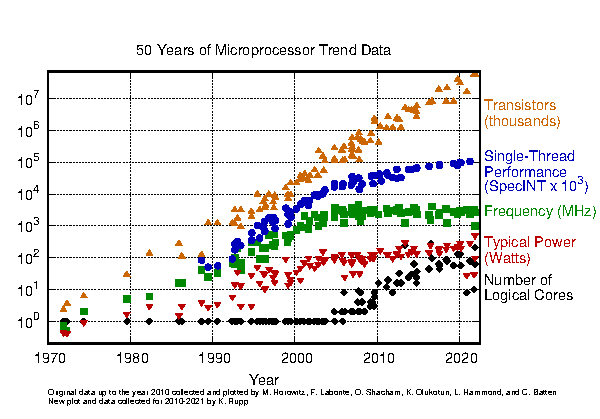
\includegraphics[width=\textwidth]{figs/50-years-processor-trend.pdf}
    \caption{近50年处理器发展趋势图}
    % \caption{近50年处理器发展趋势图\protect\footnotemark}
    \label{50yrs_processor_trend}
\end{figure}

多核架构的处理器拥有多个核心,能够同时运行多个任务,或者并行处理一个任务,大大缩短软件的运行时间。表面上看,不断增加芯片的核心数便能不断提高其处理能力,然而,多核处理器的运算能力并不能随着核数无限提升,原因如下:(1) 由于功耗墙(The power wall)的存在,即使制造出一个拥有许多个核心的芯片,也无法允许所有核心同时运行\cite{dark_silicon},这部分不工作的晶体管被称为“暗硅(Dark silicon)”;(2)在阿姆达尔定律中\cite{amdahl_law},任务在多核处理器下的理论加速比为:
\begin{equation}
    \label{amdahl_law}
    \text{加速比} = \frac{W_s+W_p}{W_s+ \frac{W_p}{p}}
\end{equation}
式中$W_s$和$W_p$为任务规模中的串行分量(不能被并行的部分)和并行分量(可以被并行的部分),可见加速比上限由任务中不能被并行处理的部分决定,若程序没有并行分量,那么不论使用多少核的处理器,任务都无法被加速;(3)由于内存提升的速度远小于处理器提升的速度,导致内存墙问题越来越严重,对某些应用来讲,盲目堆砌多核,不但不能加速任务的处理,反而导致了性能的下降\cite{multicore_bad}。

为了解决多核架构遇到的问题,软件和硬件人员分别从两方面入手进行优化。一方面,与多核处理器配套的软件如操作系统和编译器等工具开始充分发展,尽可能利用多核架构的优点,提高任务的运行速度;另一方面,计算机体系结构人员开始采用不同的方法来解决“暗硅”问题和内存墙问题。对于内存墙问题,研究人员使用多级缓存(Multi-level caches)结构和更先进的分支预测方法来增加cache的命中率;对于“暗硅”问题,学术界和工业界提出了3个方法来充分利用未工作的晶体管\cite{is_dark_silicon}:(1)低速多核。把处理器中每个核的运行频率限制在一个较低的水平,充分利用处理器的并行性,提高运算能力,例如英特尔设计的采用太阳能供电的x86多核处理器\cite{solar_x86};(2)自动超频。允许多个核心在短时间内达到很高的频率用来处理高计算量的任务,之后迅速将每个核心的频率降低来减缓发热,常用于由电池供电的对功耗有严格要求的芯片;(3)专用集成电路(Application-Specific Integrated Circuit, ASIC)。利用ASIC性能高、发热低的优点,把“暗硅”部分设计成专用加速器,将CPU和ASIC结合,提高整体的处理能力。
为了得到能效更高的处理器,设计人员往往结合多种方法进行优化,比如英特尔的睿频技术(Turbo Boost Technology)\cite{intel_turbo_boost},ARM的大小核架构(big.LITTLE)\cite{arm_big_little}等。发展到现代,广义的处理器已经不仅仅是一个只有传统运算核心的芯片,而是成为了一个包含许多专用处理单元如GPU(Graphics Processing Unit)、NPU(Neural Processing Units)、ISP(Image Signal Processor)、嵌入式FPGA(embedded Field Programmable Gate Array, eFPGA)、DSP(Digital Signal Processing)等模块的复杂异构片上系统(System on Chip, SoC)。

随着机器学习(Machine Learning, ML)的飞速发展,人工智能(Artificial Intelligence, AI)模型对算力的需求激增。在2012年之前,训练一个ML系统所需的算力大约每17到29个月翻一番\cite{AI:computing_demand_trend},增长率和摩尔定律保持一致。然而,2012年杰弗里·辛顿(Geoffrey Everest Hinton)的学生亚历克斯·克里泽夫斯基(Alex Krizhevsky)设计了AlexNet\cite{AI:AlexNet}这一8层卷积神经网络(Convolutional Neural Network, CNN),利用GPU夺得了ImageNet LSVRC(Large Scale Visual Recognition Challenge)竞赛的冠军,并大幅领先第二名10.8个百分点,掀起了CNN研究的热潮,深度学习(Deep Learning)迎来了大爆发。伴随着互联网的快速发展和全球社会数字化转型带来的海量数据,深度学习常规模型(Regular-scale Model)训练一次所需的算力大约每4-9个月翻一番\cite{AI:computing_demand_trend}。同时,随着2016年以谷歌(Google)的AlphaGo\cite{AI:AlphaGo}战胜韩国棋手李世石为代表,大规模模型(Large-Scale Model)开始引领人工智能的潮流,计算量大约每9到10个月翻一番\cite{AI:computing_demand_trend}。如此巨大的算力需求和不断改变的算法模式是传统的运算芯片所无能为力的,于是各种领域专用架构(Domain-Specific Architecture, DSA)竞相涌现,牺牲了部分的通用性,实现了高能效计算,如寒武纪的DianNao\cite{Accelerator:DianNao}、Google的TPU(Tensor Processing Unit)\cite{Accelerator:TPU}、GraphCore的IPU(Intelligence Processing Unit)\cite{Accelerator:IPU}、华为的DaVinci架构\cite{Accelerator:DaVinci}、百度的昆仑芯片\cite{Accelerator:Kunlun}等,计算机体系结构迎来了新黄金时代\cite{new_golden}。与ASIC相比,DSA的通用性更强,能够适应日新月异的AI算法。
同时,CPU、GPU和FPGA架构也不断革新,引入了各种针对ML应用的专用处理单元,如Intel至强(Xeon)处理器中的AI加速单元\cite{Accelerator:intel_xeon_4th}、英伟达(Nvidia)GPU中的张量计算核心(Tensor Core)\cite{Accelerator:nvdia_h100_tensor_core_4th}、赛灵思(Xilinx)FPGA中的AI引擎(AI Engine, AIE)\cite{Accelerator:amd_versal_AIE}。

与计算机视觉(Computer Vision, CV)领域不同,在自然语言处理(Natural Language Processing, NLP)方面,纯粹由注意力机制构成的Transformer模型\cite{AI:attention_is_all}取代了CNN,占据了主导地位。在Google提出Transformer模型一年后,大规模语言模型(Large Language Model, LLM)开始出现,以OpenAI旗下的GPT(Generative Pre-trained Transformer)为代表,LLM的大小一直在飞速增长:2018年发布的GPT-1参数量为1.17亿,数据量为5GB(Gigabyte);2019年发布的GPT-2参数量为15亿,数据量为40GB;2020年发布的GPT-3参数量为1750亿,数据量增加到45TB(Terabyte)。研究表明,Transformer类模型训练所需的运算量每2年增加750倍,远超摩尔定律的演进速率,如图\ref{AI:ai_and_compute}所示\cite{ai_and_memory_wall}。

\begin{figure}[htb]
    \centering
    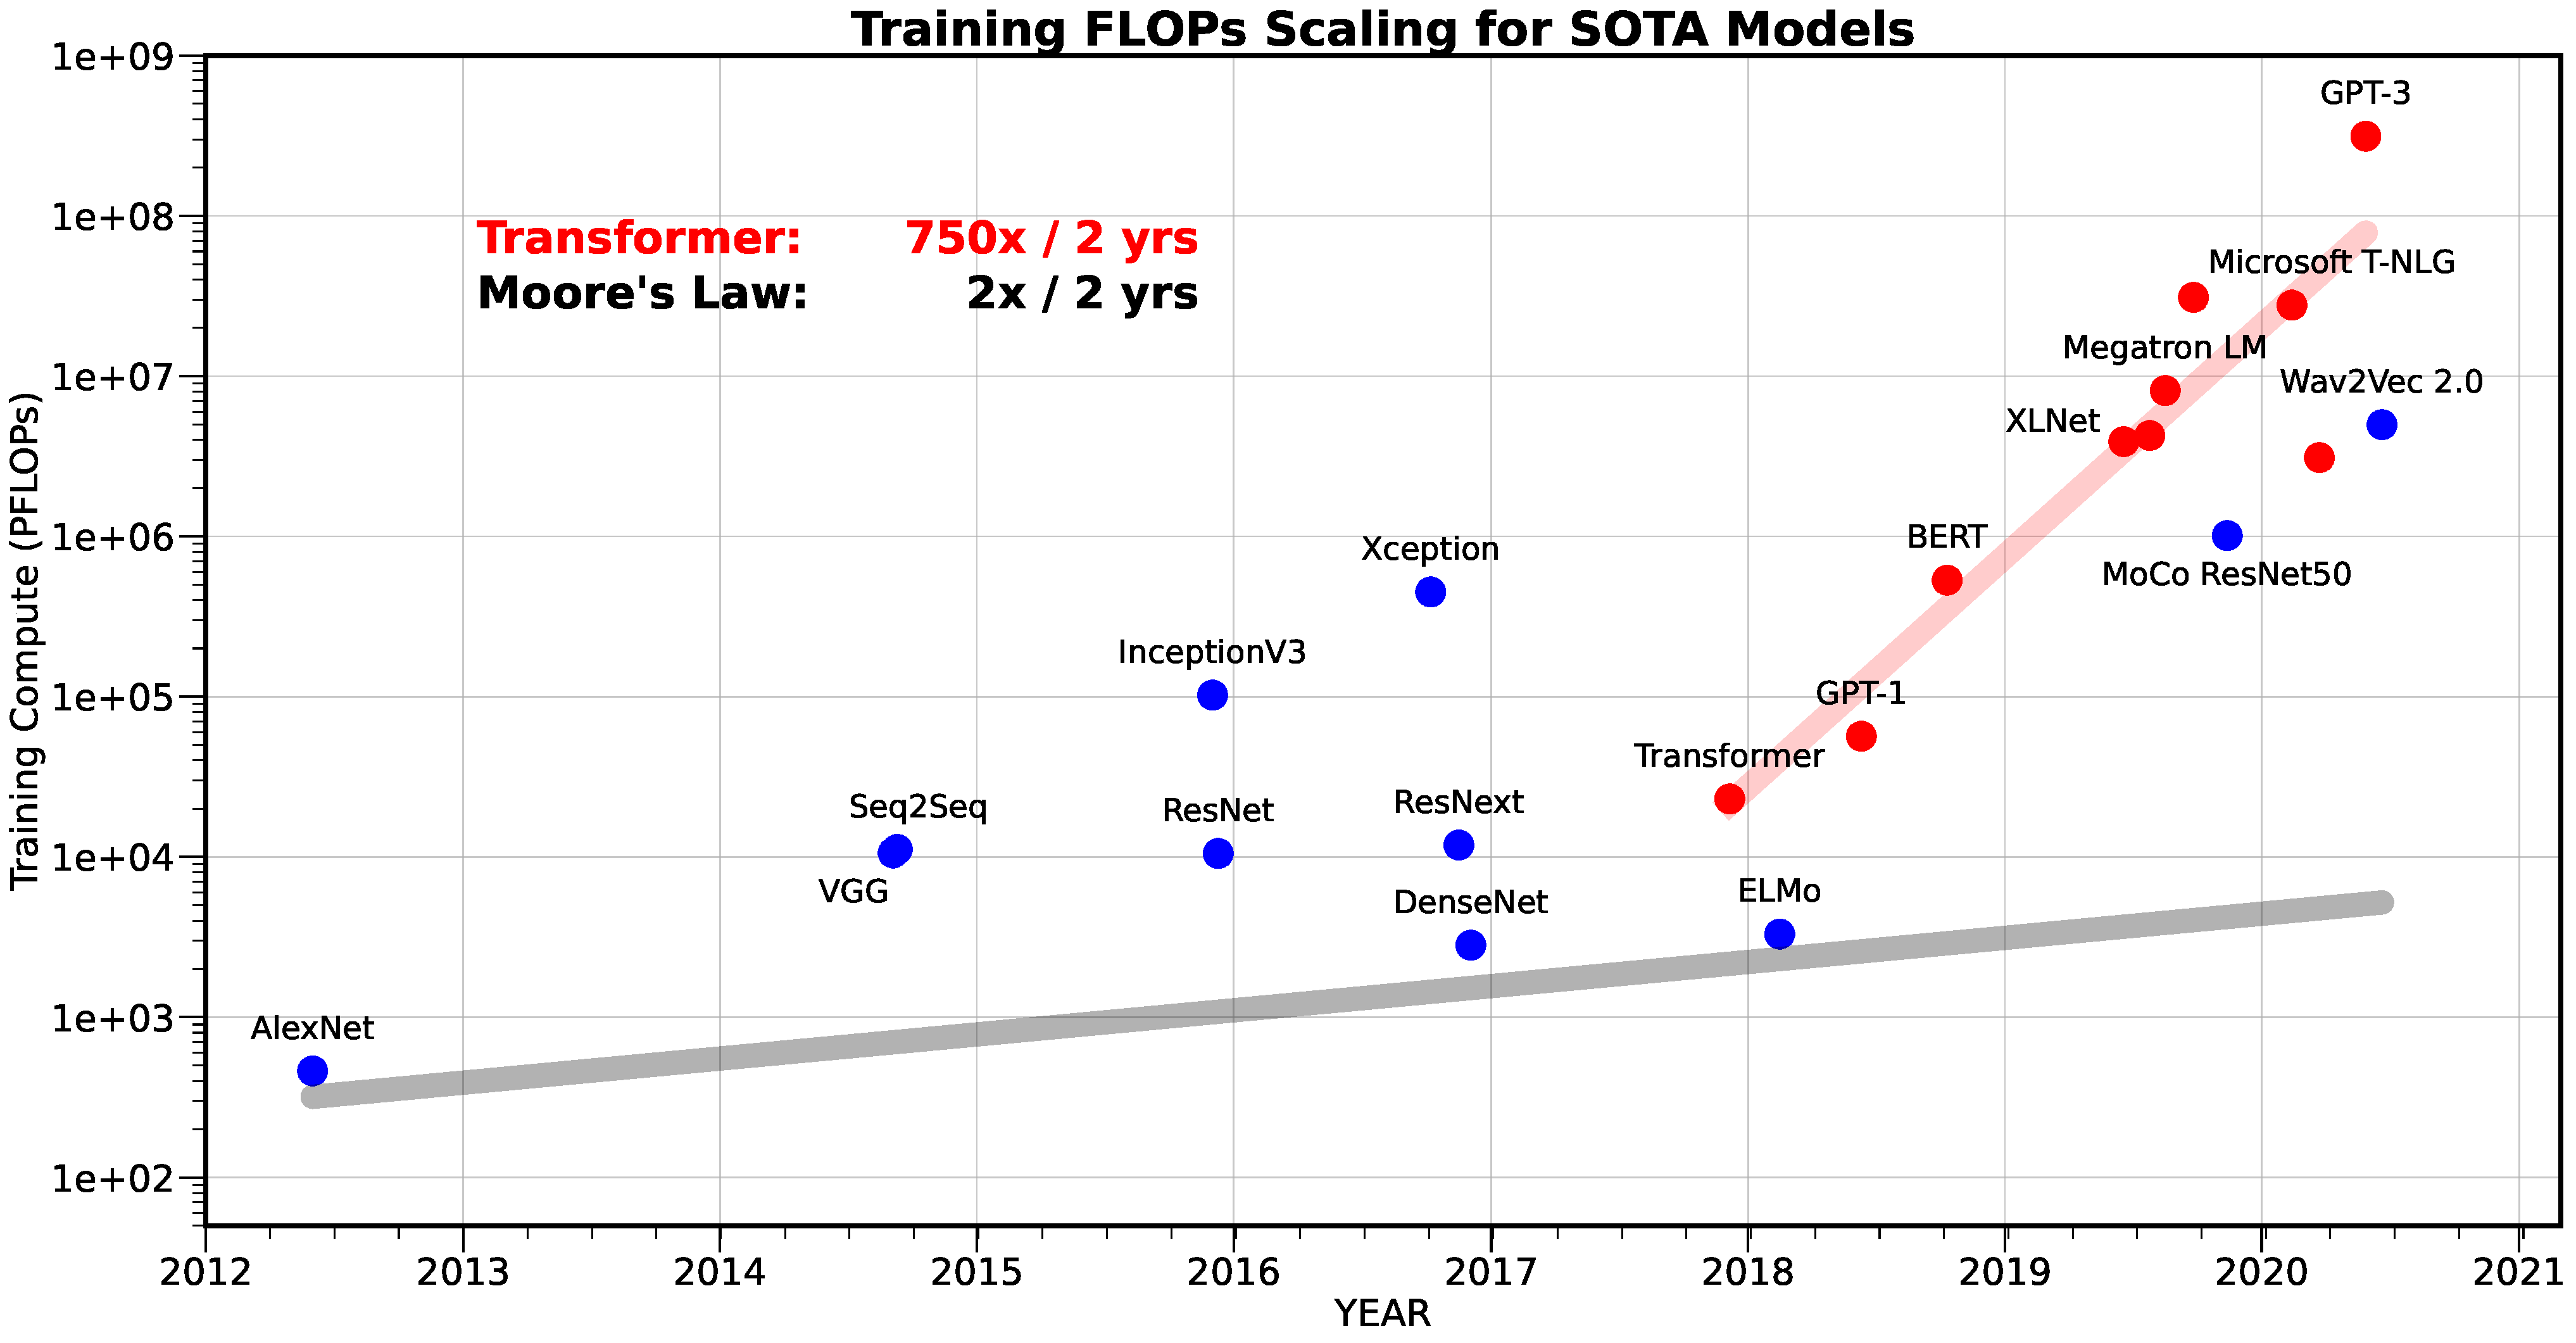
\includegraphics[width=\textwidth]{figs/AI-Fig-ai_and_compute.pdf}
    \caption{Transformer类模型训练所需的运算量}
    \label{AI:ai_and_compute}
\end{figure}


如此巨大的计算需求,需要海量的算力进行支撑。目前业界通用的办法是利用并行化技术在多个GPU或DSA上进行训练,以求在合理的时间内获得想要的结果。然而,这会伴随着资源的大量消耗。例如,训练一个GPT-3模型需要355个GPU年(一块GPU运行355年的运算量),花费460万美元,耗电1287兆瓦时(Megawatt Hour, MWh),大约相当于120个家庭1年的用电量\cite{AI:carbon_google_2021,AI:zeus}。并且,训练阶段的能耗通常只占模型整个生命周期的40\%\cite{AI:carbon_google_2022},ChatGPT的火热导致这一占比对GPT类应用更低,这产生了大量碳排放,对环境造成了很大的负担。为了降低能耗,研究人员从算法和硬件两方面来对AI应用进行优化。一方面,高效的ML模型架构可以在更少计算量的情况下实现更高的精度,减少资源的消耗;另一方面,采用专门用于AI训练和推断的芯片能够提高系统的能效,实现绿色计算(Green Computing)\cite{AI:green_computing}。但是,目前的研究表明,LLM模型的规模越大,往往NLP任务的效果越好,\cite{AI:llm_overview},这意味着模型的精简程度十分有限。同时,芯片的能效提升远远跟不上模型的规模增长,人们迫切需要新的方法在提升算力的同时降低资源消耗。


\subsection{后摩尔时代的技术路线}

以生成式AI(Generative AI)为代表的人工智能等应用的发展,对半导体材料和器件提出了更高的要求。当前,随着硅晶体管的演进接近物理极限,不仅特征尺寸的缩小越来越困难,迭代产生的工艺红利也消失殆尽,硅基电子技术临近生命周期极限。为了探索集成电路领域新的发展规律,持续提高芯片能效,学术界和工业界提出了多个发展方向,这里列举几个典型的技术路线
\ifdefined\Blind
:
\else
\footnote{https://irds.ieee.org/editions/2022}:
\fi

(1)More Moore

“More Moore”即“深度摩尔”,其基本思路是延续摩尔定律的发展,在兼顾性能和功耗的同时,继续缩小晶体管的尺寸\cite{more_moore}。随着FinFET的漏电越发严重,对沟道拥有更强控制能力的全环栅晶体管(Gate All Around FET, GAAFET)将成为未来的主流\cite{GAA}。

(2)More than Moore

“More than Moore”即“超越摩尔”,侧重于功能的多样化,由应用需求驱动,通过先进封装技术实现异质集成系统\cite{more_than_moore}。与不断优化晶体管的“More Moore”路线不同,“More than Moore”从需求端出发,以系统应用为起点,尝试在提高芯片集成度和能效的同时降低芯片制造的成本。在SoC中,除了逻辑(Logic)和存储(Dynamic Random Access Memory, DRAM)部分以外,模拟(Analog)、射频(Radio Frequency, RF)等模块往往并不能随着工艺的迭代获得显著地性能改善,甚至可能会变差。因此,数字(Digital)部分可由先进工艺实现,而其余部分可选择更合适的工艺进行流片,最后不同模块通过先进封装技术组合在一起,模块间通过高速接口进行通讯,实现整体的能效提升。


(3)Beyond Complementary Metal Oxide Semiconductor(CMOS)

前面两种路线仍然是基于硅基集成电路进行拓展,“Beyond CMOS”是指利用CMOS之外的新器件、新材料来制造晶体管,提高芯片的能效\cite{beyond_cmos}。与CMOS相比,这类新器件往往具有更高的密度、更强的性能、更低的功耗,但可能还无法大规模制造或制造成本不能接受。目前,该方向是学术界和工业界研究的热点之一,各种新型方案百花齐放,比如低功耗的隧穿场效应晶体管(Tunneling FET, TFET)\cite{TFET}、与CMOS工艺兼容的单电子晶体管(Single Electron Transistor, SET)\cite{SET}、具有高迁移率的石墨烯晶体管(Graphene Transistor)\cite{Graphene_transistor}、适合RF电路的碳纳米管场效应晶体管(Carbon Nanotube FET, CNFET)\cite{Carbon_Nanotube_FET}等。但是,这一方向的绝大多数成果还未走出实验室,仍处于初期的前瞻性研究阶段,距离商业化较远。

\subsection{近似计算的优势} \label{approximate_computing_advance}

随着人工智能的不断发展,计算需求急剧增加,带来大量的能源消耗。同时,在可穿戴设备、便携设备和数据中心等场景,集成电路面临的功耗问题同样严峻,人们需要寻找新的芯片设计方法以同时满足高性能和低功耗的严苛要求。
在实际生活中,许多应用具有错误容忍的特性,这类应用被称为容错应用(Error-tolerant applications)。一个典型的例子是,当观看视频时,由于感知的限制,即使视频中某些帧出错甚至丢失了,人类很可能也察觉不到。类似地,即使搜索引擎返回的结果没那么精确,查询者也可以接受。
近似计算(Approximate computing)是一种新型的计算范式(Paradigm),与精确计算(Exact computing)相比,它可能返回不准确的结果。与容错应用结合,近似计算可以在满足精度需求的前提下节省大量能源,达到降低功耗、提高能效的目的。
因此,在数字信号处理、机器学习等场景中,近似计算得到了工业界和学术界的广泛关注\cite{AC:survey:survey's_survey,AC:survey:hanjie_2013_ETS}。

目前,有关近似计算的研究主要集中在四个层面:

(1)软件层近似(Software-level approximation)

软件层的近似有多种实现方式,比如在循环中跳过一些迭代来更快地获得计算结果,或者根据条件语句进行判断,从而跳过某些任务的执行来减少程序运行时间。另外,许多启发式算法(Heuristic algorithm)如模拟退火(Simulated annealing)和遗传算法(Genetic algorithm)常常需要在一定的时间内获得次优解(Sub-optimal solution),也属于软件层近似的一种。

(2)近似电路(Approximate circuits):

通过对加法器(Adder)\cite{AC:Aadd:simple_yet}、乘法器(Multiplier)\cite{AC:AM:Adapt}、除法器(Divider)\cite{AC:Div:2019dac}等算术运算单元(Arithmetic units)引入近似,获得能效的提升,被称为电路级近似。电路级近似的实现方式大体上可以分为两类:电压调节(Voltage scaling)和功能近似(Functional approximation)\cite{AC:ALS:survey}。其中,电压调节是通过降低模块的工作电压但不降低频率来减少电路的功耗。然而,这一般会产生时序错误(Timing error),带来难以控制的计算误差\cite{AC:Arith:overscale}。功能近似通常聚焦在电路结构或门级网表(Gate-level netlist)的简化上,与电压调节相比,功能近似的方法带来的误差易于控制,也是目前近似计算研究最为深入的方向\cite{AC:Arith:survey_hanjie}。

(3)近似存储和近似内存(Approximate storage and memory):

与存储精确数据相比,存储近似后的数据能够改善数据读取的延迟,降低数据搬移的能耗。例如,通过舍弃浮点数(Floating-point number)低有效位(the Least Significant Bit, LSB),可以减少数据存储所需要的位宽(Bit width),提高存储密度。在基于Flash的固态硬盘(Solid State Drive, SSD)中引入近似计算可以提高SSD的读取性能\cite{AC:Store:ASCache}。对于内存或cache来说,降低DRAM的刷新率\cite{AC:Store:DRAM}或静态随机存储器(Static Random-Access Memory, SRAM)\cite{AC:Store:SRAM}的供电电压也可以达到节省功耗的目的。

(4)近似系统(Approximate system):

对不同子模块如传感器、内存、处理器、通信接口等进行协同优化的方法被称为近似系统,与单独优化各个组件相比,近似系统能够取得更好的效果\cite{AC:Sys:camera}。


% \section{国内外研究现状}


\section{本文主要工作及组织结构}

本文的工作主要集中在近似电路中定点数(Fixed-point number)乘法器的设计及应用上,包含以下三个方面的研究:(1)基于白盒优化的考虑输入分布(Input distribution)和极性(Polarity)的面向ASIC的自动化近似乘法器设计方法;(2)基于黑盒优化的面向FPGA的自动化近似乘法器设计方法;(3)基于生成的近似乘法器库进行近似逻辑综合(Approximate Logic Synthesis, ALS)\cite{AC:ALS:survey}的研究。具体工作如下:

(1)面向ASIC,提出并开源了一个白盒优化的考虑输入分布和极性的高质量自动化近似乘法器生成方法,该方法在对部分积进行累加求和之前,引入与(AND)、或(OR)、异或(XOR)和移位(Shift)操作,降低部分积的个数,实现能效的提升。具体来说,基于应用驱动,统计应用中乘法器的输入数据分布,并在考虑极性的情况下对部分积进行压缩,减轻后续的累加负担。为了能够自动化处理,将寻找较优压缩操作的问题建模成数学问题,并用 MATLAB进行求解。
基于改进的Baugh-Wooley算法\cite{EM:baugh-wooley,EM:baugh-wooley_modified_PP_reorga,EM:baugh-wooley_diff},方法经过扩展后实现了对补码有符号乘法器的支持。基于位宽为$8\times8$无符号乘法的三个不同规模的神经网络包括LeNet、AlexNet和VGG16以及位宽为$16\times16$有符号定点数乘法的有限冲击响应(Finite Impulse Response, FIR)滤波器的实验结果表明,与国际前沿工作相比,生成的近似乘法器在几乎没有精度损失的前提下,功耗延迟面积积(Product of Power, Delay, and Area, PDA)提升了26.4\%-27.1\%。

(2)面向FPGA,设计并开源了一个基于黑盒优化的近似乘法器生成器,该方法假设乘法器的部分积在生成后、累加前存在一次由半加器阵列进行的压缩操作,针对半加器,提出删减(Eliminate)、或之和(OR $Sum$)、直接进位(Direct $Cout$)、精确(Exact)四种简化方法,利用贝叶斯优化(Bayesian optimization)和详细设计的能够同时考虑硬件PPA和软件精度的目标函数($cost$ function)对半加器的优化空间进行探索,生成高质量的近似乘法器集合。与国际前沿工作中1167个近似乘法器相比,生成的乘法器综合指标平均提升28.70\%-38.47\%,且处于帕累托前沿(Pareto front)。

(3)基于前面两种自动化方法得到的ASIC和FPGA乘法器库,首先针对传统逻辑综合,提出并开源了一个基于MFFC(Maximum Fanout-Free Cone)自适应超图划分的强化学习(Reinforcement learning)逻辑优化序列探索框架。基于超过150个电路的实验结果表明,面积延迟积(Area Delay Product, ADP)比ABC\cite{LS:ABC} resyn2平均提高了5.17\%;然后将框架与近似乘法器库结合,对基于不同近似乘法器实现的DNN加速器进行了研究,结果显示近似乘法器的单独硬件成本提升与对应加速器的硬件成本提升存在一定偏差。

本文共有六个章节,各章节的组织结构安排如下:

第一章,绪论。首先介绍了自集成电路发明以来半导体工艺和计算机体系结构的发展,之后分析了近似计算结合容错应用具有的优势,引出本文的研究目的,同时简述了本文的主要工作和创新点。

第二章,乘法器概述。首先介绍了精确定点数乘法器的运算过程及不同的实现方法,以及采用Mitchell近似的对数乘法器\cite{EM:mitchell};之后阐述了目前主流的衡量近似电路(主要是算术单元)误差的指标,这些指标同样适用于近似乘法器。

第三章,ASIC近似乘法器设计。首先分析了国内外有关ASIC近似乘法器的实现方法,主要分为四大类:手工设计(Manual design)、数学转换近似(Mathematical transformation approximation)、自动化方法(Automated method)、近似电路综合(Approximate circuit synthesis);接着介绍了基于白盒优化的考虑数据分布和输入极性的自动化近似乘法器设计方法,并与国际前沿工作进行对比。

第四章,FPGA近似乘法器设计。首先介绍了学术界提出的面向FPGA领域的多种近似乘法器设计方法,主要是通过手工修改查找表(LookUp Table, LUT)编码的方式实现;接着提出了基于黑盒优化的自动化近似乘法器生成器,并与国际前沿工作进行误差和硬件开销比较。

第五章,近似逻辑综合。首先介绍了传统的逻辑综合,设计并实现了一个基于MFFC(Maximum Fanout-Free Cone)自适应超图划分的强化学习逻辑优化序列探索框架,并与已有的序列优化方法进行对比;之后与近似乘法器库结合,探究不同近似乘法器对DNN硬件加速器带来的影响。

第六章,总结与展望。该章节总结了本文的主要研究工作和成果,分析了工作中存在的局限性,并对未来进一步的探索方向进行了展望。


%   \chapter{乘法器与逻辑综合技术基础}

\section{精确乘法器} \label{精确乘法器}

% 大多数近似乘法器是基于精确乘法器优化得到的,在介绍有关近似乘法器的内容之前,对精确乘法器的不同实现方法做一个回顾是必要的。与浮点数相比,定点数消耗的存储资源更少,在硬件上更容易实现,运算效率也更高,本文的研究集中在定点数乘法器。

计算机中的数值类型分为无符号数(Unsigned number)和有符号数(Signed number),不论基于哪种数值类型设计的精确乘法器,其运算过程均可以看作以下三个步骤: 部分积的生成、部分积的累加、以及最终相加。对部分积的生成来说,与无符号数相比,采用补码表示的有符号数相乘时需要对部分积进行符号位扩展(Sign extension),并对最后一个部分积执行减法,这一方面增加了部分积的规模,不利于后续的累加操作,另一方面需要硬件支持减法,增加了设计的复杂度。
安德鲁·唐纳德·布斯(Andrew Donald Booth)于1950年提出了用于二进制补码有符号数相乘的布斯算法\cite{EM:booth_orig},该算法把符号位和数值位统一进行编码,通过移位操作跳过对乘数(Multiplier)中连续的1进行计算,提高乘法的运算速度,但在某些特殊情况下反而会增加部分积的操作次数%
\IfStrEq{\Version}{Open}{%
    \footnote{\url{https://www.quora.com/How-does-Booths-algorithm-work/answer/Raymond-Paseman}}。
}{。}
经过改进,基4的布斯编码(Radix-4 Booth encoding)在任何情况下都能将部分积的个数降低一半\cite{EM:booth_Macsorley,EM:booth_proof},提高了电路的性能,得到了广泛的应用。
Baugh和Wooley于1973年提出了Baugh-Wooley算法\cite{EM:baugh-wooley},将补码乘法中所有部分积的权重转换为正数,避免符号位扩展和减法操作,有利于硬件实现。
与生成相比,部分积的累加方式复杂,优化空间大,因此,采用不同加法结构的累加阵列如华莱士树(Wallace tree)\cite{EM:Wallace}、达达树(Dadda tree)\cite{EM:Dadda}等被广泛研究。

\subsection{部分积的生成}

\subsubsection{无符号乘法器}

一般地,一个任意的整数位宽为$n$、小数位宽为$m$的无符号$R$进制定点数($R$是正整数,$R \geq 2$):
\begin{equation}
\begin{split}
   A = a_{n-1} a_{n-2} \cdots a_1 a_0 . a_{-1} a_{-2} \cdots a_{-m+1} a_{-m}
\end{split}
\label{EM:Eq:unsigned_fixed_Binary}
\end{equation}
其十进制值为:
% \begin{equation}
\begin{align}
    % D(A_R) = \ & a_{n-1} \times R^{n-1} + a_{n-2} \times R^{n-2} + \cdots + a_1 \times R^1 + a_0 \times R^0 + \notag \\
    % & a_{-1} \times R^{-1} + a_{-2} \times R^{-2} + \cdots + a_{-m+1} \times R^{-m+1} + a_{-m} \times R^{-m} \notag \\
    % = & \sum_{i=-m}^{n-1} a_i \times R^i \ge 0
    V(A) = \ & a_{n-1}  R^{n-1} + a_{n-2}  R^{n-2} + \cdots + a_1  R^1 + a_0  R^0 + \notag \\
    & a_{-1}  R^{-1} + a_{-2}  R^{-2} + \cdots + a_{-m+1}  R^{-m+1} + a_{-m}  R^{-m} \notag \\
    = & \sum_{i=-m}^{n-1} a_i  R^i \ge 0
\label{EM:Eq:unsigned_fixed_Decimal}
\end{align}
% \end{equation}
其中$R$被称为基数,$R=2$时表示二进制;$a_i$是自然数且$a_i \in [0,R-1]$;$n,m$是自然数,$n+m \ge 1$,$n=0$和$m=0$时分别表示无符号纯小数和无符号整数。

计算机采用二进制进行计数,无符号二进制乘法器(Unsigned binary multiplier)是用来计算两个非负二进制定点数(0及正数)乘积的运算器件,部分积是通过被乘数(Multiplicand)和乘数(Multiplier)的逻辑与(AND)得到的,每个部分积的权重不同,图\ref{EM:Fig:unsigned_mul_PP_gen}展示了两个无符号二进制整数($6\times5$)的运算过程,共有三个部分积110、000、110,权重依次为$2^0$、$2^1$、$2^2$,X表示0。计算定点数时,由于硬件上并不存在小数点的概念,因此将数字视为整数直接相乘,最后计算缩放倍数。
\begin{figure}[!htb]
    \centering
    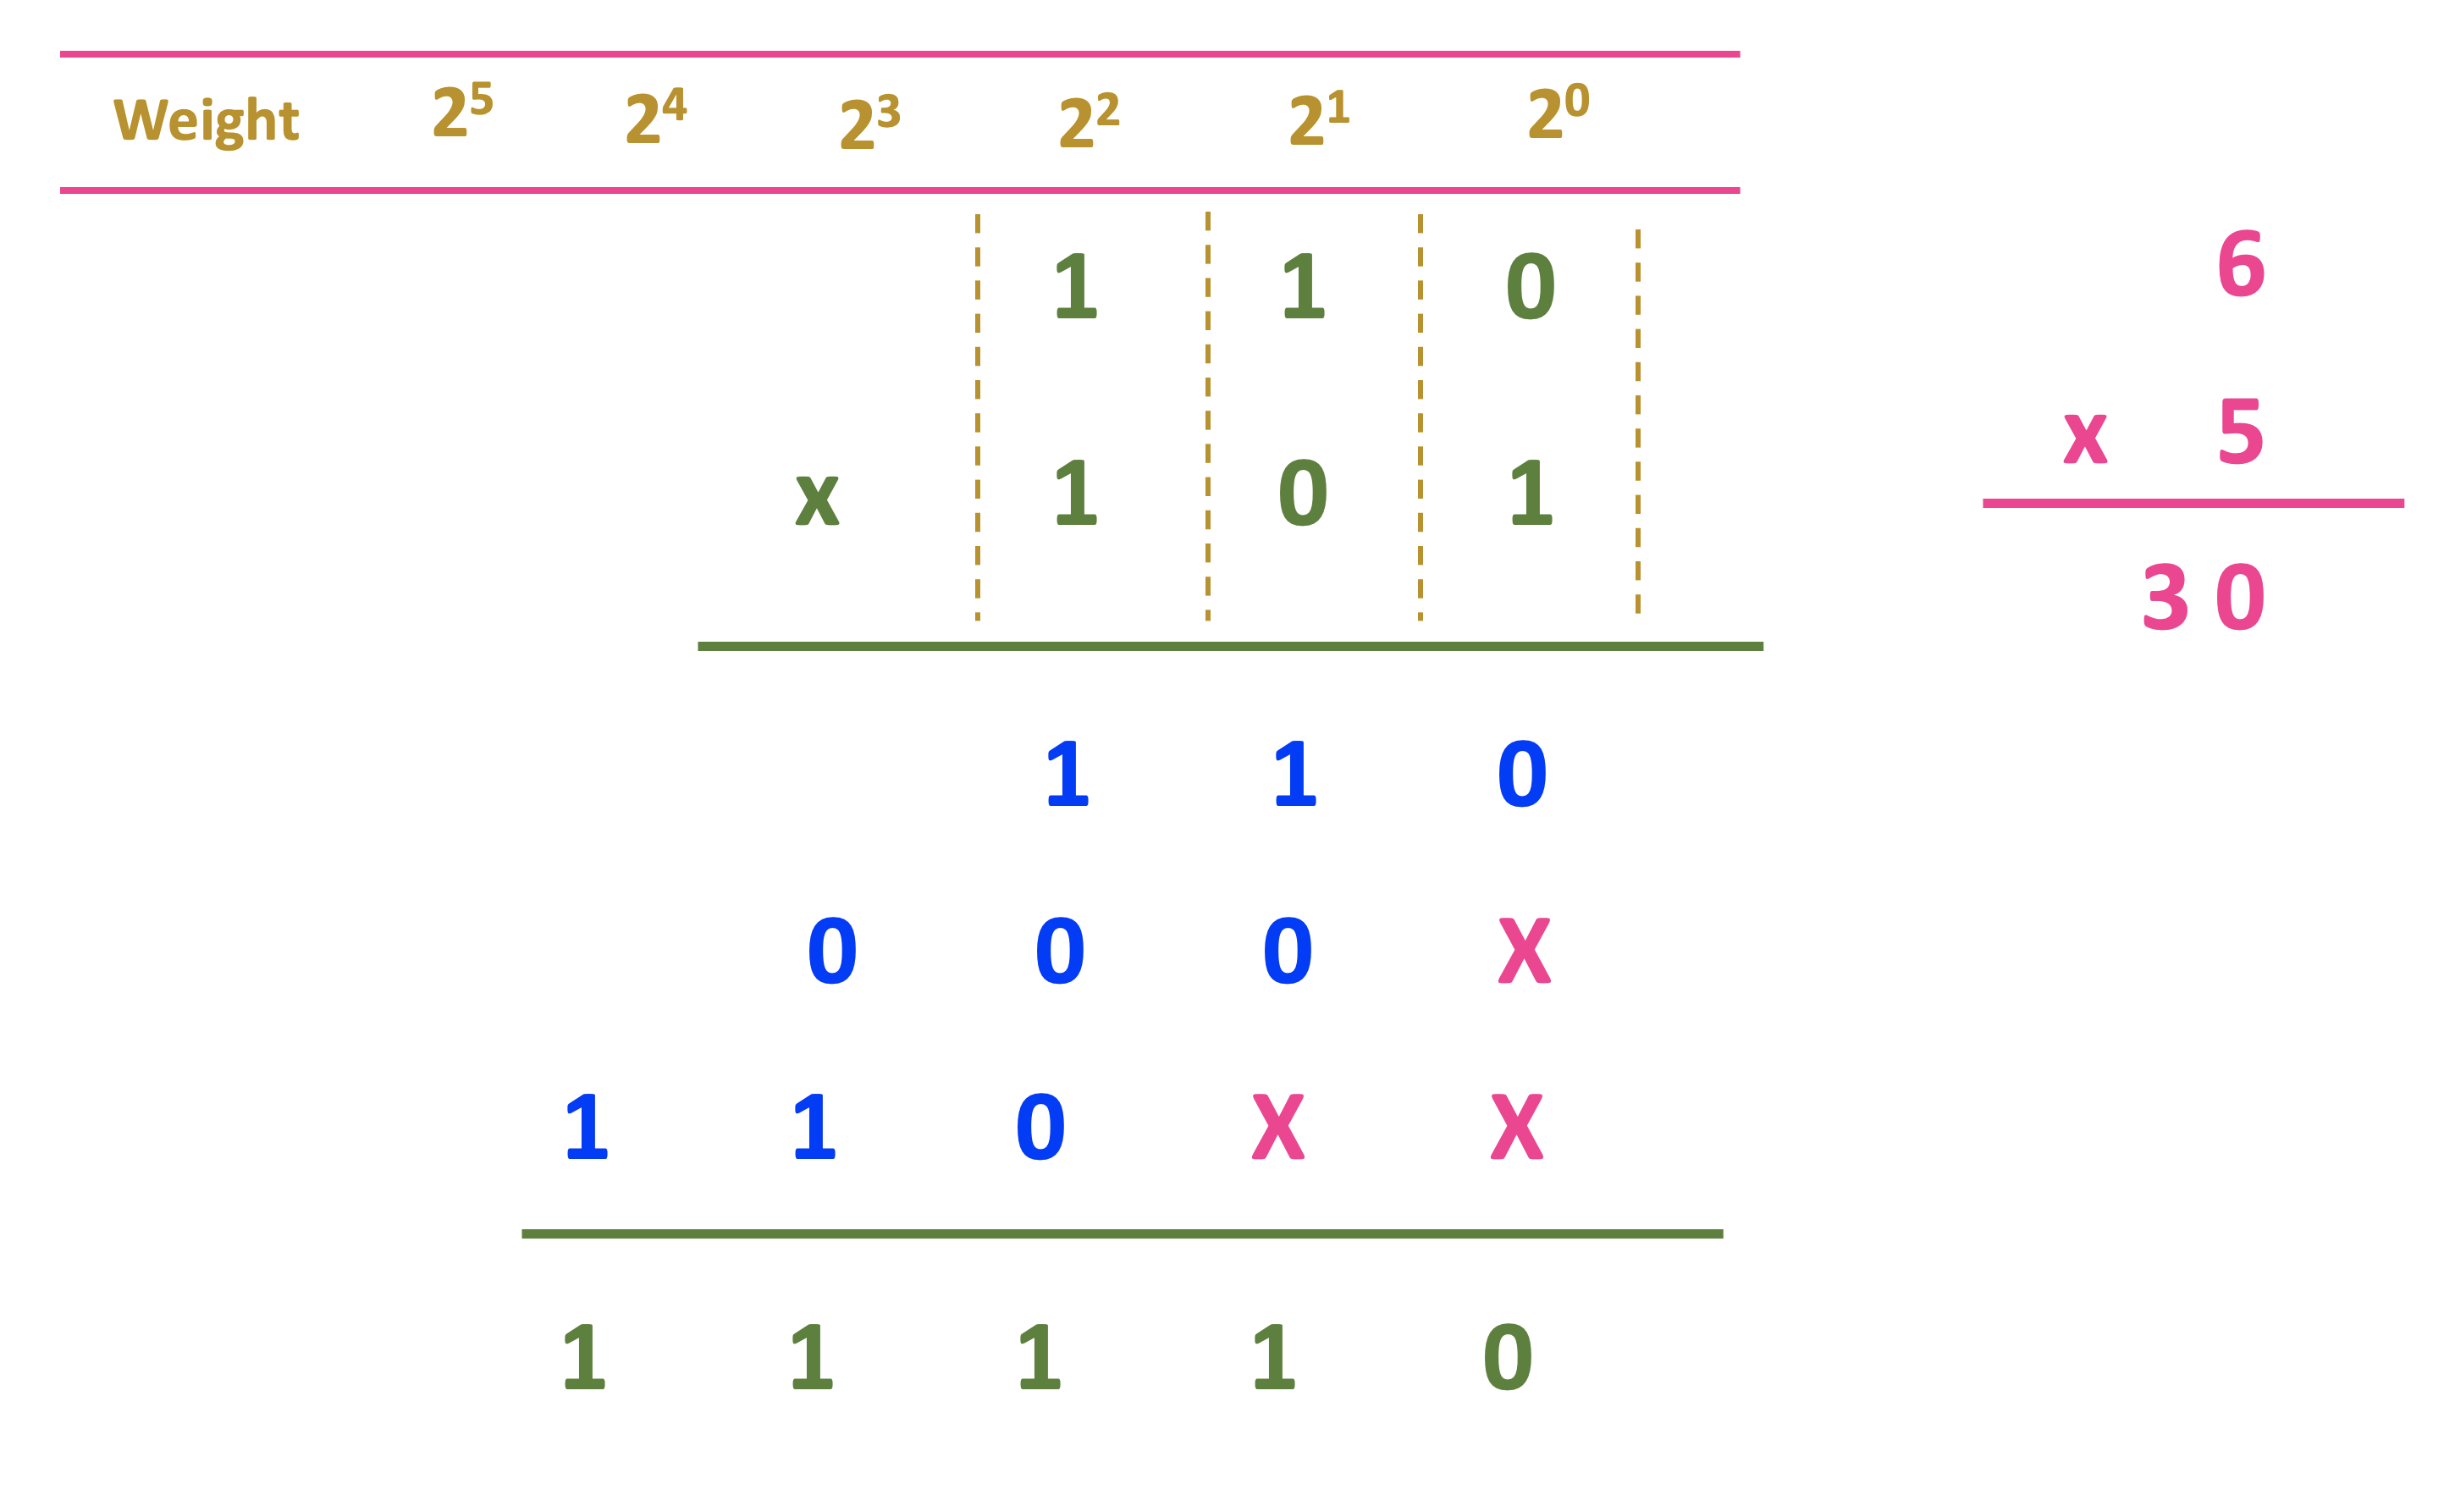
\includegraphics[width=0.8\textwidth]{figs/EM-Fig-unsigned_mul_PP.png}
    \caption{两个无符号整数的运算过程}
    \label{EM:Fig:unsigned_mul_PP_gen}
\end{figure}




\subsubsection{补码有符号乘法器}

无符号数不能表示负数,为了解决二进制下的问题,研究人员引入了原码(True form)、反码(1's complement)和补码(2's complement)来表示数据。
与无符号数相比,原码在最高位额外增加了一位符号位用来区分正负,0表示正数,1表示负数;在反码中,正数的反码就是其原码,负数的反码是将原码中,除符号位外,每一位按位取反;在补码中,正数的补码同样是其原码,负数的补码是其反码加一。
与原码和反码相比,补码避免了加减法不统一和存在两个零值的缺点,简化了硬件电路设计的复杂度,因此现代计算机底层采用补码的编码方式对数据进行存储和运算。
若式\eqref{EM:Eq:unsigned_fixed_Binary}为补码,$R=2$时,其最高位权重为$-2^{n-1}$,式\eqref{EM:Eq:unsigned_fixed_Decimal}变为:
% \begin{equation}
\begin{align}
    % V(A) = & \ D(A_2) \notag \\
    % = & \ ( \ \textcolor{red}{-}a_{n-1} \times R^{n-1} + a_{n-2} \times R^{n-2} + \cdots + a_1 \times R^1 + a_0 \times R^0 + \notag \\
    % & \ a_{-1} \times R^{-1} + a_{-2} \times R^{-2} + \cdots + a_{-m+1} \times R^{-m+1} + a_{-m} \times R^{-m} \ )_{10} \notag \\
    % = & \  ( \ \textcolor{red}{-}a_{n-1} \times 2^{n-1} + a_{n-2} \times 2^{n-2} + \cdots + a_1 \times 2^1 + a_0 \times 2^0 + \label{EM:Eq:signed_fixed_Decimal} \\
    % & \ a_{-1} \times 2^{-1} + a_{-2} \times 2^{-2} + \cdots + a_{-m+1} \times 2^{-m+1} + a_{-m} \times 2^{-m} \ )_{10} \notag \\
    % = & \ ( \textcolor{red}{-}a_{n-1} \times 2^{n-1} + \sum_{i=-m}^{n-2} a_i \times 2^i \ )_{10} \notag
    V(A) = & \ \textcolor{red}{-}a_{n-1}  R^{n-1} + a_{n-2}  R^{n-2} + \cdots + a_1  R^1 + a_0  R^0 + \notag \\
    & \ a_{-1}  R^{-1} + a_{-2}  R^{-2} + \cdots + a_{-m+1}  R^{-m+1} + a_{-m}  R^{-m} \notag \\
    = & \ \textcolor{red}{-}a_{n-1}  2^{n-1} + a_{n-2}  2^{n-2} + \cdots + a_1  2^1 + a_0  2^0 + \notag \\
    & \ a_{-1}  2^{-1} + a_{-2}  2^{-2} + \cdots + a_{-m+1}  2^{-m+1} + a_{-m}  2^{-m} \notag \\
    = & \ \textcolor{red}{-}a_{n-1}  2^{n-1} + \sum_{i=-m}^{n-2} a_i  2^i
\label{EM:Eq:signed_fixed_Decimal}
\end{align}
% \end{equation}

这里$n+m \ge 2$(引入了一位符号位),$n=1$和$m=0$时分别表示补码纯小数和补码整数。若不局限于二进制,式\eqref{EM:Eq:signed_fixed_Decimal}不一定成立%
\IfStrEq{\Version}{Open}{%
    \footnote{\url{https://blog.csdn.net/mydreamongo/article/details/8863502}},
}{,}
即任意$R$进制下,补码的最高位权重不一定是$-R^{n-1}$。
另外,一般地,对一个$N$位二进制定点数,忽略小数点,不同编码方式能够表示的数值范围为:
% \begin{equation}
% \begin{align}
%     & \text{无符号数:}  & [0, \ R^N-1] \ , \\
%     & \text{原码与反码:}  & [- \lfloor \frac{R^N-1}{2} \rfloor, \ \lfloor \frac{R^N-1}{2} \rfloor] \ , \\
%     & \text{补码:} & [- \lceil \frac{R^N-1}{2} \rceil, \ \lfloor \frac{R^N-1}{2} \rfloor] \ .
% \end{align}
% \end{equation}
\begin{align}
    & \text{无符号数:}  & [0, \ 2^N-1] \ , \\
    & \text{原码与反码:}  & [- \lfloor \frac{2^N-1}{2} \rfloor, \ \lfloor \frac{2^N-1}{2} \rfloor] \ , \\
    & \text{补码:} & [- \lceil \frac{2^N-1}{2} \rceil, \ \lfloor \frac{2^N-1}{2} \rfloor] \ .
\end{align}
式中$\lfloor \ \rfloor$和$\lceil \ \rceil$分别表示向下取整和向上取整。例如,$N=8$时,原码和反码的表示范围为[-127,127],补码的表示范围为[-128,127]。
% $R=3$,$N=4$时,原码、反码和补码的表示范围均为[-40,40]。
% \textcolor{red}{之后的内容,只要不特殊说明,均基于二进制($R=2$)。}

对于补码有符号二进制乘法器(Signed binary multiplier),目前常见的部分积生成方法有:符号位扩展、改进的Baugh–Wooley算法\cite{EM:baugh-wooley,EM:baugh-wooley_modified_PP_reorga,EM:baugh-wooley_diff}、以及基4的布斯编码\cite{EM:booth_orig,EM:booth_Macsorley,EM:booth_proof}。下面分别进行介绍:

(1)符号位扩展。

按照实现细节分类,符号位扩展方法分为两种:一种是操作数(Operand)符号位扩展,优点是硬件不需要支持减法,缺点是部分积的规模巨大,累加电路非常复杂;第二种是部分积符号位扩展,优点是不需要修改操作数,部分积的规模适中,缺点是需要对最后一个部分积执行减法。具体细节如下:
\begin{itemize}
    \item 操作数符号位扩展:首先根据乘数和被乘数确定乘积的位宽,然后将两个操作数的位宽扩展到乘积位宽,扩展方法为高位符号位扩展,即正数进行0扩展,负数进行1扩展;之后仿照无符号数二进制乘法通过逻辑与(AND)得到部分积;最后进行累加求和,注意求和后的结果应根据乘积的正确位宽进行截断。
    \item 部分积符号位扩展:同样先确定乘积所需要的位宽,不修改操作数,通过逻辑与(AND)得到部分积;然后对部分积进行高位符号位扩展(正数0扩展,负数1扩展),将每个部分积的位宽扩展到乘积位宽;最后对部分积进行累加,但对最后一个部分积执行减法。注意对于二进制补码来说, $-[A]_\text{补} = [-A]_\text{补}$,即可以通过“按位取反加1,符号位进位舍弃”的方法得到一个补码的相反数,将减法转换为加法。
\end{itemize}
% \begin{figure}[!htb]
%     \centering
%     \subfigure[操作数符号位扩展示意图。]{
%     \label{EM:Fig:操作数符号位扩展}
%     \begin{minipage}[t]{0.54\linewidth}
%     \centering
%     \includegraphics[width=\linewidth]{figs/EM:Fig:操作数符号位扩展.pdf}
%     \end{minipage}
%     }\ \ \ 
%     \subfigure[部分积符号位扩展示意图。]{
%     \label{EM:Fig:部分积符号位扩展}
%     \begin{minipage}[t]{0.4\linewidth}
%     \centering
%     \includegraphics[width=\linewidth]{figs/EM:Fig:部分积符号位扩展.pdf}
%     \end{minipage}
%     }
% \caption{补码乘法器的两种符号位扩展方法示意图}
% \label{EM:Fig:signed_mul_sign_extension}
% \end{figure}
\begin{figure}[!htb]
    \centering
    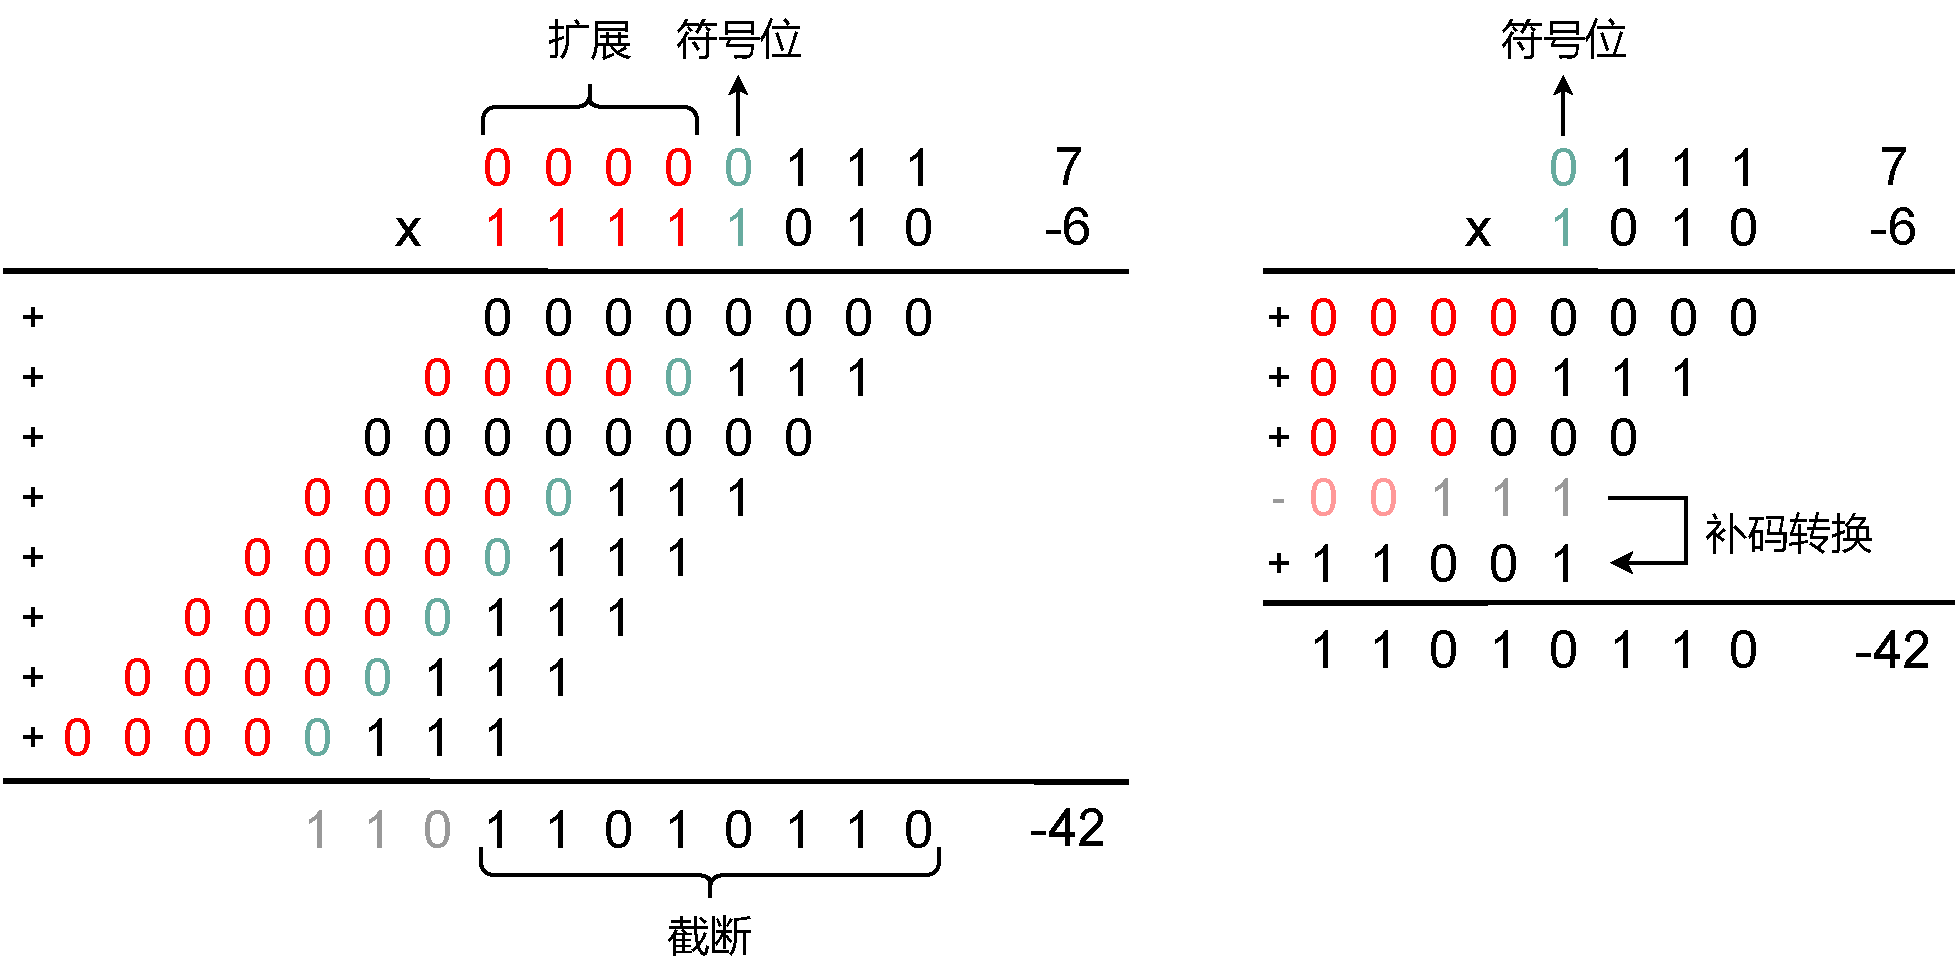
\includegraphics[width=\textwidth]{figs/EM-Fig-符号位扩展.pdf}
    \caption{补码乘法器的符号位扩展示例:左:操作数符号位扩展,右:部分积符号位扩展。}
    \label{EM:Fig:signed_mul_sign_extension}
\end{figure}

图\ref{EM:Fig:signed_mul_sign_extension}举例说明了两种符号位扩展方法的不同之处。可以看到,与操作数扩展相比,部分积扩展需要的加法更少,对应的硬件实现也更具有优势。然而,与无符号乘法相比,符号位扩展总会增大部分积的规模,使电路设计更复杂。有没有办法能够将其降低到和无符号乘法同一个水平?改进的Baugh-Wooley算法是一种解决方案\cite{EM:baugh-wooley,EM:baugh-wooley_modified_PP_reorga,EM:baugh-wooley_diff}。

(2)改进的Baugh-Wooley算法 \label{改进的Baugh-Wooley算法}

Baugh-Wooley算法是由Baugh和Wooley于1973年提出的用于二进制补码相乘的算法\cite{EM:baugh-wooley},该算法对权重为负的部分积进行修正,避免了符号位扩展,原理如下:

\noindent 设$m=0$,由式\eqref{EM:Eq:signed_fixed_Decimal}得两个$n$比特整数$X = x_{n-1} x_{n-2} \cdots x_1 x_0$和$Y = y_{n-1} y_{n-2} \cdots y_1 y_0$的十进制值:
\begin{equation}
    V(X) = -x_{n-1} 2^{n-1} + \sum_{i=0}^{n-2} x_i 2^i \ \ \ \ \ \ \ \
    V(Y) = -y_{n-1} 2^{n-1} + \sum_{i=0}^{n-2} y_i 2^i
\label{EM:Eq:signed_comp_XY}
\end{equation}
其乘积$P$:
% \begin{equation}
\begin{align}
    V(P) = & \ V(X)V(Y) \notag \\
    = & \ ( \textcolor{red}{-x_{n-1}  2^{n-1}} + \textcolor{magenta}{\sum_{i=0}^{n-2} x_i  2^i} ) \times
    ( \textcolor{blue}{-y_{n-1}  2^{n-1}} + \textcolor{cyan}{\sum_{i=0}^{n-2} y_i  2^i} ) \notag \\
%
    = & \ \textcolor{red}{x_{n-1}} \textcolor{blue}{y_{n-1}}  2^{2n-2} +
    \textcolor{magenta}{\sum_{i=0}^{n-2} x_i 2^i} \textcolor{cyan}{\sum_{j=0}^{n-2} y_j 2^j}
    \textcolor{red}{-x_{n-1}  2^{n-1}} \textcolor{cyan}{\sum_{i=0}^{n-2} y_i  2^i}
    \textcolor{blue}{-y_{n-1}  2^{n-1}} \textcolor{magenta}{\sum_{i=0}^{n-2} x_i  2^i} \notag \\
%
    = & \ \textcolor{red}{x_{n-1}} \textcolor{blue}{y_{n-1}}  2^{2n-2} +
    \textcolor{magenta}{\sum_{i=0}^{n-2}} \textcolor{cyan}{\sum_{j=0}^{n-2}} \textcolor{magenta}{x_i} \textcolor{cyan}{y_j} 2^{\textcolor{magenta}{i}+\textcolor{cyan}{j}} 
    \textcolor{red}{-2^{n-1}} \textcolor{cyan}{\sum_{i=0}^{n-2}} \textcolor{red}{x_{n-1}} \textcolor{cyan}{y_i 2^i}
    \textcolor{blue}{-2^{n-1}} \textcolor{magenta}{\sum_{i=0}^{n-2}} \textcolor{blue}{y_{n-1}} \textcolor{magenta}{x_i 2^i}
\label{EM:Eq:signed_comp_P}
\end{align}
% \end{equation}
$n=5$时,式\eqref{EM:Eq:signed_comp_P}对应的部分积阵列如图\ref{EM:Fig:signed_mul_PP_array}所示,其中红色部分积的权重为负数,对应式\eqref{EM:Eq:signed_comp_P}中结果的后两项:
\begin{figure}[!htb]
    \centering
    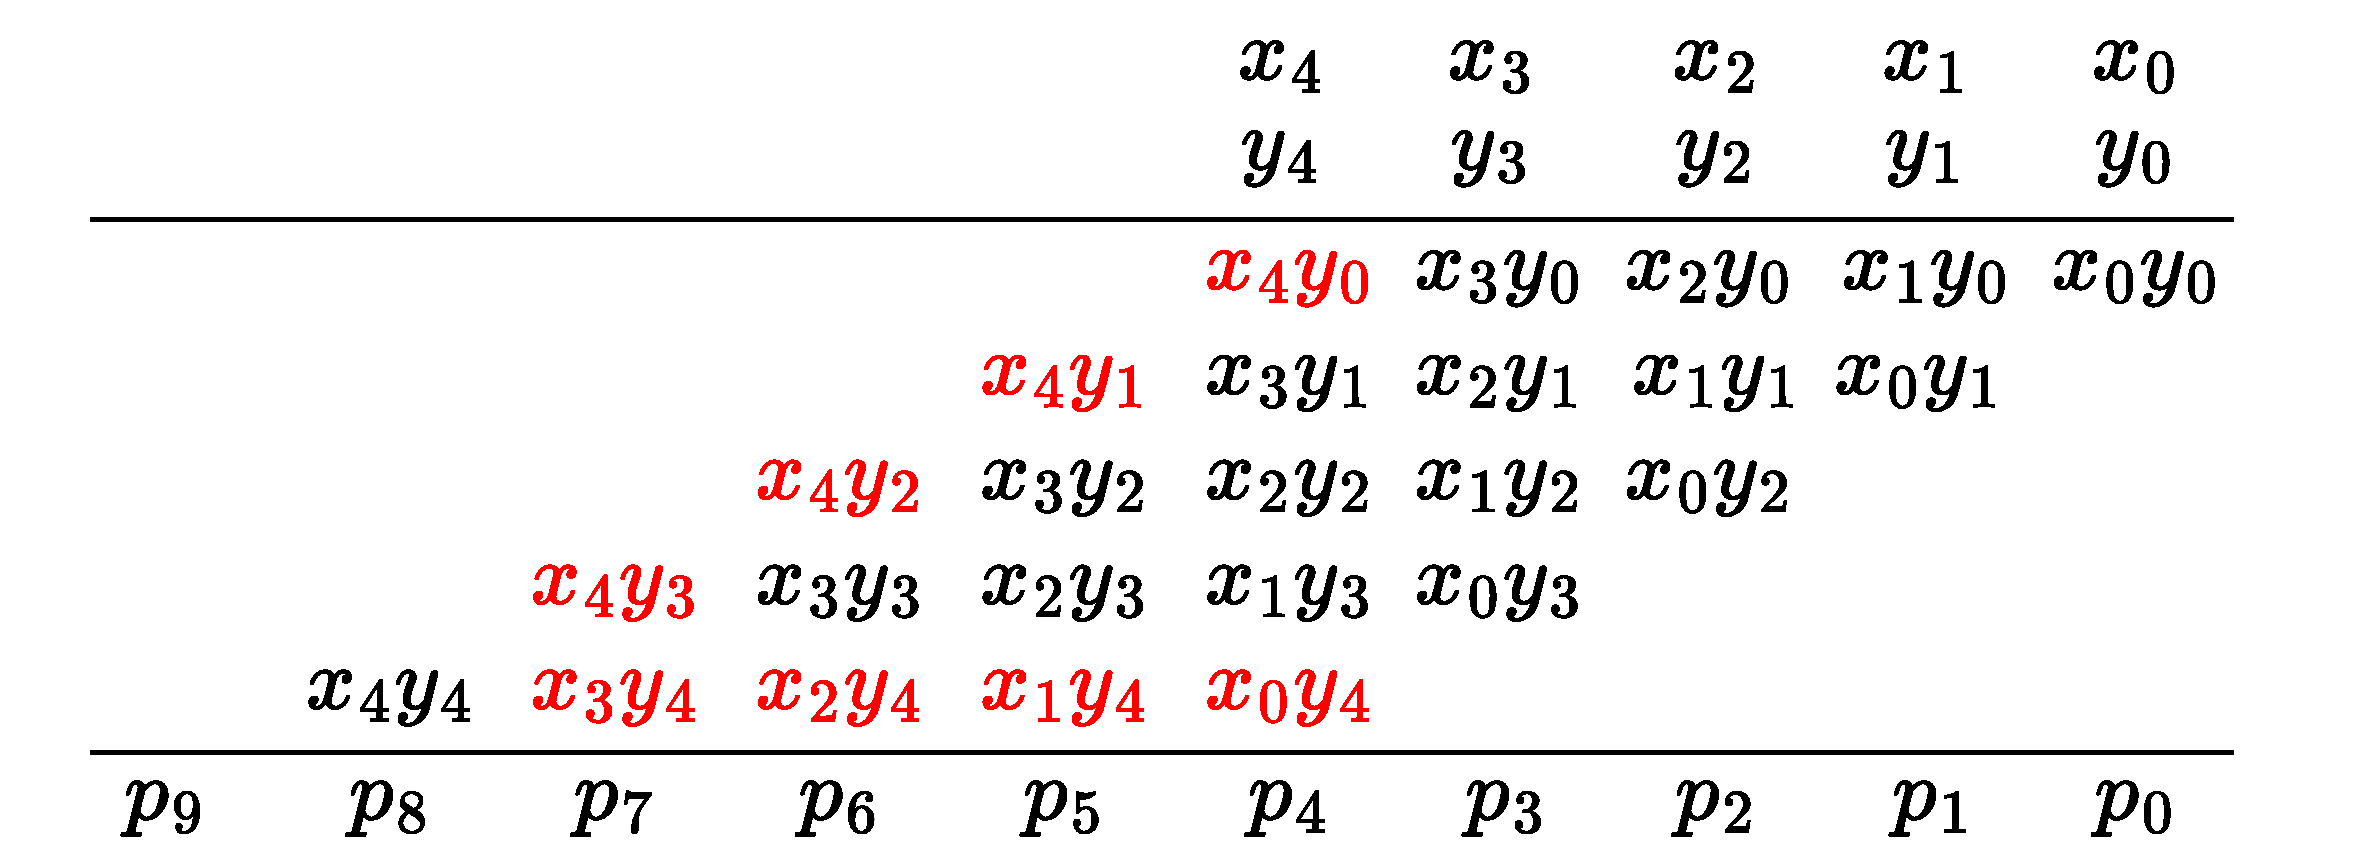
\includegraphics[width=0.85\textwidth]{figs/EM-Fig-补码部分积阵列.pdf}
    \caption{$5 \times 5$补码乘法器的部分积阵列示意图,红色部分积的权重为负}
    \label{EM:Fig:signed_mul_PP_array}
\end{figure}

\noindent 对于任意补码(不失一般性,假设是式\eqref{EM:Eq:signed_comp_XY}中的$X$):
\begin{equation}
    -V(X) = - \overline {x_{n-1}} 2^{n-1} + \sum_{i=0}^{n-2} \overline{x_i} 2^i +1 \ \ \text{(按位取反加1,符号位进位丢弃)}
    \label{EM:Eq:signed_comp_subtract}
\end{equation}
则式\eqref{EM:Eq:signed_comp_P}中结果的后两项变为:
% \begin{equation}
\begin{align}
& \textcolor{red}{-2^{n-1}} ( -0 \cdot 2^n + 0 \cdot 2^{n-1} + \textcolor{cyan}{\sum_{i=0}^{n-2}} \textcolor{red}{x_{n-1}} \textcolor{cyan}{y_i 2^i} )
\textcolor{blue}{-2^{n-1}} ( -0 \cdot 2^n + 0 \cdot 2^{n-1} + \textcolor{magenta}{\sum_{i=0}^{n-2}} \textcolor{blue}{y_{n-1}} \textcolor{magenta}{x_i 2^i} ) \notag \\
%
= & \textcolor{red}{+2^{n-1}} ( -1 \cdot 2^n + 1 \cdot 2^{n-1} + \textcolor{cyan}{\sum_{i=0}^{n-2}} \overline{ \textcolor{red}{x_{n-1}}  \textcolor{cyan}{y_i}}  \textcolor{cyan}{2^i} + 1 ) \
\textcolor{blue}{+2^{n-1}} ( -1 \cdot 2^n + 1 \cdot 2^{n-1} + \textcolor{magenta}{\sum_{i=0}^{n-2}} \overline{ \textcolor{blue}{y_{n-1}}  \textcolor{magenta}{x_i} } \textcolor{magenta}{2^i} + 1 ) \label{EM:Eq:signed_comp_P_Baugh-Wooley_positve}
\end{align}

\noindent 为了避免出现与非门(NAND),注意到式\eqref{EM:Eq:signed_comp_P_Baugh-Wooley_positve}中结果的第一项为:
\begin{equation}
    \left\{
    \begin{aligned}
        \ & 0 , & \ \ x_{n-1} = 0, \\
        \ & \textcolor{red}{+2^{n-1}} ( - 2^n + 2^{n-1} + \textcolor{cyan}{\sum_{i=0}^{n-2}} \overline{ \textcolor{cyan}{y_i}}  \textcolor{cyan}{2^i} + 1 ), & \ \ x_{n-1} = 1.
    \end{aligned}
    \right.
\end{equation}
即:
\begin{equation}
    \textcolor{red}{+2^{n-1}} ( - 2^n + 2^{n-1} + \overline{x_{n-1}} 2^{n-1} + x_{n-1} + \textcolor{cyan}{\sum_{i=0}^{n-2}} x_{n-1} \overline{ \textcolor{cyan}{y_i}}  \textcolor{cyan}{2^i} )
\label{EM:Eq:signed_comp_P_Baugh-Wooley_rNAND_x}
\end{equation}
同理第二项为:
\begin{equation}
    \left\{
    \begin{aligned}
        \ & 0 , & \ \ y_{n-1} = 0, \\
        \ & \textcolor{blue}{+2^{n-1}} ( - 2^n + 2^{n-1} + \textcolor{magenta}{\sum_{i=0}^{n-2}} \overline{ \textcolor{magenta}{x_i} } \textcolor{magenta}{2^i} + 1 ), & \ \ y_{n-1} = 1.
    \end{aligned}
    \right.
\end{equation}
即:
\begin{equation}
    \textcolor{blue}{+2^{n-1}} ( - 2^n + 2^{n-1} + \overline{y_{n-1}} 2^{n-1} + y_{n-1} + \textcolor{magenta}{\sum_{i=0}^{n-2}} y_{n-1} \overline{ \textcolor{magenta}{x_i} } \textcolor{magenta}{2^i} )
\label{EM:Eq:signed_comp_P_Baugh-Wooley_rNAND_y}
\end{equation}
结合式\eqref{EM:Eq:signed_comp_P}、式\eqref{EM:Eq:signed_comp_P_Baugh-Wooley_positve}、式\eqref{EM:Eq:signed_comp_P_Baugh-Wooley_rNAND_x}和式\eqref{EM:Eq:signed_comp_P_Baugh-Wooley_rNAND_y},$V(P)$变为:
\begin{equation}
\begin{aligned}
    V(P) = & \ \textcolor{red}{x_{n-1}} \textcolor{blue}{y_{n-1}}  2^{2n-2} +
    \textcolor{magenta}{\sum_{i=0}^{n-2}} \textcolor{cyan}{\sum_{j=0}^{n-2}} \textcolor{magenta}{x_i} \textcolor{cyan}{y_j} 2^{\textcolor{magenta}{i}+\textcolor{cyan}{j}} \\
%
    & \ \textcolor{red}{+2^{n-1}} ( - 2^n + 2^{n-1} + \overline{x_{n-1}} 2^{n-1} + x_{n-1} + \textcolor{cyan}{\sum_{i=0}^{n-2}} x_{n-1} \overline{ \textcolor{cyan}{y_i}}  \textcolor{cyan}{2^i} ) \\
%
    & \ \textcolor{blue}{+2^{n-1}} ( - 2^n + 2^{n-1} + \overline{y_{n-1}} 2^{n-1} + y_{n-1} + \textcolor{magenta}{\sum_{i=0}^{n-2}} y_{n-1} \overline{ \textcolor{magenta}{x_i} } \textcolor{magenta}{2^i} )
\end{aligned}
\label{EM:Eq:signed_comp_P_Baugh-Wooley}
\end{equation}
式\eqref{EM:Eq:signed_comp_P_Baugh-Wooley}被称为Baugh-Wooley算法,$n=5$时,该算法对应的部分积阵列如图\ref{EM:Fig:orig_Baugh-Wooley_PP}所示,所有比特权重均为正值(除了最高位的1)。与同位宽的无符号乘法器相比,不论$n$多大,由式\eqref{EM:Eq:signed_comp_P_Baugh-Wooley}得到的部分积阵列只会增加5个比特,大大优于符号位扩展方法。然而,原始的Baugh-Wooley方法会导致部分积阵列增加两层(如图\ref{EM:Fig:orig_Baugh-Wooley_PP}中的$x_4$与$y_4$),不利于后续的累加操作,注意到式\eqref{EM:Eq:signed_comp_P_Baugh-Wooley_positve}可变为:
\begin{equation}
\textcolor{red}{+2^{n-1}}  \textcolor{cyan}{\sum_{i=0}^{n-2}} \overline{ \textcolor{red}{x_{n-1}}  \textcolor{cyan}{y_i}}  \textcolor{cyan}{2^i}
\textcolor{blue}{+2^{n-1}} \textcolor{magenta}{\sum_{i=0}^{n-2}} \overline{ \textcolor{blue}{y_{n-1}}  \textcolor{magenta}{x_i} } \textcolor{magenta}{2^i} + 1 \cdot 2^n -1 \cdot 2^{2n-1}
\label{EM:Eq:signed_comp_P_Baugh-Wooley_modified}
\end{equation}
Hatamian等人根据式\eqref{EM:Eq:signed_comp_P_Baugh-Wooley_modified}对部分积进行了重新排列\cite{EM:baugh-wooley_modified_PP_reorga},得到了\ref{EM:Fig:modified_Baugh-Wooley_PP},被称为改进的Baugh-Wooley算法%
\IfStrEq{\Version}{Open}{%
    \footnote{\url{https://zhuanlan.zhihu.com/p/343133392}},
}{,}
只对部分积引入两个1,不增加部分积阵列的层数,得到了广泛的应用\cite{EM:baugh-wooley_diff}。

\begin{figure}[!htb]
    \centering
    \subfigure[原始的Baugh-Wooley乘法器部分积阵列]{
    \label{EM:Fig:orig_Baugh-Wooley_PP}
    \begin{minipage}[t]{0.48\linewidth}
    \centering
    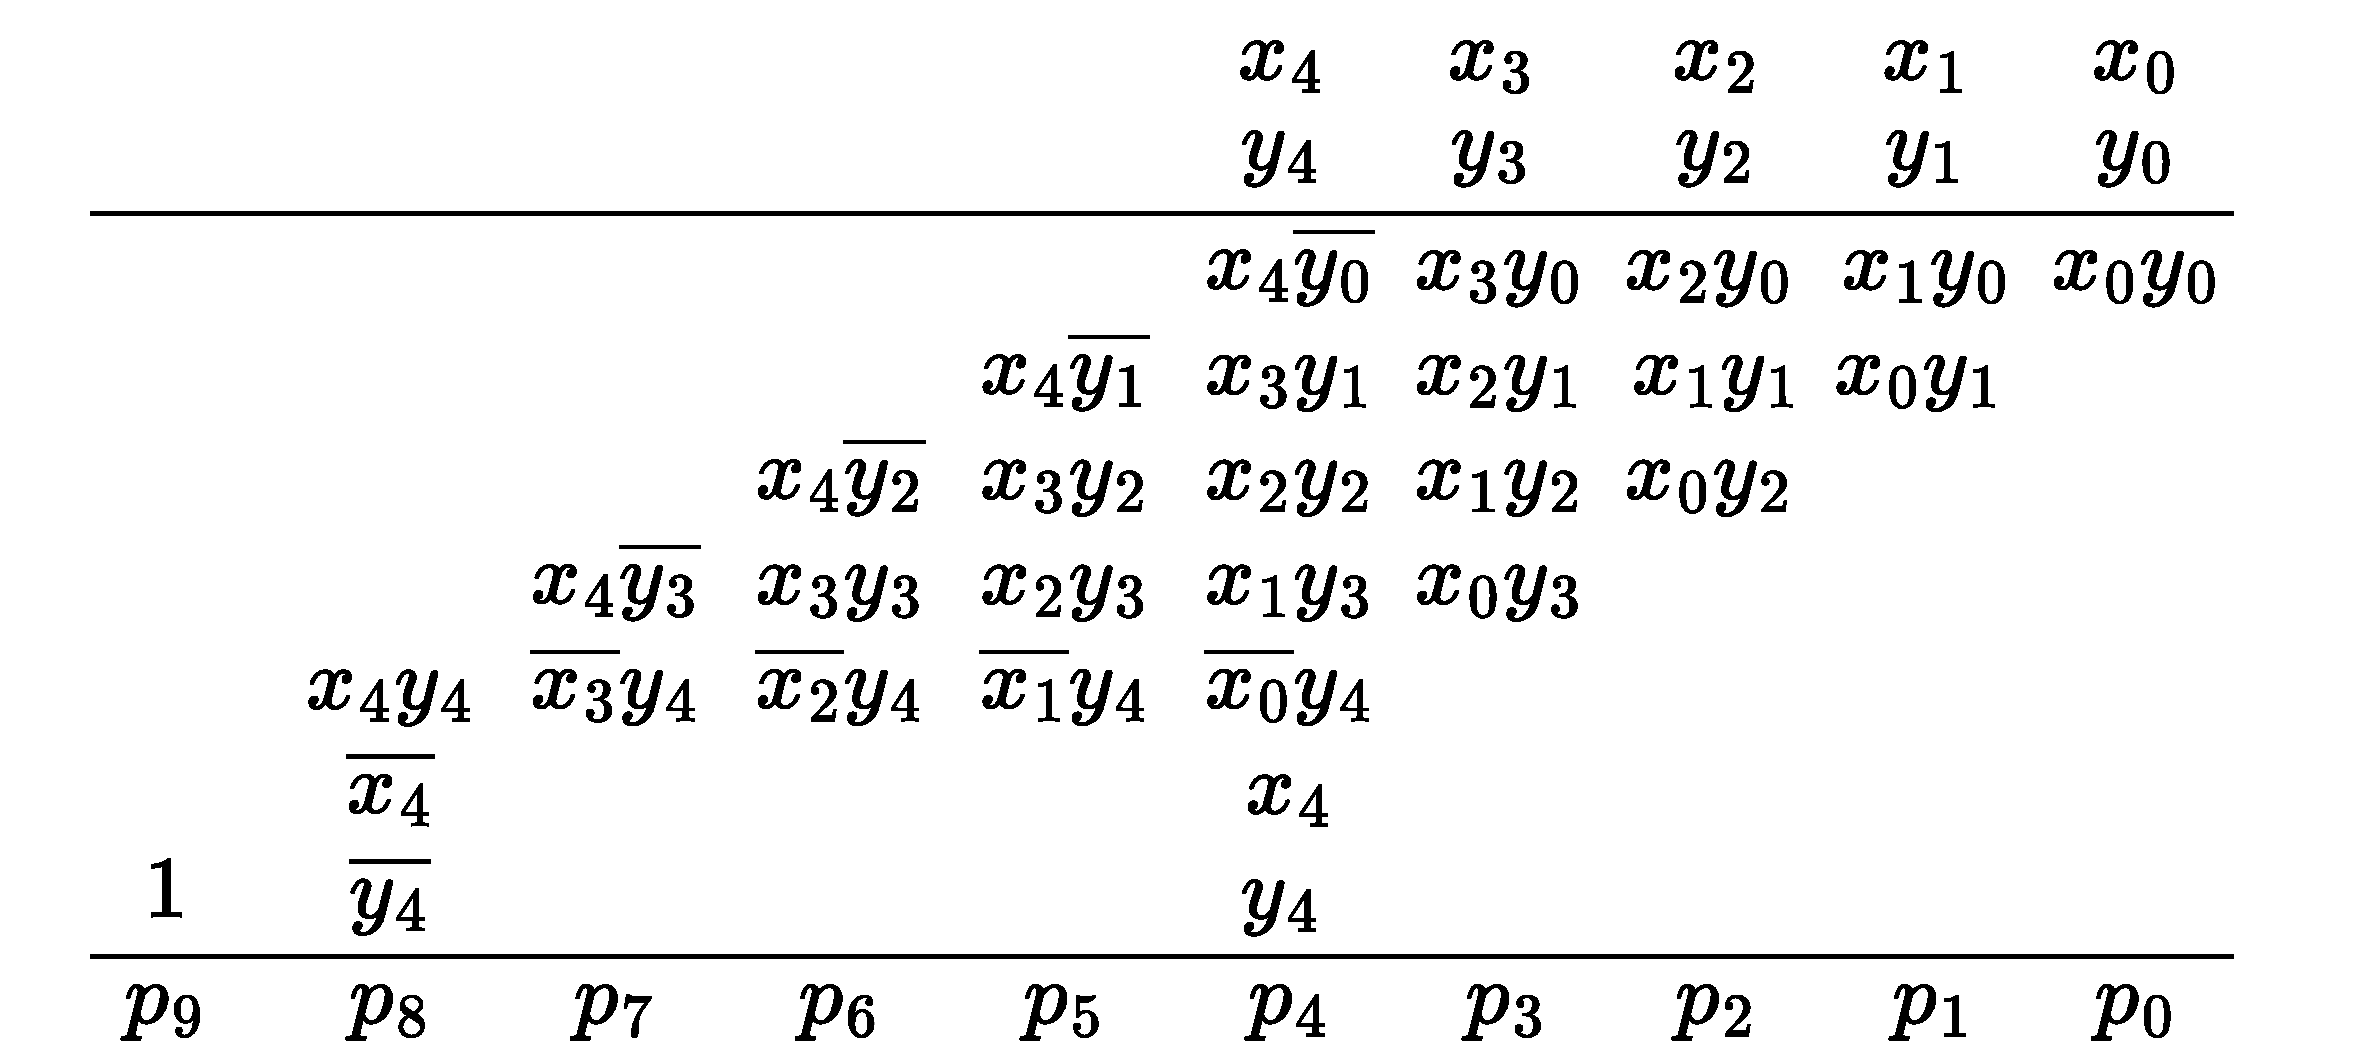
\includegraphics[width=\linewidth]{figs/EM-Fig-Baugh-Wooley.pdf}
    \end{minipage}
    }
    \subfigure[改进的Baugh-Wooley乘法器部分积阵列]{
    \label{EM:Fig:modified_Baugh-Wooley_PP}
    \begin{minipage}[t]{0.48\linewidth}
    \centering
    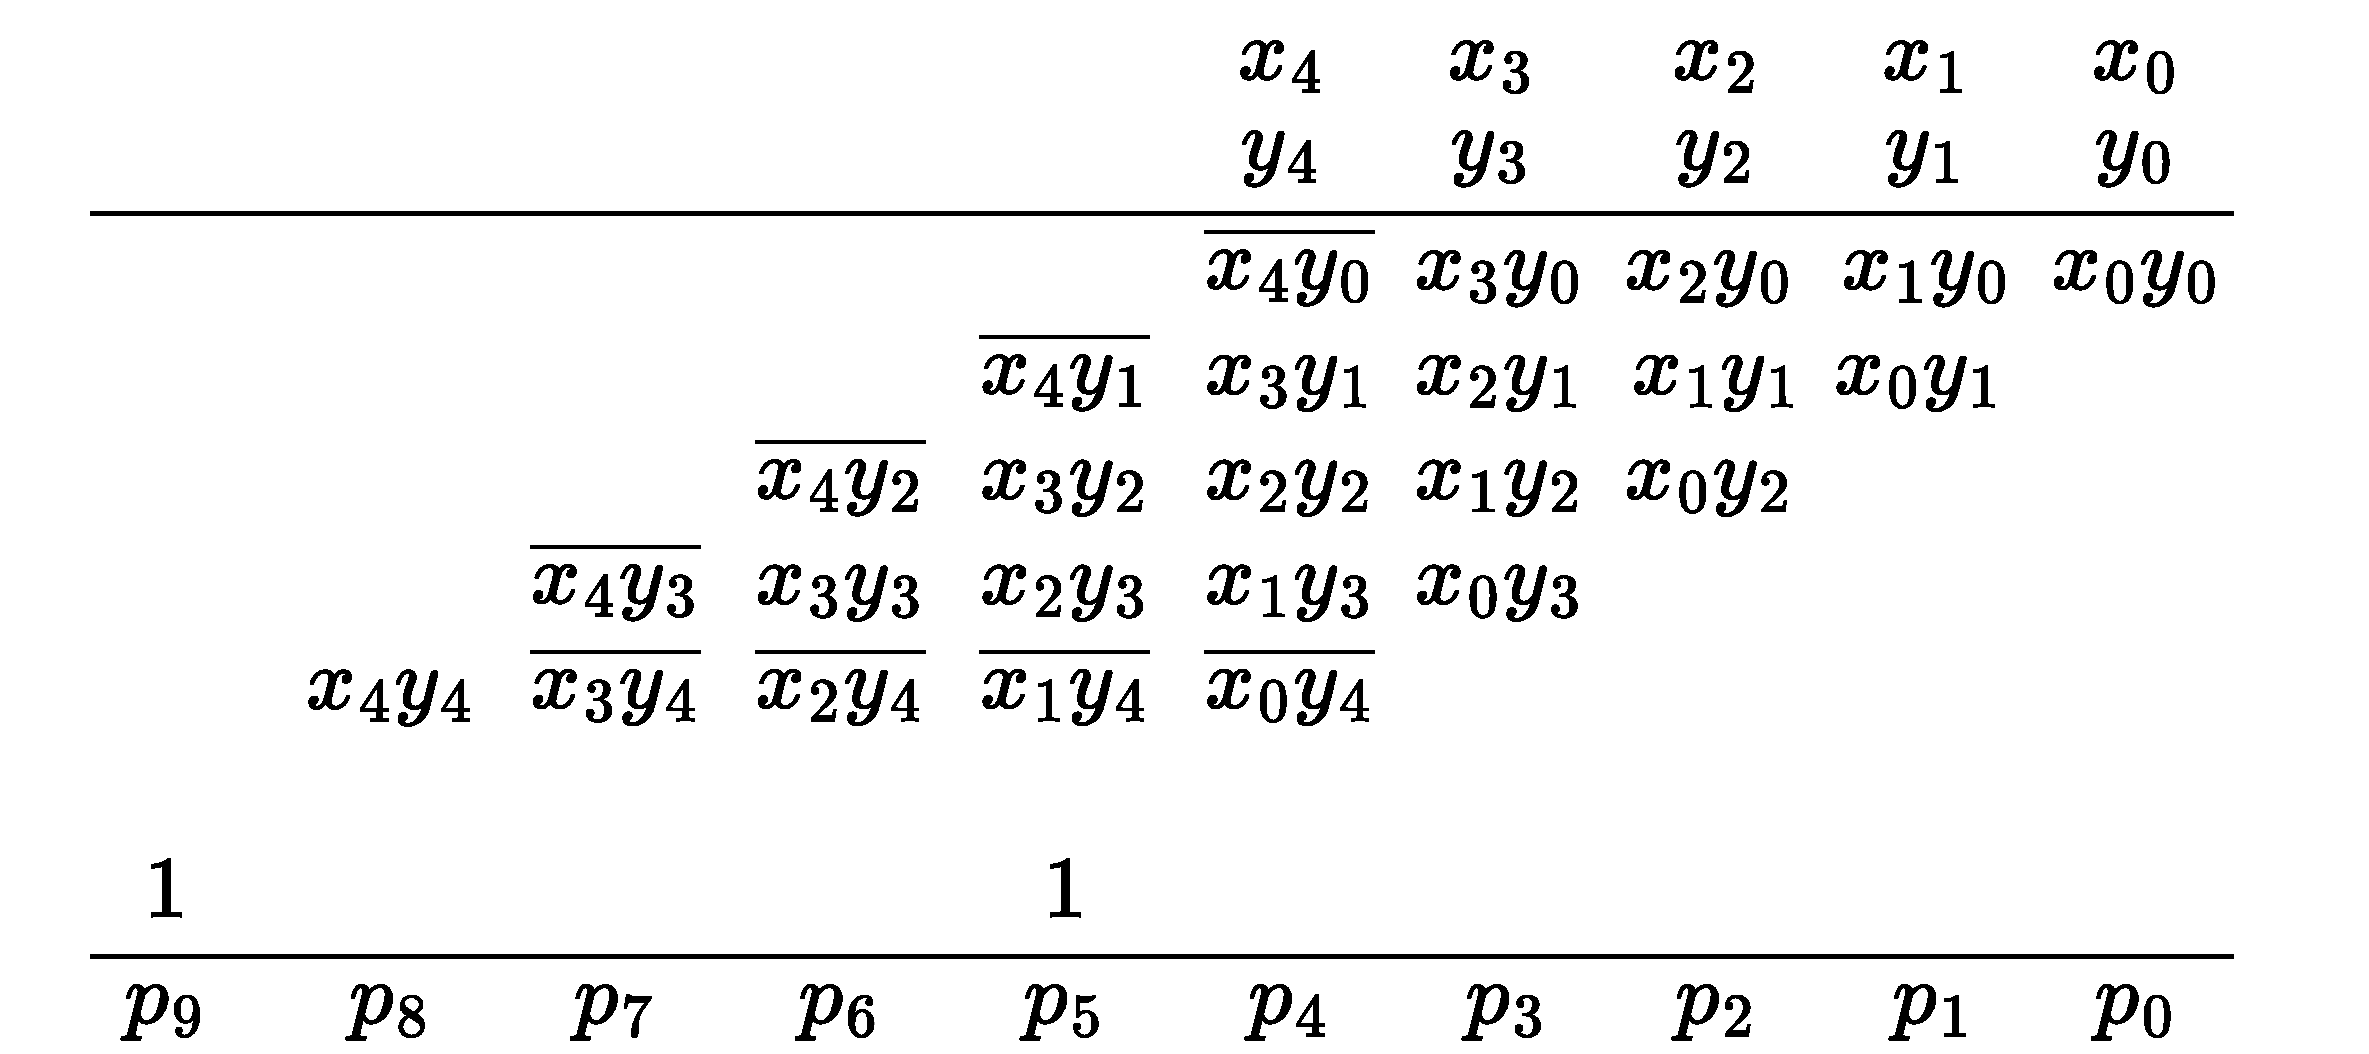
\includegraphics[width=\linewidth]{figs/EM-Fig-改进的Baugh-Wooley.pdf}
    \end{minipage}
    }
\caption{基于Baugh-Wooley算法设计的$5 \times 5$补码乘法器的部分积阵列示意图}
\label{EM:Fig:signed_comp_P_Baugh-Wooley}
\end{figure}

(3)基4的布斯编码

与Baugh-Wooley算法不同,布斯编码的意义在于能够减少乘法器中部分积的个数(行数),且基数越高效果越明显,比如基4和基8的布斯编码分别能够将部分积的个数降低一半和三分之二\cite{EM:booth_Macsorley,EM:booth_proof},大大减轻后续的累加压力。然而,高基的布斯编码电路实现复杂,目前最常用的基数是4,原理如下:

对于补码有符号乘法,假设$n$为偶数,$y_{-1} = 0$,式\eqref{EM:Eq:signed_comp_XY}中的$V(Y)$变为:
\begin{align}
    V(Y) = & \ - y_{n-1} 2^{n-1} + y_{n-2} 2^{n-2} + y_{n-3} 2^{n-3} + y_{n-4} 2^{n-4} + y_{n-5} 2^{n-5} + \cdots + \notag \\
%
    & y_5 2^5 + y_4 2^4 + y_3 2^3 + y_2 2^2 + y_1 2^1 + y_0 2^0 + \textcolor{red}{y_{-1} 2^{-1}} \notag \\
%
    = & \ ( -2 y_{n-1} + y_{n-2} + y_{n-3}) 2^{n-2} + (-2 y_{n-3} + y_{n-4} + y_{n-5}) 2^{n-4} + \cdots + \notag \\
%
    & \ (-2 y_5 + y_4 + y_3) 2^4 + (-2 y_3 + y_2 + y_1) 2^2 + (-2 y_1 + y_0 + \textcolor{red}{y_{-1}} ) 2^0
\label{EM:Eq:Radix-4-booth_VY}
\end{align}
式\eqref{EM:Eq:signed_comp_P}变为:
\begin{align}
    V(P) = & \ V(X)V(Y) \notag \\
    = & \ V(X) ( -2 y_{n-1} + y_{n-2} + y_{n-3}) 2^{n-2} + \notag \\
%
    & \ V(X) (-2 y_{n-3} + y_{n-4} + y_{n-5}) 2^{n-4} + \cdots + \notag \\
%
    & \ V(X) (-2 y_5 + y_4 + y_3) 2^4 + \notag \\
    & \ V(X) (-2 y_3 + y_2 + y_1) 2^2 + \notag \\
    & \ V(X) (-2 y_1 + y_0 + \textcolor{red}{y_{-1}} ) 2^0
    \label{EM:Eq:Radix-4-booth}
\end{align}
即是基4的布斯编码算法公式,其中$X$是被乘数,$Y$是乘数,对应的编码规则及部分积操作如表\ref{EM:Tab:Radix-4-booth}所示。该算法在进行前需要在乘数的最右侧隐含地补一个0,之后从最低有效位开始每次扫描3位乘数生成部分积,共$\dfrac{n}{2}$个,然后对部分积进行符号位扩展、累加并最终相加。由表\ref{EM:Tab:Radix-4-booth}可以看出,基4的布斯算法只涉及加法、减法和移位操作,硬件实现友好。
需要注意的是,式\eqref{EM:Eq:Radix-4-booth}仅适用于$n$是偶数的情况,若$n$是奇数,需先对乘数进行一位符号位扩展,将位宽变为偶数,之后再进行编码,此时部分积总数变为$\dfrac{n+1}{2}$个。布斯编码得到的部分积仍然需要符号位扩展,扩展后的累加电路复杂,可考虑采用改进的符号位扩展方法对其进行优化。

\begin{table}
\centering
\caption{基4布斯编码表}
\begin{tabular}{|c|c|c|c|c|} \hline
$y_{i+1}$ & $y_i$ & $y_{i-1}$ & $-2 y_{i+1} + y_i + y_{i-1}$ & \text{部分积操作} \\ \hline
0 & 0 & 0 & 0 & +0 \\ \hline
0 & 0 & 1 & 1 & $+[X]_{\text{补}}$ \\ \hline
0 & 1 & 0 & 1 & $+[X]_{\text{补}}$ \\ \hline
0 & 1 & 1 & 2 & $+2[X]_{\text{补}}$ \\ \hline
1 & 0 & 0 & -2 & $-2[X]_{\text{补}}$ \\ \hline
1 & 0 & 1 & -1 & $-[X]_{\text{补}}$ \\ \hline
1 & 1 & 0 & -1 & $-[X]_{\text{补}}$ \\ \hline
1 & 1 & 1 & 0 & +0 \\ \hline
\end{tabular}
\label{EM:Tab:Radix-4-booth}
\end{table}

除了补码有符号数乘法,布斯算法也可以用于无符号数相乘%
\IfStrEq{\Version}{Open}{%
    \footnote{\url{https://picture.iczhiku.com/resource/eetop/whKDFaTwqTZOkCxn.pdf}},
}{,}
为了支持布斯编码中需要的减法操作,无符号乘法的部分积也应采用补码格式。若基数取4,编码形式仍然是$-2 y_{i+1} + y_i + y_{i-1}$,但与补码乘法的区别在于:(a)$n$是偶数时需要添加的不仅是$y_{-1} = 0$,还有$y_{n+1} = y_n = 0$,此时$\{y_{n+1}, y_n, y_{n-1} \}$编码得到的部分积一定是0或正数,部分积总数为$\dfrac{n}{2} + 1$个;(b)$n$是奇数时需要添加$y_n = y_{-1} = 0$,部分积总数为$\dfrac{n+1}{2}$个;(c)改进的符号位扩展方法实现细节略有不同。

下面具体讲解基4布斯算法在无符号数乘法和补码有符号数乘法中,如何对部分积符号位扩展方法进行改进\cite{EM:booth_sign_extension}:


\begin{figure}[!htb]
    \centering
    \subfigure[部分积均为正数,省略了高位的0扩展]{
    \label{EM:Fig:booth_16x16_unsign_PP_positive}
    \begin{minipage}[t]{0.48\linewidth}
    \centering
    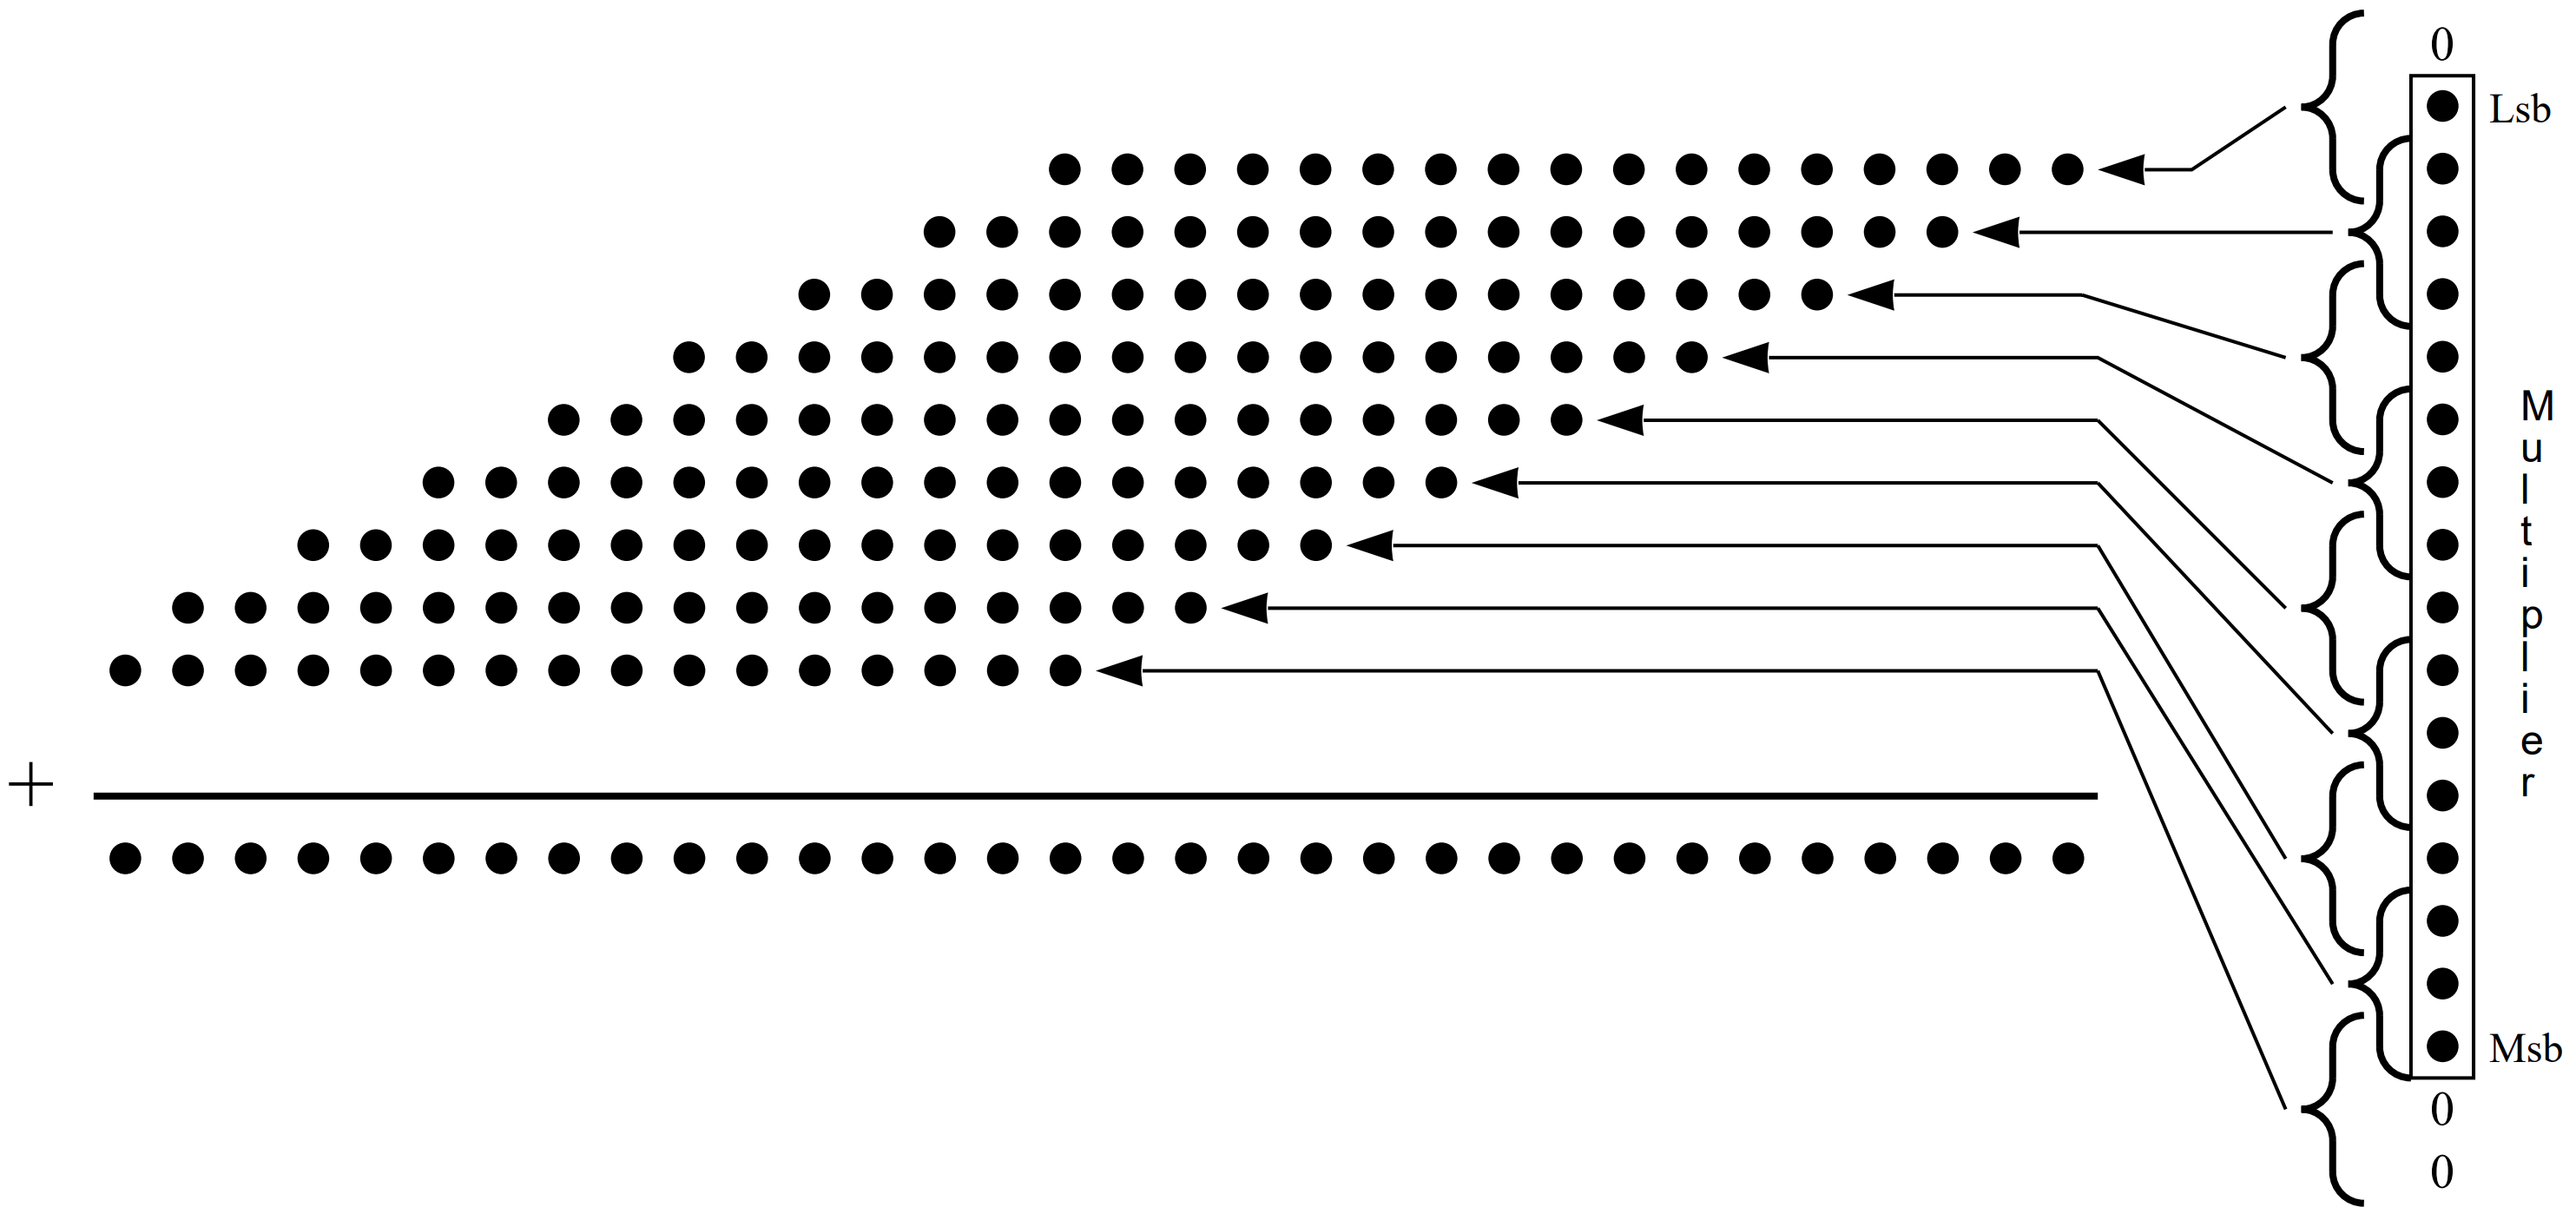
\includegraphics[width=\linewidth]{figs/EM-Fig-booth_unsign_positive.png}
    \end{minipage}
    }
    \subfigure[部分积均为负数,高位进行1扩展]{
    \label{EM:Fig:booth_16x16_unsign_PP_negtive}
    \begin{minipage}[t]{0.48\linewidth}
    \centering
    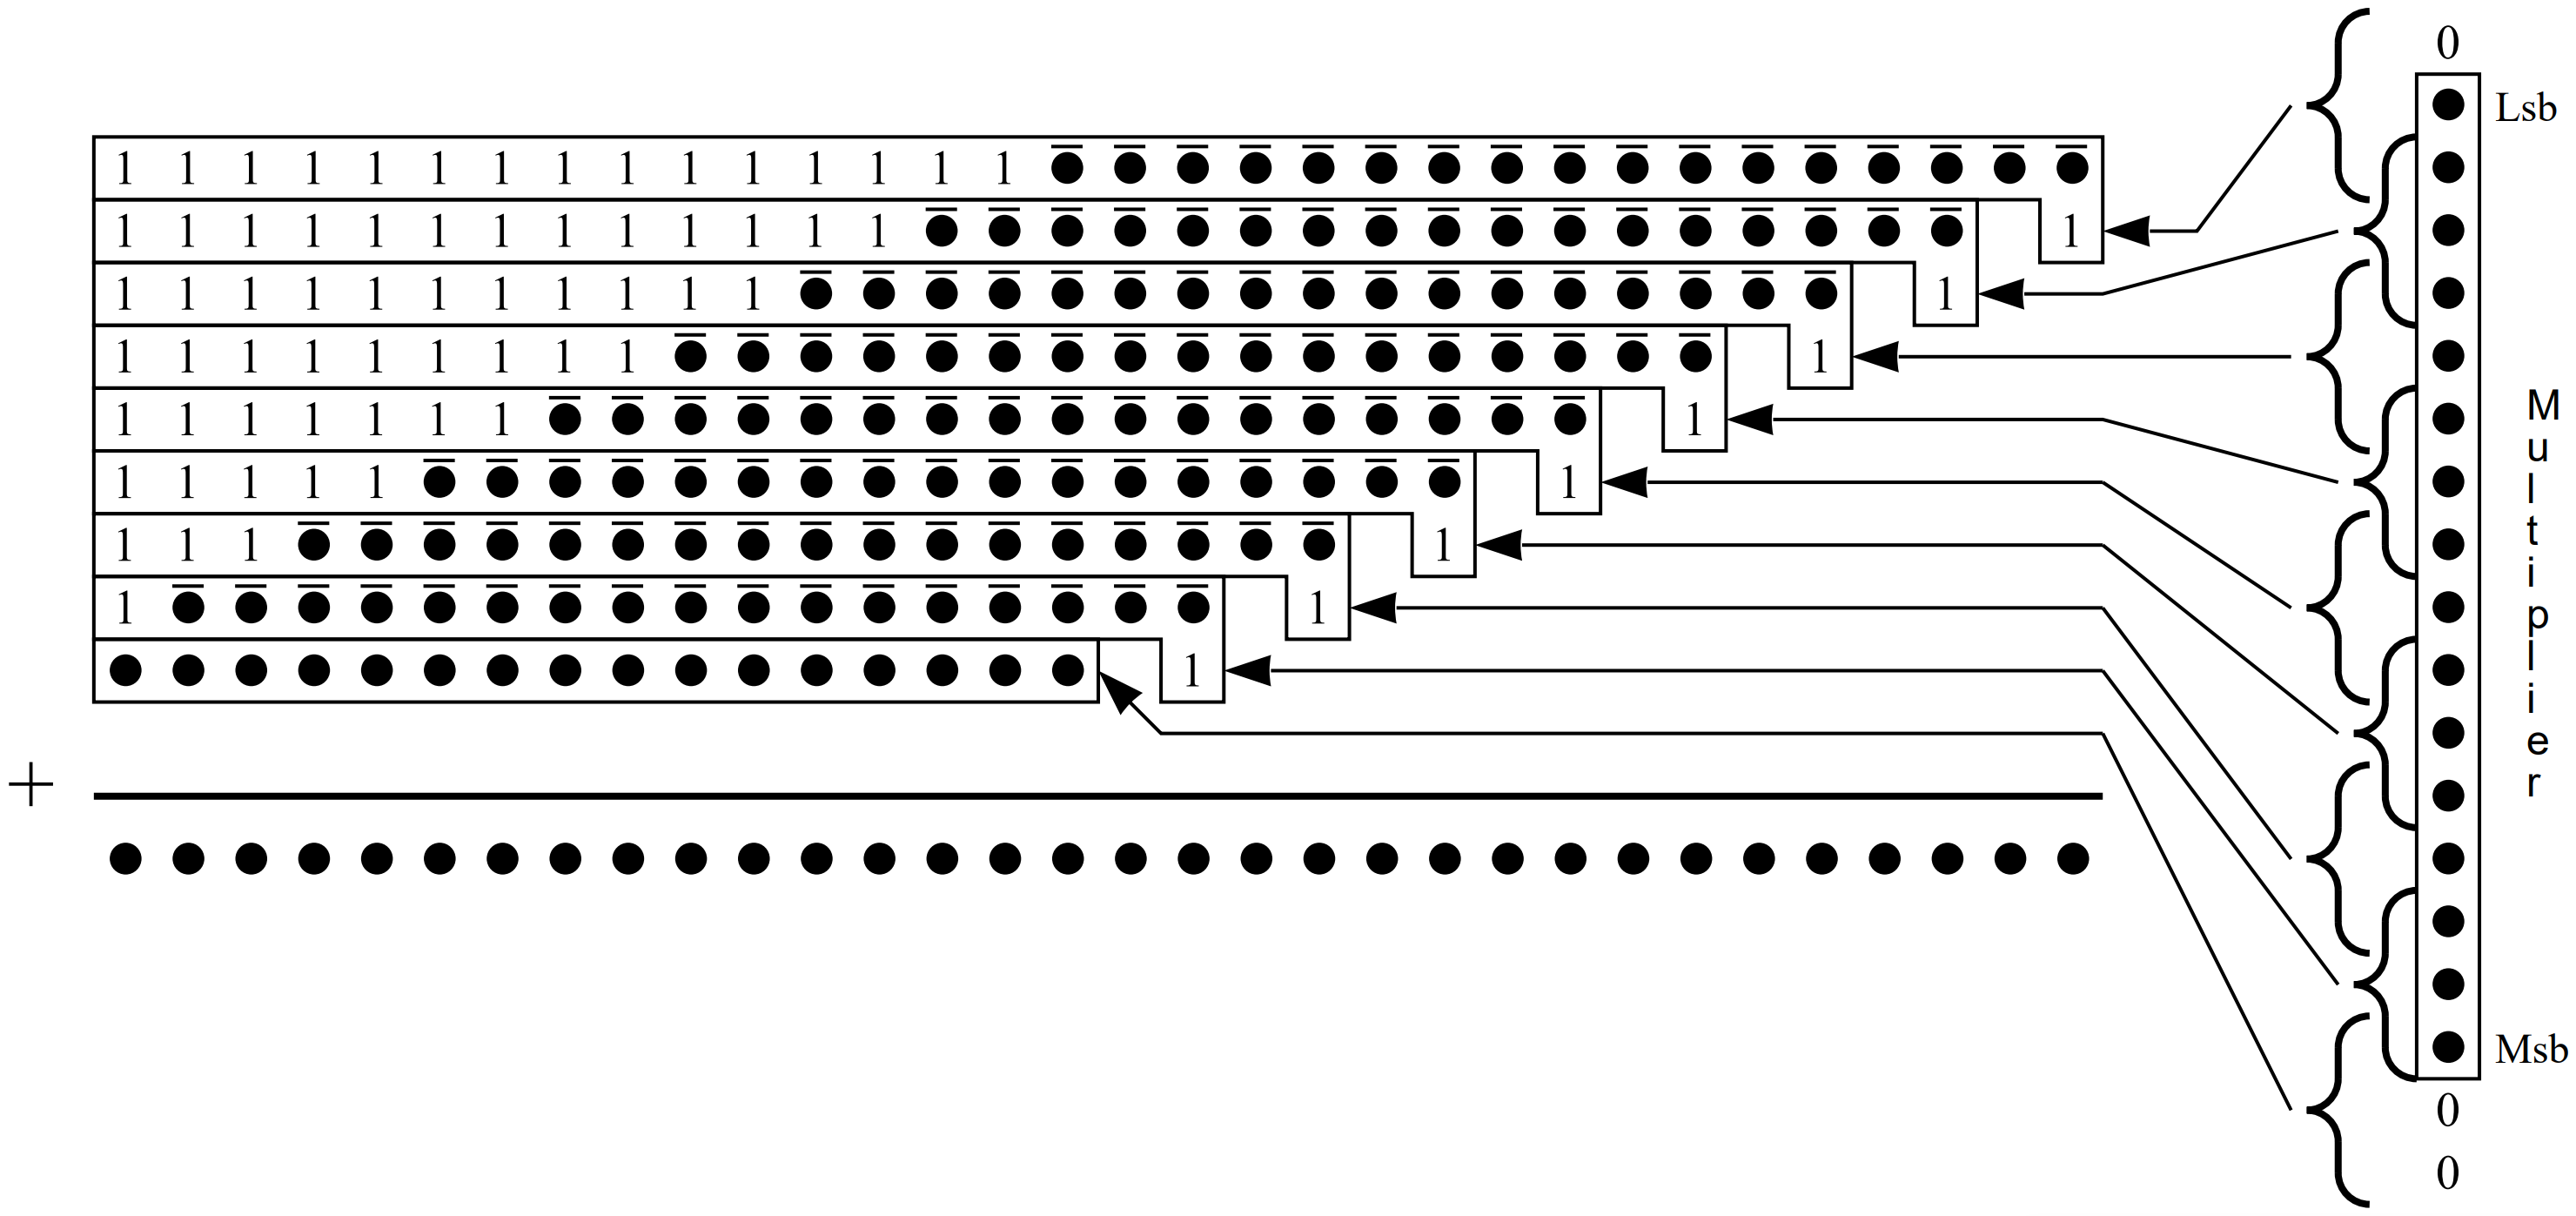
\includegraphics[width=\linewidth]{figs/EM-Fig-booth_unsign_negtive.png}
    \end{minipage}
    }
    \subfigure[部分积均为负数,高位进行1扩展后累加]{
    \label{EM:Fig:booth_16x16_unsign_PP_negtive_summed}
    \begin{minipage}[t]{0.48\linewidth}
    \centering
    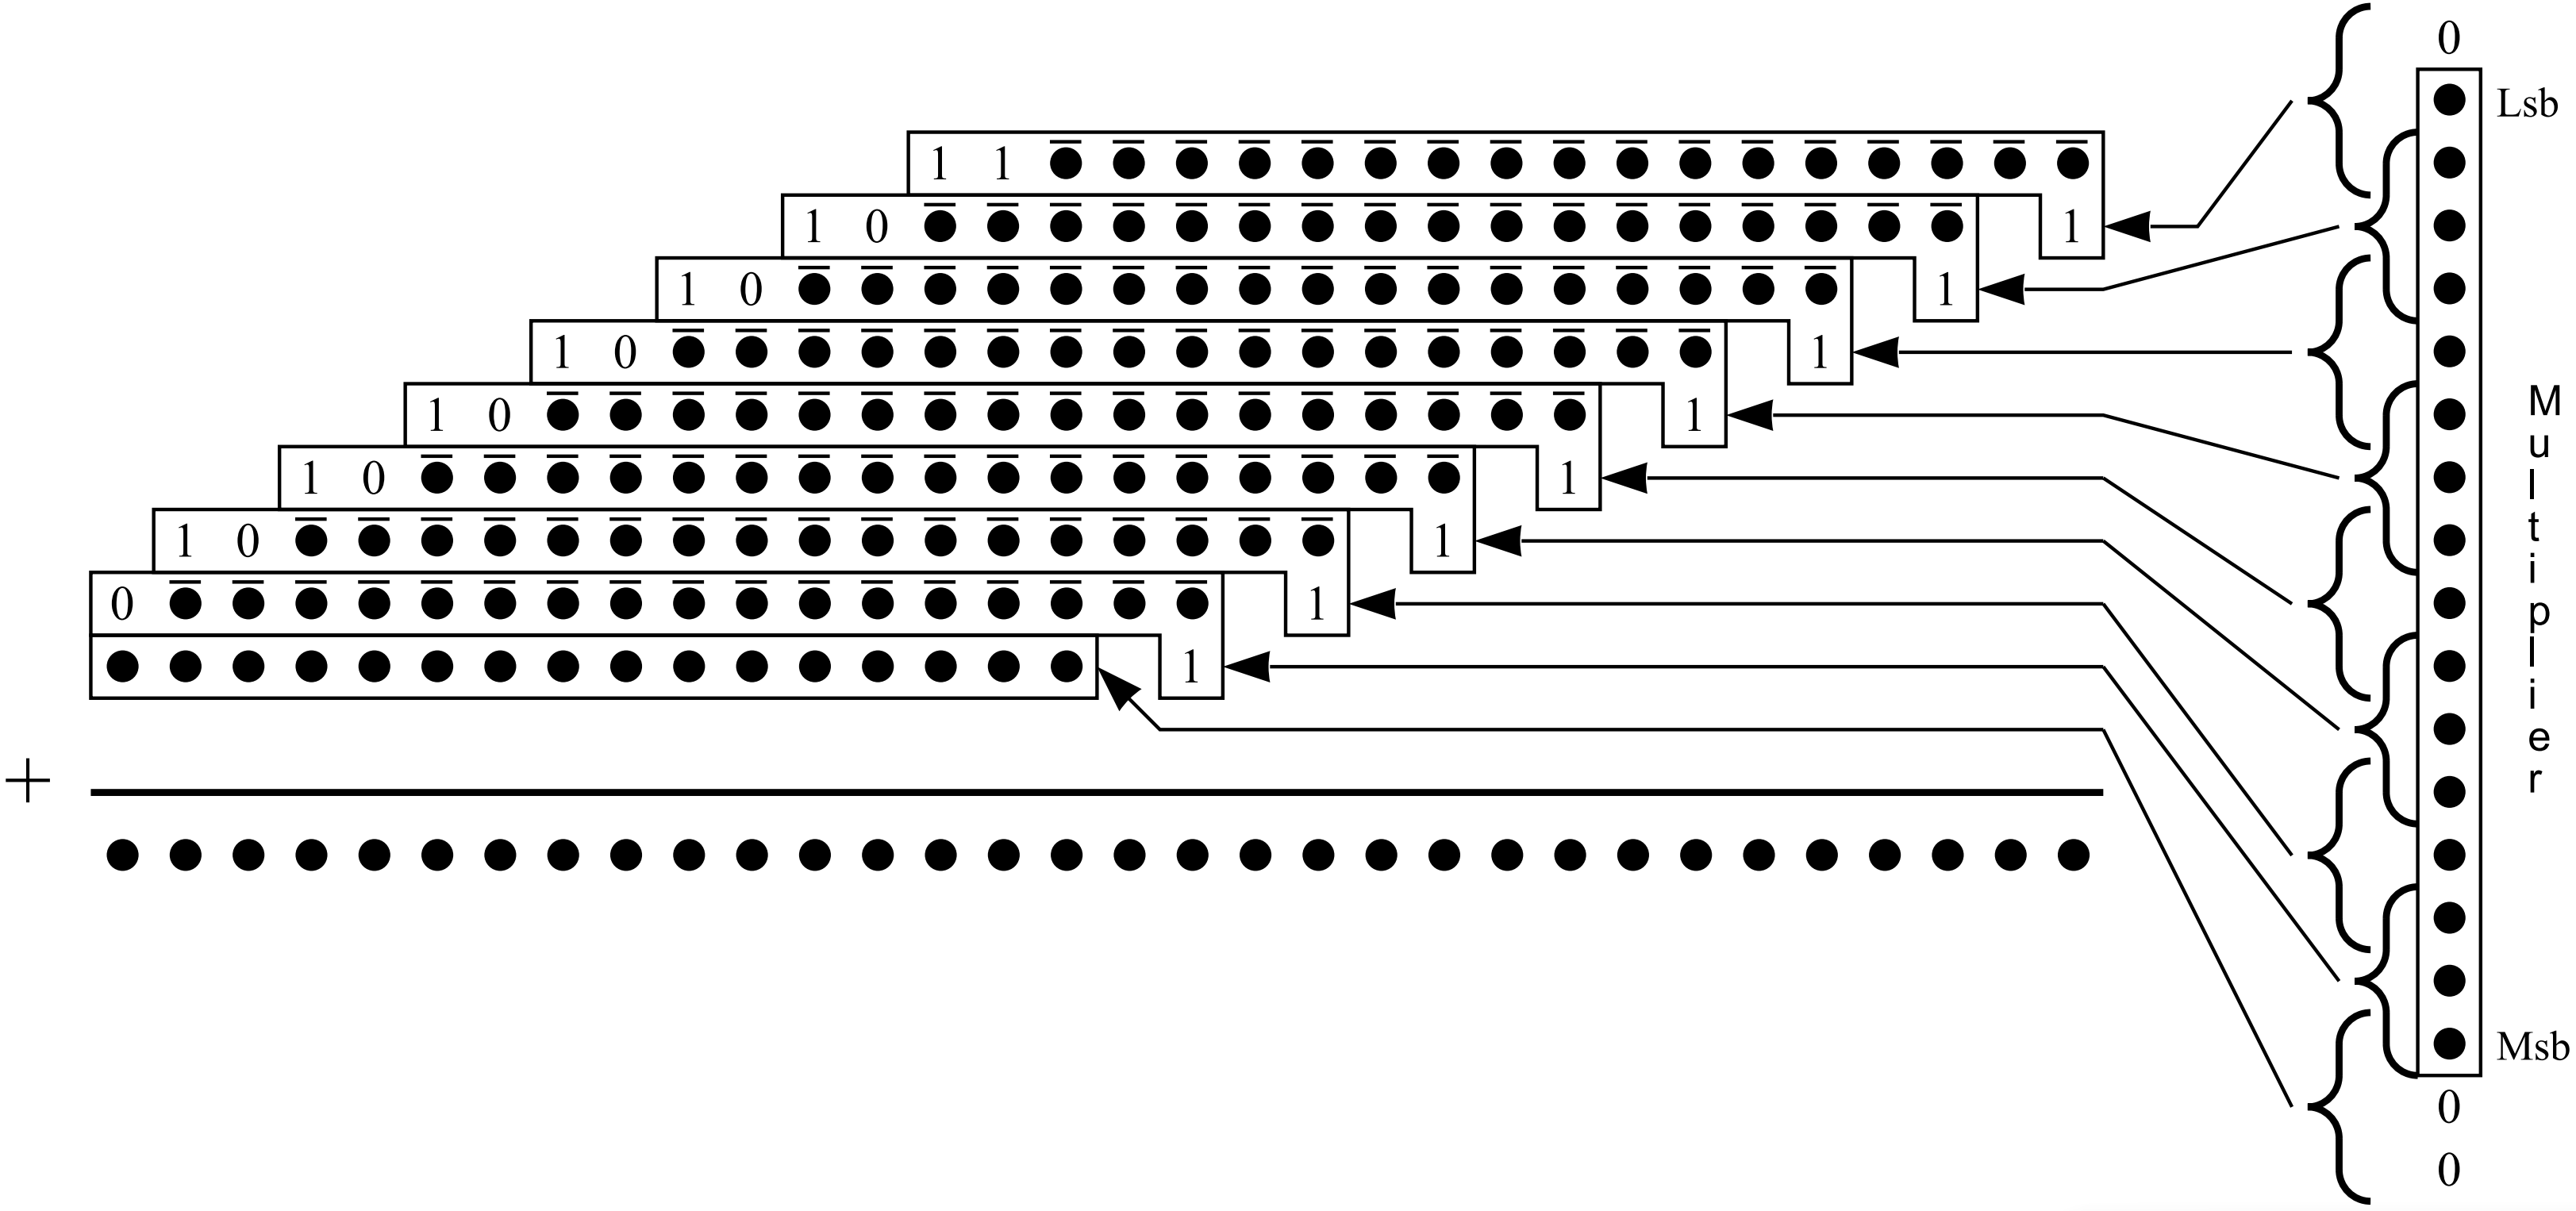
\includegraphics[width=\linewidth]{figs/EM-Fig-booth_unsign_negtive_summed.png}
    \end{minipage}
    }
    \subfigure[部分积正负均可的统一符号位扩展方法,$S$表示布斯码值的符号,$S=0$为正,$S=1$为负]{
    \label{EM:Fig:booth_16x16_unsign_PP_complete}
    \begin{minipage}[t]{0.48\linewidth}
    \centering
    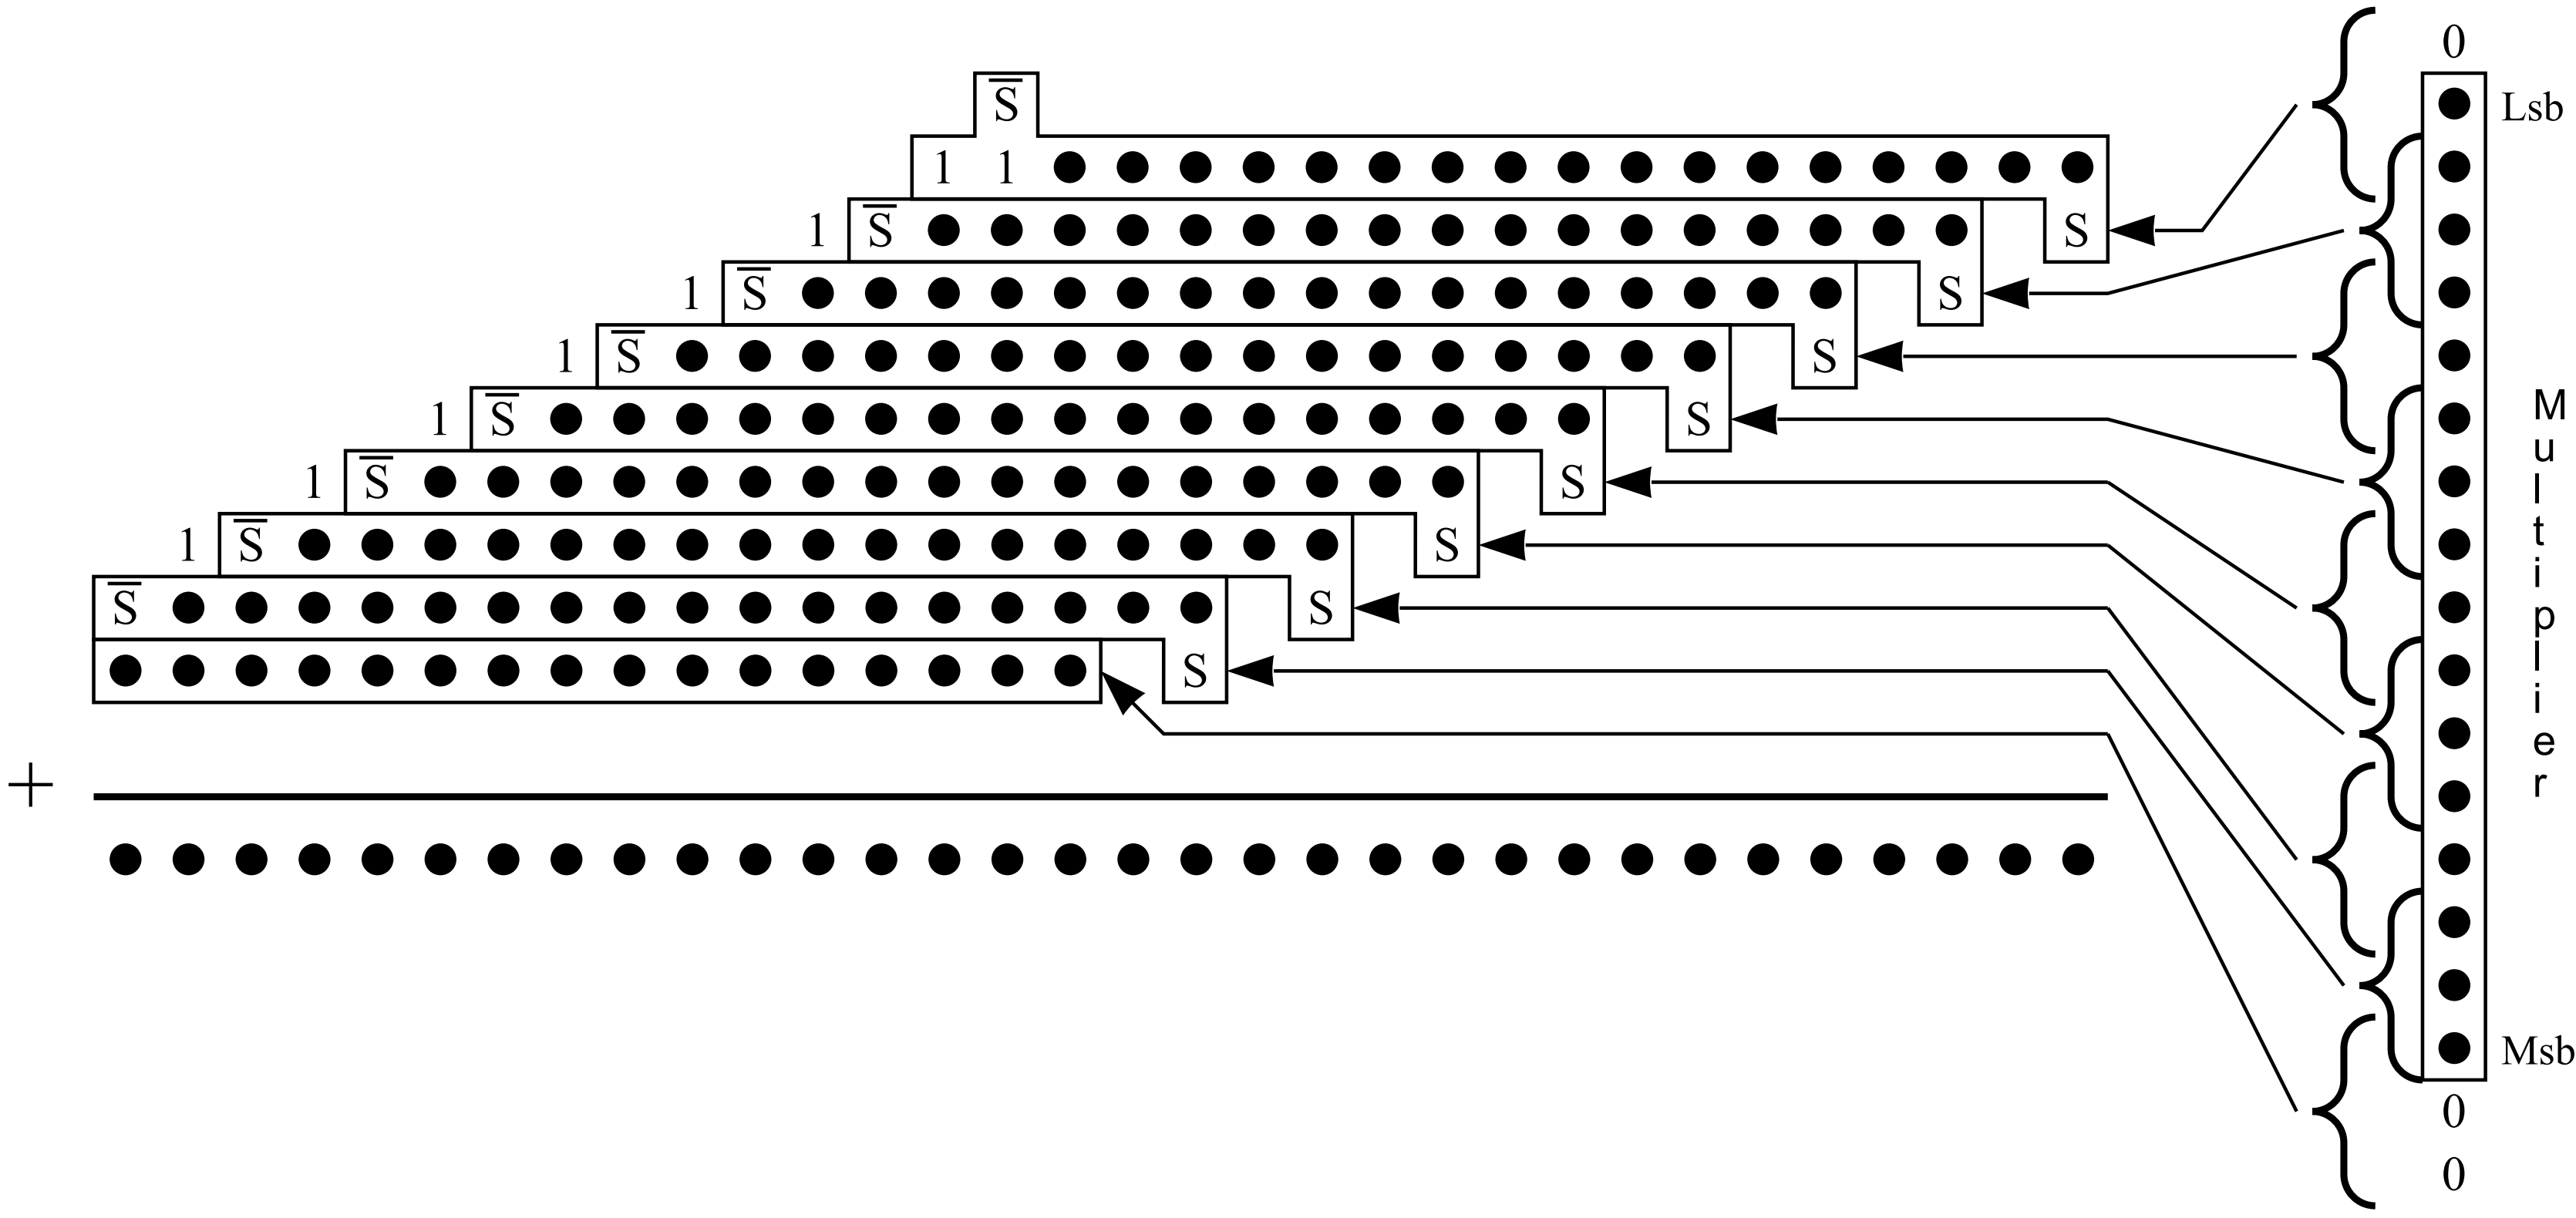
\includegraphics[width=\linewidth]{figs/EM-Fig-booth_unsign_complete.png}
    \end{minipage}
    }
    \subfigure[利用等价变换降低阵列层数后的部分积符号位扩展方法,$S$表示布斯码值的符号,$S=0$为正,$S=1$为负]{
    \label{EM:Fig:booth_16x16_unsign_PP_complete_reduce_height}
    \begin{minipage}[t]{0.48\linewidth}
    \centering
    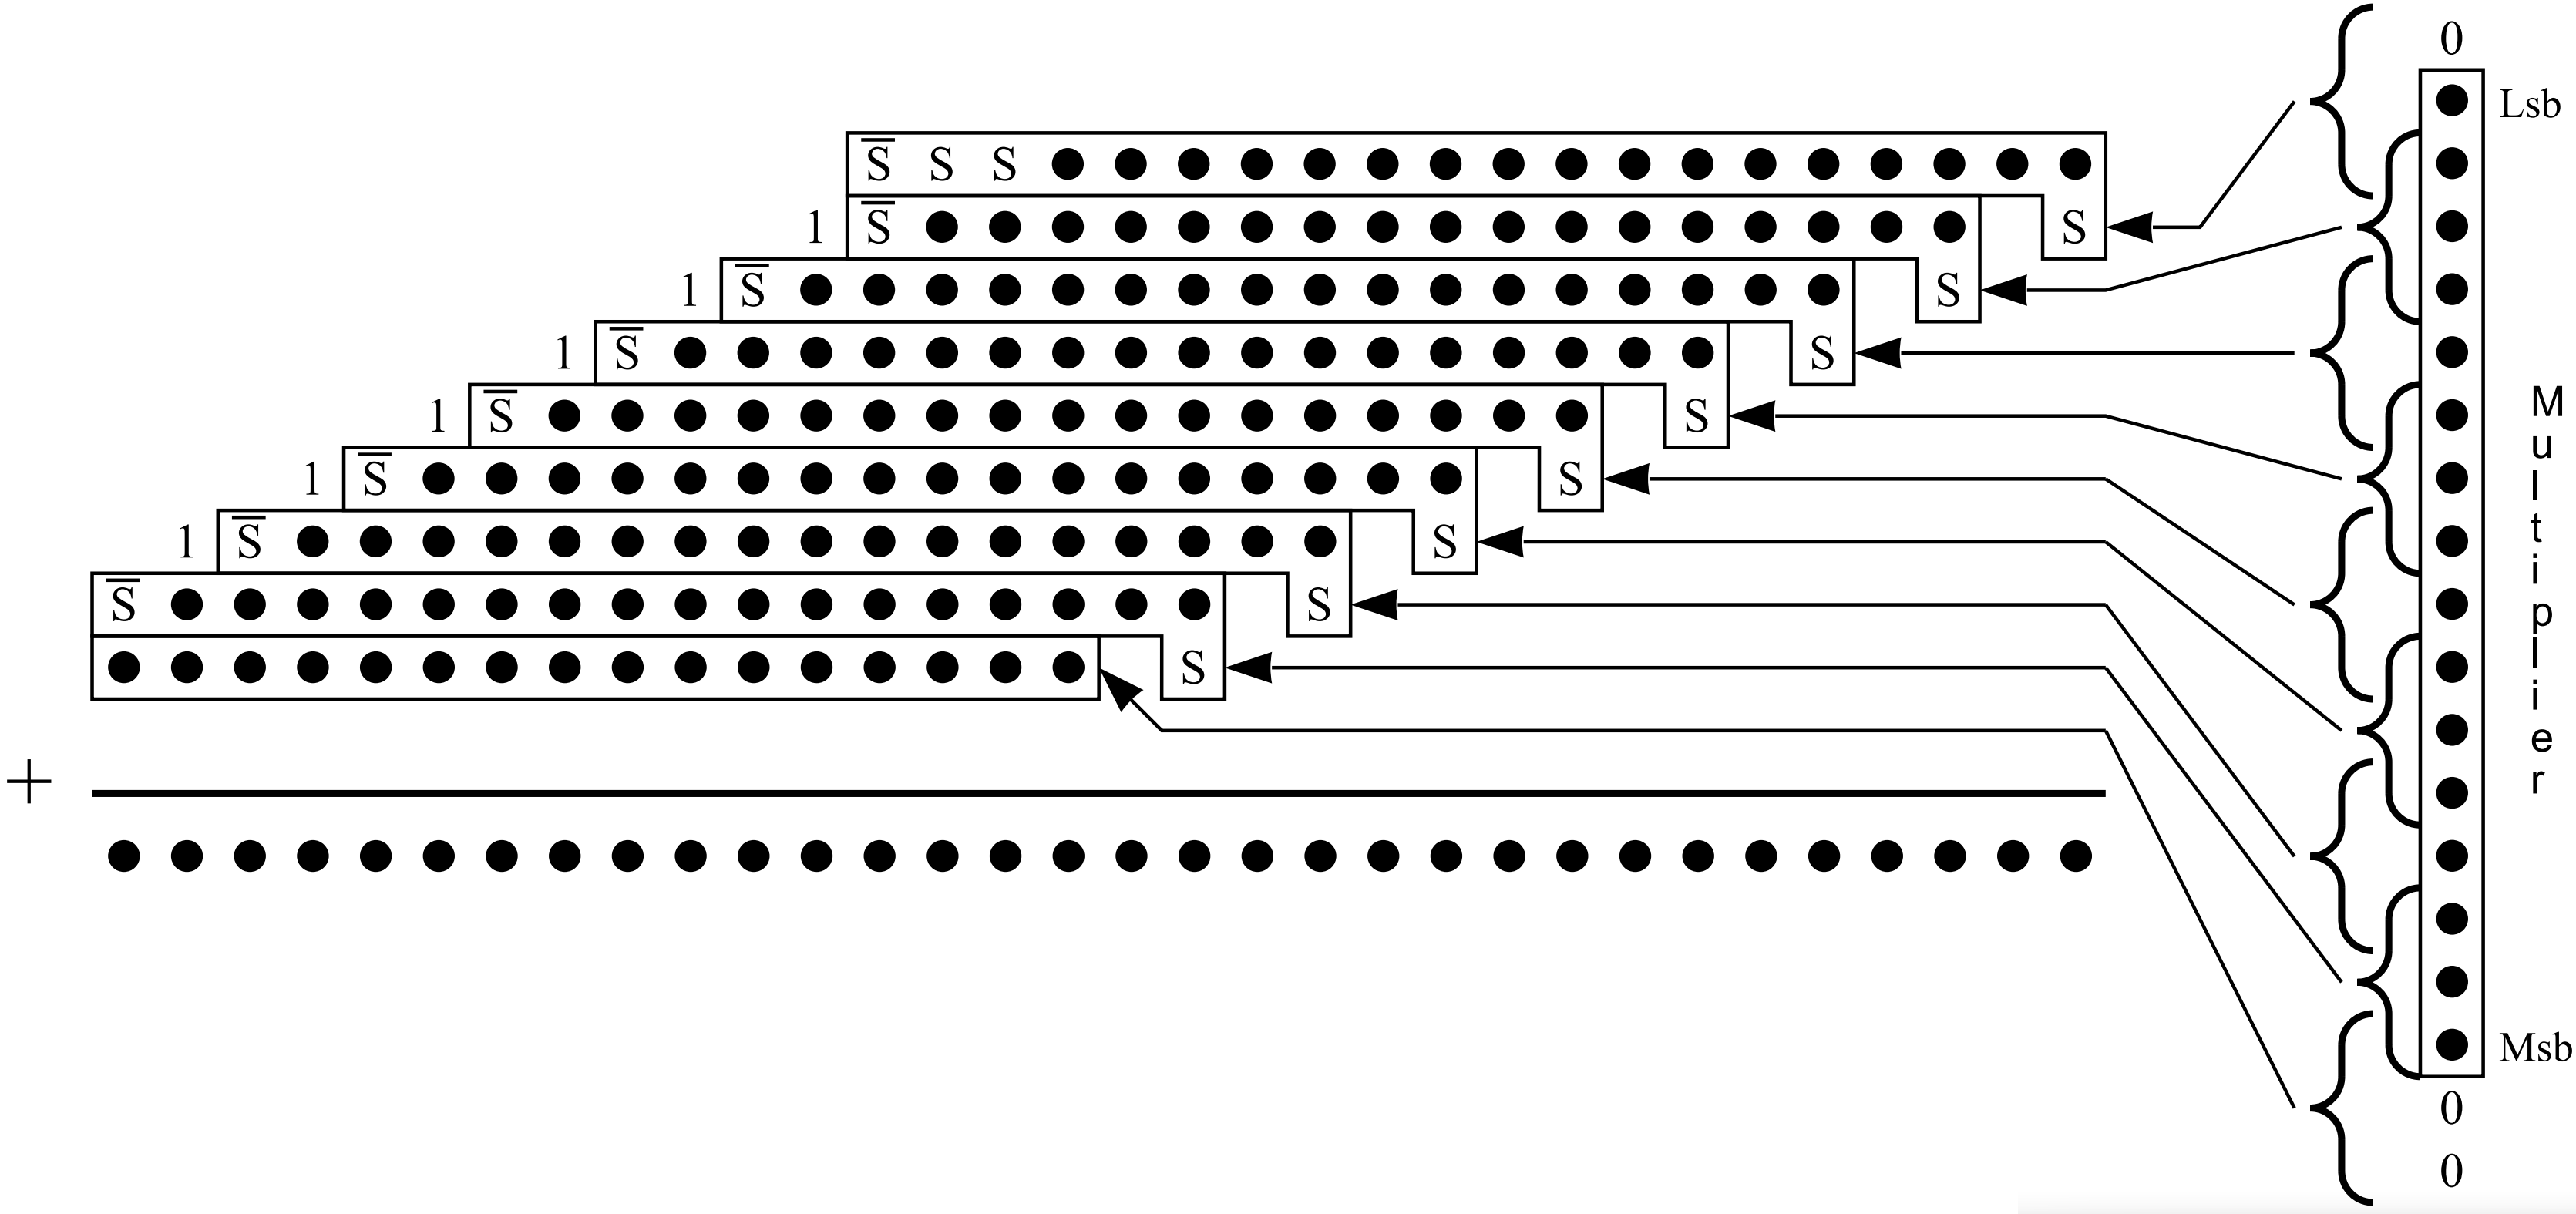
\includegraphics[width=\linewidth]{figs/EM-Fig-booth_unsign_complete_reduce_height.png}
    \end{minipage}
    }
\caption{$16\times16$无符号乘法的基4布斯算法部分积符号位扩展的改进办法}
\label{EM:Fig:booth_16x16_unsign_PP}
\end{figure}

对于$16\times16$无符号数乘法,假设每个部分积是非负数,高位应进行0扩展,0可省略,省略后的部分积阵列如图\ref{EM:Fig:booth_16x16_unsign_PP_positive}所示,部分积总数为$8+1 = 9$个。除了最下面的那个部分积之外,每个部分积的位宽均为17比特。不考虑最下面的那个部分积(该部分积永远是非负数),图\ref{EM:Fig:booth_16x16_unsign_PP_negtive}展示了所有部分积均为负数时的符号位扩展情况,即高位进行1扩展,对扩展产生的大量的1进行累加后的部分积阵列如图\ref{EM:Fig:booth_16x16_unsign_PP_negtive_summed}所示。
若图\ref{EM:Fig:booth_16x16_unsign_PP_negtive_summed}中存在部分积为正值,则需要对部分积的符号位进行修正,将高位的1扩展变回为0扩展,方法如图\ref{EM:Fig:booth_16x16_unsign_PP_complete}所示,引入$S$代表布斯码值的符号,$S=0$表示布斯码值为正,$S=1$表示布斯码值为负,达到对部分积进行统一符号位扩展的效果。最后,通过等价变换将\ref{EM:Fig:booth_16x16_unsign_PP_complete}中最上面的$\overline{S}$合并在部分积中,降低部分积阵列的层数,最终结果如图\ref{EM:Fig:booth_16x16_unsign_PP_complete_reduce_height}所示,即为16$\times$16无符号基4布斯算法的符号位扩展改进方法。

对于补码有符号布斯算法,当乘数的位宽为偶数时,部分积的个数会比同位宽的无符号布斯算法少一个。在符号位扩展方面的区别是,假设部分积均为负数而实际可能为正数、将大量的1累加后、需要对部分积的符号位进行修正时,不能单一的通过引入布斯码值的符号进行修正,而是要引入布斯码值的符号$S$和被乘数符号位的同或(Exclusive-NOR)进行修正。图\ref{EM:Fig:booth_16x16_signed_PP}展示了$16\times16$补码乘法的基4布斯算法部分积符号位扩展的改进方法示意图。
\begin{figure}[!htb]
    \centering
    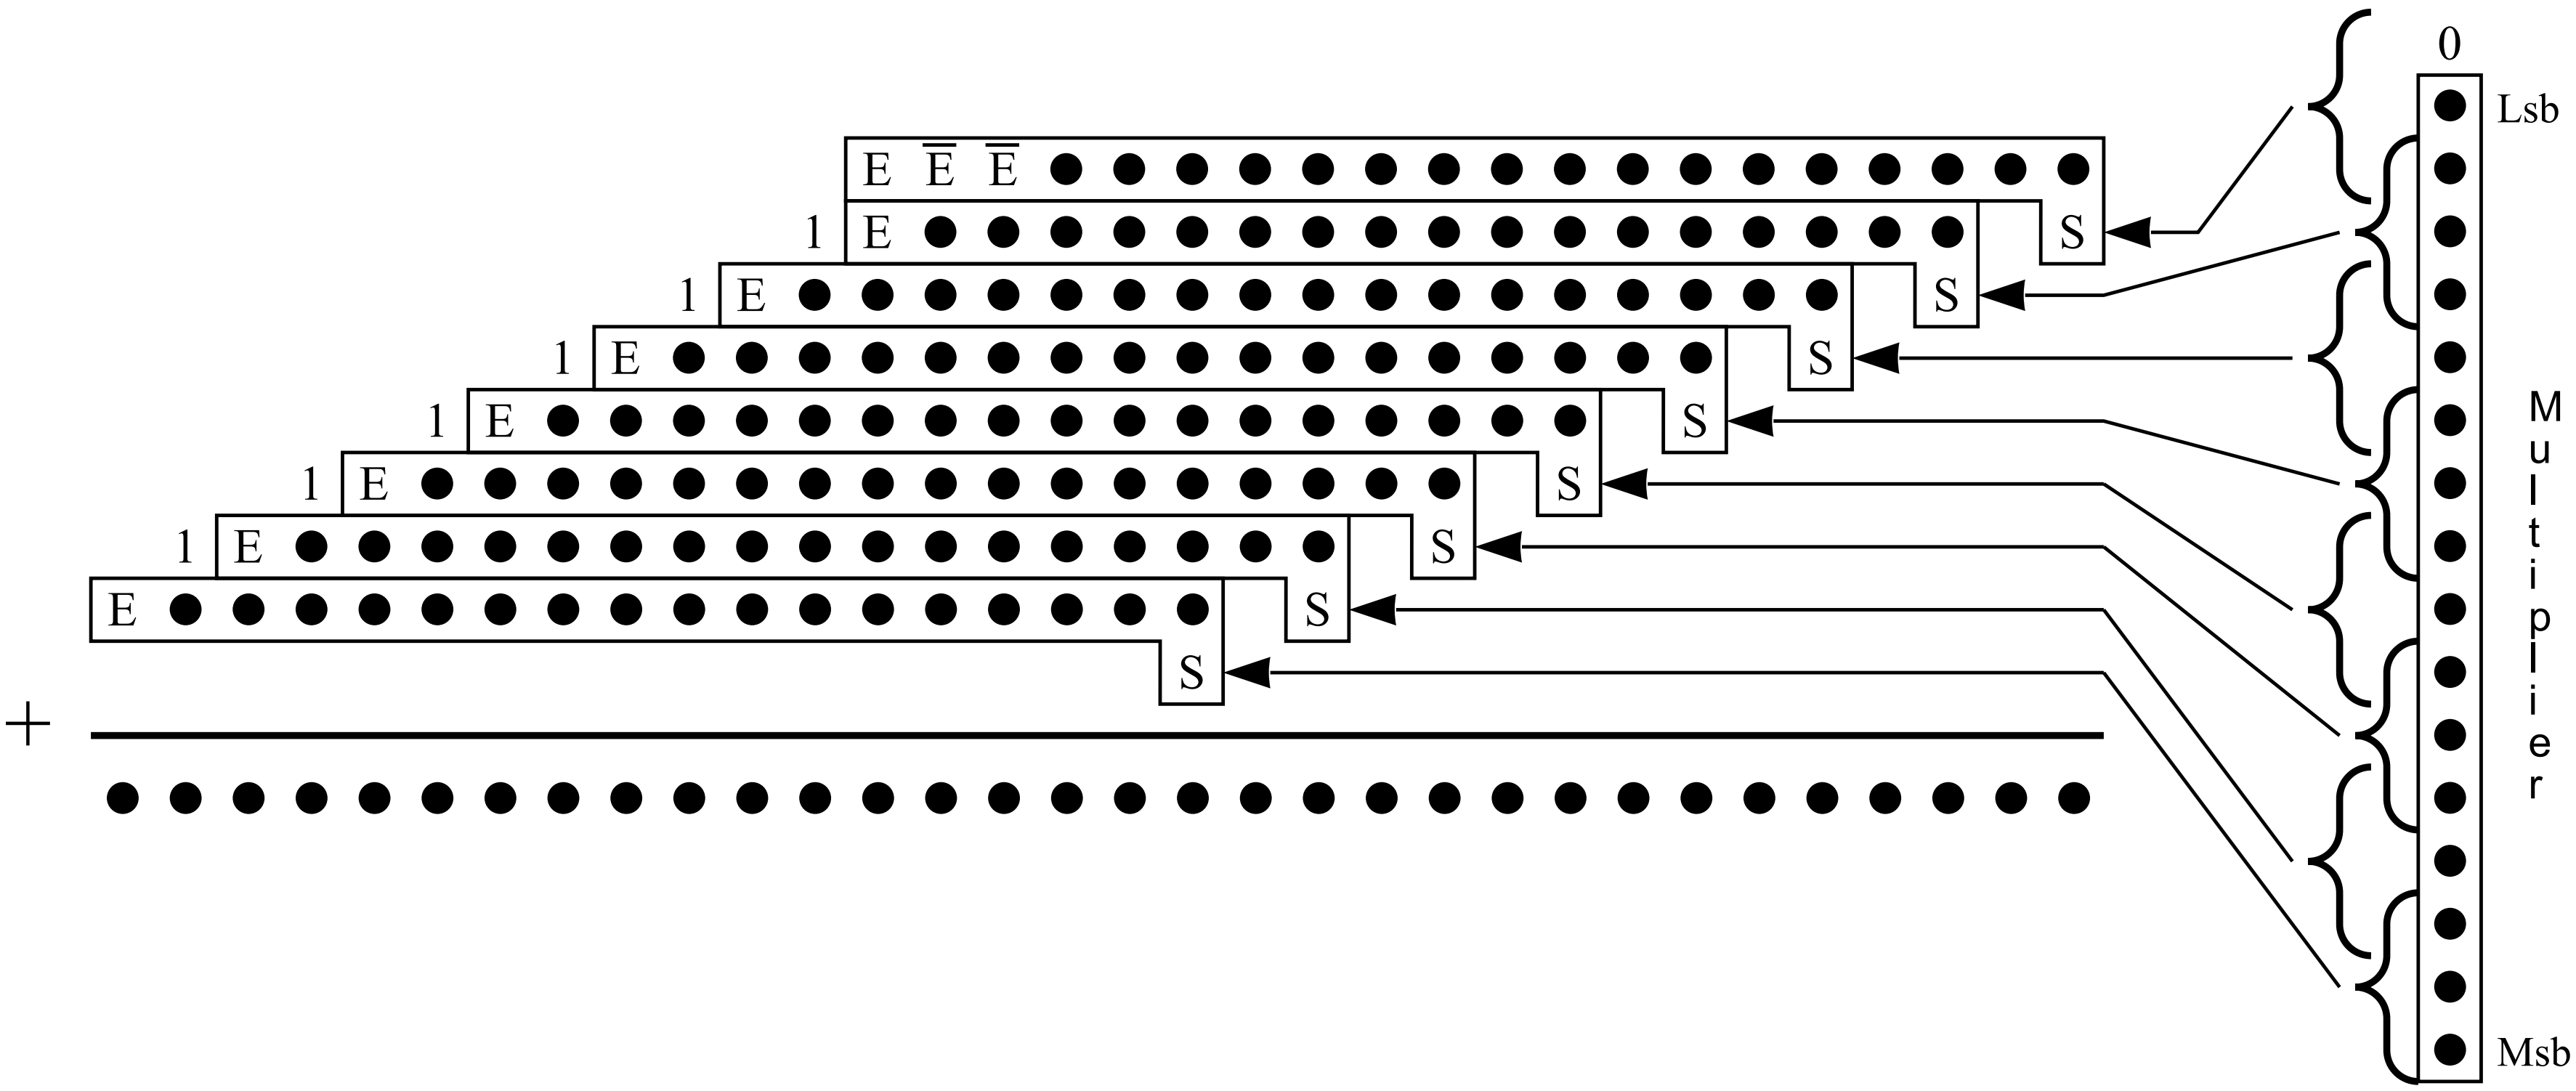
\includegraphics[width=\textwidth]{figs/EM-Fig-booth_signed.png}
    \caption{$16 \times 16$补码乘法的基4布斯算法部分积符号位扩展的改进方法,$E$表示布斯码值的符号$S$和被乘数符号位同或之后的结果}
    \label{EM:Fig:booth_16x16_signed_PP}
\end{figure}

\subsection{部分积的累加}

部分积产生后需要进行累加,这种累加本质上是一种多操作数的加法。一个直接的累加方式是用许多全加器(Full Adder, FA)组成阵列进行运算,被称为阵列累加,更为先进的方法是以进位保留或树结构的形式完成的。

\subsubsection{阵列累加}

\begin{figure}[!htb]
    \centering
    \subfigure[$4\times4$无符号数乘法产生的部分积]{
    \label{EM:Fig:array_multiplier_unsigned}
    \begin{minipage}[t]{0.48\linewidth}
    \centering
    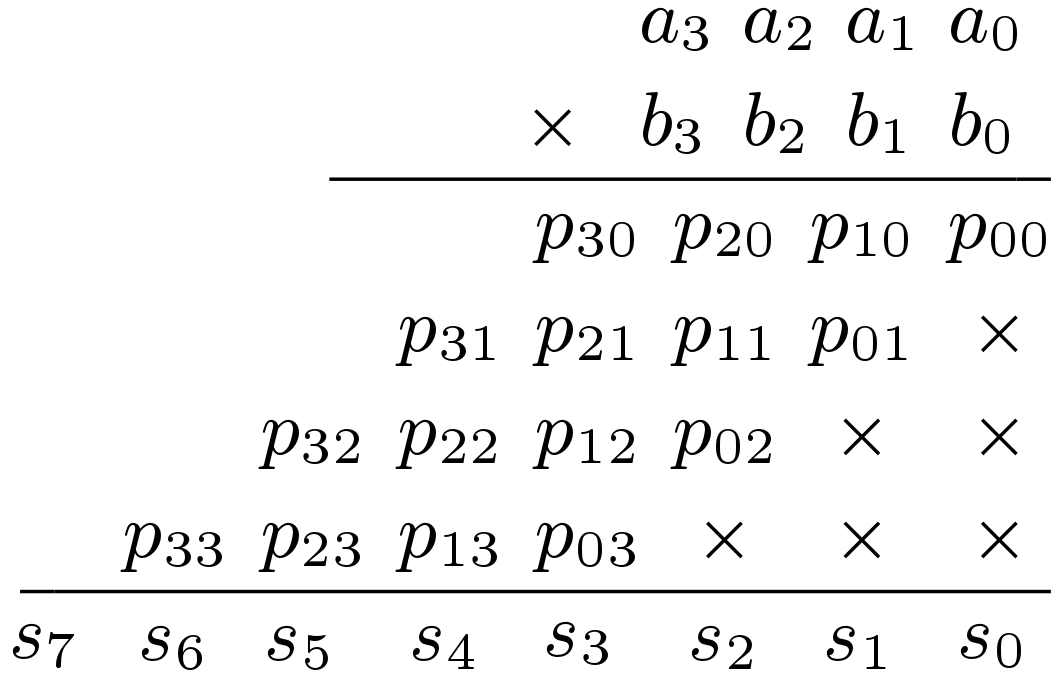
\includegraphics[width=\linewidth]{figs/EM-array_multiplier_unsigned.png}
    \end{minipage}
    }
    \subfigure[部分积的阵列累加电路]{
    \label{EM:Fig:array_multiplier_FA}
    \begin{minipage}[t]{0.48\linewidth}
    \centering
    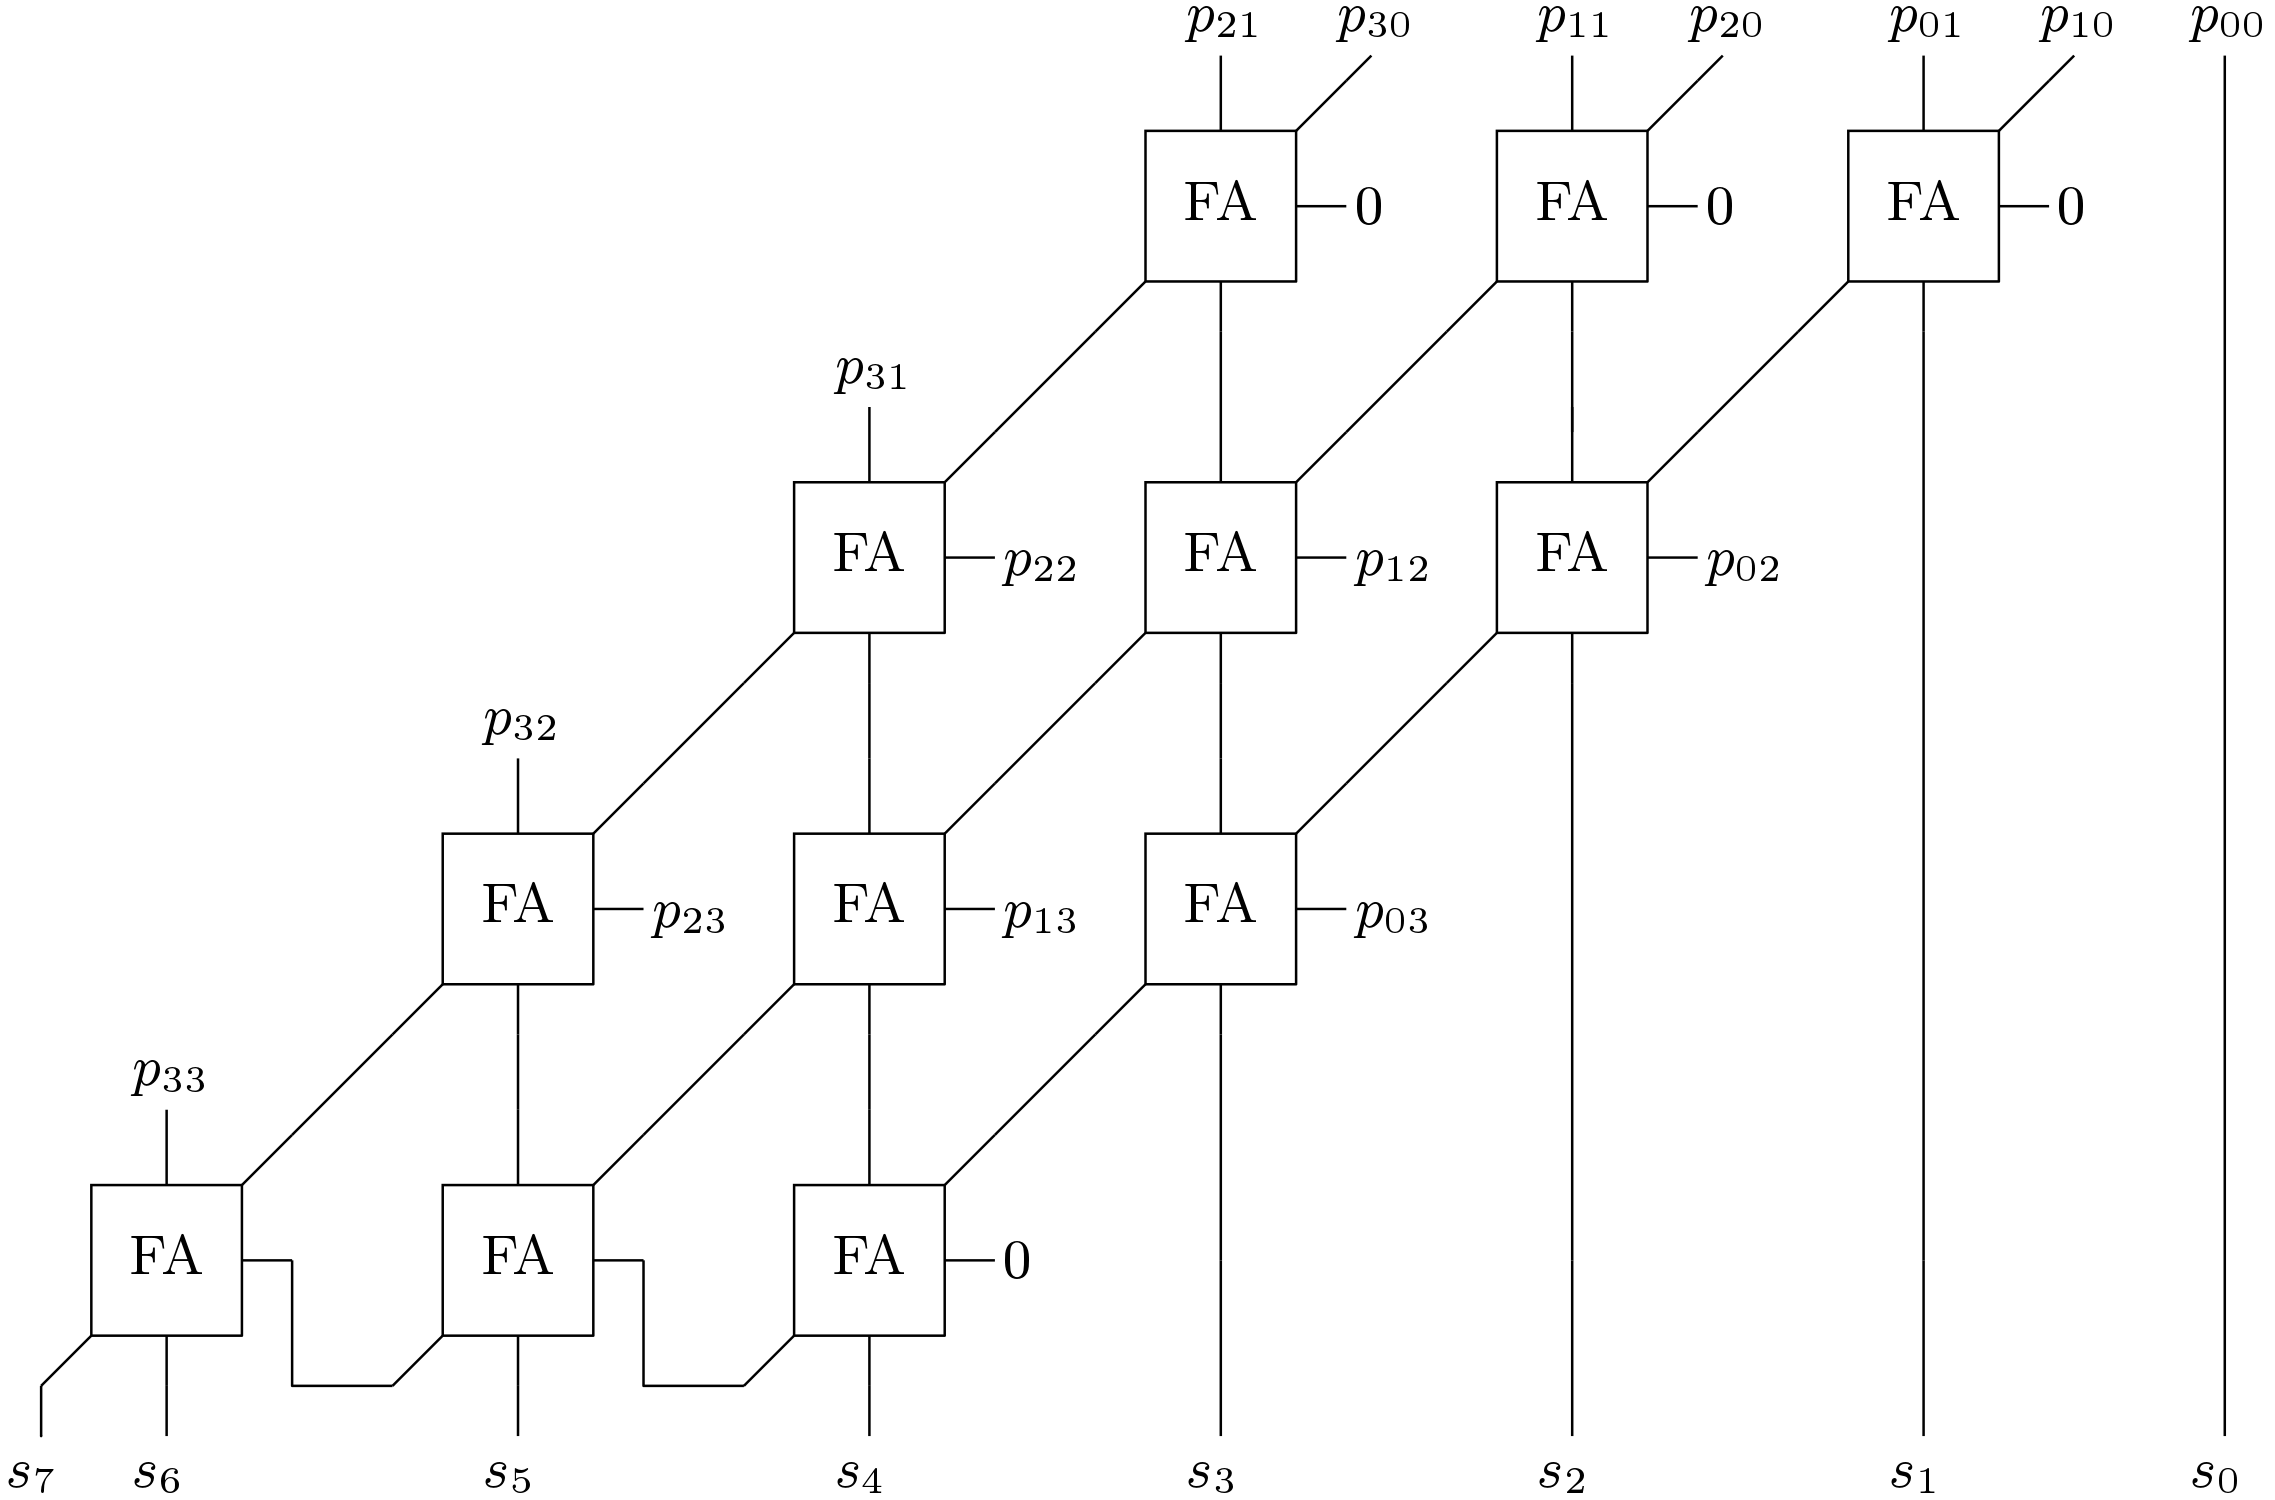
\includegraphics[width=\linewidth]{figs/EM-array_multiplier_FA.png}
    \end{minipage}
    }
\caption{$4\times4$无符号数乘法部分积及对应的阵列累加电路示意图}
\label{EM:Fig:array_multiplier}
\end{figure}

图\ref{EM:Fig:array_multiplier}展示了一个$4\times4$无符号数乘法部分积的生成及阵列累加电路示意图,部分积的移位操作通过布线即可完成,整个结构可以被很轻易的压缩成一个矩形,使得版图非常紧凑。阵列累加可以直接生成最终结果,并不需要最终相加这一步操作。然而,阵列累加结构中部分积的相加是通过逐位进位实现的,关键路径较长,性能较差。

\subsubsection{进位保留加法器}

进位保留加法器(Carry Save Adder, CSA)可以高效的对多个(通常是3个及以上)二进制数进行求和,通常用于乘法器中部分积的累加。在二进制中,两个或三个比特相加产生的进位不会超过1,基于此发现,CSA的基本思想是通过全加器将进位信号和求和信号保存下来,不断累加,直到将部分积压缩为两行,通过一个向量合并加法器得到最终结果。图\ref{EM:Fig:CSA}展示了一个4操作数8比特位宽,最后通过超前进位加法器进行向量合并的CSA结构图。
\begin{figure}[!htb]
    \centering
    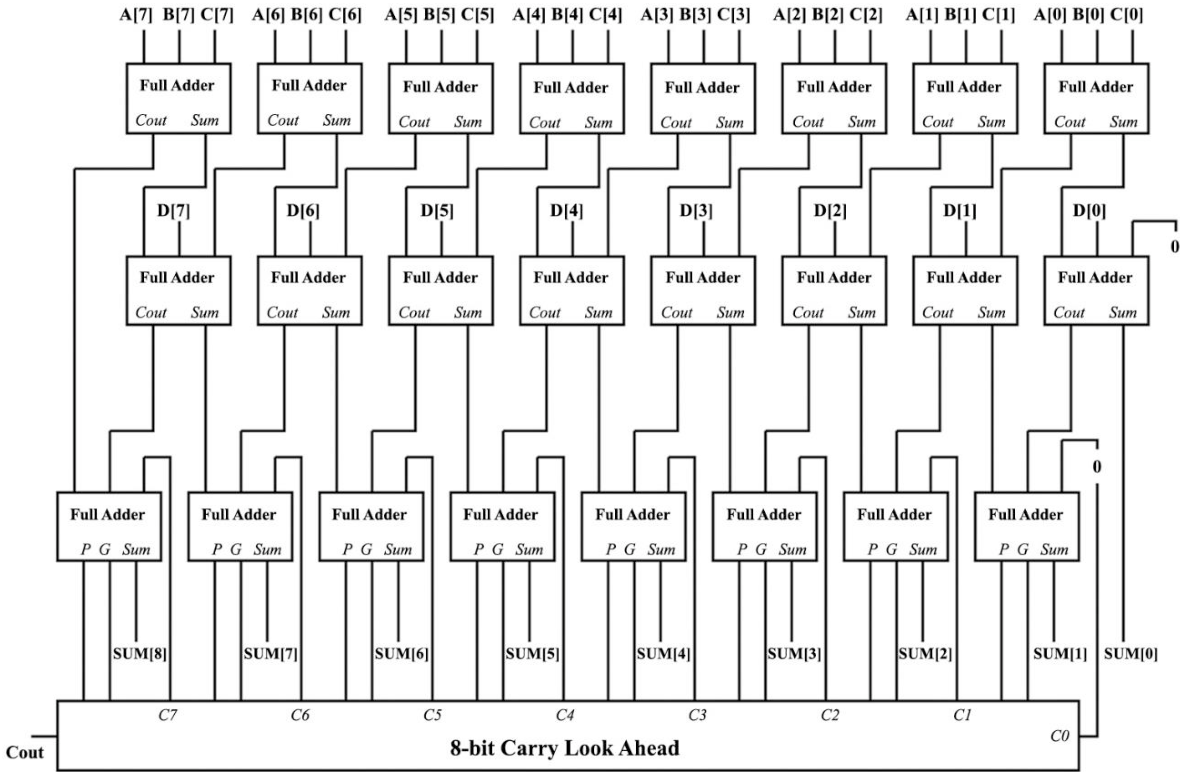
\includegraphics[width=0.85\textwidth]{figs/EM-CSA.png}
    \caption{4操作数8比特位宽,最后通过超前进位加法器相加的CSA结构图}
    \label{EM:Fig:CSA}
\end{figure}
从图中可以看到,4个8比特位宽的操作数经过两级全加器的运算变成了2个操作数,其中第一级全加器产生了$A$、$B$和$C$的进位及求和,之后和$D$一起被第二级全加器进行压缩,最后送给向量合并加法器进行求和。与阵列累加相比,CSA累加部分积的速度更快,性能更高。
注意这里的CSA并不会对操作数进行分组后并行累加,而是逐级累加\cite{数字集成电路_第十一章_设计运算功能块},这点与接下来讲的树形加法器有本质区别%
\IfStrEq{\Version}{Open}{%
    \footnote{\url{https://blog.csdn.net/qq_26707507/article/details/106146612}}。
}{。}

\subsubsection{树形加法器}

不论是阵列累加还是CSA累加本质上都是通过排列全加器实现的,全加器也可以安排为树形,这样既能减少累加电路所需的全加器的数量,还能降低关键路径延迟。树形加法器的实现可以看作是并行的进位保留加法器,累加效率更高。常见的树形加法器包括华莱士树\cite{EM:Wallace}和达达树\cite{EM:Dadda}。

(1)华莱士树 \label{华莱士树}

华莱士树(Wallace tree)加法器\cite{EM:Wallace}是由澳大利亚计算机科学家克里斯·华莱士(Christopher Stewart Wallace)于1964年设计的,被广泛用于乘法器中部分积的高效快速累加。其基本步骤如下:(a)假设所有部分积都是同时生成的,第一步是将部分积每3个分为一组(不足3个保持),并将每组部分积的个数通过全加器和半加器压缩为2个;(b)重复对部分积进行分组并压缩,直到只剩下两个部分积;(c)相加最后两个部分积得到最终结果。
\begin{figure}[!htb]
    \centering
    
\includegraphics[width=0.85\textwidth]{figs/EM-wallace.pdf}
    \caption{利用华莱士树加法器对$8 \times 8$无符号数乘法部分积进行累加的示意图}
    \label{EM:Fig:wallace}
\end{figure}
图\ref{EM:Fig:wallace}展示了一个利用华莱士树加法器对$8 \times 8$无符号数相乘产生的部分积进行累加的过程示意图,每个点表示一个比特,每个圈代表一个全加器或半加器(包含两个点的圈代表半加器,包含三个点的圈代表全加器),一共分组并压缩了4次,消耗了15个半加器和38个全加器,将8个部分积变成了2个部分积,改进的华莱士树方法能够使用更少的半加器,降低设计的复杂度\cite{EM:redeuce_wallace}。
与阵列累加方法和进位保留方法相比,华莱士树加法器的速度很快,且位宽越大越明显,但缺点是电路结构非常不规则,难以获得高质量的版图设计。全加器本质上是一个3:2压缩器,能够将乘法器中每组部分积的数目减少至三分之二,利用4:2甚至更高比例的压缩器,基于华莱士树方法可以得到性能更高的乘法器\cite{EM:wallace_42}。

(2)达达树

达达树(Dadda tree)加法器是由计算机科学家Luigi Dadda于1965年发明的一种树形加法结构\cite{EM:Dadda},与华莱士树方法类似,达达树也是采用全加器和半加器对部分积进行压缩,直到只剩下两个部分积。区别在于,Luigi Dadda对华莱士树进行了重构,在树的级数(深度)不变的情况下使用了数量更少的全加器和半加器,节省了硬件资源,但缺点是最后两个部分积的位宽可能会稍大。具体步骤如下%
\IfStrEq{\Version}{Open}{%
    \footnote{\url{https://en.wikipedia.org/wiki/Dadda_multiplier}}:
}{:}
\begin{itemize}
    \item 部分积的累加过程由一个正整数序列$d_j$来控制:$d_1=2$,$d_{j+1}=\lfloor 1.5 \rfloor d_j$,$\lfloor \ \rfloor$表示向下取整;
    \item 初始的$j$应尽可能大并满足$d_j < n$,$n$是乘数的位宽(部分积阵列的高度);
    \item $j$逐步递减,且任意$j$下对部分积阵列从最低权重按列开始遍历:(a)若列高度小于或等于$d_j$,跳过该列;(b)若列高度等于$d_j+1$,运用半加器对该列最上面的两个比特进行运算,产生进位及求和;(c)若列高度大于$d_j+1$,运用全加器对该列最上面的三个比特进行运算,产生进位及求和,并对该列重复(a)、(b)、(c)的操作;注意进位会增加相邻高权重列的高度;
    \item 累加结束时$j=1$,$d_j=2$(部分积只有两行),之后使用一个向量合并加法器求得最终结果。
\end{itemize}

图\ref{EM:Fig:dadda}展示了一个运用达达树对$8 \times 8$无符号数乘法生成的部分积进行压缩的过程示意图,该树的深度与图\ref{EM:Fig:wallace}中的华莱士树的深度相同,但使用了更少的全加器和半加器:达达树使用了35个全加器、7个半加器,华莱士树使用了38个全加器、15个半加器。
\begin{figure}[!htb]
    \centering
    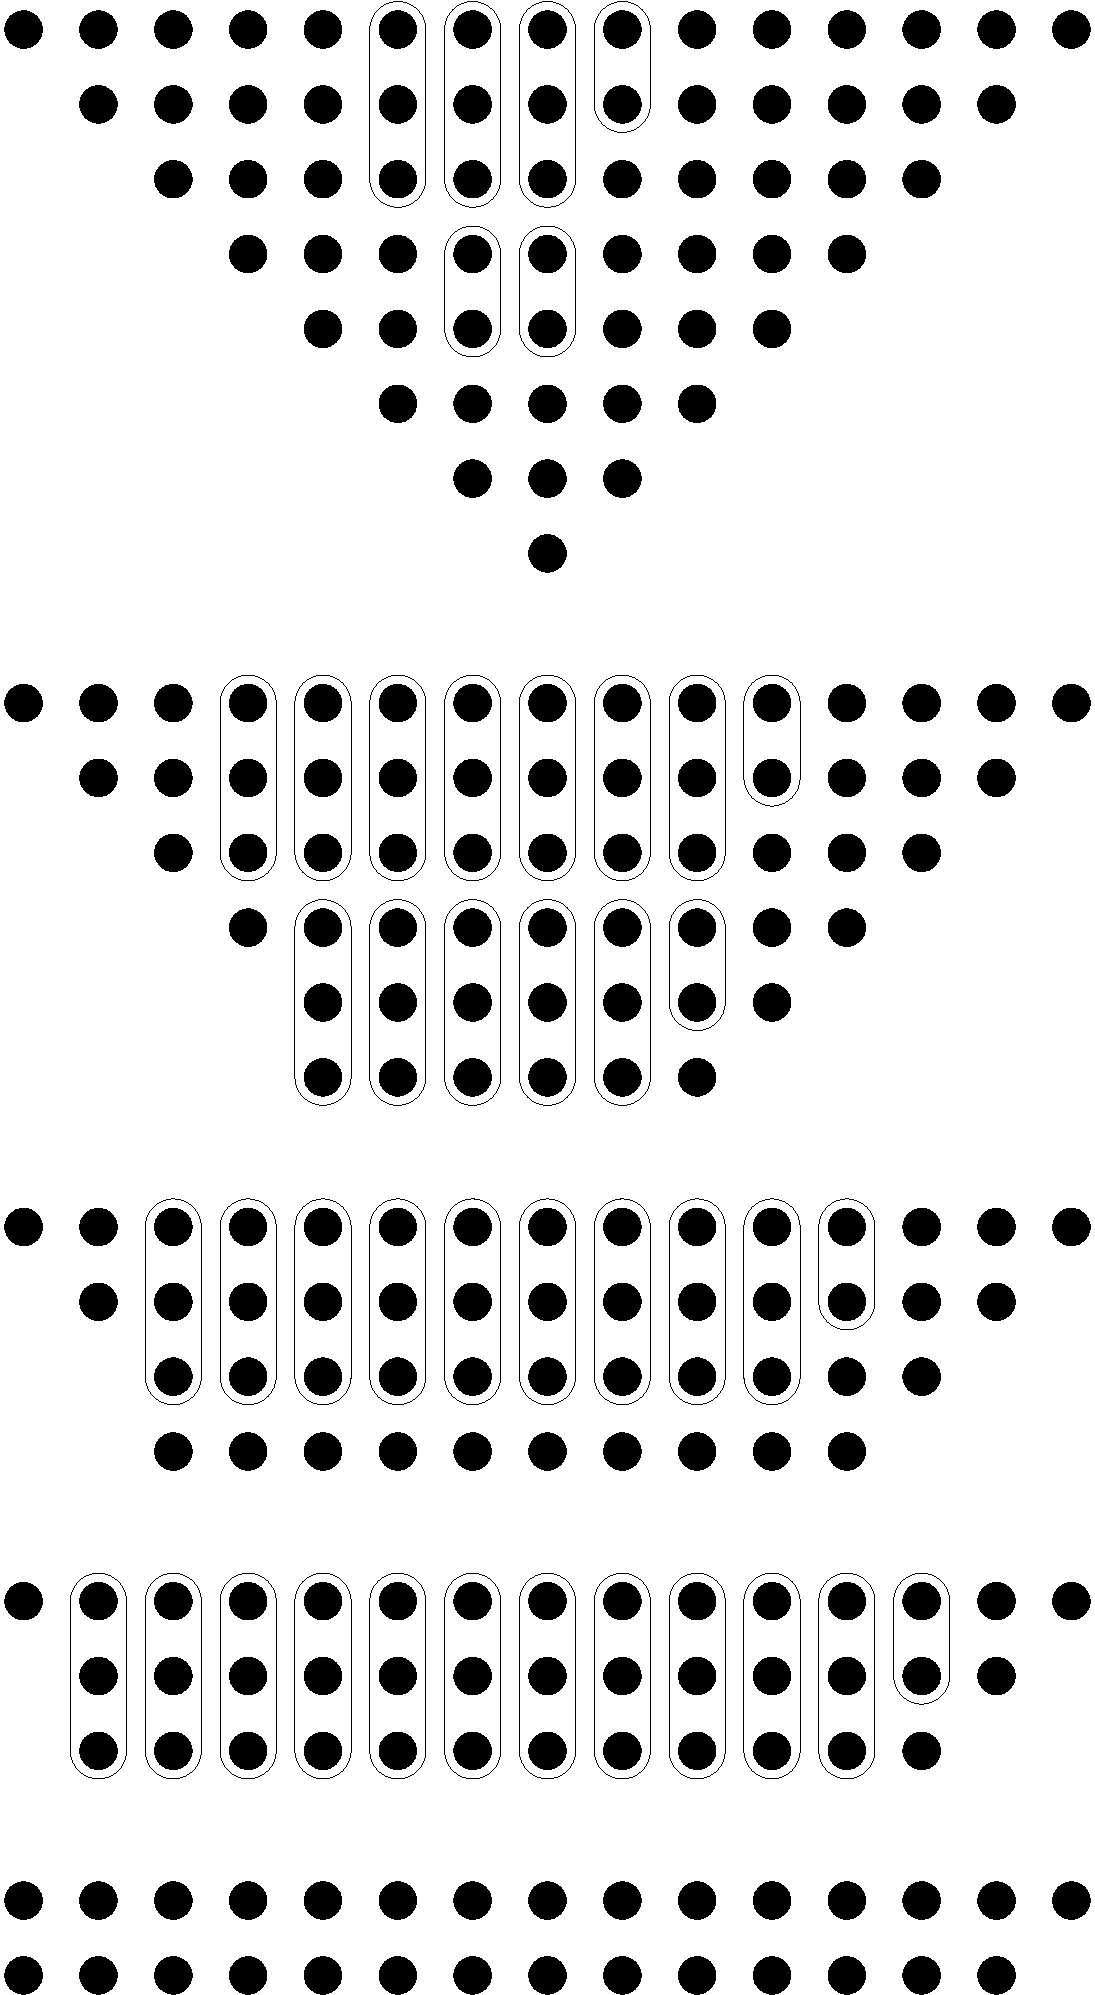
\includegraphics[width=0.7\textwidth]{figs/EM-dadda.pdf}
    \caption{利用达达树加法器对$8 \times 8$无符号数乘法部分积进行累加的示意图}
    \label{EM:Fig:dadda}
\end{figure}

\subsection{最终相加}

除了阵列累加方式以外,进位保存加法器、树形加法器等高速的部分积累加电路最后会产生两个部分积,需要一个向量合并加法器(Vector-Merging Adder, VMA)进行最终运算,目前常见的VMA有以下几种结构:

\subsubsection{行波进位加法器}

行波进位加法器(Ripple-Carry Adder, RCA)又被称为逐级进位加法器,是由一系列全加器级联而成,优点是面积小、占用资源少,缺点是速度慢、效率低。在最好情况下,任何位宽的RCA都不需要传递进位信号也可以得到正确结果;但在最坏情况下,得到最终结果的延迟会随着位宽的增加而线性增大,从而限制了系统的运算速度。

\subsubsection{超前进位加法器}

当加法器的位宽较大时,由于RCA在最坏情况下每一级全加器的计算必须等待前一级的进位输出,导致其关键路径较长,效率较低,超前进位加法器(Carry-Lookahead Adder)的思想是并行计算每一级全加器的进位输出,本质上是数学公式推导的结果,原理如下:

假设RCA中第$i$级全加器的输入为$a_i$、$b_i$、$c_{i}$,进位输出为$c_{i+1}$,设$p_i = a_i \oplus b_i$,$g_i = a_i b_i$,有:
\begin{equation}
\begin{aligned}
    c_{i+1} = & \ a_i b_i + c_i(a_i \oplus b_i) \\
    = & \ g_i + c_i p_i
\end{aligned}
\label{EM:Eq:CLA}
\end{equation}
若$p_i=1$,则$g_i =0$,$c_{i+1}=c_i$,若$p_i=0$,则$c_{i+1}=g_i$,因此$p_i$和$g_i$分别被称为第$i$级加法器的传播信号和生成信号。
对$c_{i}, c_{i-1},c_{i-2},\cdots,c_{1}$使用式\eqref{EM:Eq:CLA},可将$c_{i+1}$的求解转换为输入数的逻辑操作(假设$c_0=0$),避免了RCA中的进位依赖问题,实现了效率的提升。与RCA相比,CLA的关键路径短,速度快,但在加法器位宽较大时,CLA中高位的进位输出表达式涉及的变量较多,存在较大扇入扇出的问题。同时,组合逻辑电路的输入信号过多也会引起竞争冒险(Race hazard),产生毛刺(Glitch),影响系统的稳定性。所以在加法器的位宽较大时,要想利用CLA提高进位效率,通常会先对操作数进行划分,对每个部分实行CLA,CLA之间再通过级联或嵌套等方式进行连接%
\IfStrEq{\Version}{Open}{%
    \footnote{\url{https://zhuanlan.zhihu.com/p/378267920}},
}{,}
以避免大输入位宽逻辑门的产生。其中,采用级联对各CLA块之间进行连接的方式被称为分块CLA,采用嵌套对各CLA块之间进行连接的方式被称为分级CLA。
灵活地对操作数进行划分并嵌套,能够得到许多不同的CLA结构,可在面积和速度之间进行权衡,存在一套能够简洁表示各种分级超前进位结构的符号体系,具体内容在后面的并行前缀加法器中详细讲述。
最后需要注意的是,基于CLA方法实现的加法器的面积和复杂度通常会比同位宽的RCA大。

\subsubsection{进位旁路加法器}

基于式\eqref{EM:Eq:CLA}可以看到,一个$n$位RCA的最坏情况发生在$p_{n-1}, p_{n-2}, \cdots, p_0$均为1的时候(即$p_{n-1} p_{n-2} \cdots p_0=1$),此时$g_{n-1}, g_{n-2}, \cdots, g_0$均为0,式\eqref{EM:Eq:CLA}变为:
\begin{equation}
    c_{i+1} =  c_i
\label{EM:Eq:CSKA_prop}
\end{equation}
进位旁路加法器(Carry-Skip Adder,为了与进位保存加法器区分,这里缩写为CSKA,也叫Carry-bypass adder)的思想便是加速该情况下进位链的传播。一个$n$位的CSKA包括一个$n$位的RCA、一个$n$位的多输入与门(AND)、以及一个二选一的多路选择器(Multiplexer, MUX)。图\ref{EM:Fig:CSKA_4bit}展示了一个4比特CSKA的结构图,$p_0 \sim p_3$信号通过与门连接到MUX上作为选择信号,当$p_0 p_1 p_2 p_3=1$时,$c_0$通过MUX直接输出,中间的RCA被旁路掉,大大减少了延迟。
\begin{figure}[!htb]
    \centering
    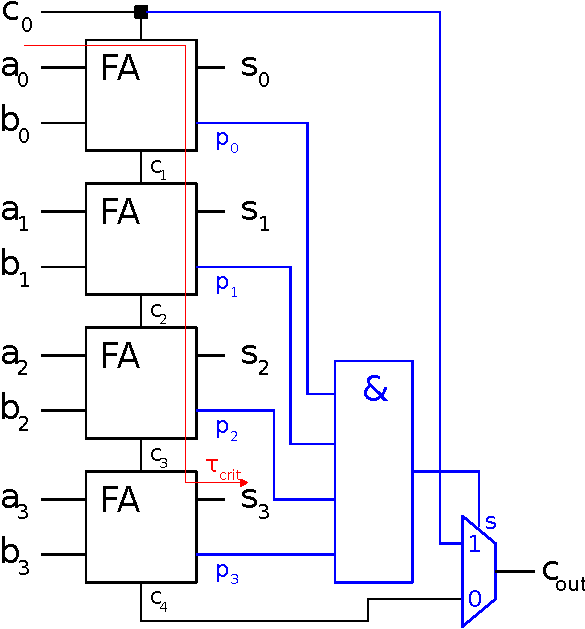
\includegraphics[width=0.4\textwidth]{figs/EM-CSKA_4Bit.pdf}
    \caption{一个4比特CSKA的结构示意图,FA代表全加器}
\label{EM:Fig:CSKA_4bit}
\end{figure}

但是,与RCA相比,CSKA并没有明显的性能改进(如图\ref{EM:Fig:CSKA_4bit}中的关键路径$\tau_{\text{crit}}$同样需要经过4个全加器)。因此,当位宽较大时,采用分块CSKA(Block CSKA)的办法才能取得较为显著的速度增益。若一个$n$比特的分块CSKA有$m$块CSKA,每块CSKA的位宽均为$\dfrac{n}{m}$,则该分块CSKA被称为固定大小分块CSKA%
\IfStrEq{\Version}{Open}{%
    \footnote{\url{https://en.wikipedia.org/wiki/Carry-skip_adder}}。
}{。}
\begin{figure}[!htb]
    \centering
    \includegraphics[width=\textwidth]{figs/EM-CSKA_16Bit.pdf}
    \caption{一个固定大小分块CSKA的例子:通过级联4个4比特CSKA实现16比特加法}
\label{EM:Fig:CSKA_16bit}
\end{figure}

图\ref{EM:Fig:CSKA_16bit}展示了一个通过级联4个4比特CSKA实现的16比特固定大小分块CSKA加法器的结构图,其关键路径(红色线条$\text{T}_{\text{critical}}$)延迟包括头尾两个4比特RCA的延迟和中间两个旁路逻辑中MUX的延迟。从静态时序分析(Static Timing Analysis, STA)的角度看,图\ref{EM:Fig:CSKA_16bit}的关键路径延迟比一个16比特的RCA更差,但STA得到的关键路径是伪路径,电路实际运行过程中并不会发生。固定大小分块CSKA真实的关键路径可通过以下过程来理解:输入同时到来后,每块CSKA很快地被确定为是否处于旁路状态;之后所有的CSKA同时计算,假设首块CSKA没有被旁路,那么当首块CSKA的进位输出得到后,后面所有的CSKA要么处于旁路状态、要么也已计算完毕。
因此固定大小分块CSKA的最坏情况是,进位信号需要通过首尾两个RCA和中间全部处于旁路状态的CSKA中的MUX。通过调整块的大小和层级,分块CSKA的性能可得到进一步地优化。
最后需要注意的是,与其他快速加法器如CLA不同,分块CSKA的性能仅在输入是某些情况下会获得提高,即速度的提高是概率性的。

\subsubsection{进位选择加法器}

另一种避免出现RCA中最坏情况下逐级进位的方法是预先考虑进位输入的两种可能的值(0和1),并提前计算针对这两种可能性的结果,一旦进位输入的值确定,正确的结果可以通过一个简单的MUX选出,这一设想的实现被称为进位选择加法器(Carry-Select Adder,为了与进位保存加法器区分,这里缩写为CSEA)。CSEA通常只包括RCA和MUX,一个4比特位宽的CSEA的结构如图\ref{EM:Fig:CSEA_basic}所示,由于一个RCA的进位为0,而另一个RCA的进位为1,因此可通过实际进位输入决定哪个RCA的结果作为输出,与同位宽的RCA相比,除了MUX以外,CSEA消耗了两倍数量的全加器,是面积换性能的典型代表。
\begin{figure}[!htb]
    \centering
    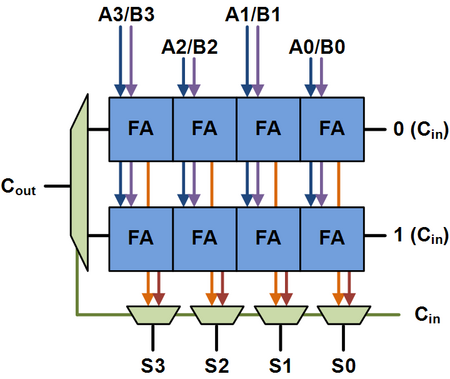
\includegraphics[width=0.5\textwidth]{figs/EM-CSEA_basic.png}
    \caption{一个4比特CSEA的结构图,FA代表全加器}
\label{EM:Fig:CSEA_basic}
\end{figure}

完整的CSEA加法器需要对多个小的CSEA进行级联,并额外引入一个RCA。若每个小CSEA的位宽相同,该加法器被称为线性(Linear)CSEA;若每个小CSEA的位宽不同,该加法器被称为可变大小(Variable-sized)CSEA,一种特殊的可变大小CSEA是平方根(Square-root) CSEA。

(1)线性进位选择加法器

\begin{figure}[!htb]
    \centering
    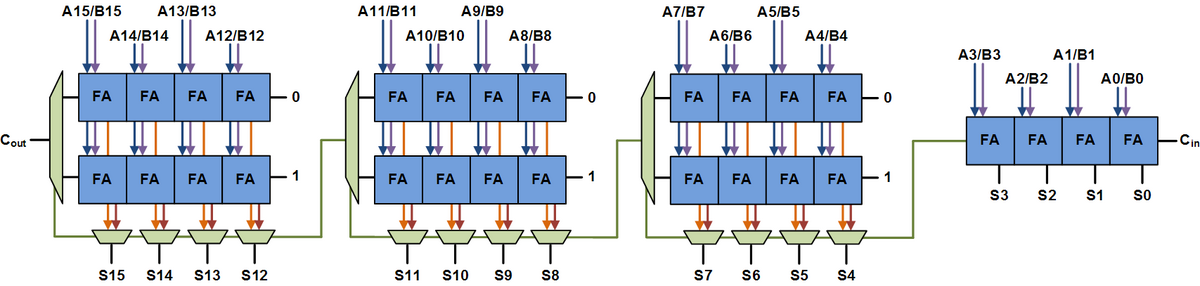
\includegraphics[width=\textwidth]{figs/EM-CSEA_linear.png}
    \caption{一个16比特线性进位选择加法器示意图}
\label{EM:Fig:CSEA_linear}
\end{figure}

图\ref{EM:Fig:CSEA_linear}展示了一个16比特线性CSEA的结构示意图,该加法器由一个4比特RCA和三个4比特CSEA组成,其关键路径包括初始的4比特RCA和后续三个MUX,可通过以下过程理解:当初始的RCA计算完成时,后面所有的小CSEA中的RCA均计算完成,只需等待真正的进位输入信号进行选择即可。
通常来讲,对于一个$n$比特线性CSEA,每个小CSEA的位宽取$\lfloor \sqrt n \rfloor$性能最好%
\IfStrEq{\Version}{Open}{%
    \footnote{\url{https://en.wikipedia.org/wiki/Carry-select_adder}},
}{,}
这里$\lfloor \ \rfloor$代表向下取整。

(2)平方根进位选择加法器

若级联的每个小CSEA的位宽不同,且数值大小从低位到高位依次为$2$、$3$、$4$、$\cdots$,初始RCA的位宽为2,则该可变大小CSEA被称为平方根CSEA,如图\ref{EM:Fig:CSEA_square}所示,关键路径为初始的2位宽的RCA和后续的3个MUX。
\begin{figure}[!htb]
    \centering
    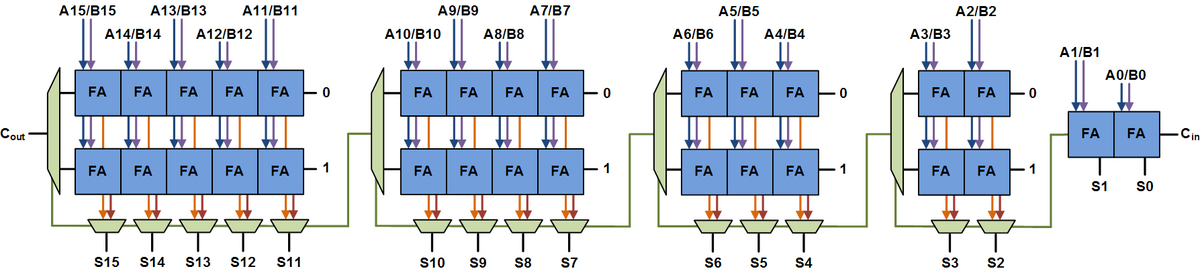
\includegraphics[width=\textwidth]{figs/EM-CSEA_square.png}
    \caption{16比特平方根进位选择加法器示意图}
\label{EM:Fig:CSEA_square}
\end{figure}
平方根CSEA假设全加器和MUX的延迟相等,避免了线性CSEA中高位CSEA计算完成后等待进位输入信号选择的缺点,不论位宽多大,其关键路径总是初始的2位宽RCA加上后续的MUX,与线性CSEA相比取得了显著的性能提升。不过,一般情况下全加器和MUX的延迟并不相等,因此需要根据实际情况决定使用哪种结构的CSEA。

\subsubsection{并行前缀加法器\cite{EM:book_Computer_Arithmetic}}

由式\eqref{EM:Eq:CLA}可得:
\begin{align}
    c_{i+1} = & \ \textcolor{blue}{g_i} +\textcolor{blue}{p_i} c_i \notag \\
          = & \ g_i + p_i \textcolor{red}{(g_{i-1} + p_{i-1} c_{i-1})} \notag \\
          = & \ \textcolor{blue}{(g_i + p_i g_{i-1})} + \textcolor{blue}{(p_i p_{i-1})} c_{i-1} \notag \\
          = & \ (g_i + p_i g_{i-1}) + (p_i p_{i-1}) \textcolor{red}{(g_{i-2} + p_{i-2} c_{i-2})} \notag \\
          = & \ \textcolor{blue}{(g_i + p_i g_{i-1} + p_i p_{i-1} g_{i-2})} + \textcolor{blue}{(p_i p_{i-1} p_{i-2})} c_{i-2} \notag \\
          = & \ \cdots
\label{EM:Eq:PPA_CLA}
\end{align}
设$i$、$j$均是整数且$0 \le i < j$,将$p$和$g$的定义从单比特拓展到连续的多比特,有:
\begin{align}
    & g_{[i,j]} =  g_j + p_j g_{j-1} + p_j p_{j-1} g_{j-2} + \cdots + (p_j p_{j-1} p_{j-2} \cdots p_{i+1}) g_i \notag \\
    & p_{[i,j]} = p_j p_{j-1} p_{j-2} \cdots p_i \notag \\
    & c_{j+1} = g_{[i,j]} + p_{[i,j]} c_i
\label{PPA_multi_bit_gp}
\end{align}
即对加法块$[i,j]$来讲同样存在进位的生成信号$g_{[i,j]}$和传播信号$p_{[i,j]}$,考虑到两者总是成对出现,可将其简写为二元对$(g_{[i,j]},p_{[i,j]})$。对两个相邻、部分重叠或完全重叠的加法块,$(g_{[i,j]},p_{[i,j]})$有如下性质:

相邻:假设$k$是整数且$i<k<j$,则块$[i,k-1]$与块$[k,j]$相邻,满足:
\begin{align}
    g_{[i,j]} = & \ g_{[k,j]} + g_{[i,k-1]} p_{[k,j]} \notag \\
    p_{[i,j]} = & \ p_{[i,k-1]} p_{[k,j]}
\label{EM:Eq:PPA_相邻}
\end{align}

部分重叠:假设$h$是整数且$i<k<h<j$,则块$[i,h]$与块$[k,j]$重叠,满足:
\begin{align}
    g_{[i,j]} = & \ g_{[k,j]} + g_{[i,h]} p_{[k,j]} \notag \\
    p_{[i,j]} = & \ p_{[i,h]} p_{[k,j]}
    \label{EM:Eq:PPA_部分重叠}
\end{align}

完全重叠,满足:
\begin{align}
    g_{[i,j]} = & \ g_{[i,j]} + g_{[i,j]} p_{[i,j]} \notag \\
    p_{[i,j]} = & \ p_{[i,j]} p_{[i,j]}
    \label{EM:Eq:PPA_完全重叠}
\end{align}

\begin{figure}[!b]
    \centering
    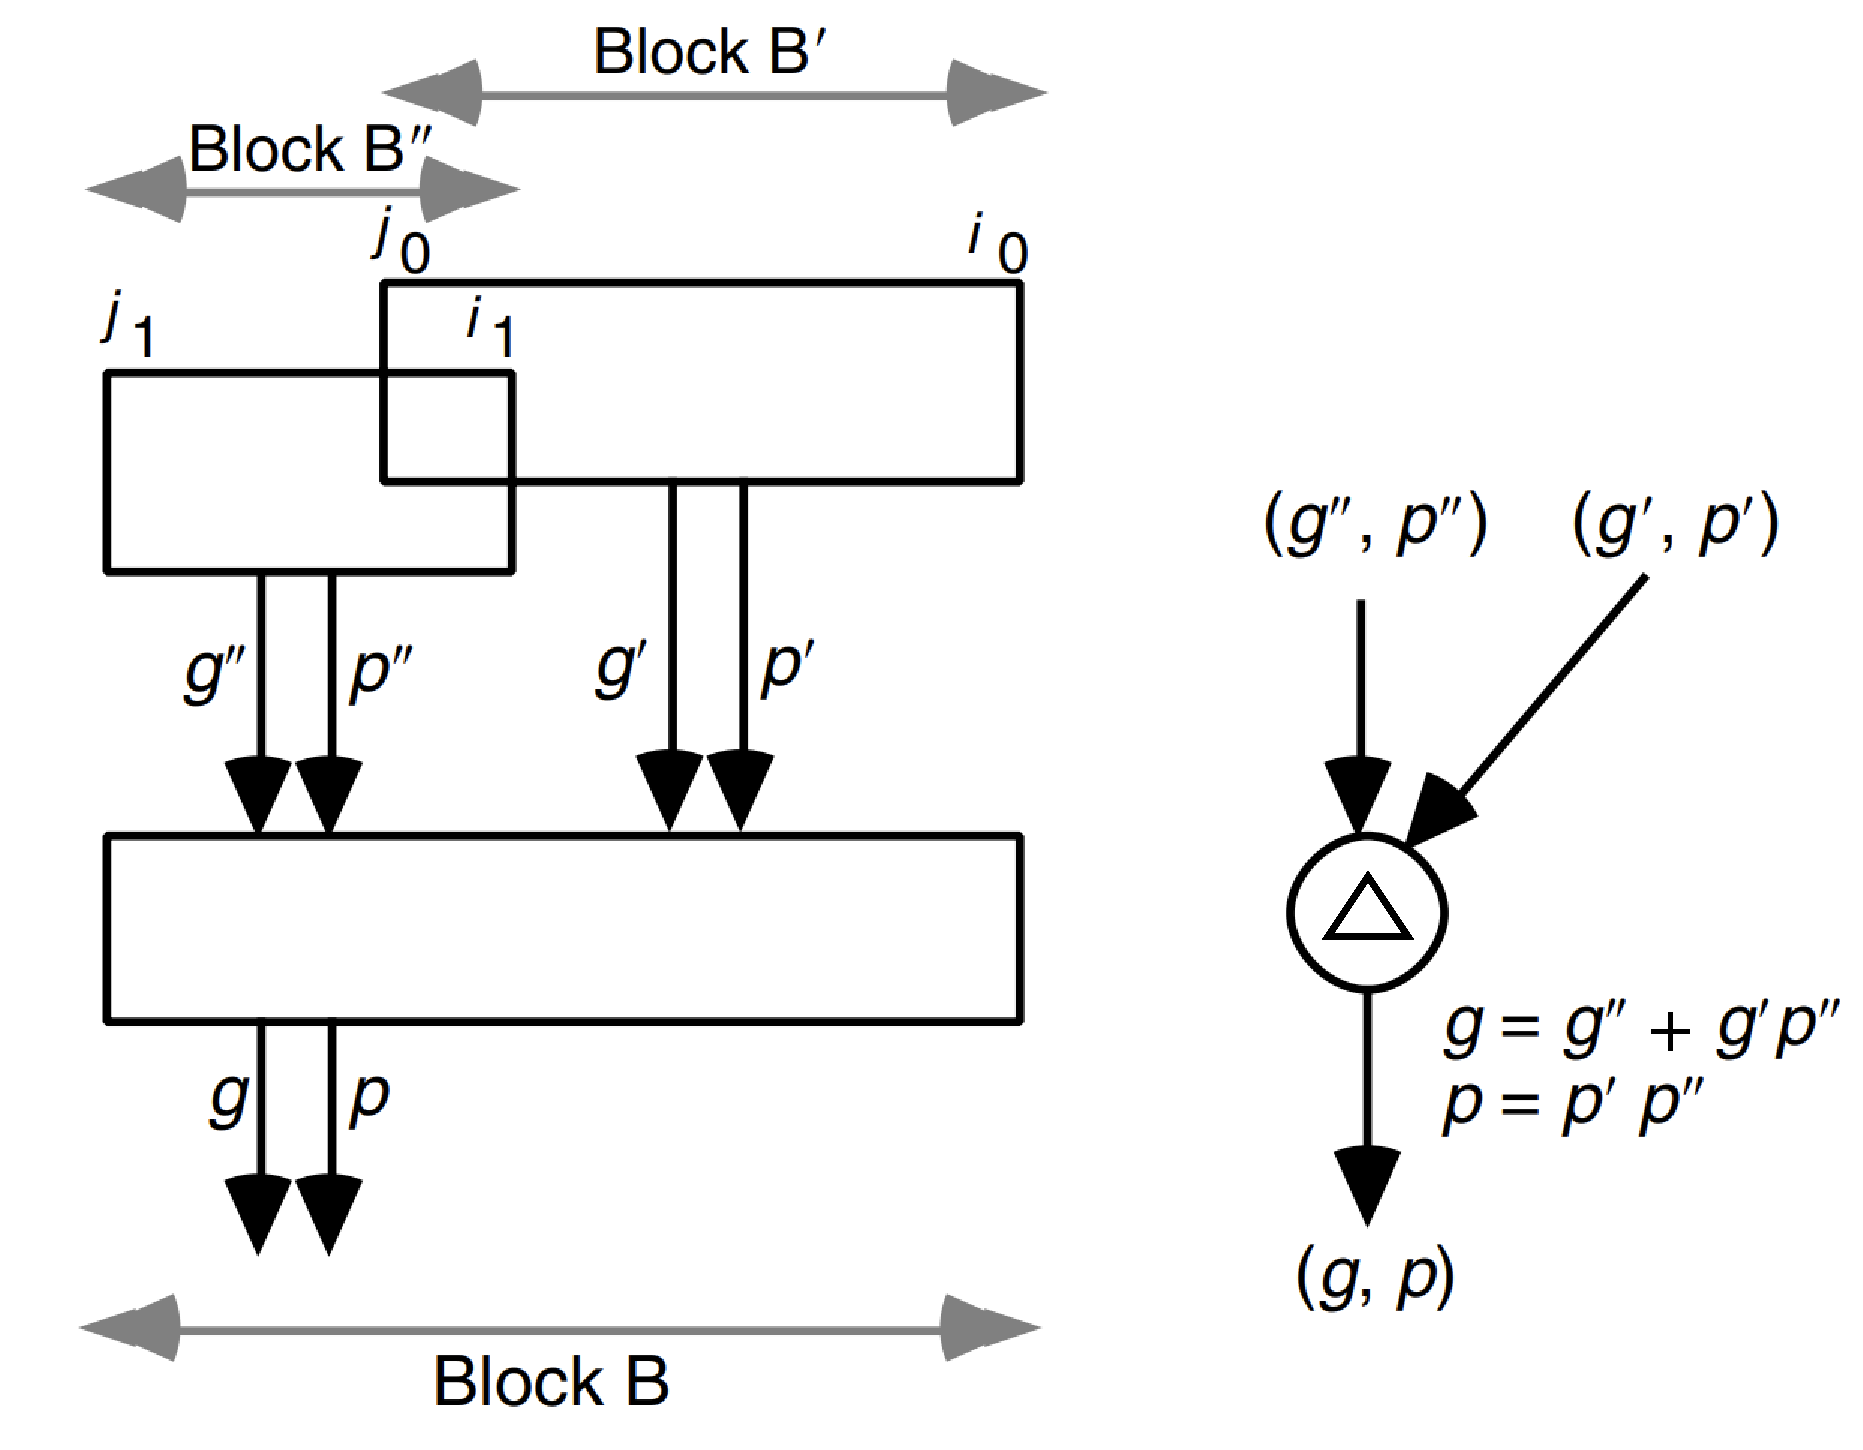
\includegraphics[width=0.6\textwidth]{figs/EM-PPA_BB.pdf}
    \caption{合并两个相邻或部分重叠的加法块$B \prime$、$B \prime \prime$的进位信号}
\label{EM:Fig:PPA_BB}
\end{figure}
如图\ref{EM:Fig:PPA_BB}所示,假设两个加法块$B \prime$和$B \prime \prime$相邻或重叠,则可以通过合并两对进位信号$(g \prime, p \prime)$和$(g \prime \prime, p \prime \prime)$来得到块$B$的进位信号$(g,p)$,假设该合并操作符号为$\triangle$,有:
\begin{equation}
    (g,p) = (g \prime, p \prime) \triangle (g \prime \prime, p \prime \prime)
\end{equation}
其中
\begin{equation}
    g = \ g \prime \prime + g \prime p \prime\prime , \ \ \ \ p = \ p \prime p \prime \prime
\end{equation}
注意$\triangle$满足结合律,不满足交换律:
\begin{align}
    ( \ (g \prime, p \prime) \triangle (g \prime \prime, p \prime \prime) \ ) \triangle (g \prime \prime \prime, p \prime \prime \prime) & \equiv (g \prime, p \prime) \triangle ( \ (g \prime \prime, p \prime \prime) \triangle (g \prime \prime \prime, p \prime \prime \prime) \ ) \notag \\
    (g \prime, p \prime) \triangle (g \prime \prime, p \prime \prime) & \not\equiv (g \prime \prime, p \prime \prime) \triangle (g \prime, p \prime)
\end{align}
这里假设块$B \prime \prime \prime$与块$B \prime \prime$相邻或重叠,进位信号为$(g \prime \prime \prime, p \prime \prime \prime)$。

基于此,可以定性地描述出进位问题:
假设加法器的位宽为$n$,给定$(g_0,p_0)$、$(g_1,p_1)$、$(g_2,p_2)$、$\cdots$、$(g_{n-1},p_{n-1})$,通过并行地计算
\begin{equation}
    (g_0,p_0) \triangle (g_1,p_1) \triangle (g_2,p_2) \triangle \cdots \triangle (g_{n-1},p_{n-1})
\end{equation}
能够得到所有的$(g_{[0,0]},p_{[0,0]})$、$(g_{[0,1]},p_{[0,1]})$、$(g_{[0,2]},p_{[0,2]})$、$\cdots$、$(g_{[0,n-1]},p_{[0,n-1]})$,即$c_1$、$c_2$、$c_3$、$\cdots$、$c_n$,且不同的并行方法对应不同的进位逻辑硬件实现,具有不同的面积和性能,称为并行前缀进位(Parallel Prefix Carry, PPC),得到的加法器被称为并行前缀加法器。
\begin{figure}[!htb]
    \centering
    \subfigure[超前进位加法器CLA的PPC树状图]{
    \label{EM:Fig:PPC_CLA}
    \begin{minipage}[t]{0.48\linewidth}
    \centering
    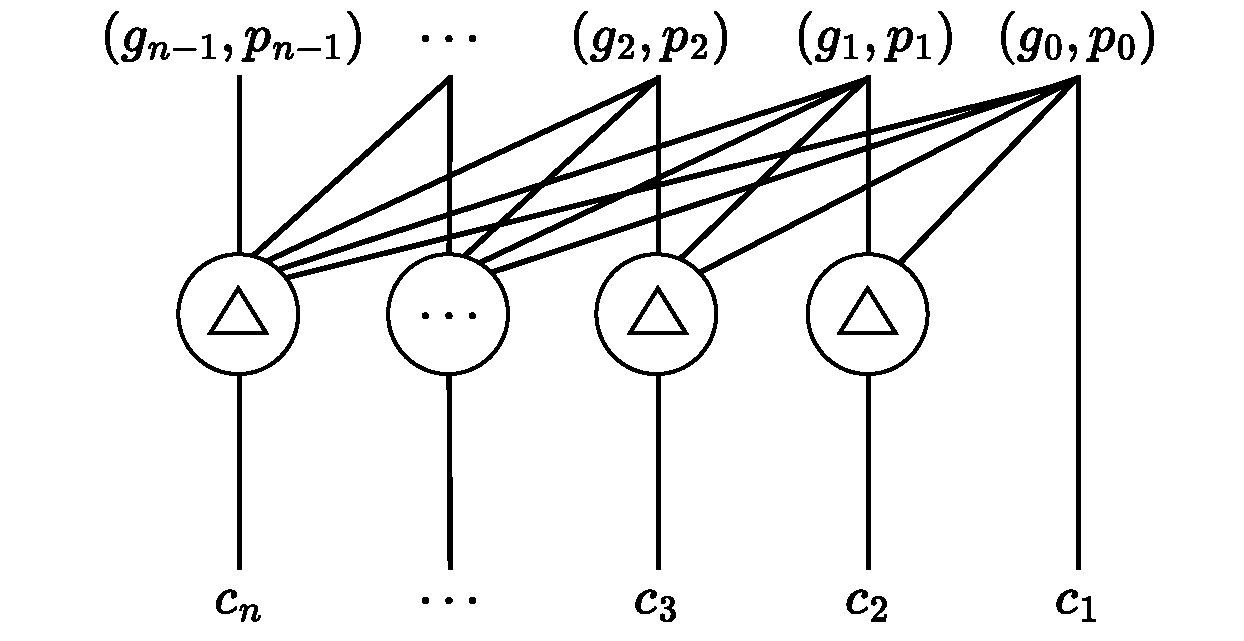
\includegraphics[width=\linewidth]{figs/EM-PPC_CLA.pdf}
    \end{minipage}
    }
    \subfigure[行波进位加法器RCA的PPC树状图]{
    \label{EM:Fig:PPC_RCA}
    \begin{minipage}[t]{0.48\linewidth}
    \centering
    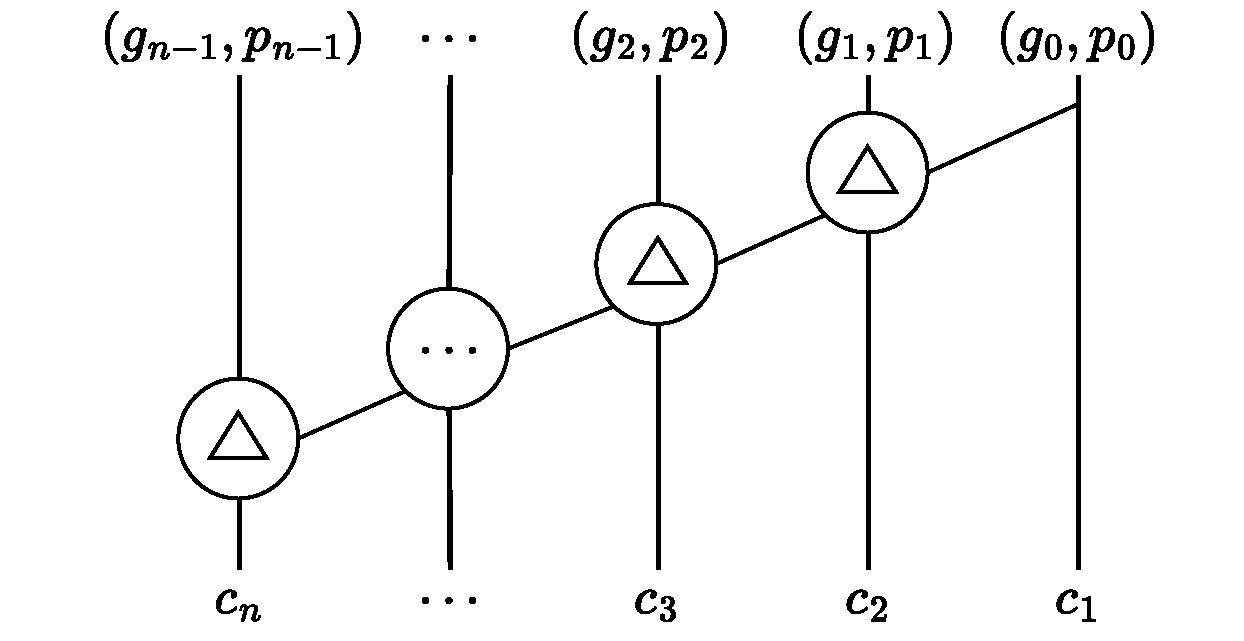
\includegraphics[width=\linewidth]{figs/EM-PPC_RCA.pdf}
    \end{minipage}
    }
\caption{标准CLA和标准RCA的PPC树状图}
\label{EM:Fig:PPC_CLA_RCA}
\end{figure}
PPC可由树状图进行表示,图\ref{EM:Fig:PPC_CLA_RCA}展示了标准超前进位加法器CLA和标准行波进位加法器RCA的PPC树状图。可以看到,CLA的PPC树状图只有一级,关键路径短,但计算量大;CLA的PPC树状图有$n$级,关键路径长,但使用了大量的中间节点,计算量小。因此,并行前缀加法器的核心在于如何对面积和延迟进行权衡,这为并行前缀加法器的设计带来了非常大的灵活性\cite{EM:PPA_PPT}:
比如1960年的Sklansky加法器\cite{EM:Sklansky_adder},特点是级数少、扇出高;
1973年的Kogge-Stone加法器\cite{EM:Kogge-Stone_adder},优点是逻辑级数和扇出都非常小,缺点是节点数量非常多,布线拥塞度高;
1980年的Ladner-Fisher加法器\cite{EM:Ladner-Fisher_adder},其结构与Sklansky加法器\cite{EM:Sklansky_adder}一致,原因是Ladner-Fischer形式化了进位问题的求解,Sklansky加法器是其中一种方案;
1982年的Brent-Kung加法器\cite{EM:Brent-Kung_adder},优点是扇出非常小,节点也较少,缺点是逻辑级数较多,即通过增加额外的逻辑级数来缓解扇出压力;
1987年的Han-Carlson加法器\cite{EM:Han-Carlson_adder},混合了Brent-Kung结构和Kogge-Stone结构,更有利于硬件实现;
1999年Knowles提出可以从逻辑深度、布线拥塞度和面积三个方面对进位网络的设计进行权衡\cite{EM:S-Knowles_adder};
2003年Harris提出了一个有趣的3-D结构图来对已有的并行前缀加法器进行分类\cite{EM:Harris_3-D},同时提出了一个新的进位结构;其余的前缀加法器包括Ling型加法器\cite{EM:Ling_adder}和具有多扇入节点的Beaumont-Smith加法器\cite{EM:Beaumont-Smith_adder}。
现代EDA(Electronic Design Automation)综合工具通常会根据用户的约束来实现具有不同并行前缀结构的加法器。由于大位宽下并行前缀网络的搜索空间巨大,英伟达利用强化学习的方法设计出了面积更小、速度更快的加法器\cite{EM:PrefixRL};也有工作在观察到EDA流程中逻辑综合和物理综合结果的不统一后\cite{EM:PPA_Pareto},通过图神经网络进行优化\cite{EM:PPA_GNN}。

\section{对数乘法器} \label{对数乘法器}

1962年,John N. Mitchell提出了一个相当有趣的算法\cite{EM:mitchell}:在二进制下,可以通过加法来近似得到两个无符号非零定点数的乘积,最大误差不超过$\dfrac{1}{9}$,且编程实现非常简洁,原理如下:

% 设$m=0$,由式\eqref{EM:Eq:unsigned_fixed_Decimal}得两个$n$比特二进制无符号正整数$X$和$Y$的十进制值:, 

对于式\eqref{EM:Eq:unsigned_fixed_Binary},假设$R=2$、$m=0$,两个$n$比特二进制无符号整数$X$和$Y$:
\begin{equation}
    X = x_{n-1} x_{n-2} x_{n-3} \cdots x_1 x_0 \ \ \ \ \ \ \ \
    Y = y_{n-1} y_{n-2} y_{n-3} \cdots y_1 y_0 
\label{EM:Eq:mitchell_XY_binary}
\end{equation}
若$X$和$Y$均非零(正整数),有:
\begin{align}
    x_{n-1} + x_{n-2} + x_{n-3} + \cdots + x_1 + x_0 = 1 \notag \\
    y_{n-1} + y_{n-2} + y_{n-3} + \cdots + y_1 + y_0 = 1
\end{align}
式中$+$表示逻辑或,则$X$和$Y$的十进制值为:
\begin{align}
    V(X) = \sum_{i=0}^{k_X} x_i 2^i \ \ \ \ \ \ \ \ \ \ \ \ \ \ \ 
    V(Y) = \sum_{i=0}^{k_Y} y_i 2^i
\end{align}
其中$k_X$和$k_Y$分别代表$X$和$Y$中最高位的1的权重值\cite{AC:AM:TOSAM},$X$和$Y$取不同值时$k_X$和$k_Y$的值也不同,乘积$P$的十进制值:
\begin{align}
    V(P) = & \ V(X)V(Y) \notag \\
    = & \ \sum_{i=0}^{k_X} x_i 2^i \times \sum_{i=0}^{k_Y} y_i 2^i \notag \\
    = & \ 2^{k_X} ( \ 1 + \sum_{i=0}^{k_X - 1} x_i 2^{i-k_X} \ ) \times 2^{k_Y} ( \ 1 + \sum_{i=0}^{k_Y - 1} y_i 2^{i-k_Y} \ ) \notag \\
    = & \ 2^{k_X + k_Y} ( \ 1 + \sum_{i=0}^{k_X - 1} x_i 2^{i-k_X} \ ) ( \ 1 +  \sum_{i=0}^{k_Y - 1} y_i 2^{i-k_Y}\ ) \notag \\
    = & \ 2^{k_X + k_Y} ( \ 1 + x^{\prime} \ ) ( \ 1 + y^{\prime} \ )
\label{EM:Eq:mitchell_P_orig}
\end{align}
其中
\begin{equation}
    x^{\prime} = \sum_{i=0}^{k_X - 1} x_i 2^{i-k_X} \ \ \ \ \ \ \ \
    y^{\prime} = \sum_{i=0}^{k_Y - 1} y_i 2^{i-k_Y}
\end{equation}
则:
\begin{equation}
    \log_2 (V(P)) = k_X + k_Y + \log_2 (1+x^{\prime}) + \log_2 (1+y^{\prime})
\label{EM:Eq:mitchell_log_P}
\end{equation}
易知$x, y \in [0,1)$,在这里,Mitchell做了一个相当果断而美妙的近似,那就是利用$\log_2 (1+x^{\prime}) \approx x^{\prime}$和$\log_2 (1+y^{\prime}) \approx y^{\prime}$将式\eqref{EM:Eq:mitchell_log_P}变为:
\begin{equation}
    \log_2 (V(P)) \approx k_X + k_Y + x^{\prime} + y^{\prime}
\label{EM:Eq:mitchell_log_P_2}
\end{equation}
则乘积$P$:
\begin{equation}
    V(P) \approx 2^{(k_X + k_Y)} \cdot 2^{(x^{\prime} + y^{\prime})}
\label{EM:Eq:mitchell_P_middle}
\end{equation}
这里再做一次近似:
\begin{equation}
    x^{\prime} + y^{\prime} \approx \left\{
    \begin{aligned}
        \ & \log_2 (1 + x^{\prime} + y^{\prime}) , & \ \ x^{\prime} + y^{\prime} < 1, \\
        \ & 1 + \log_2 (x^{\prime} + y^{\prime}), & \ \ x^{\prime} + y^{\prime} \ge 1.
    \end{aligned}
    \right.
\end{equation}
则式\eqref{EM:Eq:mitchell_P_middle}变为:
\begin{equation}
    V(P) \approx \left\{
    \begin{aligned}
        \ & 2^{(k_X + k_Y)} (1 + x^{\prime} + y^{\prime}) , & \ \ x^{\prime} + y^{\prime} < 1, \\
        \ & 2^{(k_X + k_Y + 1)} (x^{\prime} + y^{\prime}), & \ \ x^{\prime} + y^{\prime} \ge 1.
    \end{aligned}
    \right.
\label{EM:Eq:mitchell_P_final}
\end{equation}
式\eqref{EM:Eq:mitchell_P_final}即为Mitchell对数乘法器的最终形式,只需要加法、移位和检测电路即可完成两数相乘,可以证明Mitchell算法的最大误差不超过精确值的$\dfrac{1}{9}$。

在C++中,Mitchell算法有一个非常简单的实现%
\IfStrEq{\Version}{Open}{%
    \footnote{\url{https://kexue.fm/archives/7991}},
}{,}
单精度(Single precision)浮点数Mitchell算法的代码如算法\ref{EM:Alg:mitchell_Cpp}所示\cite{DNN:mitchell_Training},原理如下:

\begin{algorithm}[!]
    float int mitchell\_mul (const float a, const float b) \{ \\
    \ \ \ \ \ \ \ \ int c = *(int*)\&a + *(int*)\&b - 0x3f800000; \\
    \ \ \ \ \ \ \ \ return *(float*)\&c; \\
    \}
\caption{Mitchell算法在C++中的简单实现}
\label{EM:Alg:mitchell_Cpp}
\end{algorithm}

C++中int类型通常是32位,同时IEEE 754标准规定采用32个比特表示单精度浮点数,如图\ref{EM:Fig:mitchell_IEEE754}所示,其中最高位表示正负,之后8位表示科学计数法的指数,最后23位表示科学计数法的小数,注意指数部分需要加上偏移量127。对于两个单精度浮点数a和b,*(int*)\&a和*(int*)\&b其实就是把a和b对应的二进制表示拿出来,当作普通的int类型将两者相加,对应式\eqref{EM:Eq:mitchell_log_P_2},这时指数部分还多出一个偏移量,所以要减去这个偏移量,由于偏移量是127,并且后面还有23位,所以要减去常数$127×2^{23}$(十六进制为0x3f800000),最后将结果恢复成单精度浮点数。对双精度(Double precision)浮点数来说,在引入64比特位宽的long int类型和正确的偏移量($1023 \times 2^{52} = \text{0x3feffffb9f6e8000}$)之后,算法\ref{EM:Alg:mitchell_Cpp}同样适用(已验证)。

\begin{figure}[!htb]
    \centering
    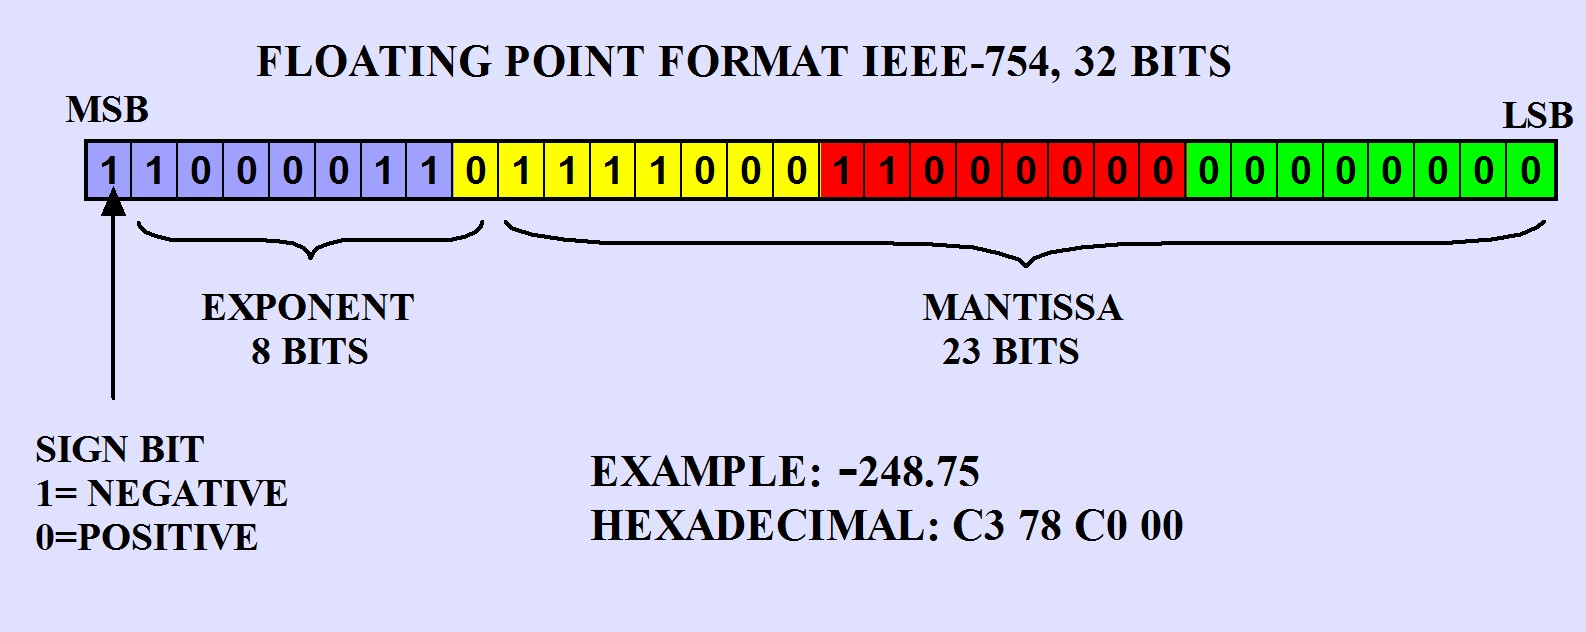
\includegraphics[width=0.8\linewidth]{figs/EM-mitchell_IEEE754.jpg}
    \caption{IEEE 754单精度浮点数标准}
    \label{EM:Fig:mitchell_IEEE754}
\end{figure}

Mitchell算法能够将乘法近似转化为加法实现,这对含有大量乘法并对误差有容忍性的神经网络应用带来了计算量优化的可能,比如文献\cite{DNN:mitchell_Training}在“ImageNet+ResNet50”中直接将神经网络中的精确乘法转换为Mitchell乘法,准确率只有轻微的下降,类似的工作也有多篇\cite{AC:AM:mitchell_aspdac2018,AC:AM:mitchell_tc2019}。

\section{近似电路的误差指标} \label{近似电路的误差指标}

近似电路通常是指近似的算术运算单元,如加法器、减法器、乘法器、除法器等。这些近似模块在计算中可能会产生误差,用来衡量误差的最基本的两个指标分别是误差率(Error Rate, ER)和误差距离(Error Distance, ED)\cite{AC:Arith:survey_hanjie}。ER表示产生错误结果的概率,ED代表近似结果和精确结果之间的算术差异。假设在某输入下近似电路的结果是$M \prime$,精确电路的结果是$M$,那么该输入下误差距离为:
\begin{equation}
    ED = | M′−M |
\label{AC:Arith:ED}
\end{equation}
相对误差距离(Relative ED, RED)表示近似结果与准确结果之间的相对算术差异,定义为:
\begin{equation}
    RED = \dfrac{ED}{M}
\label{AC:Arith:RED}
\end{equation}
ED和RED是衡量近似电路在某输入下误差的两个重要指标。

当考虑所有的输入情况时,可由平均误差距离(Mean ED, MED)和平均相对误差距离(Mean RED, MRED)来衡量近似电路和精确电路之间的整体算术差异,MED和MRED被定义为:
\begin{align}
    & MED = \sum _{i=1}^{N} ED_{i} \cdot P(ED_{i}) \label{AC:Arith:MED} \\
    & MRED = \sum _{i=1}^{N} RED_{i} \cdot P(RED_{i}) \label{AC:Arith:MRED}
\end{align}
其中$N$是所有输入情况的总数,$ED_{i}$和$RED_{i}$分别代表第$i$种输入情况下的误差距离ED和相对误差距离RED,$P(ED_{i})$和$P(RED_{i})$分别代表$ED_{i}$和$RED_{i}$发生的概率,即输入取第$i$种情况的概率。MED也被叫做平均绝对误差(Mean Absolute Error, MAE)。
归一化平均误差距离(Normalized MED, NMED)被定义为MED除以精确电路在所有可能输入情况下的最大值,常被用来比较同一近似设计方法在不同输入位宽下的误差表现。

均方误差(Mean Squared Error, MSE)和均方根误差(Root MSE, RMSE)也被广泛用于衡量近似电路和精确电路之间的整体算术差异,它们被定义为:
\begin{align}
    & MSE = \sum _{i=1}^{N}ED_{i}^{2}\cdot P(ED_{i}) \label{AC:Arith:MSE} \\
    & RMSE = \sqrt {MSE} \label{AC:Arith:RMSE}
\end{align}
另外,平均误差被定义为所有可能输入情况下$M \prime - M$的平均值,归一化平均误差被定义为平均误差除以精确电路在所有可能输入情况下的最大值。最后,最坏情况误差(Worst Case Error, WCE)反映了所有可能输入情况下ED的最大值。

以上提到的近似电路的误差指标均适用于近似乘法器。

\section{基于功能近似的近似乘法器相关工作}

从电路实现的底层结构上看,基于功能近似\cite{AC:ALS:survey}实现的近似乘法器设计方法可分为面向ASIC和FPGA两类,下面分别进行介绍。

\subsection{4类现有的ASIC近似乘法器设计方法}

(1)手工设计(Manual design)

手动化简乘法器的电路或门级网表的方法被称为手工设计方法,这种方法的优点在于通常能在不同位宽的乘法器之前迁移,缺点是费时费力,且无法灵活地根据应用的错误容忍程度进行调整,效果较差。

较为经典的一篇有关手工设计近似乘法器的工作是由Kulkarni等人\cite{AC:AM:KMap}于2011年发表的,他们观察到$2 \times 2$精确乘法器只有在输入是$3 \times 3$的时候才需要4个比特对输出进行表示,于是修改了卡诺图(Karnaugh map),将$3 \times 3 = 9$变为了$3 \times 3 = 7$,输出从原先需要4个比特减少到了3个比特,乘法器的门数降低了37.5\%,面积消耗更小。与精确的$2 \times 2$乘法器相比,该近似乘法器在16种可能的输入情况中,只有一种情况输出是错误的,误差率ER是$\dfrac{1}{16}$,由式\eqref{AC:Arith:ED}得输入为3$\times$3时的误差距离ED为$|7 − 9| = 2$。经过EDA软件评估,近似后的$2 \times 2$乘法器的面积相比精确版本减少了一半,并且拥有更短的关键路径。同时,由于近似后乘法器的开关电容更小,在相同工作频率下的动态功耗也更低。大位宽的乘法器可通过拆分的方法由近似的$2 \times 2$乘法器搭建起来,且搭建时可让高位输入保持精确乘法来降低误差。

文献\cite{AC:AM:CR}对行波进位加法器RCA中的全加器进行了重新设计,将进位输入信号替换成了前一级全加器的非进位输入,使进位链最多只能传播两位,优化了关键路径,降低了计算延迟,同时将截断进位链产生的误差保存了下来。优化后的全加器被排列成树形用于乘法器中部分积的累加及最终相加,并在最终相加后根据需要引入不同等级的误差补偿,提高乘法器的精度。精确的误差补偿需要考虑所有全加器保存的误差并相加,为了降低设计复杂度,仅考虑最高几位全加器保存的误差,通过或(OR)操作运算后加到最终的输出上。
图\ref{AC:AM:Fig:CR_app_adder}代表论文提出的考虑两级输入的近似全加器电路图,其中$S_i$和$E_i$分别代表求和输出与保存的误差。图\ref{AC:AM:Fig:CR_app_mul}展示了论文提出的基于近似全加器单元设计的近似乘法器的结构示意图,其中A1-A7代表树形的近似全加器阵列,一方面对部分积进行累加,一方面保留产生的误差,最后的补偿步骤选择最高4位全加器的结果进行运算。需要注意的是,因为保存的误差是通过或操作运算之后相加到结果上,所以即使考虑所有全加器保存的误差也无法将误差率降到0(正确的做法不是或运算而是相加)。
\begin{figure}[!htb]
    \centering
    \subfigure[考虑两级输入的近似全加器单元]{
    \label{AC:AM:Fig:CR_app_adder}
    \begin{minipage}[t]{0.3\linewidth}
    \centering
    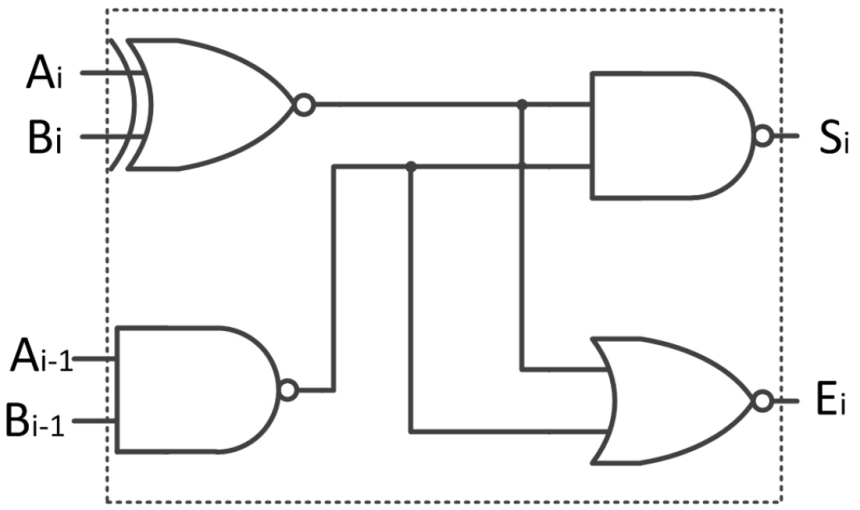
\includegraphics[width=\linewidth]{figs/AC-AM-CR_app_adder.png}
    \end{minipage}
    }
    \subfigure[提出的带有误差补偿模块的近似乘法器示意图]{
    \label{AC:AM:Fig:CR_app_mul}
    \begin{minipage}[t]{0.66\linewidth}
    \centering
    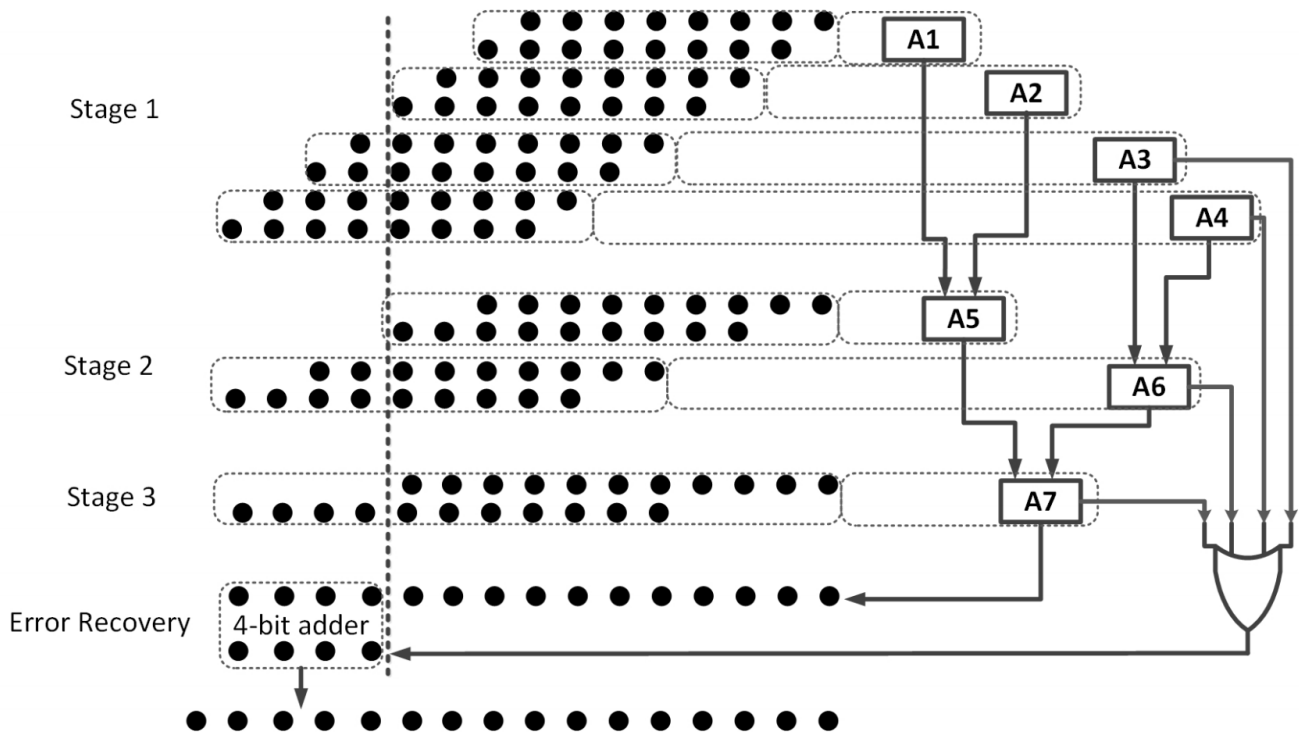
\includegraphics[width=\linewidth]{figs/AC-AM-CR_app_mul.png}
    \end{minipage}
    }
\caption{近似全加器单元和近似乘法器结构示意图}
\end{figure}

文献\cite{AC:AM:SDLC}在部分积生成后、累加前,先通过逻辑或(OR)操作有选择地对部分积进行了一次压缩,大大降低了部分积阵列的规模,减轻了后续的累加压力。除了2输入的或操作之外,更大输入的或操作也可以被使用,好处是部分积规模下降的更多,坏处是引入的误差更大。图\ref{AC:AM:Fig:SDLC_OR3}展示了利用3输入或门对部分积阵列进行压缩的过程:首先对部分积进行分组,每3个部分积一组,不足3个的可保持或使用更小输入的或门,同时避免操作高位部分积以减少误差,压缩后的部分积个数由8个减少为3个,降低了62.5\%。该论文提出的方法适用于不同位宽的乘法器,通过Synopsys Design Compiler综合工具对基于此方法设计的128比特位宽的近似乘法器进行评估发现,与精确乘法器相比,面积减少了45\%,关键路径减少了65\%。
\begin{figure}[!htb]
    \centering
    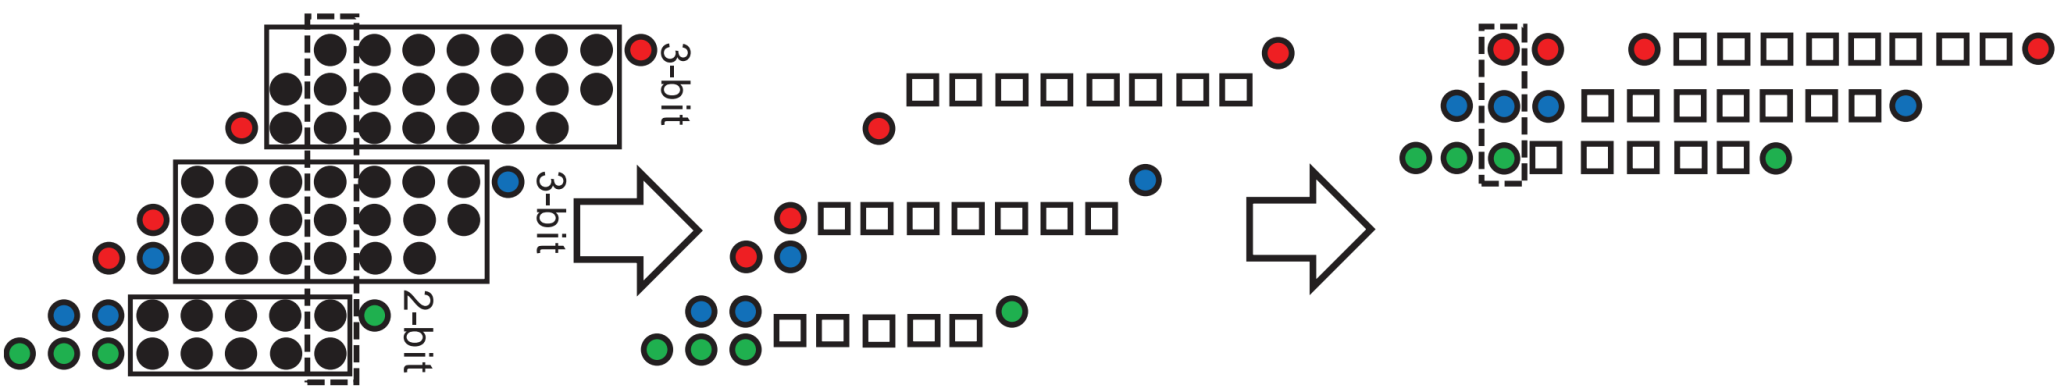
\includegraphics[width=\textwidth]{figs/AC-AM-SDLC_OR3.png}
    \caption{利用3输入或门对部分积阵列进行压缩}
\label{AC:AM:Fig:SDLC_OR3}
\end{figure}

文献\cite{AC:AM:DRUM}提出了一个用于两个无符号数相乘的动态无偏可配置乘法器DRUM,其基本思想是通过动态识别乘数和被乘数中权重最大的1的位置、挑选出以该位置开头的几个连续比特并对尾部数据进行四舍五入之后,利用一个小位宽的乘法器完成核心运算。整个电路包括检测器、四舍五入编码器、小位宽乘法器以及最后的移位器,可通过配置小乘法器的位宽来实现不同的精度。同时,该乘法器是无偏的,即平均误差为0(见\ref{近似电路的误差指标}有关平均误差的定义);该乘法器也是对称的,即对任意输入,交换乘数和被乘数后结果一致,没有极性。图\ref{AC:AM:Fig:DRUM_example}展示了DRUM计算过程的一个示例,在对操作数中挑出的部分比特四舍五入并执行乘法后,通过移位操作得到最终的结果。
\begin{figure}[!htb]
    \centering
    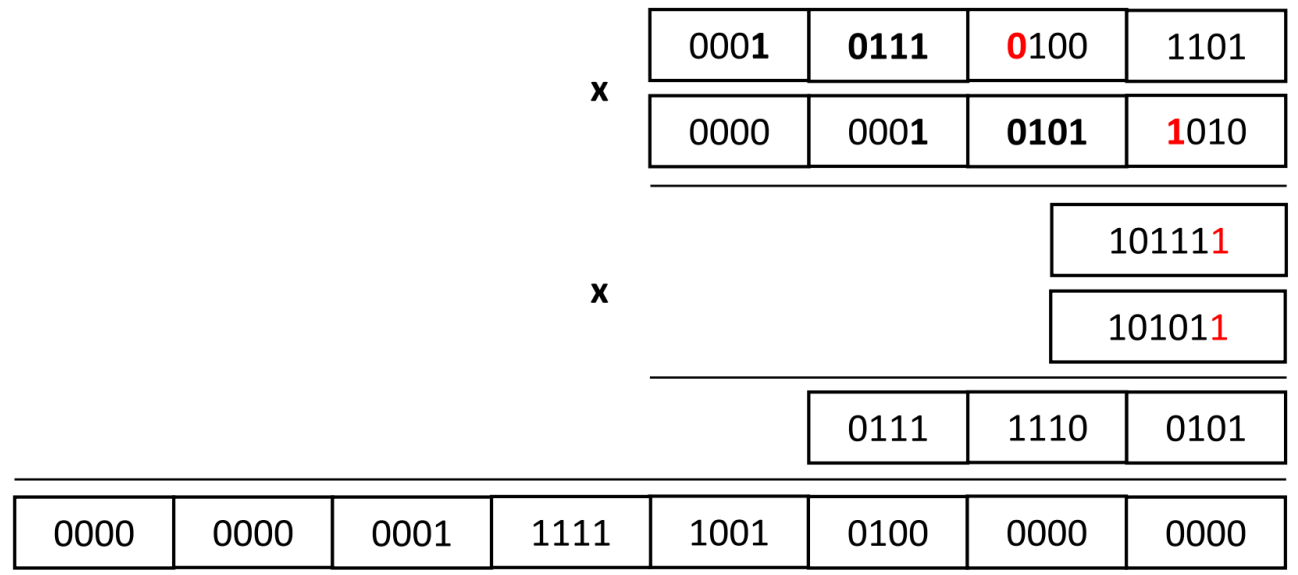
\includegraphics[width=0.7\textwidth]{figs/AC-AM-DRUM_example.png}
    \caption{DRUM计算过程的一个示例}
\label{AC:AM:Fig:DRUM_example}
\end{figure}

文献\cite{AC:AM:TOSAM}对式\eqref{EM:Eq:mitchell_P_orig}进行了变形:
\begin{align}
    V(P) = & \ 2^{k_X + k_Y} ( \ 1 + x^{\prime} \ ) ( \ 1 + y^{\prime} \ ) \notag \\
         = & \ 2^{k_X + k_Y} ( \ 1 + x^{\prime} \cdot y^{\prime} + x^{\prime} + y^{\prime} \ ) \notag \\
         \approx & \ 2^{k_X + k_Y} ( \ 1 + x^{\prime}_{App} y^{\prime}_{App} + x^{\prime}_T + y^{\prime}_T \ )
\label{AC:AM:Eq:TOSAM}
\end{align}
其中,$x^{\prime}_{App}$、$y^{\prime}_{App}$、$x^{\prime}_T$、$y^{\prime}_T$均是操作数中的部分比特,但与DRUM相比没有对尾部数据进行四舍五入而是直接丢弃,这样原始乘法被转换成了一个小位宽乘法和两个加法,减少了电路面积。同时,
$x^{\prime}_{App}$、$x^{\prime}_T$(或$y^{\prime}_{App}$、$y^{\prime}_T$)的位宽可以进行灵活地配置,能够满足不同应用的精度需求。

手工设计近似乘法器的方法众多,相当大一部分工作着重于对部分积的累加进行优化,这里只列举了几个比较典型和巧妙的示例,接下来介绍通过数学转换近似来实现近似乘法。

(2)数学转换近似(Mathematical transformation approximation)

数学转换近似通常需要问题满足一定的数学特性,通过将乘法转换为成本更低的操作来达到降低设计复杂度的目的,Mitchell提出的对数乘法器\cite{EM:mitchell}(见\ref{对数乘法器})可以看作是此方法的一个例子。乘法是一个非线性操作,文献\cite{AC:AM:OU}通过分段线性函数(Piece-wise linear function)来近似浮点数乘法中的尾数乘法器,原理如下:

假设近似乘法器基于线性基空间$\{1, x, y, x^2, y^2\}$实现,输入是$x$和$y$,范围分别是$[x_1,x_2]$和$[y_1,y_2]$($x_2 > x_1 \ge 0$,$y_2 > y_1 \ge 0$),则输出$z_{approx}$为:
\begin{equation}
    z_{approx} = k_0 + k_1 x + k_2 y + k_3 x^2 + k_4 y^2
\end{equation}
式中$k_0 \sim k_4$是待定常数。由\eqref{AC:Arith:ED}得误差距离ED的平方为:
\begin{equation}
    ED^2 = | \ z_{approx} - xy \ | ^2
\label{AC:AM:OU_ED2}
\end{equation}
通过最小化\eqref{AC:AM:OU_ED2}可以得到$k_0 \sim k_4$的解析解为:
\begin{equation}
    [k_{0}, k_{1}, k_{2}, k_{3}, k_{4}]=[-\frac{(x_{1}+x_{2})(y_{1}+y_{2})}{4},\frac{y_{1}+y_{2}}{2},\frac{x_{1}+x_{2}}{2}, 0,0]
\end{equation}
即将精确乘法转换为了线性操作:
\begin{equation} 
    xy \approx z_{approx} = k_{0}+k_{1}x+k_{2}y
\label{AC:AM:OU_AM}
\end{equation}
该近似乘法器在基空间$\{1, x, y, x^2, y^2\}$上误差距离ED的平方最小,且有以下几个性质:(a)对式\eqref{AC:AM:OU_AM}来说,当$\{x,y\}$取$\{x_1,y_1\}$、$\{x_1,y_2\}$、$\{x_2,y_1\}$、$\{x_2,y_2\}$时该近似乘法器的误差最大;(b)所得到的近似乘法器是无偏的,即平均误差为0:
\begin{equation} 
    \int\nolimits_{x_{1}}^{x_{2}}\int\nolimits_{y_{1}}^{y_{2}} ( \ k_{0}+k_{1}x+k_{2}y - xy \ ) \ dxdy = 0
\end{equation}
(c)若对精确乘法按照此论文提出的方法进行分段线性近似,即将输入范围$[x_1,x_2] \times [x_1,x_2]$划分为若干个子区域,在每个子区域内也将乘法转换成如式\eqref{AC:AM:OU_AM}所示的线性操作,则每个子区域面积相等时整个乘法器的误差距离ED的平方最小,且最小为:
\begin{equation}
    ED^2_\text{min} = \dfrac{ (x_2 - x_1)^3 (y_2 - y_1)^3 }{144 n^2}
\end{equation}
$n$是子区域的个数,因此可以通过不断划分面积相等的子区域来提高乘法器的精度。

对于浮点数来讲,尾数的取值范围为$[1,2)$,在不划分子区域的情况下,得到的近似乘法器为:
\begin{equation}
    z^0_{approx} = 1.5 x + 1.5 y - 2.25
\end{equation}
为了提高精度且方便硬件实现,对定义域进行划分,第$i$次划分后共生成$4^i$个子区域,每个子区域的面积相等。假设乘法器第$i$次划分后的输出比第$i-1$次划分后的输出差了$\Delta z^i_{approx}$,则:
\begin{equation}
    \Delta z^i_{approx} = z^i_{approx} -  z^{i-1}_{approx}
\end{equation}
经过证明,对任意的$i$,$\Delta z^i_{approx}$都可由一个异或XOR、一个移位、2个加法和几个反向逻辑实现,大大降低了误差补偿的成本,且第$i$次划分后乘法器的均方误差MSE为:
\begin{equation}
    MSE = \frac{1}{9\times 16^{i + 1}} \times \frac{1}{2^{23}}
\end{equation}
这里假设输入均匀分布。

\begin{figure}[!htb]
    \centering
    \subfigure[提出的近似浮点数乘法器架构图]{
    \label{AC:AM:Fig:OU_arch}
    \begin{minipage}[t]{0.53\linewidth}
    \centering
    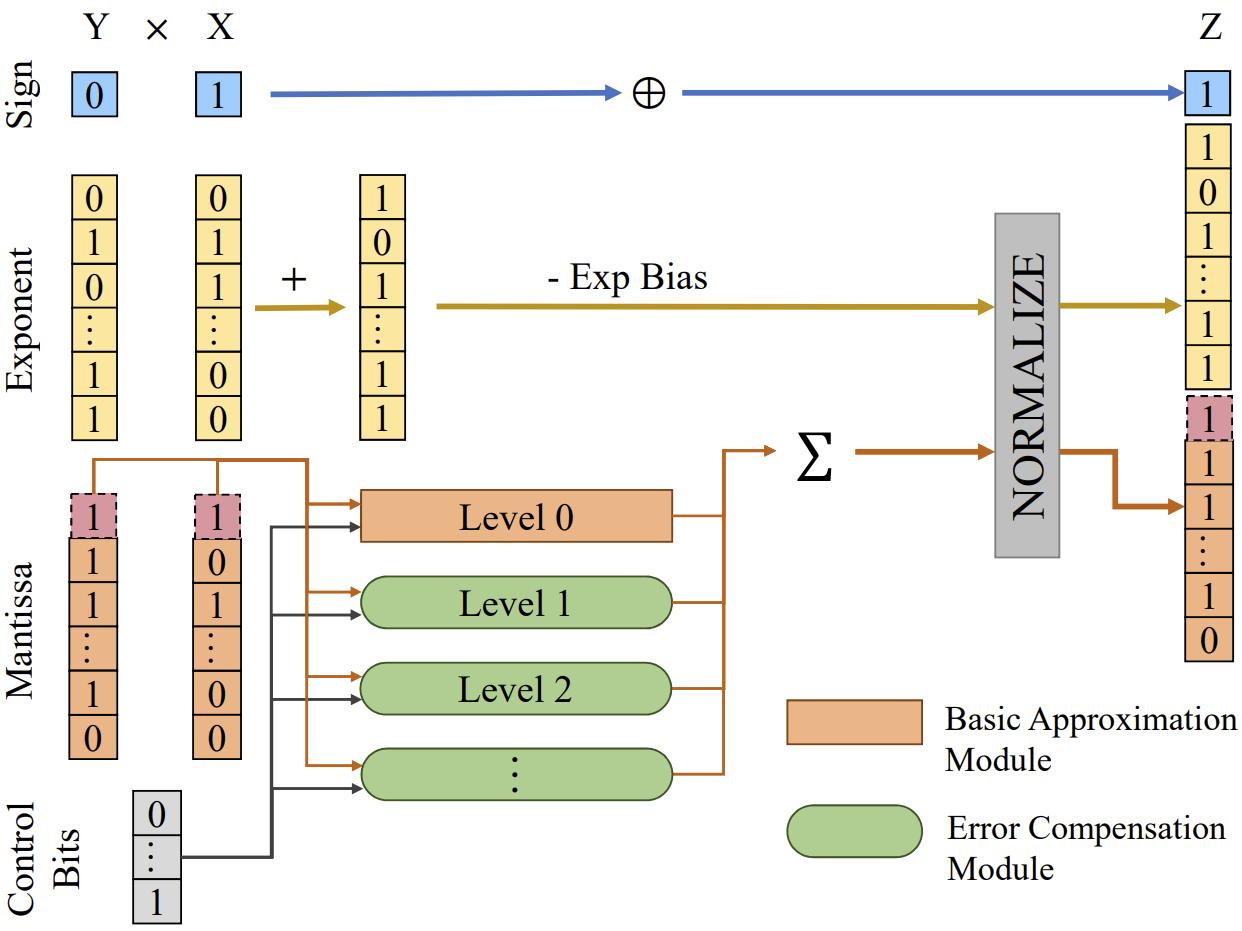
\includegraphics[width=\linewidth]{figs/AC-AM-OU_arch.png}
    \end{minipage}
    }
    \subfigure[不同划分等级下的误差分布图]{
    \label{AC:AM:Fig:OU_error}
    \begin{minipage}[t]{0.43\linewidth}
    \centering
    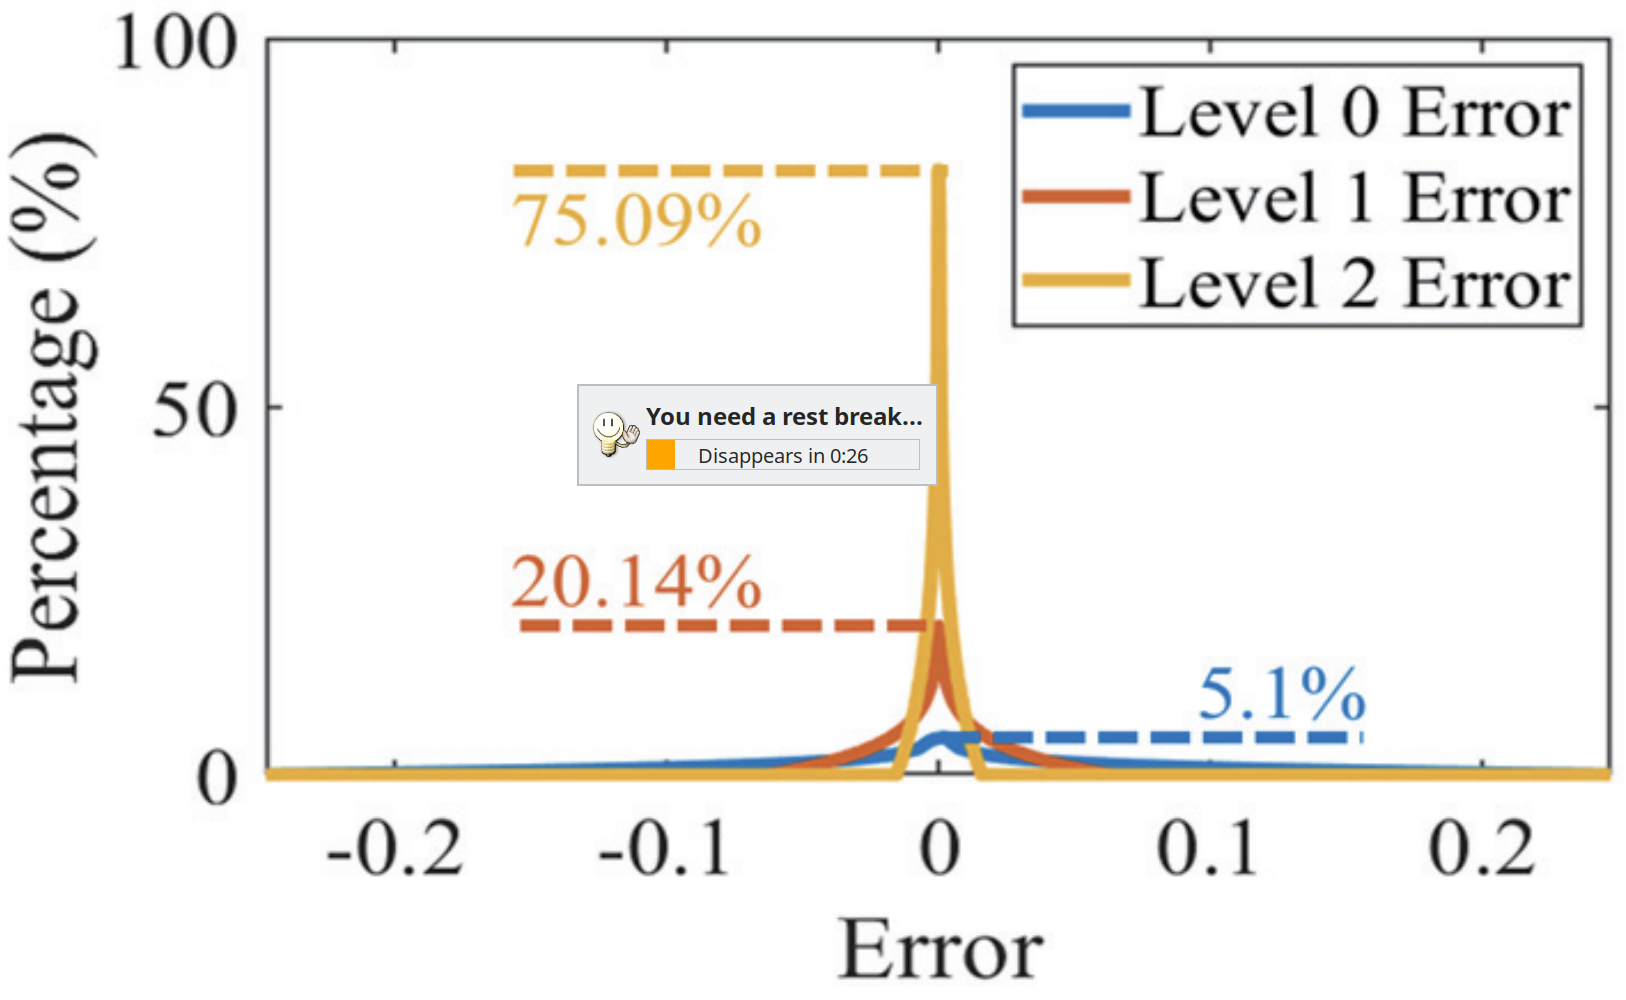
\includegraphics[width=\linewidth]{figs/AC-AM-OU_error.png}
    \end{minipage}
    }
\caption{论文所提出的近似浮点数乘法器架构图和不同划分等级下的误差分布}
\label{AC:AM:OU}
\end{figure}
图\ref{AC:AM:OU}展示了论文提出的近似浮点数乘法器的整体结构图和不同划分等级下的误差分布,可以看到随着划分次数的增加,误差在指数级减小。
尽管该方法是针对浮点数乘法器提出的,但经过简单的修改也可用于定点数乘法器。

(3)自动化方法(Automated method)

将设计近似乘法器的问题建模成搜索问题,能够利用计算机在短时间内生成大量具有不同精度和不同性能的近似乘法器。在自动化方法中,由捷克布尔诺理工大学(Brno University of Technology)可进化硬件(Evolvable HardWare, EHW)研究小组开发的、基于笛卡尔遗传规划(Cartesian Genetic Programming, CGP)\cite{CGP_2008,CGP_2011}的遗传算法(Genetic algorithm)取得了相当出色的效果。2016年,EHW的研究人员利用CGP设计了面向人工神经网络的近似乘法器\cite{AC:AM:CGP_2016},以精度下降小于2.80\%的代价节省了91\%的功耗。

CGP起源于Miller等人于1997年开发的一种进化数字电路的表示方法\cite{CGP_1997},在1999年第一次出现\cite{CGP_1999},其通用形式于2000年被正式提出\cite{CGP_2000}。
在CGP中,一个电路由一张有向无环图(Directed Acyclic Graph, DAG)进行表示,每个节点由一串整数组成,分别代表该节点从哪个节点获得数据以及节点对数据执行什么操作,输出没有被使用的节点可以被忽略。将所有的整数按照顺序排列,并在最后加上表示电路输出的节点编号便是电路对应的CGP形式。
\begin{figure}[!htb]
    \centering
    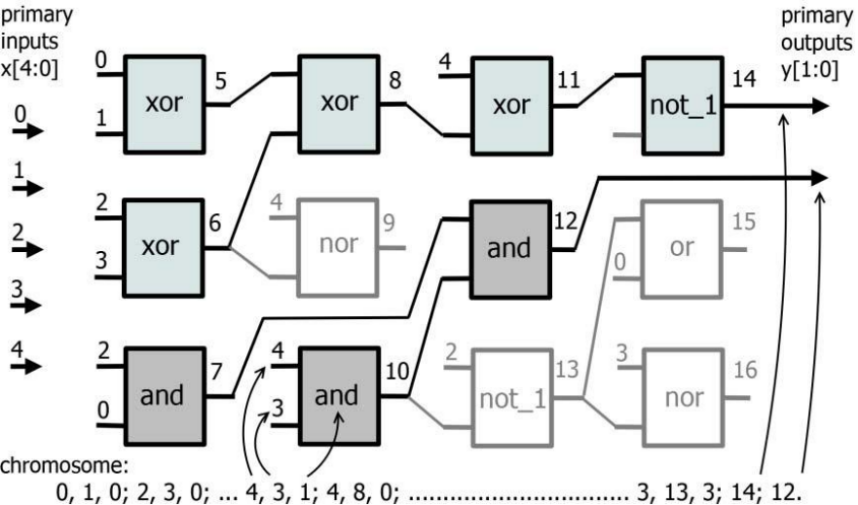
\includegraphics[width=0.8\linewidth]{figs/AC-AM-CGP.png}
    \caption{一个具有5比特输入、2比特输出的组合逻辑门级网表及其对应的CGP表示}
\label{AC:AM:CGP}
\end{figure}
图\ref{AC:AM:CGP}展示了一个具有5比特输入、2比特输出的组合逻辑门级网表及其对应的CGP表示,可以看到有4个门没有被使用。容易想到,若将一个精确乘法器的电路结构转换为CGP形式,那么改变CGP的表示形式便相当于改变了电路的功能,得到了近似乘法器。
Mrazek等人首先把8比特精确乘法器的不同电路实现结构转换成了CGP格式,然后随机改变CGP中的一部分整数得到近似乘法器,挑选出精度、延迟和功耗都较优的电路作为新的基础电路,不断迭代,在有限的时间内得到了均匀分布下误差较小、性能较高的471个近似乘法器,和430个近似加法器一起组成了一个开源的近似算术单元库EvoApprox8b\cite{AC:AM:CGP_Evoapprox8b}。考虑到许多应用中乘法器的输入数据分布并不是均匀的,在修改遗传算法中的目标函数后,CGP也可以被用于生成面向特定分布的高质量近似乘法器\cite{AC:AM:CGP_2019}。
如果乘法器的位宽较大,CGP等自动化方法生成的近似乘法器往往无法快速得到误差的边界,文献\cite{AC:AM:CGP_32bit}将近似等价性检查的形式化技术集成到CGP的搜索中,能够将搜索推向可快速验证的近似电路,方法通过ABC\cite{LS:ABC}工具实现,并对最大32比特位宽的乘法器进行了评估,结果显示提出的方法在几小时内生成了一组高质量的32位近似乘法器。

(4)近似电路综合(Approximate circuit synthesis)

近似电路综合(Approximate Circuit Synthesis)\cite{AC:ALS:survey}是近似逻辑综合的一个细分方向,着重于近似算术单元的生成,属于近似电路设计方法中功能近似(见\ref{approximate_computing_advance}有关功能近似的定义)的一种。
给定一个精确电路的描述和约束(通常是误差),近似电路综合不需要知道具体的电路功能,自动化生成满足精度的电路实现,与自动化方法相比,近似电路综合可直接应用于各种算术单元,通用性更强。近似电路综合可以通过网表转换(Netlist transformation)或布尔重写(Boolean rewriting)的方式实现,
\begin{figure}[!htb]
    \centering
    \subfigure[网表转换方法实现近似电路,左:精确电路的门级网表,右:生成的近似电路的门级网表]{
    \label{AC:ALS:survey_net_trans}
    \begin{minipage}[t]{\linewidth}
    \centering
    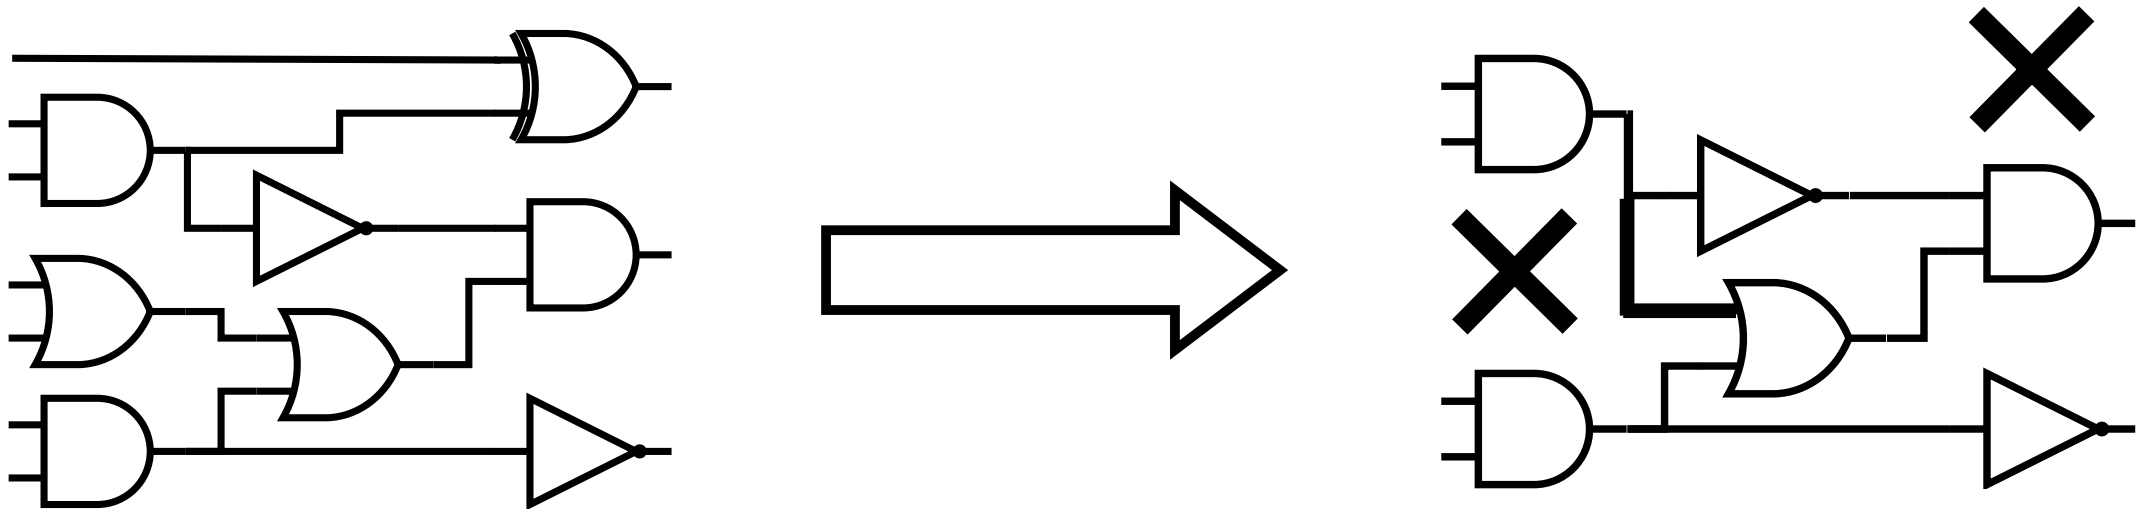
\includegraphics[width=0.8\linewidth]{figs/AC-ALS-survey_net_trans.png}
    \end{minipage}
    }
    \subfigure[布尔重写方法实现近似电路,左:精确电路的真值表,右:生成的近似电路的真值表]{
    \label{AC:ALS:survey_bool_rewr}
    \begin{minipage}[t]{\linewidth}
    \centering
    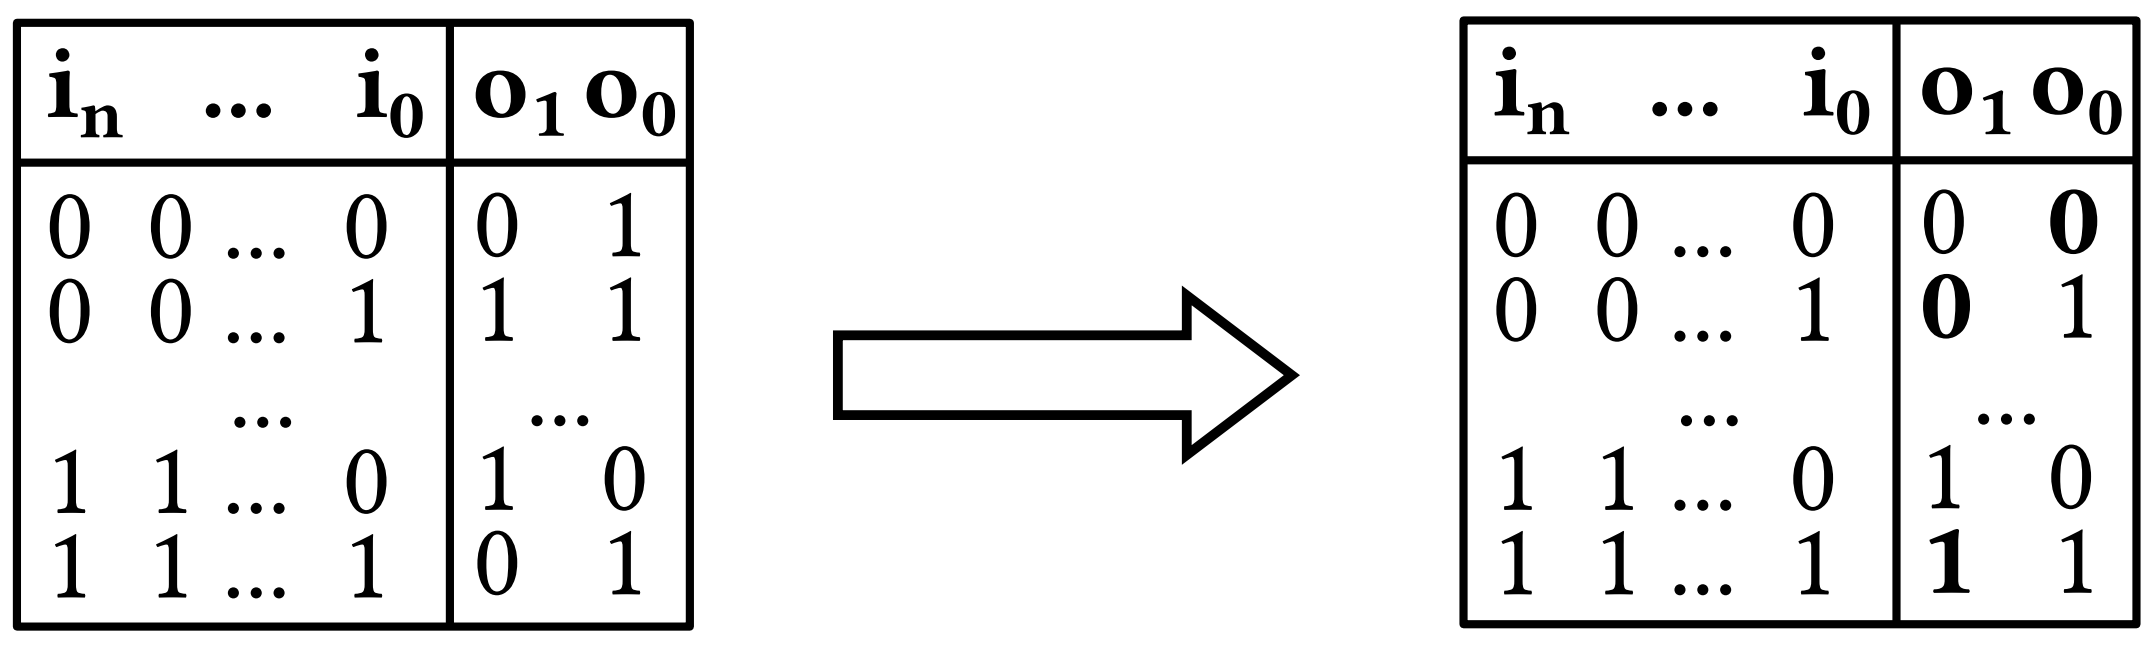
\includegraphics[width=0.75\linewidth]{figs/AC-ALS-survey_bool_rewr.png}
    \end{minipage}
    }
\caption{实现近似电路综合的两种常见方式}
\label{AC:ALS:survey_ACS_two_methods}
\end{figure}
图\ref{AC:ALS:survey_ACS_two_methods}举例展示了两种实现方式的区别,具体来讲,网表转换方式通过移除一些逻辑节点或用导线直接替换节点来对精确电路的门级网表进行简化,以达到减小面积和降低功耗的目的,而布尔重写方式则着重于修改抽象级别更高的真值表,使对应的布尔表达式更简洁紧凑。

文献\cite{AC:ALS:ALSRAC}采用网表转换的方法,利用重替换(resubstitution)算法\cite{LS:resub}不断尝试修改电路的局部结构,每次修改后用仿真的方式确定误差,直到找到满足精度要求的电路后退出。该方法被Meng等人基于ABC\cite{LS:ABC}实现并命名为ALSRAC,实验结果表明,ALSRAC产生的近似电路的面积与国际前沿工作相比减小了7\%-18\%。


\subsection{基于查找表编码的FPGA近似乘法器}

在介绍有关FPGA近似乘法器的工作之前,对FPGA的结构及乘法实现原理做一个介绍是必要的。
在FPGA中,算术操作通常由DSP模块实现,但DSP电路的面积只占整个FPGA芯片的5\%,且位置固定\cite{FPGA:DSP},这意味着某些需要大量乘法的应用比如DNN无法在FPGA上被有效的映射\cite{FPGA:Math}。相对应的,FPGA中存在着丰富的查找表单元,能够和布线资源一起实现复杂的函数功能,某些充分考虑LUT特性的设计能够在FPGA上实现相当高的性能\cite{FPGA:PolyLUT}。
然而,一块FPGA芯片的容量是有限的,对于大型设计来讲往往需要将其划分后部署到不同的FPGA芯片上,这会极大地降低电路的性能。同时FPGA中的布线资源昂贵,如果查找表单元使用的过多,有可能会造成布线拥塞,也会对电路的性能造成影响。
所以有必要在FPGA中使用近似乘法器来提高乘法的效率,降低FPGA资源的使用量,提高电路的性能。

\begin{figure}[!h]
    \centering
    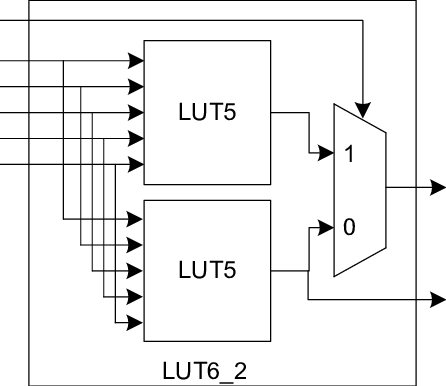
\includegraphics[width=0.5\linewidth]{figs/FPGA-LUT6_2.png}
    \caption{一个典型的拥有6个输入的LUT结构图}
    \label{FPGA:Fig:LUT6_2}
\end{figure}

LUT通常由多路选择器MUX和SRAM构成,其大小可根据输入个数的不同进行区分,一个$n$输入的LUT包含$2^n -1$个MUX和$2^n$个SRAM,能实现任意的$n$输入函数(共$2^{2^n}$个),可看作两个$n-1$的输入LUT和一个二选一MUX的组合。
目前最常用的LUT的输入个数为6\cite{FPGA:VIB},简称为LUT6。图\ref{FPGA:Fig:LUT6_2}展示了一个由两个LUT5组成的LUT6示意图,被称为LUT6\_2。LUT6\_2共包含$64$个SRAM,在编码后每个SRAM都有一个确定的值,被称为初始(Initial, INIT)值,不同INIT值的组合能够实现不同的函数,一共有$2^{64}$种组合,能够实现任意的6输入函数。

\begin{figure}[!h]
    \centering
    
\includegraphics[width=0.4\linewidth]{figs/FPGA-carry_chain.png}
    \caption{一种2比特位宽的FPGA进位链结构示意图}
    \label{FPGA:Fig:carry_chain}
\end{figure}

虽然LUT能够实现特定输入数下的任意单输出函数,但对多输入多输出的算术操作的运算效率并不高。
考虑到加法使用最频繁,为了提高性能,FPGA引入了进位链来降低加法的进位延迟,
一种典型的2比特位宽的进位链结构如图\ref{FPGA:Fig:carry_chain}所示,由两个进位单元级联而成,每个进位单元包含一个LUT和一个伪全加器FA$'$,每个LUT的结构如图\ref{FPGA:Fig:LUT6_2}中的LUT6\_2所示。
根据式\eqref{EM:Eq:CLA}得全加器的进位信号:$c_{i+1} = p_i c_i  + \overline{p_i} g_i$,求和信号:$s_{i} = p_i \oplus g_i$,则可利用LUT6\_2中的两个LUT5产生进位的传播信号和生成信号送给伪全加器FA$'$,伪全加器FA$'$通过一个异或门XOR和一个二选一MUX进行求和及进位输出,MUX可由延迟较低的传输管结构实现。通过级联更多的进位单元可实现更大位宽的进位链。

文献\cite{AC:AM:FPGA:SMApproxLib}通过手动修改精确乘法器中用于部分积累加的LUT的INIT值,设计了几个拥有不同误差和不同硬件成本的近似乘法器,提出并开源了第一个面向FPGA领域的近似乘法器库SMApproxLib。类似地,文献\cite{AC:AM:FPGA:CaCc,AC:AM:FPGA:FPT22,AC:AM:FPGA:TCAD22}也采用了修改精确模式下LUT中SRAM编码的方法来得到误差不同的近似乘法器。



\section{逻辑综合介绍}


\subsection{Yosys和ABC}

\begin{figure}[!htbp]
    \centering
    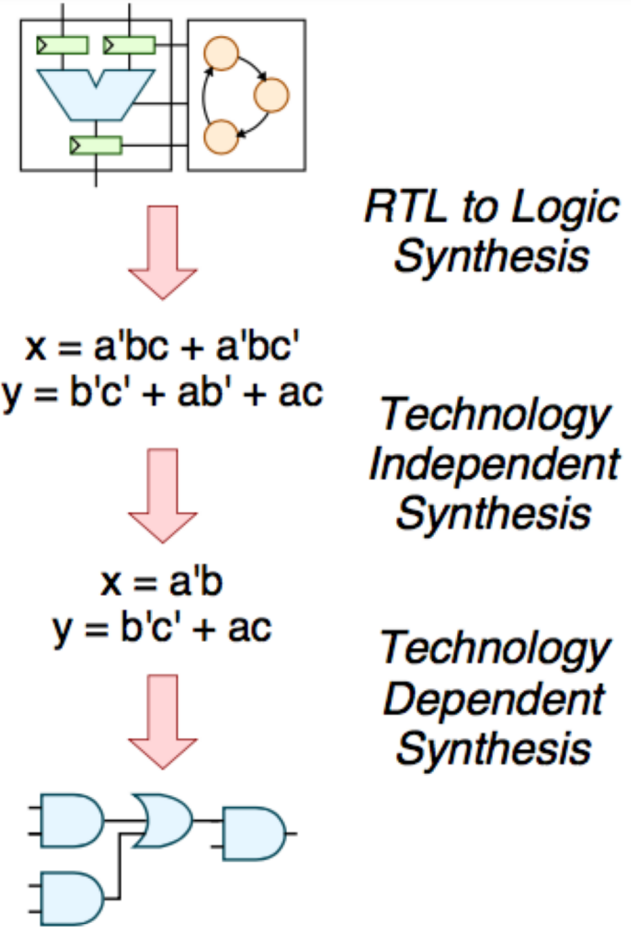
\includegraphics[width=0.4\linewidth]{./figs/LS-flow.png}
    \caption{传统逻辑综合流程图}
    \label{LS:flow}
\end{figure}

\begin{figure}[!htbp]
    \centering
    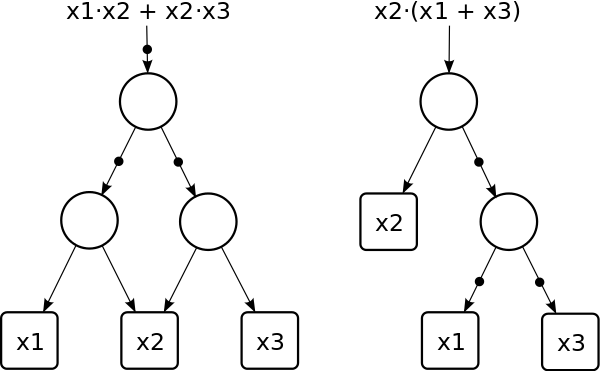
\includegraphics[width=0.6\linewidth]{./figs/LS-two_AIG.png}
    \caption{函数$x_2 (x_1 + x_3)$的两种不同的AIG实现}
    \label{LS:two_AIG}
\end{figure}


图\ref{LS:flow}展示了传统逻辑综合的流程图,首先将用户设计的寄存器传输级电路读入并解析,然后进行一系列工艺无关的逻辑优化操作,最后进行工艺相关的映射,生成门级网表。在现代EDA工具中,解析后电路中的组合逻辑部分通常由一个有向无环图进行表示,被称为布尔网络\cite{FPGA:CLB_Anderson},网络中的节点代表逻辑函数,边代表连接关系,逻辑综合进行的一系列优化及映射操作都基于该网络实现。
在一个布尔网络中\cite{LS:exact_rewriting,FPGA:Jason_Cong_1993,LS:Verification_after_synthesis},一个节点的扇入(Fanin)和扇出(Fanout)分别指该节点的输入节点和输出节点;
假设存在一条路径从节点$v$到节点$w$,则$v$是$w$的传递扇入(Transitive fanin),$w$是$v$的传递扇出(Transitive fanout);
网络的主要输入(Primary Inputs, PIs)是指所有的无扇入节点,网络的主要输出(Primary Outputs, POs)是指所有与外部相连的节点;
一条路径的长度指经过的节点数目;
节点的深度或级数指从网络的所有主要输入到该节点的所有路径中最长路径的长度;
最大节点深度被称为网络的深度。

% 图\ref{LS:boolean_net}展示了一个简单的布尔网络的示意图,可以看作是有5个输入、6个输出、7个节点、16条边的DAG,

% \begin{figure}[!htbp]
%     \centering
%     \includegraphics[width=0.8\linewidth]{./figs/LS-boolean_net.png}
%     \caption{一个简单的布尔网络示意图}
%     \label{LS:boolean_net}
% \end{figure}

AIG(And-Inverter Graph)是目前一种被广泛用来对逻辑函数进行表示和优化的有向无环图\cite{LS:AIG},在AIG中,节点分为主要输入节点、主要输出节点和2输入的与门节点三种类型,边包括取反和不取反两种情况,主要输入节点没有输入边,主要输出节点可能有输出边。一个逻辑函数可由不同结构的AIG表示,图\ref{LS:two_AIG}展示了函数$x_2 (x_1 + x_3)$两种不同的AIG实现。基于AIG,由Berkeley大学研发的的逻辑综合与验证工具ABC\cite{LS:ABC}在学术界和工业界获得了广泛的关注和赞誉。ABC可以对AIG进行逻辑优化和工艺映射,逻辑优化的目标是最小化AIG的规模和深度,映射目标是最小化LUT或ASIC电路的面积和延迟。


% 研究表明\cite{LS:structural_bias},AIG的映射结果会受到结构偏差(Structural bias)问题的影响,具体来说,同一个AIG进行不同的变换后会有不同的映射结果,且质量差别较大,这是由于AIG结构的不同导致映射器无法发现更优的解。图\ref{LS:structural_bias}展示了结构偏差问题的存在对LUT映射质量产生影响的一个示例,

% \begin{figure}[!htbp]
%     \centering
%     \includegraphics[width=\linewidth]{./figs/LS-structural_bias.png}
%     \caption{结构偏差问题影响LUT映射质量的一个示例}
%     \label{LS:structural_bias}
% \end{figure}


在逻辑优化阶段,ABC存在着许多不同的命令对AIG进行变换和化简,典型的命令包括balance, refactor, rewrite等,不同的优化命令会对AIG产生不同的优化效果,开发人员根据经验预先设定了一些优化脚本(如resyn2)对不同的电路进行使用。然而,不同命令的组合及顺序对逻辑优化的效果有很大影响,并且当优化进行到一定程度后,继续优化并不一定会对后续的映射操作起到正面效果\cite{LS:PIMap},因此必须针对不同的电路提供不同的优化序列,以达到对不同电路都能实现良好提升的目的。为给定的布尔逻辑网络寻找较优逻辑优化命令组合的问题被称为序列探索。

ABC能够利用AIG对布尔网络进行有效地表示和变换,但在电路解析方面能力不足。目前使用最广泛的硬件描述语言(Hardware description language)是Verilog-2005,被大多数EDA工具支持。Yosys\cite{LS:yosys}是一款开源的Verilog解析工具,支持绝大部分Verilog-2005语法,与ABC结合能够完成从Verilog到门级网表的全流程工作。

\subsection{用来表示布尔网络的不同DAG形式}

(1)XAIG

\begin{figure}[!htbp]
    \centering
    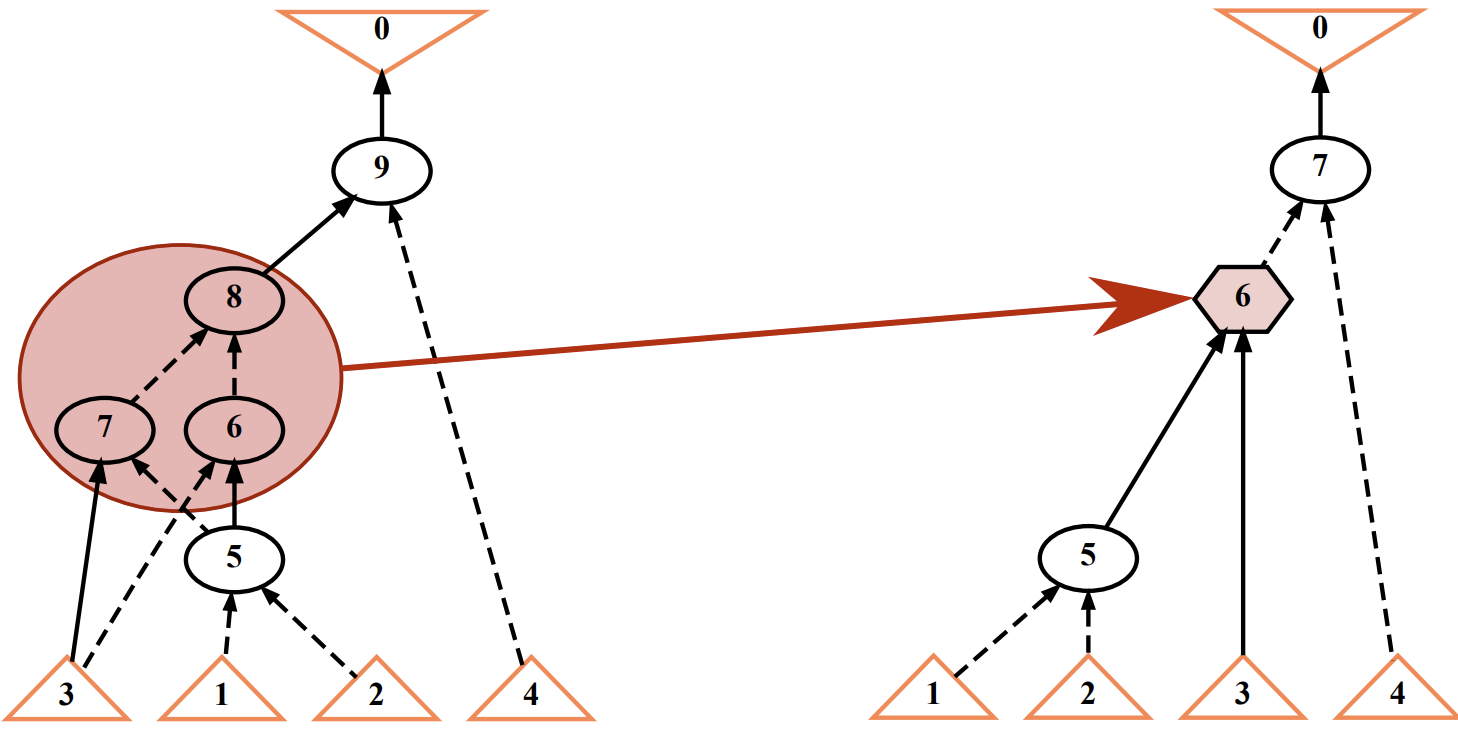
\includegraphics[width=0.75\linewidth]{./figs/LS-XAIG.png}
    \caption{函数$ \overline{ \overline{x_1 + x_2} \oplus x_3} \cdot \overline{x_4} $的AIG和XAIG,圆圈代表AND节点,六边形代表XOR节点,虚线边代表取反操作}
    \label{LS:XAIG}
\end{figure}

在AIG中,一个2输入异或门至少需要3个节点才能表示,这导致AIG无法对异或密集型电路进行高效地表示和优化,因此有工作提出了XAIG(Xor-And-Inverter Graph),在AIG中引入2输入的XOR节点,提高异或操作的表达效率\cite{LS:XAIG_Microelec_Relia,LS:XAIG_ddecs,LS:XAIG_iwls}。
图\ref{LS:XAIG}展示了函数$ \overline{ \overline{x_1 + x_2} \oplus x_3} \cdot \overline{x_4} $的AIG和XAIG,其中圆圈代表AND节点,六边形代表XOR节点,虚线边代表取反操作,可以看到XOR节点的引入能够降低图的规模。XAIG也被称为XAG(Xor-And Graph)。

(2)MIG

与XAIG的提出类似,有工作发现AIG能对控制电路进行高效地表达和变换,但对算术电路的操作效率较低,于是提出了适用于算术电路的MIG(Majority-Inverter Graph)\cite{LS:MIG}形式。在MIG中,除了输入节点外,每个节点表示一个3输入的Majority门,用符号$\langle \rangle$表示,定义为:
\begin{equation}
    \label{LS:MIG:Eq:Majority}
    \langle xyz \rangle = xy + xz + yz = (x + y) (x + z) (y + z)
\end{equation}

(3)XMG

对MIG引入3输入的XOR节点,能够提高某些函数的表达效率,对应的DAG实现被称为XMG(Xor-Majority Graph)\cite{LS:XMG_2017}。图\ref{LS:XMG}展示了函数$\langle x_1,x_2,(x_3 \oplus x_4) \rangle$分别在AIG、MIG和XMG中的表示,虚线代表取反操作,可以看到XMG使用的节点数目最少\cite{LS:XMG_2024}。

\begin{figure}[!htbp]
    \centering
    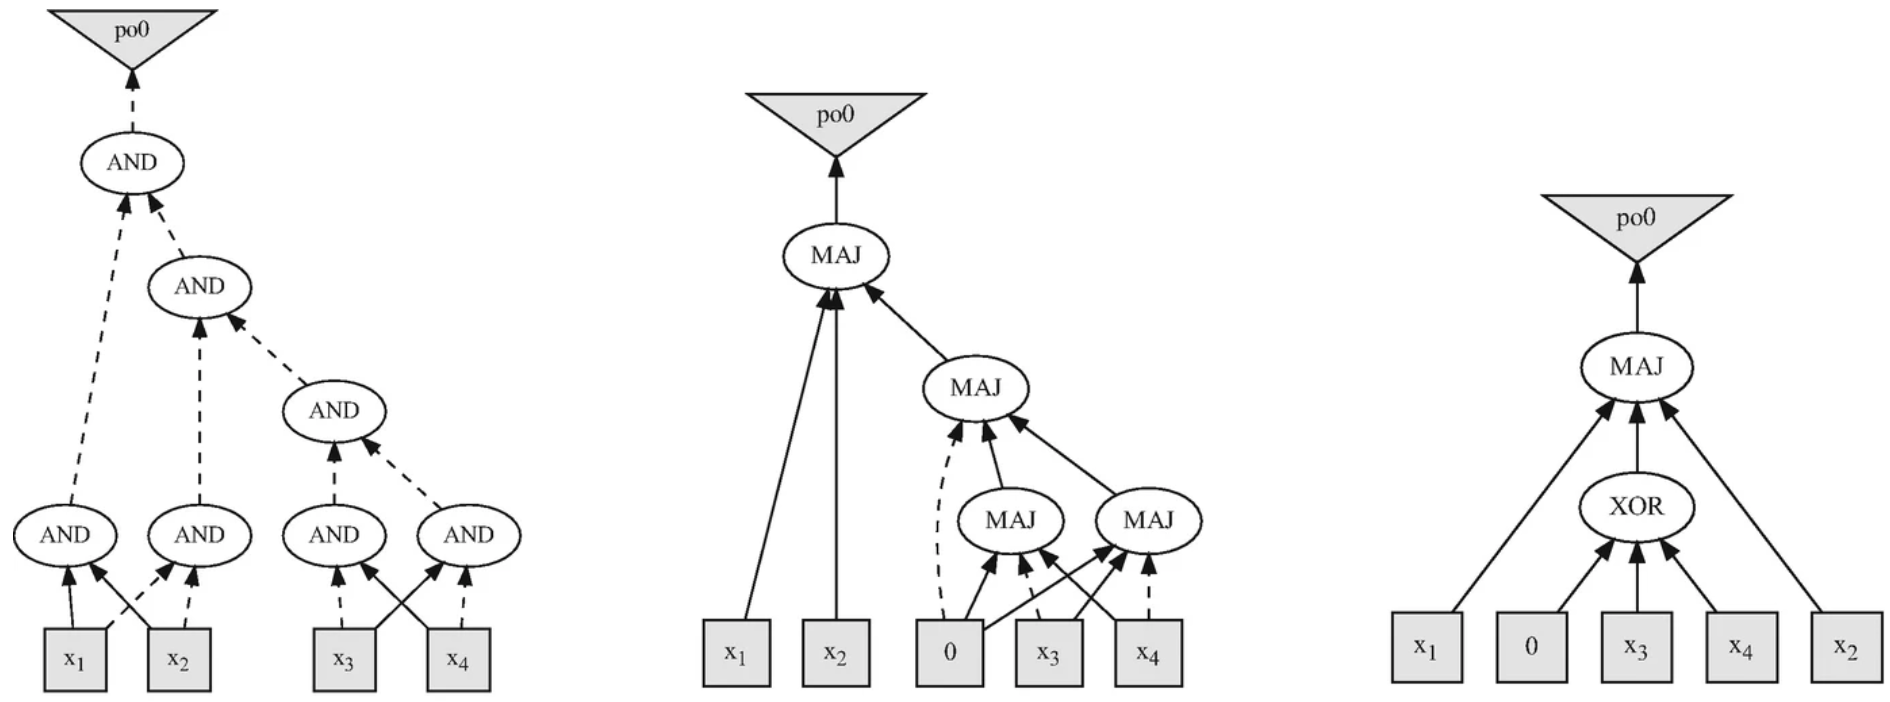
\includegraphics[width=\linewidth]{./figs/LS-XMG.png}
    \caption{函数$\langle x_1,x_2,(x_3 \oplus x_4) \rangle$分别在不同DAG中的表示,从左到右依次为:AIG、MIG、XMG,虚线代表取反操作}
    \label{LS:XMG}
\end{figure}

\subsection{MFFC} \label{MFFC}

在一个布尔网络中,节点$v$的一个锥(Cone)$C_v$是指$v$和$v$的传递扇入节点的集合(不包括网络的主要输入),锥中任意节点到$v$的路径都在锥内,$v$被称为锥的根节点,易知$v$可以有多个锥\cite{LS:exact_rewriting,FPGA:Jason_Cong_1993}。扇入节点数量小于等于$K$的锥被称为$K$可行锥($K$-feasible cone)\cite{FPGA:Jason_Cong_1999_cut_ranking}。

节点$v$在锥$C_v$下的一个割(Cut)是$C_v$的一个划分$(X,\overline{X})$,其中$\overline{X}$是$v$的一个锥。当$\overline{X}$是一个$K$可行锥时,割$(X,\overline{X})$被称为$K$可行割($K$-feasible cut)\cite{FPGA:Jason_Cong_1999_cut_ranking}。$\overline{X}$的扇入节点集合$L$满足以下两个性质:
\begin{itemize}
    \item 任意一条从网络的主要输入到节点$v$的路径至少会经过$L$中的一个元素;
    \item 对于$L$中的任何一个节点$l$,至少存在一条从主要输入到$v$的路径经过$l$且不经过$L$中的其他节点。
\end{itemize}
图\ref{LS:z_cone_two_cuts}展示了节点z的一个锥\{z,x,a,d,c,b,e\}和两个割\cite{FPGA:CLB_Anderson}cut1、cut2,易知cut1和cut2均是3可行割。
\begin{figure}[!htbp]
    \centering
    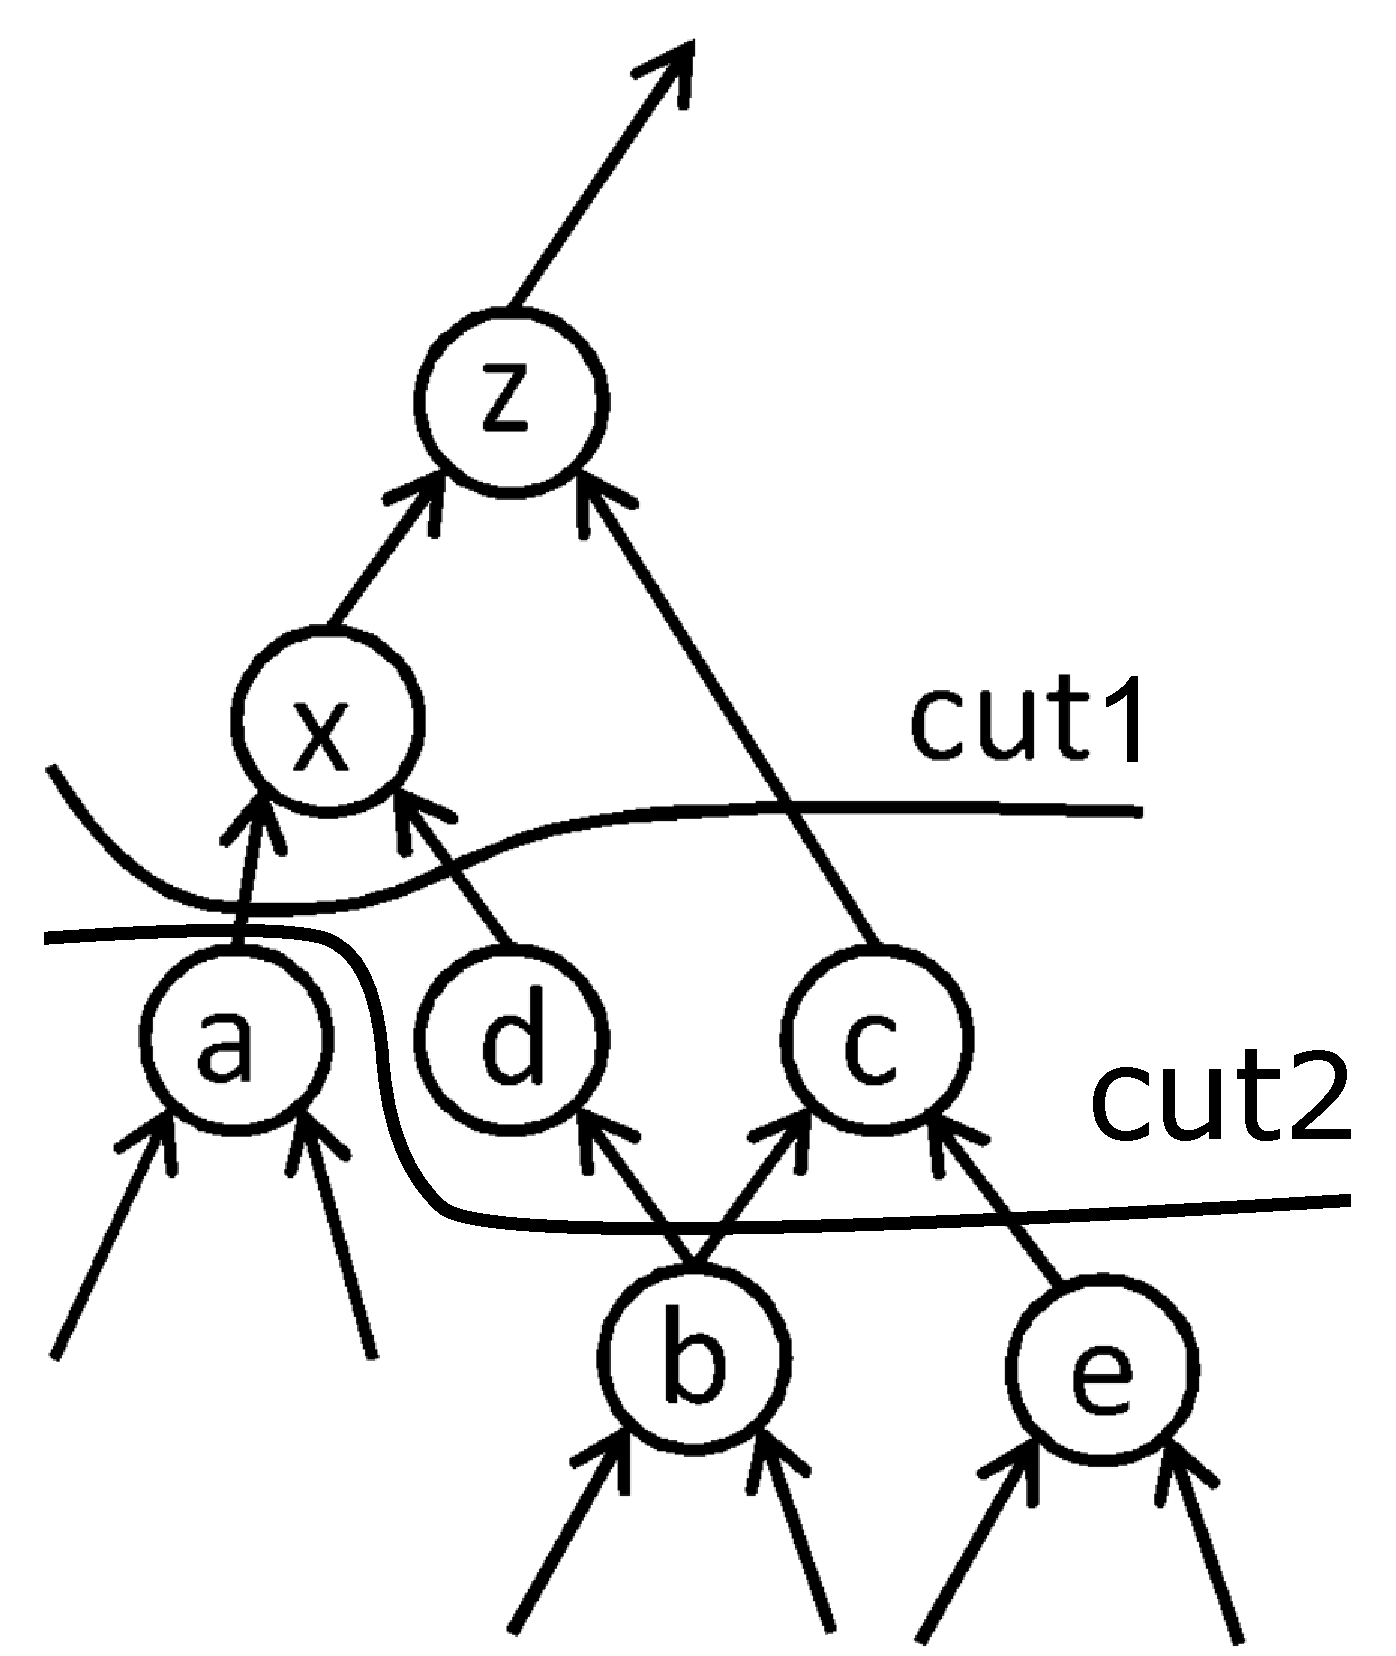
\includegraphics[width=0.4\linewidth]{./figs/LS-z_cone_two_cuts.pdf}
    \caption{节点z的一个锥\{z,x,a,d,c,b,e\}和两个割cut1与cut2}
    \label{LS:z_cone_two_cuts}
\end{figure}

若锥$C_v$内任意节点的扇出均在锥内,则称$C_v$为节点$v$的无扇出锥(Fanout Free Cone, FFC)。$v$的无扇出锥可以有多个,存在一个最大的无扇出锥,被称为$v$的最大无扇出锥(Maximum Fanout Free Cone, MFFC),记为MFFC$_v$。易知MFFC有以下性质\cite{LS:exact_rewriting,FPGA:Jason_Cong_1993,FPGA:Jason_Cong_patition}:
\begin{itemize}
    \item 一个节点的MFFC有且只有一个;
    \item 若 $w \in \text{MFFC}_v$,则$\text{MFFC}_w \subseteq \text{MFFC}_v$;
    \item 两个MFFC要么不相交,要么一个包含另一个;
    \item $\text{MFFC}_v$中节点的值只会影响到$v$和$v$的传递扇出。
\end{itemize}
\begin{figure}[!htbp]
    \centering
    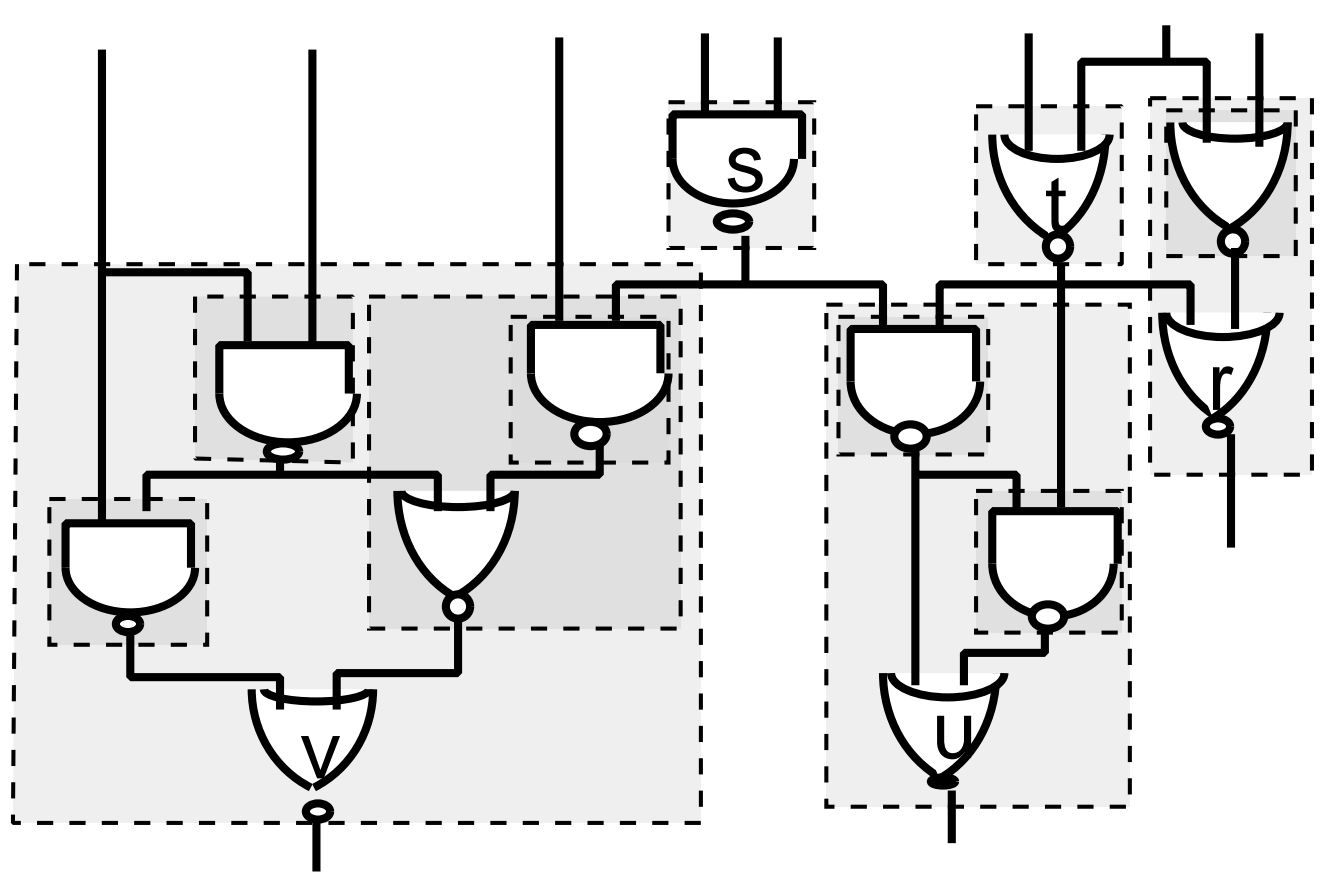
\includegraphics[width=0.5\linewidth]{./figs/LS-MFFC.png}
    \caption{不同节点的最大无扇出锥}
    \label{LS:MFFC}
\end{figure}
图\ref{LS:MFFC}展示了一个布尔网络中不同节点的MFFC,以不同灰度的阴影区域表示,可以看到各MFFC满足上述性质。


\subsection{电路划分}

当布尔网络的规模太大时,单个优化命令的运行时间变长,序列探索时单次迭代花费的时间显著增加,导致无法在一个可接受的时间范围内得到一个较优的命令组合,通过划分将大型网络分割成较小的子网络来并行地探索,能够大大减少运行时间。

(1)超图划分

一个网络的DAG图既可以转换成普通图(一条边只连接两个顶点),也可以转换成超图(一条边可以连接超过两个顶点),考虑到电路中的输出往往都是多扇出的,超图能够更好地体现其连接性,因此将电路转换成超图进行划分是一个较好的选择\cite{LS:LSOracle}。

\begin{figure}[!htbp]
    \centering
    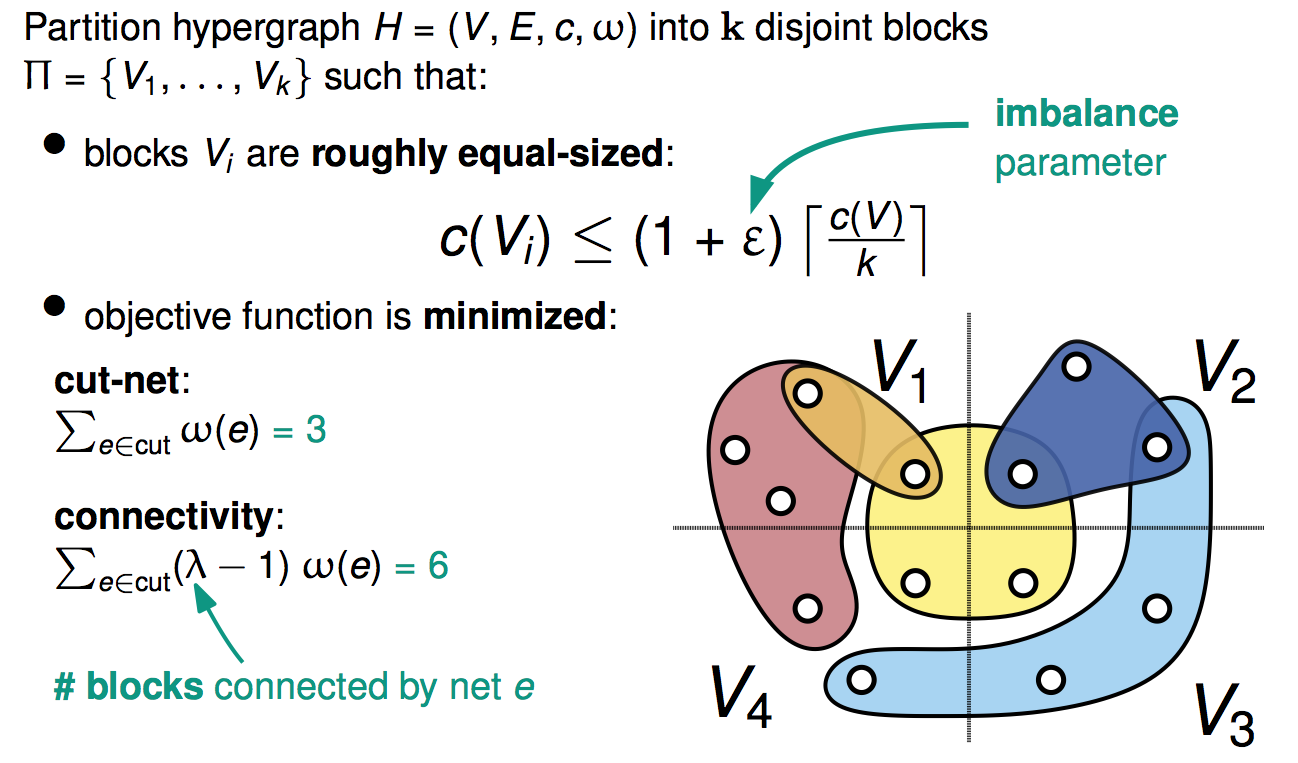
\includegraphics[width=0.8\linewidth]{./figs/Hypergraph_partition.png}
    \caption{超图划分问题的定义}
    \label{Hypergraph_partition}
\end{figure}

超图划分(Hypergrap partitioning)\cite{KaHyPar}能够对节点进行分类,将所有的节点划分为$k$个大致相等的部分,同时最小化基于边定义的目标函数,常见的目标函数有割边重要性和子图连通性,其中割边重要性是指被切割的超边的权重之和,而子图连通性则会同时考虑割边权重和割边连接的子图的数量。图\ref{Hypergraph_partition}展示了超图划分问题的定义以及两种目标函数的形式。
目前最常用的超图划分算法是多层(Multilevel)方法,由三个步骤组成:(1)粗化:对超图中不同连接紧密程度的点进行逐级合并以降低超图的规模;(2)初始划分:粗化完成后得到一个小的超图并对其进行初始划分;(3)细化:逐级分解原先合并的点并执行划分操作,每一次划分后利用局部搜索的方法来调整位于边界上的点以最小化目标函数,直到划分后子图的数目满足要求。

(2)自然划分

通常来讲,EDA工具对电路进行解析后生成布尔网络时会把寄存器与组合逻辑分开,将寄存器的输入变成组合逻辑的输出,将寄存器的输出变成组合逻辑的输入。有工作发现,良好设计的电路中流水线(Pipeline)技术充分,能够将整个电路“自然”地切分成数个均匀的组合逻辑块,转换成布尔网络后对应多个相互独立的DAG。基于此发现,文献\cite{Moucheng_Yang}提出了一种“自然划分(Natural partitioning)”的布尔网络分割方法,该方法基于ABC\cite{LS:ABC}实现,能够对一个大型AIG进行分簇,簇与簇之间没有连接,然后对所有的AIG簇并行地进行LUT映射以提高速度,对13个大型电路的测试结果表明,映射速度平均提高了5.76倍,面积略微增加了0.57\%,延迟保持不变。

(3)基于MFFC和带约束超图划分的有向无环划分

普通的超图划分并没有考虑DAG有向无环的特点,文献\cite{FPGA:Jason_Cong_patition}首先对一个网络进行遍历,利用MFFC缩小超图的规模,之后基于带约束的多层划分方法,提出了一个面向FPGA领域的有向无环划分方案,与普通超图划分相比割边数量更少、分割质量更高。

\subsection{强化学习}

强化学习是机器学习中的一个领域,强调一个智能体(Agent)如何基于环境(Environment)行动,以取得最大化的预期利益,是除了监督学习和非监督学习之外的第三种基本的机器学习方法。强化学习通过感知所处环境的状态(State)对动作(Action)的 反应(Reward),来指导更好的动作,从而获取最大的收益(Return)。以游戏为例,如果在游戏中采取某种策略可以取得较高的得分,那么就进一步“强化”这种策略,以期继续取得较好的结果。目前,强化学习在某些领域已经被证明了达到人类水平,甚至优于人类,比如早在2016年由谷歌研发的电脑围棋软件AlphaGo\cite{AI:AlphaGo}就已经击败了韩国围棋冠军李世石。

强化学习基于马尔科夫决策过程(Markov decision process),即当前状态包含了对未来预测所需要的所有信息,过去信息对未来预测不重要,关注点在于“探索未知领域”和“利用已有知识”的平衡,其实现算法分为有模型学习(Model-Based)和免模型学习(Model-Free)两类,其中免模型学习更容易实现,迁移性也更好,得到了广泛的研究。

\subsection{序列探索}

学术界提出了多种方法用来对逻辑综合中不同命令的组合及顺序进行探索,包括基于强化学习的方法、利用贝叶斯优化进行搜索、以及基于图神经网络进行预测等,下面分别进行介绍。

(1)基于强化学习的方法

\begin{figure}[!htbp]
    \centering
    \includegraphics[width=0.7\linewidth]{./figs/LS-DRiLLS-framework.png}
    \caption{基于强化学习的序列优化方法DRiLLS的架构图}
    \label{LS:DRiLLS:Fig:framework}
\end{figure}

假设$\mathbb{A} = \{ a_1,\ a_2,\ a_3,\ \cdots,\ a_n \}$代表$n$个相互之间没有依赖的优化命令集合,$k$表示优化序列长度,则可能的命令组合情况一共有$n^k$种。
文献\cite{LS:DRiLLS}提出了一种基于强化学习的序列优化方法DRiLLS,DRiLLS利用A2C(Advantage Actor Critic)代理来探索序列空间。图\ref{LS:DRiLLS:Fig:framework}给出了DRiLLS的架构图,其中逻辑综合环境由Yosys和ABC实现,强化学习环境由A2C代理,与综合环境进行交互学习。DRiLLS将强化学习中的状态$state$定义为ABC中AIG的信息,包括主要输入输出数量、节点数、级数、寄存器数量、AIG中边的条数、以及AIG中反向边的数量。
同时,DRiLLS中强化学习的奖励函数是一个同时考虑面积和延迟的多目标函数,对于满足延迟约束且面积减少的优化序列,奖励最高(用+++表示),对于不满足延迟约束且面积增加的优化序列,奖励最低(用- - -表示),具体的奖励标准如表\ref{LS:DRiLLS:Table:reward}所示。

\begin{table*}[!htbp]
    \caption{DRiLLS中不同优化效果的序列对应的奖励情况}
    \centering
    \label{LS:DRiLLS:Table:reward}
    \includegraphics[width=0.7\linewidth]{./figs/LS-DRiLLS-reward_table.png}
\end{table*}

\begin{table*}[!htbp]
    \caption{实验结果}
    \centering
    \label{LS:DRiLLS:Table:results}
    \includegraphics[width=\linewidth]{./figs/LS-DRiLLS-results.png}
\end{table*}

表\ref{LS:DRiLLS:Table:results}展示了基于ABC\cite{LS:ABC}和EPFL测试集\cite{LS:EPFL_benchs_iwls,LS:EPFL_benchs_github}通过4种方法包括贪婪算法(Greedy algorithm)、手工设计的优化序列\cite{LS:DRiLLS:hand_craft}(Expert-crafted)、已有的最佳记录、DRiLLS在开源的7nm工艺库\cite{ASAP7_github}上得到的实验结果,其中DRiLLS的延迟约束是初始的未优化的电路直接映射得到的延迟。
可以看到,DRiLLS在不同的电路上均满足了延迟约束,面积平均提高了13.19\%,这显示了DRiLLS多目标奖励函数的有效性。


(2)利用贝叶斯优化搜索

逻辑优化中的序列探索问题可以归结为黑盒优化问题,文献\cite{LS:BOiLS}提出了BOiLS,利用贝叶斯优化对命令的组合及顺序进行探索。基于ABC,对于一个给定的AIG,BOiLS的目标是在$n$个优化命令中找到一个长度为$K$的序列对电路进行优化,序列的好坏通过ABC进行LUT映射后来评估,其质量由下面的公式进行表达:
\begin{equation}
    \label{LS:BOiLS:Eq:QoR}
    QoR = \frac{Area(seq)}{Area(ref)} + \frac{Delay(seq)}{Delay(ref)}
\end{equation}
其中$Area(ref)$和$Delay(ref)$分别代表对原始电路用resyn2进行优化和映射后LUT的个数和级数,$Area(seq)$和$Delay(seq)$分别代表BOiLS找到的优化序列对原始电路进行优化和映射后LUT的个数和级数。在BOiLS中,考虑的优化命令包括:rewrite, rewrite -z, refactor, refactor -z, resub, resub -z, balance, fraig, sopb, blut, dsdb,序列大小$K=20$。

\begin{figure}[!htbp]
    \centering
    \includegraphics[width=\linewidth]{./figs/LS-BOiLS-results.png}
    \caption{不同序列探索方法在迭代200次后的LUT映射结果}
    \label{LS:BOiLS:Fig:results}
\end{figure}

\begin{figure}[!htbp]
    \centering
    \includegraphics[width=\linewidth]{./figs/LS-BOiLS-results_2.png}
    \caption{不同方法在4个电路上的探索效率对比}
    \label{LS:BOiLS:Fig:results_2}
\end{figure}

基于EPFL电路集\cite{LS:EPFL_benchs_iwls,LS:EPFL_benchs_github},BOiLS与6个前沿工作进行了对比,包括:基于强化学习方法的DRiLLS\cite{LS:DRiLLS},标准贝叶斯优化(Standard Bayesian Optimization, SBO),遗传算法(Genetic Algorithm, GA),随机搜索(Random Search, RS),以及已有的最佳记录。每种方法限制的迭代次数为200,图\ref{LS:BOiLS:Fig:results}展示了不同方法的实验结果。可以看到,BOiLS在8/10个电路中都取得了最优结果,SBO在log2电路中效果最好,BOiLS紧随其后,显示了贝叶斯优化在逻辑综合序列探索中的巨大潜力。图\ref{LS:BOiLS:Fig:results_2}比较了不同优化方法在4个电路上的探索效率,结果显示,基于强化学习的序列搜索方法DRiLLS看起来似乎并没有比随机搜索强多少。

(3)基于图神经网络的方法

图卷积网络(Graph Convolutional Network, GCN)是一种用于处理图数据的深度学习模型,其目标是将传统的卷积神经网络和递归神经网络等深度学习方法扩展到图结构数据如社交网络、推荐系统、生物信息学等领域,填补深度学习对图数据处理方式的空缺。

\begin{figure}[!htbp]
    \centering
    \includegraphics[width=0.7\linewidth]{./figs/LS-Bulls-Eye-QoR_predictor.png}
    \caption{基于AIG和GCN的序列质量预测器}
    \label{LS:Bulls-Eye:Fig:QoR_predictor}
\end{figure}

\begin{figure}[!htbp]
    \centering
    \includegraphics[width=0.9\linewidth]{./figs/LS-Bulls-Eye-overall_framework.png}
    \caption{Bulls-Eye整体框架图}
    \label{LS:Bulls-Eye:Fig:overall_framework}
\end{figure}

文献\cite{LS:Bulls-Eye}首先利用GCN基于AIG提出了一个序列质量预测器,总体结构如图\ref{LS:Bulls-Eye:Fig:QoR_predictor}所示。预测器的输入包括AIG和优化命令序列(图中的Synthesis recipe),两者分别通过AIG嵌入网络和序列嵌入网络进行嵌入,拼接后经过四层全连接层进行输出。之后,在基于小型电路集上对预测器进行训练后,面对新的大型电路,通过主动学习(Active learning)的方式对预测器进行微调,以提高对新电路的预测准确率。最后,基于微调后的预测器,利用模拟退火算法对新电路生成一个高质量的优化序列,整体框架命名为Bulls-Eye,流程如图\ref{LS:Bulls-Eye:Fig:overall_framework}所示。Bulls-Eye的预测器在基于44个开源电路设计组成的数据集上进行训练,实验表明,训练后的模型在新的大型电路的序列质量预测任务中表现良好,微调后的模型准确率进一步上升。

\subsection{多种DAG联合优化}

基于MIG对算术电路的综合及映射效果比AIG更好这一特点,文献\cite{LS:LSOracle}提出了LSOracle,是第一个同时采用多种DAG形式对布尔逻辑电路进行表示和优化的开源异构逻辑综合框架。

\begin{figure}[!htbp]
    \centering
    \includegraphics[width=0.7\linewidth]{./figs/LS-LSOracle-flow.png}
    \caption{LSOracle流程图}
    \label{LS:LSOracle:Fig:flow}
\end{figure}

图\ref{LS:LSOracle:Fig:flow}展示了LSOracle的工作流程图,输入电路首先被转换成AIG,然后变成超图。
接着利用开源的超图划分工具KaHyPar\cite{KaHyPar}将其分割成多个子图,子图之前存在松散的连接。
之后,分类引擎会利用二维图片对子图进行表示,并利用神经网络对图片进行分类,对每个子图挑选出一种最适合的DAG表示(AIG或MIG)并优化。具体来讲,设$B=\{0,\ 1\}$,一个$n$输入的布尔函数是一个从$B^n$到$B$的映射:$f: B^n \rightarrow B$。因此,一个$n$输入的布尔函数可以由一个$n$维空间表示,卡诺图是一种利用二维空间完成$n$维空间映射的表示形式。受卡诺图启发,LSOracle提出了一种用二维图片来表示逻辑函数的方法,命名为KMImage(Karnaugh-Map Image)。
\begin{figure}[!htbp]
    \centering
    \includegraphics[width=0.9\linewidth]{./figs/LS-LSOracle-KMImage.png}
    \caption{将卡诺图转变为KMImage的示例}
    \label{LS:LSOracle:Fig:KMImage}
\end{figure}
图\ref{LS:LSOracle:Fig:KMImage}展示了一个将卡诺图转换为KMImage的例子,在KMImage中,每个像素点对应卡诺图中的一个输出,卡诺图中数值为1的输出在KMImage中以灰色像素表示,卡诺图中数值为0的输出在KMImage中以黑色像素表示。这种表示方法类似于MNIST\cite{DNN:LeNet_MNIST}数据集中的图片表示方法。在MNIST中,每张图片包含28×28个像素点,由黑白两种颜色组成。
通过将布尔函数转换为二维图片,能够利用计算机视觉领域成熟的研究方法对KMImage的特征进行识别和分类,挑选出最适合对应真值表实现的DAG格式。
一个$N \times N$大小的KMImage可以表示任意一个输入数为$2log_2 N$的逻辑函数,易知同一逻辑函数在改变输入顺序后对应不同的KMImage(除非函数是对称的),有可能导致分类结果不一致。然而,一个逻辑函数只会对应一种最优的DAG实现,分类错误会导致电路性能的下降,LSOracle并没有考虑改变输入顺序后有可能得到更优DAG分类的情况,这是其考虑不周的地方。

超图划分后的子图往往是多输出函数,KMImage只能表示单输出函数,为了解决多输出函数子图的分类问题,LSOracle采用了一种计分机制。具体来讲,分类引擎根据所有主要输出节点的最大逻辑锥(见\ref{MFFC}有关锥的定义)得到多个KMImage并赋予不同的权重,节点数目越多、网络深度越大的锥的权重越大。在对每个KMImage进行分类之后,分别计算不同DAG的总得分,得分最高的DAG作为该子图的最终分类结果,计算公式如下所示:
\begin{equation}
\label{LS:LSOracle:Eq:score}
score = \sum_{i=1}^{m} ( W_{ni} * N_i +W_{di} *D_i )
\end{equation}
式中$m$是子图的主要输出数,也是KMImage的个数;$N_i$和$W_{ni}$分别是第$i$个KMImage对应的锥的节点数和节点数权重;$D_i$和$W_{di}$分别是第$i$个KMImage对应的锥的深度和深度权重。LSOracle的分类器采用大小为$256 \times 256$的固定尺寸的KMImage,可以表示不超过16个输入的逻辑函数。对于小于16个输入的逻辑函数,通过随机填充的方法将KMImage扩展到$256 \times 256$大小。对于超过16个输入的逻辑函数,直接通过启发式算法对其进行分类:如果一个锥的逻辑深度超过所在子图逻辑深度的40\%,那么该锥被分类到MIG,否则被分类到AIG,所有锥分类完成后根据式\eqref{LS:LSOracle:Eq:score}计算不同DAG的得分,最终得到该子图的分类结果。一旦一个子图分类完成,该子图立刻被转化成对应的DAG格式,由预先指定的优化脚本进行优化,当所有的子图优化完成后,合并优化后的子图并将整个电路转换成MIG,进行最后的优化并输出。

LSOracle的分类算法具有一定的局限性:(1)KMImage具有固定尺寸,只能表示不大于16个输入数的逻辑函数,对小于16个输入数的布尔函数采用“随机补全”的办法,存在不确定性,影响分类精度;(2)划分后的子图往往是多输出的,然而KMImage只能表示单输出函数,即使能够利用多个KMImage对子图进行表征,但多个KMImage对应的布尔网络(锥)之间存在重复的节点,带来了重复的计算,影响分类精度。解决这两个问题可以采用基于图神经网络(Graph Neural Network, GNN)对子图进行分类的方法,GNN不受电路规模和输出个数的影响,能够极大地提高分类效率。



\section{本章小结}

本章首先介绍了精确定点数乘法器的三个运算过程:部分积的生成、累加、最终相加,以及每个过程不同的硬件实现方法。其中,无符号数相乘的部分积可由与门直接产生,补码有符号数乘法的部分积根据设计方法的不同有多种生成方式,目前使用最广泛的是改进的Baugh-Wooley算法和基4的布斯算法。对部分积的累加来讲,通过将全加器排列为树形,采用进位保存的思想可得到较为高速的累加阵列,累加结束后部分积的数量减少为2个,需要一个多位宽的向量加法器完成最终相加,可根据需求选择行波进位加法器、超前进位加法器、进位选择加法器、并行前缀加法器等不同结构进行实现。本章紧接着介绍了由Mitchell发明的对数乘法器,该乘法器可将乘法转变为加法,大大降低了运算量,误差最大不超过$\dfrac{1}{9}$。本章之后介绍了用来衡量近似电路误差的不同指标,这些指标均适用于近似乘法器。
本章紧接着介绍了已有的ASIC近似乘法器和FPGA近似乘法器设计方法,最后介绍了逻辑综合相关技术。
%   \chapter{面向ASIC的自动化近似乘法器设计方法}

\section{引言}

许多近似乘法器在设计时都有一个隐含的假设,即乘数和被乘数都是均匀分布的,然而很多应用并不满足该假设。例如,文献\cite{DNN:WeightAnalysis2}发现深度神经网络(Deep Neural Network, DNN)中权重的分布并不是均匀的,而是集中在某个值附近。同时,近似乘法器通常是不对称的,这意味着交换输入前后乘法器的输出结果不一致。现有的近似乘法器设计方法没有同时考虑数据分布和输入极性,无法充分利用不同应用的数据统计学特性,生成高性能的近似乘法器。因此本章首先分析了这两个因素对乘法器精度的影响,之后提出了一个基于数据分布和输入极性的自动化近似乘法器设计方法,能够高效地生成适用于给定应用的高质量近似乘法器,提高计算效率。


\section{数据分布和输入极性对近似乘法器精度的影响}

假设一个近似乘法器在输入为$x$、$y$时输出为$f(x,y)$,由式\eqref{AC:Arith:ED}得该输入下误差距离ED的平方为:
\begin{equation}
    ED^2 = ( \ xy - f(x,y) \ ) ^2
\label{AC:AM:Adapt:Eq:ED2}
\end{equation}
若将该近似乘法器应用于某一特定应用,且经统计该应用中乘法的两个输入分布为$p_1$和$p_2$,由式\eqref{AC:Arith:MSE}和式\eqref{AC:AM:Adapt:Eq:ED2}得均方误差MSE为:
\begin{align}
    & MSE = \sum_{i=0}^{N-1} \sum_{j=0}^{M-1} ( \ x_i y_j - f(x_i,y_j) \ ) ^2 p(x^{\prime}_i, y^{\prime}_j) \label{AC:AM:Adapt:Eq:MSE} \\
    & p(x^{\prime}_i, y^{\prime}_j) = \left\{
        \begin{aligned}
          p_1(x_i) \cdot p_2(y_j),\ \ x^{\prime}_i=x_i\ \text{且}\ y^{\prime}_j=y_j. \\
          p_1(y_j) \cdot p_2(x_i),\ \ x^{\prime}_i=y_j\ \text{且}\ y^{\prime}_j=x_i.
        \end{aligned}
        \right.      \label{AC:AM:Adapt:Eq:pxy}
\end{align}
式中 $x_i \in \{x_0, x_1, \cdots , x_{N-1}\}$, $y_j \in \{y_0, y_1, \cdots , y_{M-1}\}$,常数$N$和$M$分别是$x$和$y$的所有可能输入情况的总数,式\eqref{AC:AM:Adapt:Eq:pxy}代表交换乘法器输入带来的影响。

\subsection{数据分布的影响}

\begin{figure}[!htb]
    \centering
    \subfigure[输入分布直方图]{
    \label{DNN:LeNet_MNIST:Fig:FC1_data}
    \begin{minipage}[t]{0.48\linewidth}
    \centering
    \includegraphics[width=\linewidth]{./figs/DNN-LeNet_MNIST_FC1_input.pdf}
    \end{minipage}
    }
    \subfigure[权重分布直方图]{
    \label{DNN:LeNet_MNIST:Fig:FC1_weight}
    \begin{minipage}[t]{0.48\linewidth}
    \centering
    \includegraphics[width=\linewidth]{./figs/DNN-LeNet_MNIST_FC1_weight.pdf}
    \end{minipage}
    }
    \centering
    \caption{采用8比特位宽量化的LeNet网络在MNIST数据集上训练后FC1层的输入和权重的数据分布直方图}
\label{DNN:LeNet_MNIST:Fig:FC1_distribution}
\end{figure}

为了证明不同数据分布对近似乘法器精度的影响,将文献\cite{AC:AM:OU}提出的面向浮点数乘法器的设计方法拓展到定点数领域,针对均匀分布和从DNN应用中提取的真实分布分别生成了8比特无符号整数近似乘法器$f^{(1)}$和$f^{(2)}$并进行误差比较,过程如下:

对于均匀分布,易得$f^{(1)} = -16384 + 128 x + 128 y$,是一个对称的乘法器。对于DNN应用,为了获得操作数的概率分布,对采用8比特位宽无符号整数量化(Quantization)的LeNet网络在MNIST数据集上进行训练\cite{DNN:LeNet_MNIST},统计第一个全连接(First Fully-Connected, FC1)层的特征输入和权重的数据分布,如图\ref{DNN:LeNet_MNIST:Fig:FC1_distribution}所示,可以看到输入值很多是0而权重值集中在128附近。
将输入和权重分别用半高斯和高斯分布进行拟合,利用文献\cite{AC:AM:OU}的方法,可以得到$f^{(2)} = -1549 + 129 x + 12 y$。注意$f^{(2)}$是非对称的,$x$是特征输入,$y$是权重。

\begin{figure}[!htb]
    \centering
    \subfigure[$f^{(1)}$的误差分布图]{
    \label{AC:AM:Adapt:Fig:f1_ED2_dist}
    \begin{minipage}[t]{0.48\linewidth}
    \centering
    \includegraphics[width=\linewidth]{./figs/AC-AM-Adapt-f1_ED2_dist.png}
    \end{minipage}
    }
    \subfigure[$f^{(2)}$的误差分布图]{
    \label{DNN:Fig:f2_ED2_dist}
    \begin{minipage}[t]{0.48\linewidth}
    \centering
    \includegraphics[width=\linewidth]{./figs/AC-AM-Adapt-f2_ED2_dist.png}
    \end{minipage}
    }
    \centering
    \caption{近似乘法器$f^{(1)}$和$f^{(2)}$的误差分布图,这里的误差是指误差距离ED的平方}
\label{AC:AM:Adapt:Fig:f1_f2_ED2_dists}
\end{figure}

近似乘法器$f^{(1)}$和$f^{(2)}$的误差分布如图\ref{AC:AM:Adapt:Fig:f1_f2_ED2_dists}所示,这里的误差是由式\eqref{AC:AM:Adapt:Eq:ED2}计算得到的,可以看到$f^{(2)}$在$x=0$、$y=128$附近的误差比$f^{(1)}$小。把FC1中的精确乘法分别全部替换为$f^{(1)}$和$f^{(2)}$,重新对LeNet进行训练,并把每一次乘法产生的误差(误差距离ED的平方)相加,得到$f^{(1)}$的总误差为$3.12 \times 10^{16}$,$f^{(2)}$的总误差为$4.77 \times 10^{14}$,比$f^{(1)}$小两个数量级,这充分说明了在设计近似乘法器时考虑真实数据分布的重要性。

\subsection{输入极性的影响}

为了展示输入极性对近似乘法器精度的影响,对基于CGP方法开发的包含500个帕累拖最优(Pareto optimality)的近似乘法器库Evoapprox8b\cite{AC:AM:CGP_Evoapprox8b}进行了研究,过程如下:

假设近似乘法器的输入分别是$x$和$y$,对于DNN或滤波器(Filter)应用,定义$P=0$代表$x$是输入、$y$是权重,$P=1$代表$x$是权重、$y$是输入。基于LeNet网络和MNIST数据集\cite{DNN:LeNet_MNIST},对Evoapprox8b\cite{AC:AM:CGP_Evoapprox8b}中全部的500个近似乘法器进行$P=0$和$P=1$的精度评估,结果如图\ref{AC:AM:Adapt:Fig:Evo8_accuracy_P}所示。
\begin{figure}[!htb]
    \centering
    \includegraphics[width=0.7\linewidth]{./figs/AC-AM-Adapt-Evo8_accuracy_P.pdf}
    \caption{基于LeNet和MNIST得到的Evoapprox8b中全部500个乘法器在$P=0$和$P=1$的情况下的精度散点图}
    \label{AC:AM:Adapt:Fig:Evo8_accuracy_P}
\end{figure}
在图\ref{AC:AM:Adapt:Fig:Evo8_accuracy_P}中,每个点代表一个近似乘法器,横轴表示$P=0$时的精度,纵轴表示$P=1$时的精度,落在红线上的点代表该乘法器在交换输入后LeNet的精度保持不变。可以看到,落在红线上的点很少,这意味着交换输入会对大多数近似乘法器的精度产生影响。同时,点离红线的距离代表了乘法器不对称的程度,距离越远,乘法器在该DNN下的不对称程度越高,交换输入后对精度的影响越大。易知图\ref{AC:AM:Adapt:Fig:Evo8_accuracy_P}中点离红线的距离$D$为:
\begin{equation}
    \label{AC:AM:Adapt:Eq:Evo8_D}
      D =  100 \times | A_{P_0} - A_{P_1} |
\end{equation} 
式中$A_{P_0}$和$A_{P_1}$分别表示该点在$P=0$和$P=1$时的精度,$| A_{P_0} - A_{P_1} |$代表两个精度的差值的绝对值。图\ref{AC:AM:Adapt:Fig:Evo8_D}展示了图\ref{AC:AM:Adapt:Fig:Evo8_accuracy_P}中全部的500个点与红线的距离直方图,
\begin{figure}[!ht]
    \centering
    \includegraphics[width=0.7\linewidth]{./figs/AC-AM-Adapt-Evo8_D.pdf}
    \caption{Evoapprox8b中全部500个乘法器不对称程度统计直方图}
    \label{AC:AM:Adapt:Fig:Evo8_D}
\end{figure}
结果表明超过250个点的$D$大于2.8,这意味着Evoapprox8b\cite{AC:AM:CGP_Evoapprox8b}中超过一半的乘法器的精度在交换输入前后至少相差2.8\%。值得注意的是所有乘法器的精度评估均基于网络规模较小的LeNet,当网络规模上升后,考虑到误差的累计,由近似乘法器的不对称性引起的精度下降会更加严重,这充分说明了在设计近似乘法器时考虑输入极性的重要性。

% \section{研究内容与创新点}

% 本文提出了一种新的自动化近似乘法器生成方法,受文献\cite{AC:AM:SDLC}的启发,该方法通过逻辑操作和移位操作在部分积生成后、累加前对部分积进行了一次压缩,降低部分积阵列的规模,减轻后续的累加压力。同时,与文献\cite{AC:AM:SDLC}只采用或操作不同,本文提出的方法同时利用与、或、异或和移位操作对部分积进行压缩,降低乘法器的误差。最后,该方法将设计近似乘法器的问题建模成数学问题,利用计算机自动寻找在给定输入分布下的最优压缩操作,同时考虑输入极性,主要创新点如下:
% \begin{itemize}
%     \item 为了方便测试不同近似乘法器在不同规模神经网络上的性能,本文提出并开源了一个基于8比特无符号数量化的DNN推断(Inference)精度评估工具,该工具将一个近似乘法器表示为一个查找表并对网络中的精确乘法进行替换,支持LeNet\cite{DNN:LeNet_MNIST}、AlexNet\cite{DNN:AlexNet}、VGG16\cite{DNN:VGG16}三个不同规模的神经网络和MNIST\cite{DNN:LeNet_MNIST}、CIFAR-10\cite{DNN:CIFAR-10}两个数据集。
%     \item 提出的设计方法可以生成任意分布下的无符号乘法器,针对8比特位宽的三个不同规模的神经网络的实验结果表明,与国际前沿工作相比,生成的近似乘法器在几乎没有精度损失的情况下,功耗延迟面积积(Product of Power, Delay, and Area,缩写作PDA)提升了26.4\%。同时,针对大规模神经网络设计的近似乘法器在面对小规模神经网络时表现出了一定的可迁移性。
%     \item 利用改进的Baugh-Wooley算法\cite{EM:baugh-wooley,EM:baugh-wooley_modified_PP_reorga,EM:baugh-wooley_diff}(见\ref{改进的Baugh-Wooley算法}),方法能够生成补码有符号乘法器,基于16比特位宽的有限冲击响应(Finite Impulse Response, FIR)滤波器的实验结果表明,与国际前沿工作相比,生成的近似乘法器在几乎没有任何精度损失的情况下,PDA优化了27.1\%。
% \end{itemize}

\section{同时考虑分布和极性的设计方法}

受相关工作\cite{AC:AM:SDLC,AC:AM:OU,AC:AM:CGP_2016}的启发,对乘法器的部分积在生成后、累加前同时利用多种操作对其进行压缩,降低部分积阵列的规模,减轻后续的累加压力。与文献\cite{AC:AM:SDLC}只采用或操作不同,本文提出的方法同时利用与、或、异或和移位操作对部分积进行压缩,降低乘法器的误差。最后,把寻找最优压缩操作的问题建模成数学问题,利用计算机自动寻找在给定输入分布下的最优压缩操作,同时考虑输入极性。

\subsection{无符号乘法器}
\begin{figure}[ht]
    \centering
    \subfigure[4$\times$4无符号乘法器的部分积阵列(压缩前)]{
    \label{AC:AM:Adapt:Fig:4x4_unsigned_PP_array_orig}
    \begin{minipage}[t]{0.45\linewidth}
    \centering
    \includegraphics[width=\linewidth]{./figs/AC-AM-Adapt-4x4_unsigned_PP_array_orig.pdf}
    \end{minipage}
    }
    \subfigure[4$\times$4无符号乘法器的部分积阵列(压缩后)]{
    \label{AC:AM:Adapt:Fig:4x4_unsigned_PP_array_compressed}
    \begin{minipage}[t]{0.45\linewidth}
    \centering
    \includegraphics[width=\linewidth]{./figs/AC-AM-Adapt-4x4_unsigned_PP_array_compressed.pdf}
    \end{minipage}
    }
    \caption{利用AND、OR、XOR、shift操作对4$\times$4无符号乘法器部分积进行压缩的示例}
    \label{AC:AM:Adapt:Fig:4x4_unsigned}
\end{figure}

图\ref{AC:AM:Adapt:Fig:4x4_unsigned}展示了一个利用与、或、异或和移位共4种操作对4$\times$4无符号乘法器部分积进行压缩的示例,在图\ref{AC:AM:Adapt:Fig:4x4_unsigned_PP_array_orig}中,蓝线上方不同颜色的正方形或半椭圆形代表部分积比特,组成部分积阵列,共由$4^2$个与门生成。首先,选择全部四行部分积,每两行一组对其权重相同的部分积比特进行分簇,共分为10个簇,每个簇由虚线矩形表示,包含1个或2个比特;之后,利用与、或、异或和移位操作对簇内的部分积进行运算,生成运算后的新比特(可能有多个),运算共有6个:单独地与、或、异或三种逻辑操作,以及分别三种逻辑操作后左移一位。运算过程中有以下几点需要注意:(1)簇可以直接消失;(2)对只包含一个部分积比特的簇(以下简称为单比特簇),不进行运算,只存在保留或消失两种情况;(3)对包含两个比特的簇(以下简称为双比特簇),若没消失,则该簇不同运算产生的部分积比特可能会同时存在。

把双比特簇运算产生的比特(可能有多个)和单比特簇保留产生的比特统称为压缩项(Compressed term),
图\ref{AC:AM:Adapt:Fig:4x4_unsigned_PP_array_compressed}展示了对图\ref{AC:AM:Adapt:Fig:4x4_unsigned_PP_array_orig}中的部分积阵列进行压缩的一种可能结果,蓝线以上的所有形状代表压缩项,组成了新的部分积阵列。
对于内有符号的压缩项,其符号代表了对图\ref{AC:AM:Adapt:Fig:4x4_unsigned_PP_array_orig}中与压缩项同颜色的双比特簇执行的逻辑操作,注意逻辑操作后可能会伴随移位。另外,从图\ref{AC:AM:Adapt:Fig:4x4_unsigned_PP_array_compressed}中可以看到有两个簇消失了。

假设精确乘法器的部分积阵列有$g$行,每行有$h$个比特,选择$l$行部分积进行分簇,则未分簇的部分积比特的个数$S$为:
\begin{align}
        & S = ( g - l ) h, \ \ \ l \in \{0, 2, 4, \cdots, g^{\prime} \} \label{AC:AM:Adapt:Eq:unsigned_S}, \\
        & g^{\prime} = \left\{
    \begin{aligned}
      g, \ \ \  & \ \ \ \ \ g \text{是偶数}. \\
      g - 1, & \ \ \ \ \ g \text{是奇数}.
    \end{aligned}
  \right.
  \label{AC:AM:Adapt:Eq:unsigned_g}
\end{align}
例如,对图\ref{AC:AM:Adapt:Fig:4x4_unsigned_PP_array_orig}有$g=h=l=4$,$S=0$。

\subsection{有符号乘法器}

\begin{figure}[ht]
    \centering
    \subfigure[改进的4$\times$4 Baugh-Wooley乘法器的部分积阵列(压缩前)]{
    \label{AC:AM:Adapt:Fig:4x4_signed_PP_array_orig}
    \begin{minipage}[t]{0.45\linewidth}
    \centering
    \includegraphics[width=\linewidth]{./figs/AC-AM-Adapt-4x4_signed_PP_array_orig.pdf}
    \end{minipage}
    } \ \ \ 
    \subfigure[改进的4$\times$4 Baugh-Wooley乘法器的部分积阵列(压缩后)]{
    \label{AC:AM:Adapt:Fig:4x4_signed_PP_array_compressed}
    \begin{minipage}[t]{0.45\linewidth}
    \centering
    \includegraphics[width=\linewidth]{./figs/AC-AM-Adapt-4x4_signed_PP_array_compressed.pdf}
    \end{minipage}
    }
    \caption{利用AND、OR、XOR、shift操作对改进的4$\times$4 Baugh-Wooley乘法器的部分积进行压缩的例子}
    \label{AC:AM:Adapt:Fig:4x4_signed}
\end{figure}

两个部分积比特成双比特簇的前提是两者具有相同的权重值,补码有符号数直接相乘产生的部分积比特的权重值有正有负,无法直接进行分簇,改进的Baugh-Wooley算法\cite{EM:baugh-wooley,EM:baugh-wooley_modified_PP_reorga,EM:baugh-wooley_diff}(见\ref{改进的Baugh-Wooley算法})能够将所有部分积比特的权重变为正值,顺利实现分簇压缩。有符号乘法器部分积的压缩过程与无符号乘法器类似,图\ref{AC:AM:Adapt:Fig:4x4_signed}展示了一个利用提出的4种操作对改进的Baugh-Wooley乘法器的部分积进行压缩的示例,与图\ref{AC:AM:Adapt:Fig:4x4_unsigned}相比有以下不同:
\begin{itemize}
    \item 改进的Baugh-Wooley乘法器的部分积比特并不全部由与门生成,有些由与非(NAND)门产生,在图\ref{AC:AM:Adapt:Fig:4x4_signed_PP_array_orig}中,蓝线上方每个正方形代表一个部分积比特,内有“N”符号的正方形表示该比特由与非门生成,第一行部分积和最后一行部分积中标有“1”符号的正方形代表添加的两个常数“1”。
    \item 与图\ref{AC:AM:Adapt:Fig:4x4_unsigned_PP_array_orig}选择全部4行部分积进行分簇压缩不同,图\ref{AC:AM:Adapt:Fig:4x4_signed_PP_array_orig}只选择了前两行部分积进行压缩,后两行部分积保持不变。与选择全部的部分积进行压缩相比,这能够提高生成的近似乘法器的精度,即可以通过调整分簇的部分积的行数来生成具有不同质量的近似乘法器,注意最后一行部分积的常数“1”永远不参与压缩。
    \item 图\ref{AC:AM:Adapt:Fig:4x4_unsigned_PP_array_compressed}中全部的压缩项组成了新的部分积阵列,而图\ref{AC:AM:Adapt:Fig:4x4_signed_PP_array_compressed}中压缩项和原先未分簇的部分积一起构成了新的部分积阵列。
\end{itemize}

在不考虑额外添加的两个常数“1”的情况下,同样假设改进的Baugh-Wooley乘法器有$g$行部分积,每行有$h$个部分积比特,选择$l$行部分积进行分簇压缩,式\eqref{AC:AM:Adapt:Eq:unsigned_S}变为:
\begin{equation}
    \label{AC:AM:Adapt:Eq:signed_S}
        S = \left\{
          \begin{aligned}
            gh + 2, \ \ \ & \ \ \ l = 0, \\
            (g - l)h + 1, & \ \ \ l \in \{2, 4, \cdots, g^{\prime} \},
          \end{aligned}
          \right.
\end{equation}
式中$g^{\prime}$如式\eqref{AC:AM:Adapt:Eq:unsigned_g}所示。对于图\ref{AC:AM:Adapt:Fig:4x4_signed_PP_array_orig},$ h = g = g^{\prime} = 4 $,$ l = 2 $,因此$ S = 9 $。


\subsection{自动化求解}

当输入为$x_i$、$y_j$时,本文提出的基于部分积压缩的近似乘法器的输出可以被公式化地表述为:
\begin{equation}
\label{AC:AM:Adapt:Eq:f}
    f(x_i, y_j \vert \boldsymbol{\theta}) =  \sum\limits_{u=0}^{S-1} b_u + \sum\limits_{k=0}^{Z-1} \theta_k L_k
\end{equation}
式中$b_u$表示$S$个不分簇的部分积比特中的一个;$\theta_k \in \{0, 1\}$,代表是否存在一个压缩项;$L_K$代表对一个双比特簇执行一种运算或对一个单比特簇进行保留;$Z$是待求解的变量的数目,也代表压缩项总数的上限。例如,在无符号乘法器中,每两行部分积包含2个单比特簇和$h-1$个双比特簇,因此,当选择$l$行部分积进行压缩时,无符号乘法器的$Z$为:
\begin{equation}
    \label{AC:AM:Adapt:Eq:Z_unsigned}
      Z = [2 \times 1 + (h-1) \times 6] \times \frac{l}{2} = (3h-2)l
      %  \ \ \ l \in \{0, 2, 4, \cdots, g^{\prime} \}.
\end{equation}

对基于改进的Baugh-Wooley算法的有符号乘法器,其部分积阵列中的第一行中有一个额外的常数“1”(如图\ref{AC:AM:Adapt:Fig:4x4_signed_PP_array_orig}所示),因此前两行部分积包含1个单比特簇和$h$个双比特簇,$Z$变为:
\begin{equation}
    \label{AC:AM:Adapt:Eq:Z_signed}
        Z = \left\{
          \begin{aligned}
            0 , \ \ \ \ \ \  & \ \ \ \ l = 0, \\
            (3h-2)l + 5, & \ \ \ \  l \in \{2, 4, \cdots, g^{\prime} \}.
            \end{aligned}
          \right.
\end{equation}
式中$g^{\prime}$如式\eqref{AC:AM:Adapt:Eq:unsigned_g}所示,注意最后一行部分积的常数“1”永远不参与分簇。

\begin{figure}[!ht]
    \centering
    \includegraphics[width=0.3\linewidth]{./figs/AC-AM-Adapt-2x2_unsigned_PP_array_orig.pdf}
    \caption{$2\times2$无符号乘法器的部分积阵列及$S = 0$时的分簇情况}
    \label{AC:AM:Adapt:Fig:2x2_unsigned_PP_array_ori}
\end{figure}

图\ref{AC:AM:Adapt:Fig:2x2_unsigned_PP_array_ori}展示了$2\times2$无符号乘法器的部分积阵列及$S = 0$时的分簇情况,式\eqref{AC:AM:Adapt:Eq:f}变为:
\begin{align}
      f(x_i, y_j \vert \boldsymbol{\theta}) = 0 
       &\ + \theta_0 P_0 \cdot 2^0 \notag \notag \\
       &\ + \theta_1 ( P_1 \& P_2 ) \cdot 2^1 + \theta_2 ( P_1 \& P_2 ) \cdot 2^2 \notag \\
       &\ + \theta_3 ( P_1 | P_2 ) \cdot 2^1 + \theta_4 ( P_1 | P_2 ) \cdot 2^2 \notag \\
       &\ + \theta_5 ( P_1 \oplus P_2 ) \cdot 2^1 + \theta_6 ( P_1 \oplus P_2 ) \cdot 2^2 \notag \\
       &\ +\theta_7 P_3 \cdot 2^2
       \label{AC:AM:Adapt:Eq:2x2_unsigned_f}
\end{align}

对于式\eqref{AC:AM:Adapt:Eq:f},任意的$Z$,均存在$\boldsymbol{\theta} = \boldsymbol{{\theta}^{e}}$使$f(x_i, y_j \vert \boldsymbol{{\theta}^{e}}) =  x_i \times y_j$对任意的$x_i \times y_j$成立,即对任意位宽的乘法器,不论选择几行部分积进行分簇压缩,精确乘法器都是所有可能压缩情况中的一个解。例如,$\boldsymbol{\theta} = [1, 0, 1, 0, 0, 1, 0, 1]$代表式\eqref{AC:AM:Adapt:Eq:2x2_unsigned_f}是一个精确的2$\times$2无符号乘法器,相当于对图\ref{AC:AM:Adapt:Fig:2x2_unsigned_PP_array_ori}在保留$P_0$和$P_3$的同时使用一个半加器对$P_1$和$P_2$进行累加。这表明所有可能的压缩情况构成了一个高质量的解空间,存在许多低误差的近似乘法器。

将式\eqref{AC:AM:Adapt:Eq:f}与式\eqref{AC:AM:Adapt:Eq:MSE}结合,以均方误差MSE为优化目标的求解问题可以被公式化地表示为:
\begin{equation}
    \label{AC:AM:Adapt:Eq:Obj_MSE}
      \mathop{min}\limits_{\boldsymbol{\theta}}\ \{ \sum_{i=0}^{N-1} \sum_{j=0}^{M-1} [(x_iy_j - (\sum\limits_{u=0}^{S-1} b_u + \sum\limits_{k=0}^{Z-1} \theta_k L_k) )^2  p(x^{\prime}_i, y^{\prime}_j) ] \}
      % \mathop{min}\limits_{}\boldsymbol{\theta}}\ [ \ E_d(X_d, Y_d, \boldsymbol{\theta}) + Cont(\boldsymbol{\theta}) \ ]
\end{equation}
式\eqref{AC:AM:Adapt:Eq:Obj_MSE}只考虑了误差,对近似乘法器来讲硬件开销也同样重要。
从电路实现角度来看,部分积阵列的规模与乘法器的性能强相关,为了降低压缩后新部分积阵列规模的大小,引入一个惩罚项$Cont(\boldsymbol{\theta})$作为优化目标的一部分,定义为:
\begin{align}
    Cont(\boldsymbol{\theta}) = \lambda T \label{AC:AM:Adapt:Eq:Cont} \\
    T = \sum_{k=0}^{Z-1} \theta_k \label{AC:AM:Adapt:Eq:T_exact}
\end{align}
其中$T$表示压缩项的总数,$\lambda$是一个用于控制惩罚程度的常量,$\lambda$越大,压缩项总数越少,新的部分积阵列规模越小,电路实现越简单,误差越大,反之则相反。
加入惩罚项后式\eqref{AC:AM:Adapt:Eq:Obj_MSE}变成了:
\begin{equation}
    \label{AC:AM:Adapt:Eq:Obj}
      \mathop{min}\limits_{\boldsymbol{\theta}}\ \{ \sum_{i=0}^{N-1} \sum_{j=0}^{M-1} [(x_iy_j - (\sum\limits_{u=0}^{S-1} b_u + \sum\limits_{k=0}^{Z-1} \theta_k L_k) )^2  p(x^{\prime}_i, y^{\prime}_j) ] +  Cont(\boldsymbol{\theta}) \}
      % \mathop{min}\limits_{}\boldsymbol{\theta}}\ [ \ E_d(X_d, Y_d, \boldsymbol{\theta}) + Cont(\boldsymbol{\theta}) \ ]
\end{equation}
即为最终的优化目标,式中$p(x^{\prime}_i, y^{\prime}_j)$代表乘法器的极性,由式\eqref{AC:AM:Adapt:Eq:pxy}给出。可采用混合整数遗传算法(Mixed
Integer Genetic Algorithm, MIGA)通过MATLAB或Python对式\eqref{AC:AM:Adapt:Eq:Obj}进行求解。

\subsection{求解过程}

求解过程包括以下三个步骤:(a)基于用户想要的面积减少比例$R$(与同位宽精确乘法器相比)来确定$l$的值,并根据式\eqref{AC:AM:Adapt:Eq:Obj_MSE}基于用户给定的输入分布生成具有不同输入极性的面向均方误差MSE的目标函数;(b)给定$R$,找到一个合适的$\lambda$值,根据式\eqref{AC:AM:Adapt:Eq:Obj}生成最终的两个输入极性相反的优化目标;(c)通过MIGA求解目标函数并生成近似乘法器。

\begin{figure}[!htb]
    \centering
    \subfigure[{$l=2, \;\; \lambda \in [500, \; 30000]$.}]{
    \label{}
    \begin{minipage}[t]{0.48\linewidth}
    \centering
    \includegraphics[width=\linewidth]{./figs/AC-AM-Adapt-8x8_unsigned_uniform_l2.pdf}
    \end{minipage}
    }
    \subfigure[{$l=4, \;\; \lambda \in [500, \; 30000]$.}]{
    \label{}
    \begin{minipage}[t]{0.48\linewidth}
    \centering
    \includegraphics[width=\linewidth]{./figs/AC-AM-Adapt-8x8_unsigned_uniform_l8.pdf}
    \end{minipage}
    }
    
    \subfigure[{$l=6, \;\; \lambda \in [200, \; 100000]$.}]{
    \label{}
    \begin{minipage}[t]{0.48\linewidth}
    \centering
    \includegraphics[width=\linewidth]{./figs/AC-AM-Adapt-8x8_unsigned_uniform_l6.pdf}
    \end{minipage}
    }
    \subfigure[{$l=8, \;\; \lambda \in [200, \; 100000]$.}]{
    \label{AC:AM:Adapt:8x8_unsigned_uniform_l8}
    \begin{minipage}[t]{0.48\linewidth}
    \centering
    \includegraphics[width=\linewidth]{./figs/AC-AM-Adapt-8x8_unsigned_uniform_l8.pdf}
    \end{minipage}
    }
    \centering
    \caption{均匀分布下8比特无符号乘法器在不同$l$和$\lambda$下得到的不同近似乘法器对应的压缩项总数$T$、乘法器的功耗延迟面积积PDA以及平均绝对误差MAE}
    \label{AC:AM:Adapt:8x8_unsigned_uniform_l2468}
\end{figure}

\subsubsection{根据用户想要的面积减少百分比$R$确定$l$}

在步骤(a)中,为了对任意的$R$确定一个合适的$l$值,对式\eqref{AC:AM:Adapt:Eq:Obj}测试了均匀分布下8比特无符号乘法器在不同$l$和$\lambda$下得到的不同近似乘法器对应的压缩项总数$T$(见式\eqref{AC:AM:Adapt:Eq:T_exact})、乘法器的功耗延迟面积积PDA以及平均绝对误差MAE(即平均误差距离MED,见式\eqref{AC:Arith:MED}),结果如图\ref{AC:AM:Adapt:8x8_unsigned_uniform_l2468}所示,
可以看到,当
\begin{equation}
    T \approx \frac{l-1}{2} h
\label{AC:AM:Adapt:Eq:T_approx}
\end{equation}
时,对应的乘法器能在精度和硬件之间取得一个较好的权衡,例如在图\ref{AC:AM:Adapt:8x8_unsigned_uniform_l8}中,$\dfrac{l-1}{2} h=28$,$T=29\text{或}30$。
% 假设,则生成的近似乘法器的面积正比于$S+\sum_{k=0}^{Z-1} \theta_k$。
假设乘法器的面积和部分积阵列的规模成正比,且任意位宽下生成的高质量近似乘法器的压缩项总数$T$都在$\dfrac{l-1}{2} h$附近,那么有:
\begin{equation}
    lh - ghR = \frac{l-1}{2} h
\end{equation}
则:
\begin{equation}
    l \approx \text{min} \{g^{\prime}, \; even ( 2gR-1 ) \}
\label{AC:AM:Adapt:Eq:l_approx}
\end{equation}
式中$even()$表示向上取最近的偶数。式\eqref{AC:AM:Adapt:Eq:l_approx}表示$l$为$\text{min} \{g^{\prime}, \; even ( 2gR-1 ) \}$时与合适的$\lambda$值一起能够在满足$R$的前提下产生高质量的解空间,实验结果表明式\eqref{AC:AM:Adapt:Eq:l_approx}能够指导生成高质量的近似乘法器。

式\eqref{AC:AM:Adapt:Eq:MSE}的计算需要遍历乘法器所有可能的输入情况,这对小位宽乘法器来讲是可行的,例如在Intel Xeon Platinum 8354H处理器上对8比特位宽乘法器利用单线程遍历($2^{16}$种输入情况)仅需15秒,对16比特位宽乘法器利用128线程遍历($2^{32}$种输入情况)需8小时,易知遍历时间随着乘法器位宽的增加指数增长,当位宽大于16比特时,遍历变得不可接受。有两种办法解决该问题:(1)如果实际应用中乘法器的输入只会取某些特定的值,并且遍历这些特定值的时间是可接受的,那么只需针对这些可能值进行计算;(2)当无法遍历所有可能输入值时,通过随机抽样的方式仅考虑一部分可能输入值进行计算。注意不论哪种情况都应基于真实的数据分布进行求解。

\subsubsection{根据用户想要的面积减少百分比$R$确定$\lambda$}

\begin{algorithm}[!]
    \caption{给定$R$找到一个合适的$\lambda$值}
    \label{AC:AM:Adapt:Alg:lambda}
    \KwIn { $R$:用户想要的面积减少比例$R$(与同位宽精确乘法器相比)。}
    \KwOut {$\lambda_R$:一个满足$R$并且能够生成高精度近似乘法器的$\lambda$的取值。}
    \BlankLine
    \textcolor{black}{
      MSE:均方误差,由式\eqref{AC:AM:Adapt:Eq:MSE}、式\eqref{AC:AM:Adapt:Eq:f}、式\eqref{AC:AM:Adapt:Eq:l_approx}和$R$联合确定; \\
      $Z$:由式\eqref{AC:AM:Adapt:Eq:Z_unsigned}或式\eqref{AC:AM:Adapt:Eq:Z_signed}联合式\eqref{AC:AM:Adapt:Eq:l_approx}、$R$确定; \\
      $\lambda_R = 1$; \  $T_{\lambda_R} = Z$; \ \ \ \ \ \ \ // 初始化 \\
      \While{$T_{\lambda_R} > \text{max}\{ lh - gh \times R, \; 0 \}$}{
        $\boldsymbol{\theta}^{\lambda_R}$ = MIGA($ MSE + \lambda_R \sum_{k=0}^{Z-1} \theta_k$); \ \ \ \ // 利用MIGA进行求解 \\
        $T_{\lambda_R} = \sum_{j=0}^{Z-1} \theta_j^{\lambda_R}$; \ \ \  \ \ \ \ \ // 压缩项总数 \\
        $\lambda_R = \lambda_R * 10$
      }
      \BlankLine
      $\lambda_R = \lambda_R \ / \ 20$; \\
      \Return{$\lambda_R$};}
  \end{algorithm}

给定$R$,$\lambda$的值可由算法\ref{AC:AM:Adapt:Alg:lambda}确定。在算法\ref{AC:AM:Adapt:Alg:lambda}中,对$\lambda$的取值从1开始尝试,若不满足条件直接将$\lambda$增大十倍,直到得到的解的压缩项总数$T$满足
\begin{equation}
    T \le lh -gh \times R 
\end{equation}
即认为$\lambda$的值和由式\eqref{AC:AM:Adapt:Eq:l_approx}确定的$l$一起满足$R$和式\eqref{AC:AM:Adapt:Eq:T_approx},能够生成高质量的近似乘法器。

需要注意的是,$R$是一种软性约束,即基于$R$按照式\eqref{AC:AM:Adapt:Eq:l_approx}和算法\ref{AC:AM:Adapt:Alg:lambda}得到的$l$和$\lambda$的值是指导性的,可在尝试后根据实际情况进行灵活调整。

\subsubsection{误差分析} \label{误差分析}

$l$与$\lambda$的取值和近似乘法器的精度高度相关,原因如下:
\begin{itemize}
    \item $\lambda$的大小影响生成的近似乘法器的压缩项总数,精确解($\boldsymbol{\theta} = \boldsymbol{{\theta}^{e}}$)对应的压缩项总数是一个适中的值,因此当$\lambda$较小时,目标函数由MSE主导,能够生成低误差的近似乘法器,反之$\lambda$较大时则会降低乘法器的精度;
    \item 对于给定的$g$和$h$,不分簇的部分积比特总数$S$与$l$成反比关系(见式\eqref{AC:AM:Adapt:Eq:unsigned_S}和式\eqref{AC:AM:Adapt:Eq:signed_S}),较小的$l$取值会导致大的$S$,能够在$\lambda$较大时也能产生低误差的近似乘法器,但坏处是硬件提升上限低;
    \item 对式\eqref{AC:AM:Adapt:Eq:Obj}的求解是一个NP难问题,尽管混合整数遗传算法MIGA提供了一个高效的求解思路,但MIGA的随机性则导致变量过多时求解效率不高。在式\eqref{AC:AM:Adapt:Eq:f}中,待求解的变量的数目$Z$的取值和$hl$成正比(见式\eqref{AC:AM:Adapt:Eq:Z_unsigned}和式\eqref{AC:AM:Adapt:Eq:Z_signed}),对于一个给定的$h$,大的$l$导致求解变量过多,MIGA算法无法高效对空间进行搜索。
\end{itemize}


\subsection{基于8比特无符号数量化的DNN推断精度评估工具}

本文提出并开源了一个面向近似乘法器的基于8比特无符号数量化的DNN推断精度评估工具,其中近似乘法器以查找表的形式表示。在该工具中,一个DNN通过有向无环图DAG进行表示,其中点代表DNN中的连接层,边代表数据流,当DAG中的一个节点被执行时,它的依赖项将被自动执行。图\ref{DNN:ApproxFlow:Fig:LeNet}展示了LeNet网络\cite{DNN:LeNet_MNIST}在工具中的DAG表示,一张图从Image节点输入,分类结果从FC2节点输出。

\begin{figure}[!ht]
    \centering
    \includegraphics[width=0.7\linewidth]{./figs/DNN-ApproxFlow_LeNet.pdf}
    \caption{LeNet在评估工具中的DAG表示}
    \label{DNN:ApproxFlow:Fig:LeNet}
\end{figure}

\begin{figure}[!ht]
    \centering
    \includegraphics[width=0.85\linewidth]{./figs/DNN-ApproxFlow_fake_quantize.pdf}
    \caption{采用伪量化方法的基于噪声训练的DNN计算流图}
    \label{DNN:ApproxFlow:Fig:fake_quantize_noise}
\end{figure}

为了减少由于量化造成的精度损失,对DNN采用了伪量化方法\cite{DNN:fake_quanti},如图\ref{DNN:ApproxFlow:Fig:fake_quantize_noise}所示。伪量化操作应用于权重和激活函数(Activation function),由量化级别$t$和钳位范围$[a,b]$两个参数组成,通过逐点应用函数$q$来进行伪量化操作,$q$被定义为:
\begin{align}
    clamp(r, a, b) &= min(max(r, a), b) \\
    s(a, b, t)     &= \frac{b - a}{t - 1} \\
    q(r, a, b, t)  &= a + \lfloor \frac{clamp(r, a, b) - a}{s(a, b, t)} \rceil
\label{DNN:ApproxFlow:Eq:fake_quantize}
\end{align}
其中$r$表示要量化的实数,$\lfloor \ \rceil$表示四舍五入到最接近的整数。在8比特伪量化中,$n=2^8=256$,$a=min(r)$,$b=max(r)$。
对于批归一化(Batch Normalization, BN)的DNN,在伪量化过程开始时将每个BN层与其前一层合并,可在保持高精度的同时简化量化后的计算。合并操作可以通过以下等式来描述:
\begin{equation}
    \label{DNN:ApproxFlow:Eq:BN}
    \begin{aligned}
    \hat{w} = \frac{\gamma}{\sqrt{\sigma^2 + \epsilon}} w
    \end{aligned}
\end{equation}
其中$w$是原始权重张量,$\hat{w}$是合并后的权重张量,$\gamma$表示BN层的尺度参数,$\sigma ^2$表示激活方差,$\epsilon$是一个用于保持数值稳定性的常数。

另外,在伪量化\cite{DNN:fake_quanti}过程中,利用噪声训练(Noise training)技术来减少由于近似乘法器的引入造成的精度损失。图\ref{DNN:ApproxFlow:Fig:fake_quantize_noise}展示了带有噪声训练技术的DNN计算流图,其中输出是激活加上噪声,用于模拟近似乘法引起的计算误差,噪声$n(y)$根据激活$y$生成,$n(y)$被定义为:
\begin{equation}
    \label{DNN:ApproxFlow:Eq:noise}
    n(y) = \alpha \times rand(-1.0, 1.0) \times \vert y \vert
\end{equation}
其中$\alpha$表示噪声幅度,$rand(-1.0,1.0)$表示在$-1.0$到$1.0$之间随机取值。图~\ref{DNN:ApproxFlow:Fig:noise}显示了基于不同噪声幅值($\alpha \in \{0,0.2,0.4,0.6,0.8\}$)训练并近似后的AlexNet网络\cite{DNN:AlexNet}在CIFAR-10\cite{DNN:CIFAR-10}推理数据集上的精度,可以看到噪声幅度$\alpha > 0$时的精度比$\alpha = 0$时更高,这表明了噪声训练技术的有效性。同时,$\alpha$为0.8时AlexNet实现了最高的精度,在本文中,如果不特殊说明,所有DNN的噪声幅度$\alpha$取值均为$0.8$。
\begin{figure}[!ht]
    \centering
    \includegraphics[width=0.7\linewidth]{./figs/DNN-ApproxFlow_noise.pdf}
    \caption{不同噪声幅值训练并近似后的AlexNet神经网络在CIFAR-10推理数据集上的精度}
    \label{DNN:ApproxFlow:Fig:noise}
\end{figure}

\section{实验结果} \label{ASIC实验结果}

为了详细评估所提出的方法的有效性,对不同应用进行了实验,并与国际前沿工作进行比较,具体步骤如下:
首先确定乘法器的位宽,并提取输入数据分布,基于给定的面积减少比例$R$通过式\eqref{AC:AM:Adapt:Eq:l_approx}和算法\ref{AC:AM:Adapt:Alg:lambda}得到合适的$l$和$\lambda$的取值,然后根据式\eqref{AC:AM:Adapt:Eq:Obj}生成两个输入极性相反的优化目标函数(注意均匀分布下不需要考虑极性);
之后利用MATLAB混合整数遗传算法MIGA在一台拥有72核256GB内存的Intel Xeon服务器上分别对两个目标函数运行48小时进行求解,生成近似乘法器,挑出目标值最小的一批乘法器并与已有的工作进行比较。
比较的近似乘法器包括KMap\cite{AC:AM:KMap}、SDLC\cite{AC:AM:SDLC}、CR\cite{AC:AM:CR}、AC\cite{AC:AM:AC}、OU\cite{AC:AM:OU}、RoBA\cite{AC:AM:RoBA}、DRUM\cite{AC:AM:DRUM}、TOSAM\cite{AC:AM:TOSAM}、PPAM\cite{AC:AM:PPAM}。其中,SDLC采用2比特或门进行压缩,以实现最高的精度;CR的误差补偿模块通过6比特和7比特两种位宽进行实现,分别命名为C.6和C.7;OU原本是面向浮点数乘法器设计的,将其修改为定点数乘法器并使用1次划分和3次划分方式进行误差补偿,分别命名为L.1和L.3;DRUM的参数$m$分别取4,5,6,7进行实现;TOSAM中的可配置参数$h$和$t$取$\{0, 1, 2\} \times \{1, 2, 3\}$进行实现;PPAM中的可配置参数$i$和$j$取$\{0, 1, 2\} \times \{1, 2, 3\}$进行比较。同时,基于CGP方法生成的两个近似算术单元库Evoapprox8b(Evo8)\cite{AC:AM:CGP_Evoapprox8b}和EvoApproveLib$^\text{LITE}$(EvoLite)\cite{AC:AM:CGP_EvoLite}也参与评估。

所有乘法器的精度均由应用的精度表示,注意对于没有标明输入的非对称乘法器在交换输入后也有一个精度,为保证公平,取最高的精度参与比较;硬件指标包括面积、延迟、功耗,均在一定的时钟频率约束下由Synopsys Design Compiler (DC) S-2021.06-SP5基于一个开源的7nm工艺库\cite{ASAP7_github}综合得到。对精确乘法器来讲,DC会调用DesignWare库\cite{IP:DesignWare}进行实现,实现的精确乘法器被称为DesignW。


\subsection{均匀分布下的8比特无符号乘法器}

假设某一应用中乘法器的输入为8比特无符号数,且数据是均匀分布的(无需考虑输入极性),应用精度是乘法器的平均绝对误差MAE(即平均误差距离MED,见式\eqref{AC:Arith:MED})。

\begin{figure}[!h]
    \centering
    \includegraphics[width=0.8\linewidth]{figs/AC-AM-Adapt-uniform_8x8_diff_l.pdf}
    \caption{不同$l$和$\lambda$取值下生成的近似乘法器的MAE和PDA散点图比较}
    \label{AC:AM:Adapt:Fig:uniform_8x8_diff_l}
\end{figure}

为方便比较,忽略$R$,直接对$l$取2,4,6,8并对$\lambda$进行不同取值的尝试,生成的乘法器的MAE和PDA散点图如图\ref{AC:AM:Adapt:Fig:uniform_8x8_diff_l}所示,其中PDA是在2GHz的时钟频率约束下得到的,DesignW代表精确乘法器,可以看到$l$的取值决定了近似乘法器PDA的提升上限($l=6$、8时区分不太明显),$l$和$\lambda$越大,生成的乘法器的硬件开销越小,但代价是误差较大。

\begin{figure}[!h]
    \centering
    \includegraphics[width=\linewidth]{figs/AC-AM-Adapt-uniform_8x8_PDA_MAE.png}
    \caption{生成的近似乘法器与国际前沿工作进行MAE和PDA比较}
    \label{AC:AM:Adapt:Fig:uniform_8x8_PDA_MAE}
\end{figure}
图\ref{AC:AM:Adapt:Fig:uniform_8x8_PDA_MAE}展示了生成的近似乘法器与国际前沿工作进行PDA和MAE对比的散点图,时钟频率约束为2GHz。在该图中,越靠近左下角的乘法器质量越好,可以看到本文提出的基于多种操作对部分积进行压缩的自动化方法取得了显著的优势,在MAE和PDA两方面都领先于绝大部分已有的近似乘法器。
% 未来可能也很难有比本文效果更好的方法出现。
最后,从图\ref{AC:AM:Adapt:Fig:uniform_8x8_PDA_MAE}中可以看到DesignW的PDA比许多近似乘法器都要好,这表明在设计近似乘法器时应当想办法充分利用EDA工具本身所具有的优势。


\subsection{基于8比特无符号数的不同规模的DNN应用}

从DNN中提取乘法器的输入分布,并在某个特定的$R$下按照如前所述的方法生成近似乘法器,之后与已有的近似乘法器一起在考虑极性的情况下利用提出的DNN推断精度评估工具对近似后的神经网络进行精度评估,并利用DC进行综合以比较硬件性能。DNN中乘法器的两个操作数分别是特征输入(Feature input)和权重(Weight),两者的概率分布通常不同,因此按照本文提出的方法对DNN生成近似乘法器时需考虑极性,设XFYW代表$P=0$的乘法器($x$是特征输入、$y$是权重),XWYF代表$P=1$的乘法器($x$是权重、$y$是特征输入)。

为了对不同乘法器的质量进行统一比较,引入功耗、延迟、面积、相对精度损失4个指标的乘积(Product of relative accuracy loss and PDA, APDA)来衡量不同乘法器在某个DNN应用中的好坏,相对精度损失定义为:
\begin{equation}
     \text{ceil}_\% ( A_{exact} ) - A_{mul}
\label{AC:AM:Adapt:LeNet:Eq:accuracy_loss}
\end{equation}
式中$A_{exact}$表示DNN在精确乘法器下的精度,$\text{ceil}_\%()$表示百分比格式的向上取整,如$\text{ceil}_\%(88.39\%) = 89\% $,$A_{mul}$表示DNN在某个乘法器下的精度,注意精确乘法器的相对精度损失可能不为0。

\subsubsection{LeNet和MNIST}

\begin{figure}[!h]
    \centering
    \subfigure[输入数据直方图]{
    \label{DNN:LeNet:Fig:LeNet_MNIST_input}
    \begin{minipage}[t]{0.48\linewidth}
    \centering
    \includegraphics[width=\linewidth]{./figs/DNN-LeNet_MNIST_input.pdf}
    \end{minipage}
    }%
    \subfigure[权重数据直方图]{
    \label{DNN:LeNet:Fig:LeNet_MNIST_weight}
    \begin{minipage}[t]{0.48\linewidth}
    \centering
    \includegraphics[width=\linewidth]{./figs/DNN-LeNet_MNIST_weight.pdf}
    \end{minipage}
    }
    \centering
    \caption{基于8比特无符号数量化的LeNet网络在MNIST推理数据集上的输入和权重数据直方图}
    \label{DNN:LeNet:Fig:LeNet_MNIST_distribution}
\end{figure}

\begin{table*}[ht]
    \renewcommand{\arraystretch}{1.3}
    \setlength\tabcolsep{3.76pt}
    \caption{采用不同近似乘法器近似后的LeNet网络在MNIST数据集的精度}
    \label{AC:AM:Adapt:LeNet:Table:accuracies}
    \centering
    \scalebox{0.585}{
    \begin{tabular}{|c|c|c|c|c|c|c|c|c|c|c|c|c|c||c|}
      \hline
      \multirow{2}{*}{\textbf{Metric}} & \textbf{KMap} & \textbf{CR (C.6)} & \textbf{CR (C.7)} & \textbf{AC} & \textbf{RoBA} & \textbf{OU (L.1)} & \textbf{OU (L.3)} & \textbf{SDLC} & \textbf{DRUM} & \textbf{TOSAM} & \textbf{PPAM} & \textbf{Evo8} & \textbf{EvoLite} & \multirow{2}{*}{\textbf{Exact}} \\
      & \cite{AC:AM:KMap} & \cite{AC:AM:CR} & \cite{AC:AM:CR} & \cite{AC:AM:AC} & \cite{AC:AM:RoBA} & \cite{AC:AM:OU} & \cite{AC:AM:OU} & \cite{AC:AM:SDLC} & \cite{AC:AM:DRUM} & \cite{AC:AM:TOSAM} & \cite{AC:AM:PPAM} & \cite{AC:AM:CGP_Evoapprox8b} & \cite{AC:AM:CGP_EvoLite} & \\
      \hline
      \multirow{2}{*}{Accuracy (\%)} & \multirow{2}{*}{96.32} & 74.88 /  & 97.77 /  & \multirow{2}{*}{18.28} & \multirow{2}{*}{\textbf{99.31}} & \multirow{2}{*}{11.35} & \multirow{2}{*}{97.28} & \textbf{98.07 / } & 26.01 -  & 19.72 -  & 9.8 -  & 9.74 -  & 9.78 -  & \multirow{2}{*}{\textbf{99.41}} \\
      &  & 81.79 & \textbf{98.26} &  &  &  &  & 97.92 & 99.1 & 99.32 & 99.27 & 99.43 & 99.42 & \\
      \hline
    \end{tabular}
    }
\end{table*}

首先对基于8比特无符号数量化的LeNet网络在MNIST推理数据集\cite{DNN:LeNet_MNIST}上的数据进行分析,提取了所有层的输入和权重数据,直方图分别如图\ref{DNN:LeNet:Fig:LeNet_MNIST_input}和图\ref{DNN:LeNet:Fig:LeNet_MNIST_weight}所示,可以看到输入集中在0和255附近,权重集中在128附近。
设$R=0.4$,由式\eqref{AC:AM:Adapt:Eq:l_approx}得$l$为6,即选择8$\times$8无符号乘法器的前6行部分积进行分簇压缩,且需要考虑输入极性。由算法\ref{AC:AM:Adapt:Alg:lambda}得$P=0$和$P=1$时的$\lambda$均为5000,与$l=6$一起根据式\eqref{AC:AM:Adapt:Eq:Obj}生成近似乘法器。

表\ref{AC:AM:Adapt:LeNet:Table:accuracies}展示了在考虑输入极性的情况下采用不同近似乘法器近似后的LeNet网络在MNIST数据集的精度,KMap、AC、RoBA、OU、DRUM、TOSAM、以及Evo8和EvoLite中的一些乘法器是对称的。
Evo8中的三个乘法器mul8\_98、mul8\_108和mul8\_154的精度最高,达到99.43\%,但它们的硬件性能太差,例如,在2GHz的时钟频率约束下,mul8\_108的PDA是DesignW的2倍。在EvoLite中,mul8u\_ZFB精度最高,为99.39\%。
为了直观地看出不同乘法器的质量高低,选择表\ref{AC:AM:Adapt:LeNet:Table:accuracies}精度高于98\%的乘法器(Evo8中精度高于99.2\%的乘法器)与生成的乘法器进行比较,结果如图\ref{AC:AM:Adapt:Fig:LeNet_PDA_accuracy}所示,PDA是基于2GHz的时钟频率约束下得到的,XFYW和XWYF分别代表基于$P=0$和$P=1$生成的近似乘法器。

\begin{figure}[!h]
    \centering
    \includegraphics[width=\linewidth]{figs/AC-AM-Adapt-LeNet_PDA_accuracy.pdf}
    \caption{不同乘法器在LeNet和MNIST上的精度以及2GHz时钟频率约束下的PDA散点图}
    \label{AC:AM:Adapt:Fig:LeNet_PDA_accuracy}
\end{figure}

在图\ref{AC:AM:Adapt:Fig:LeNet_PDA_accuracy}中,PPAM($\overline{j,k}$)表示PPAM($j,k$)的比较器版本,该版本通过引入一个比较器决定是否交换乘法器的两个输入来提高乘法器的精度。从图中可以看到,TOSAM的效果好于DRUM,这是合理的,因为TOSAM有一个额外的截断操作来减少误差。对于PPAM来说,同样配置参数下有比较器的版本精度更高,但代价是消耗了更多的硬件资源。
基于本文的方法生成的乘法器XFYW和XWYF中,\emph{`A'}、\emph{`B'}和\emph{`C'}分别代表了精度最高、硬件成本最低、以及精度硬件权衡最好的三个乘法器。乘法器\emph{`A'}的精度为99.4\%,仅比精确乘法器的精度低0.01\%。与DesignW、Evo8中的mul8\_442、EvoLite中的mul8u\_ZFB和TOSAM(3,6)相比,\emph{`A'}的PDA分别提升了56.8\%、63.0\%、47.6\%和76.6\%。
\emph{`B'}以小于0.2\%的精度损失实现了图\ref{AC:AM:Adapt:Fig:LeNet_PDA_accuracy}所有的乘法器中最低的PDA值,与SDLC、DRUM(6)和TOSAM(1,5)相比,\emph{`B'}的PDA分别改善了50.3\%、76.6\%和48.4\%。
与RoBA相比,乘法器\emph{`C'}的精度高了0.02\%,PDA低了70.0\%。
极性相反的XFYW和XWYF乘法器并没有表现出明显的质量区别,这可能是由于LeNet网络结构简单、对误差的容忍性较大的原因。

\begin{figure}[!h]
    \centering
    \includegraphics[width=0.9\linewidth]{figs/AC-AM-Adapt-LeNet_hist.pdf}
    \caption{基于LeNet和MNIST的不同乘法器的功耗、延迟、面积、PDA和APDA,以DesignW为标准进行归一化}
    \label{AC:AM:Adapt:Fig:LeNet_hist}
\end{figure}

图\ref{AC:AM:Adapt:Fig:LeNet_hist}展示了以DesignW为标准进行归一化后的不同近似乘法器的功耗、延迟、面积、PDA和APDA,数据基于0.5GHz的时钟频率约束得到,其中Wallace是采用华莱士树方法(见\ref{华莱士树})对部分积进行累加的乘法器。
可以看到,RoBA是一种以面积换取功耗的设计;OU的电路面积随着误差补偿级别的提高增长过快;CR乘法器的延迟极低,这符合它仅允许进位信号最多传播两个全加器的设计理念;EvoLite中的mul8u\_ZFB乘法器的面积略大于DesignW,这表示基于门级结构对精确乘法器进行简化效率不高;
DRUM(7)的功耗和延迟都略高于DesignW,这是因为需要检查的比特数为7,检测器的成本超过了小位宽乘法器带来的受益;TOSAM(2,6)的APDA比PDA高出一大截,这表明其硬件开销低,但精度损失稍大。
同时可以观察到,乘法器\emph{`A'}、\emph{`B'}、\emph{`C'}在功耗、延迟、面积、PDA和APDA方面优于所有乘法器。与mul8u\_ZFB相比,\emph{`A'}的面积减少了44.57\%,延迟减少了6.3\%,功耗减少了13.14\%,PDA减少了54.4\%,APDA减少了55.1\%。与RoBA相比,\emph{`C'}在面积、延迟和功耗方面分别提升了59.6\%、34.0\%、5.1\%、60.3\%和65.5\%。

\begin{figure}[!ht]
    \centering
    \subfigure{
      \label{AC:AM:Adapt:Fig:Acc_legend}
      \begin{minipage}[t]{0.95\linewidth}
        \centering
        \includegraphics[width=\linewidth]{./figs/AC-AM-Adapt-Accs_legend.pdf}
      \end{minipage}
    }
    \setcounter{subfigure}{0}
    \subfigure[1GHz、1.5GHz和2GHz下的SA]{
      \label{AC:AM:Adapt:Fig:Acc_SA}
      \begin{minipage}[t]{0.33\linewidth}
        \centering
        \includegraphics[width=\linewidth]{./figs/AC-AM-Adapt-Acc_SA.pdf}
      \end{minipage}
    }%
    \subfigure[1.5GHz、2GHz和2.5GHz的SC]{
      \label{AC:AM:Adapt:Fig:Acc_SC}
      \begin{minipage}[t]{0.33\linewidth}
        \centering
        \includegraphics[width=\linewidth]{./figs/AC-AM-Adapt-Acc_SC.pdf}
      \end{minipage}
      \hspace{-4.3mm}
    }%
    \subfigure[1GHz和1.5GHz下的TASU]{
      \label{AC:AM:Adapt:Fig:Acc_TASU}
      \begin{minipage}[t]{0.33\linewidth}
        \centering
        \includegraphics[width=\linewidth]{./figs/AC-AM-Adapt-Acc_TASU.pdf}
      \end{minipage}
      \hspace{-4.7mm}
    }%
    \centering
    \caption{不同DNN加速器在多个时钟频率约束下基于不同乘法器得到的功耗和PDA指标}
    \label{AC:AM:Adapt:Fig:Accs}
\end{figure}

为了展示近似乘法器对实际的DNN硬件加速器到底带来了多少收益,将不同的近似乘法器对三个DNN加速器中的精确乘法器进行替换并利用DC进行综合得到功耗、延迟和面积,考虑的加速器包括:(1)针对DoReFa-Net网络\cite{DNN:DoReFa-Net}设计的TASU\cite{Accelerator:JiaoLi};(2)针对DNN中卷积操作进行加速的SC\cite{Accelerator:SC};(3)谷歌的TPU采用的脉动阵列(Systolic Array)架构\cite{Accelerator:TPU},简称为SA。

图\ref{AC:AM:Adapt:Fig:Accs}展示了三个加速器基于不同近似乘法器在多个时钟频率约束下得到的功耗和PDA指标,其中SA的规模为16$\times$16。可以看到,基于\emph{`B'}和\emph{`C'}的实现的SA和SC在实验的所有频率下都优于基于其他乘法器实现的版本。
基于PPAM(1,1)的TASU加速器功耗和PDA较低,这可能是因为PPAM在Verilog编写时采用多位宽的“+”运算符来对乘法器的部分积进行累加,能够让EDA工具对其进行有效地优化。

\subsubsection{AleNet和CIFAR-10}

\begin{figure}[!h]
    \centering
    \subfigure[输入数据直方图]{
    \label{DNN:LeNet:Fig:AlexNet_CIFAR-10_input}
    \begin{minipage}[t]{0.48\linewidth}
    \centering
    \includegraphics[width=\linewidth]{./figs/DNN-AlexNet_CIFAR-10_input.pdf}
    \end{minipage}
    }%
    \subfigure[权重数据直方图]{
    \label{DNN:LeNet:Fig:AlexNet_CIFAR-10_weight}
    \begin{minipage}[t]{0.48\linewidth}
    \centering
    \includegraphics[width=\linewidth]{./figs/DNN-AlexNet_CIFAR-10_weight.pdf}
    \end{minipage}
    }
    \centering
    \caption{基于8比特位宽量化的AlexNet网络在CIFAR-10推理数据集上的输入和权重数据直方图}
    \label{DNN:LeNet:Fig:AlexNet_CIFAR-10_distribution}
\end{figure}


为了验证提出的方法对不同规模神经网络的有效性,对基于CIFAR-10数据集\cite{DNN:CIFAR-10}的AlexNet网络\cite{DNN:AlexNet}进行了类似的实验,从AlexNet中提取的输入和权重数据直方图如图\ref{DNN:LeNet:Fig:AlexNet_CIFAR-10_distribution}所示,可以看到其概率分布与基于MNIST的LeNet网络类似\cite{DNN:LeNet_MNIST},但数据的集中程度更高。
与LeNet相比,AlexNet的网络深度更大,在采用相同近似乘法器时会导致更大的累积误差,引起更多的精度下降。考虑到AlexNet对误差的容忍性不如LeNet,假设$R=0.3$,由式\eqref{AC:AM:Adapt:Eq:l_approx}得$l=4$,即取8$\times$8无符号乘法器的前四行部分积进行压缩,同时由算法\ref{AC:AM:Adapt:Alg:lambda}得$P=0$和$P=1$时的$\lambda$均为500,与$l=4$一起根据式\eqref{AC:AM:Adapt:Eq:Obj}生成近似乘法器。

\begin{table*}
    \renewcommand{\arraystretch}{1.3}
    \setlength\tabcolsep{3.76pt}
    \caption{采用不同近似乘法器近似后的AlexNet网络在CIFAR-10数据集的精度}
    \label{AC:AM:Adapt:AlexNet:Table:accuracies}
    \centering
    \scalebox{0.585}{
    \begin{tabular}{|c|c|c|c|c|c|c|c|c|c|c|c|c|c||c|}
      \hline
      \multirow{2}{*}{\textbf{Metric}} & \textbf{KMap} & \textbf{CR (C.6)} & \textbf{CR (C.7)} & \textbf{AC} & \textbf{RoBA} & \textbf{OU (L.1)} & \textbf{OU (L.3)} & \textbf{SDLC} & \textbf{DRUM} & \textbf{TOSAM} & \textbf{PPAM} & \textbf{Evo8} & \textbf{EvoLite} & \multirow{2}{*}{\textbf{Exact}} \\
      & \cite{AC:AM:KMap} & \cite{AC:AM:CR} & \cite{AC:AM:CR} & \cite{AC:AM:AC} & \cite{AC:AM:RoBA} & \cite{AC:AM:OU} & \cite{AC:AM:OU} & \cite{AC:AM:SDLC} & \cite{AC:AM:DRUM} & \cite{AC:AM:TOSAM} & \cite{AC:AM:PPAM} & \cite{AC:AM:CGP_Evoapprox8b} & \cite{AC:AM:CGP_EvoLite} & \\
      \hline
      \multirow{2}{*}{Accuracy (\%)} & \multirow{2}{*}{49.67} & 10 /  & 10.01 /  & \multirow{2}{*}{10.06} & \multirow{2}{*}{8.92} & \multirow{2}{*}{10} & \multirow{2}{*}{61.21} & 10.29 /  & 10.0 -  & 9.09 -  & 10.0 -  & 9.85 -  & 10.0 -  & \multirow{2}{*}{\textbf{88.39}} \\
      &  & 10 & 10.02 &  &  &  &  & 24.94 & 87.5 & 86.81 & 85.86 & 88.54 & 88.47 & \\
      \hline
    \end{tabular}
    }
\end{table*}


表\ref{AC:AM:Adapt:AlexNet:Table:accuracies}展示了在考虑输入极性的情况下采用不同近似乘法器近似后的AlexNet网络在CIFAR-10数据集的精度,可以看到与LeNet相比下降了很多。
在表\ref{AC:AM:Adapt:AlexNet:Table:accuracies}中,OU(L.3)的精度远高于KMap、RoBA和SDLC,这主要是因为OU(L.3)采用了3次划分的设计方式,提供了足够的误差补偿。DRUM(7)、TOSAM(3,5)、PPAM(0,1)和PPAM($\overline{0,1}$)精度分别为87.50\%、86.81\%、85.63\%和85.86\%,但它们的在2GHz下的PDA平均比DesignW多了18.5\%。

\begin{figure}[!htb]
    \centering
    \includegraphics[width=0.9\linewidth]{figs/AC-AM-Adapt-AlexNet_CIFAR-10_PDA_accuracy.pdf}
    \caption{不同乘法器在AlexNet和CIFAR-10上的精度以及2GHz时钟频率下的PDA散点图}
    \label{AC:AM:Adapt:Fig:AlexNet_CIFAR-10_PDA_accuracy}
\end{figure}

图\ref{AC:AM:Adapt:Fig:AlexNet_CIFAR-10_PDA_accuracy}展示了不同乘法器基于CIFAR-10\cite{DNN:CIFAR-10}数据集和ALexNet网络\cite{DNN:AlexNet}得到的精度,以及利用DC在2GHz时钟频率约束下获得的PDA散点图,为了保证公平,除了标明输入的XFYW和XWYF之外,其余所有的非对称乘法器都是取$P=0$和$P=1$下精度较高的值参与比较。图\ref{AC:AM:Adapt:Fig:AlexNet_CIFAR-10_PDA_accuracy}只显示了一部分乘法器的原因是只有这部分乘法器的精度和PDA在坐标表示的范围之内,其余的乘法器要么精度不够、要么PDA太差。对比的精确乘法器有两个版本,分别是DesignW和Wallce。
可以看到,虽然Evo8中有些乘法器的精度很高,但PDA比DesignW和Wallace还要差,硬件成本不可接受。EvoLite中的mul8u\_ZFB乘法器以精度损失小于$0.1\%$的代价实现了比DesignW更好的PDA值,是一个不错的设计。

值得一提的是,基于本文的方法生成的近似乘法器XFYW和XWYF效果最好,由于DNN的特性,甚至存在近似后神经网络的精度更高的情况,这可能是因为DNN的冗余性。
如图\ref{AC:AM:Adapt:Fig:AlexNet_CIFAR-10_PDA_accuracy}中的乘法器$\emph{`E'}$、$\emph{`D'}$、$\emph{`F'}$所示,它们不仅拥有比DesignW更低的PDA,还拥有比DesignW更高的精度。
另一个有趣的现象是,基于$P=0$生成的XFYW乘法器的精度普遍比基于$P=1$生成的XWYF乘法器的精度要高,这有力地证明了在设计近似乘法器时考虑输入极性的重要性。
在所有生成的乘法器中,$\emph{`G'}$的PDA最低,与DesignW和mul8u\_ZFB相比,$\emph{`G'}$的PDA分别改进了45.8\%和34.3\%。选择6个生成的乘法器$\emph{`D'}$、$\emph{`E'}$、$\emph{`F'}$、$\emph{`G'}$、$\emph{`H'}$、$\emph{`I'}$与两个精确乘法器DesignW、Wallace和三个近似乘法器mul8u\_ZFB、DRUM(7)、TOSAM(3,5)进行进一步地比较。

\begin{figure}[!htb]
    \centering
    \includegraphics[width=0.9\linewidth]{figs/AC-AM-Adapt-AlexNet_CIFAR-10_hist.pdf}
    \caption{基于AlexNet和CIFAR-10的不同乘法器的功耗、延迟、面积、PDA和APDA,以DesignW为标准进行归一化}
    \label{AC:AM:Adapt:Fig:ALexNet_CIFAR-10_hist}
\end{figure}

图\ref{AC:AM:Adapt:Fig:ALexNet_CIFAR-10_hist}展示了11个乘法器在2GHz时钟频率约束下以DesignW为标准进行归一化后的功耗、延迟、面积、PDA和APDA比较图,
可以看到根据本文方法生成的6个乘法器拥有最优的PDA和APDA。TOSAM(3,5)的硬件成本过高,且精度损失也较大。
与DesignW相比,6个生成的乘法器($\emph{`D'} \sim \emph{`I'}$)平均改进了30.2\%的功耗、12.8\%的面积、38.4\%的PDA和36.8\%的APDA;
与mul8u\_ZFB相比,6个生成的乘法器平均改进了13.9\%的功耗、13.3\%的面积、25.3\%的PDA和31.3\%的APDA。

将基于AlexNet和CIFAR-10生成的乘法器(图\ref{AC:AM:Adapt:Fig:AlexNet_CIFAR-10_PDA_accuracy}中的XFYW和XWYF)放在LeNet和MNIST中进行评估,大部分乘法器的精度都在99\%以上,这表明按照本文的方法基于较大规模DNN生成的近似乘法器在面对较小规模DNN时表现出了一定的可迁移性。


\subsubsection{VGG16和CIFAR-10}

\begin{figure}[!h]
    \centering
    \subfigure[输入数据直方图]{
    \label{DNN:LeNet:Fig:VGG16_CIFAR-10_input}
    \begin{minipage}[t]{0.48\linewidth}
    \centering
    \includegraphics[width=\linewidth]{./figs/DNN-VGG16_CIFAR-10_input.pdf}
    \end{minipage}
    }%
    \subfigure[权重数据直方图]{
    \label{DNN:LeNet:Fig:VGG16_CIFAR-10_weight}
    \begin{minipage}[t]{0.48\linewidth}
    \centering
    \includegraphics[width=\linewidth]{./figs/DNN-VGG16_CIFAR-10_weight.pdf}
    \end{minipage}
    }
    \centering
    \caption{基于8比特位宽量化的VGG16网络在CIFAR-10推理数据集上的输入和权重数据直方图}
    \label{DNN:LeNet:Fig:VGG16_CIFAR-10_distribution}
\end{figure}

为了进一步证明提出的自动化近似乘法器设计方法在大规模神经网络下的适用性,对基于CIFAR-10数据集\cite{DNN:CIFAR-10}的VGG16神经网络\cite{DNN:VGG16}进行输入和权重的数据提取,直方图如图\ref{DNN:LeNet:Fig:VGG16_CIFAR-10_distribution}所示,可以看到其分布与LeNet和AlexNet相似。考虑到VGG16的网络层数比LeNet和AlexNet都大,
近似后的误差累计更多,能够在VGG16上不引起大幅精度下降的近似乘法器可能与精确乘法器相比没有特别明显的硬件优势,假设$R=0.2$,由式\eqref{AC:AM:Adapt:Eq:l_approx}得$l=4$,根据算法\ref{AC:AM:Adapt:Alg:lambda}得$P=0$和$P=1$时$\lambda=5000$,这里对$\lambda$进行调整,同时考虑$\lambda \in \{1000,2000,3000,4000,5000\}$生成近似乘法器。
\begin{table*}[ht]
    \renewcommand{\arraystretch}{1.3}
    \setlength\tabcolsep{3.76pt}
    \caption{采用不同近似乘法器近似后的VGG16网络在CIFAR-10数据集的精度}
    \label{AC:AM:Adapt:VGG16:Table:accuracies}
    \centering
    \scalebox{0.585}{
    \begin{tabular}{|c|c|c|c|c|c|c|c|c|c|c|c|c|c||c|}
      \hline
      \multirow{2}{*}{\textbf{Metric}} & \textbf{KMap} & \textbf{CR (C.6)} & \textbf{CR (C.7)} & \textbf{AC} & \textbf{RoBA} & \textbf{OU (L.1)} & \textbf{OU (L.3)} & \textbf{SDLC} & \textbf{DRUM} & \textbf{TOSAM} & \textbf{PPAM} & \textbf{Evo8} & \textbf{EvoLite} & \multirow{2}{*}{\textbf{Exact}} \\
      & \cite{AC:AM:KMap} & \cite{AC:AM:CR} & \cite{AC:AM:CR} & \cite{AC:AM:AC} & \cite{AC:AM:RoBA} & \cite{AC:AM:OU} & \cite{AC:AM:OU} & \cite{AC:AM:SDLC} & \cite{AC:AM:DRUM} & \cite{AC:AM:TOSAM} & \cite{AC:AM:PPAM} & \cite{AC:AM:CGP_Evoapprox8b} & \cite{AC:AM:CGP_EvoLite} & \\
      \hline
      \multirow{2}{*}{Accuracy (\%)} & \multirow{2}{*}{10} & 10.83 /  & 9.56 /  & \multirow{2}{*}{10.28} & \multirow{2}{*}{10.01} & \multirow{2}{*}{10.01} & \multirow{2}{*}{10} & 9.95 /  & 8.89 -  & 7.99 -  & 7.79 -  & 8.58 -  & 9.01 -  & \multirow{2}{*}{\textbf{89.45}} \\
      &  & 10.84 & 9.09 &  &  &  &  & 10 & 51.04 & 76.21 & 15.67 & 89.82 & 89.45 & \\
      \hline
    \end{tabular}
    }
\end{table*}
表\ref{AC:AM:Adapt:VGG16:Table:accuracies}展示了在考虑输入极性的情况下采用不同近似乘法器近似后的VGG16网络\cite{DNN:VGG16}在CIFAR-10数据集\cite{DNN:CIFAR-10}上的精度,可以看到与精确乘法器相比,大部分乘法器的精度下降都十分剧烈,比如DRUM(7)和TOSAM(3,5)的准确率分别只有51.04\%和76.21\%。
这表明与LeNet和AlexNet相比,VGG16对误差的容忍程度更低。

\begin{figure}[!htb]
    \centering
    \includegraphics[width=0.9\linewidth]{figs/AC-AM-Adapt-VGG16_CIFAR-10_PDA_accuracy.pdf}
    \caption{不同乘法器在AlexNet和CIFAR-10上的精度以及2GHz时钟频率下的PDA散点图}
    \label{AC:AM:Adapt:Fig:VGG16_CIFAR-10_PDA_accuracy}
\end{figure}

图\ref{AC:AM:Adapt:Fig:VGG16_CIFAR-10_PDA_accuracy}展示了2个精确乘法器和多个近似乘法器在CIFAR-10\cite{DNN:CIFAR-10}和VGG16\cite{DNN:AlexNet}上的精度以及2GHz时钟频率约束下的PDA散点图,基于本文方法生成的XFYW乘法器的精度范围为$[89.2\%, 89.54\%]$,且有两个乘法器的精度高于精确乘法器,PDA优于图中出现的所有近似乘法器。
虽然基于CGP方法设计的Evo8\cite{AC:AM:CGP_Evoapprox8b}和EvoLite\cite{AC:AM:CGP_EvoLite}中部分乘法器精度尚可,但硬件成本显然比精确的DesignW乘法器高出数倍,这表明通过门级网表简化的办法在面向对误差容忍程度较低的应用时无法获得高性能的近似乘法器,违背了近似计算的初衷。
另外,基于$P=1$生成的XWYF乘法器没有出现在图\ref{AC:AM:Adapt:Fig:VGG16_CIFAR-10_PDA_accuracy}中,表明要么它们的准确率低于89.15\%要么具有非常差的PDA,这再一次证明了在设计非对称近似乘法器时考虑输入极性的重要性。与DesignW相比,乘法器\emph{`M'}的PDA改进了26.4\%,且精度更高(89.50\%)。选择\emph{`J'}、\emph{`K'}、\emph{`L'}、\emph{`M'}4个生成的近似乘法器与两个精确的乘法器进行进一步地比较,
\begin{figure}[!htb]
    \centering
    \includegraphics[width=0.7\linewidth]{figs/AC-AM-Adapt-VGG16_CIFAR-10_hist.pdf}
    \caption{基于VGG16和CIFAR-10的不同乘法器的功耗、延迟、面积、PDA和APDA,以DesignW为标准进行归一化}
    \label{AC:AM:Adapt:Fig:VGG16_CIFAR-10_hist}
\end{figure}
图\ref{AC:AM:Adapt:Fig:VGG16_CIFAR-10_hist}展示了6个乘法器在2GHz时钟频率约束下以DesignW为标准进行归一化后的功耗、延迟、面积、PDA和APDA对比图,可以看到与DesignW相比,4个近似乘法器的延迟稍差,意味着高频性能不足,但面积和功耗领先。乘法器$\emph{`M'}$的功耗、面积、PDA和APDA分别比DesignW好了22.1\%、6.4\%、26.4\%和33.1\%。

将图\ref{AC:AM:Adapt:Fig:VGG16_CIFAR-10_hist}中面向VGG16和CIFAR-10设计的XFYW近似乘法器分别放在LeNet和AlexNet中进行评估,其准确率分别为99.38\%-99.41\%和88.18\%-88.45\%,注意LeNet和AlexNet在精确乘法下的准确率分别是99.40\%和88.39\%,这再一次证明了针对大规模DNN设计的近似乘法器在面对小规模DNN时具有可迁移性。


\subsection{基于16比特补码有符号定点数的自适应FIR滤波器}

为了证明提出的方法对有符号乘法器同样有效,对基于16比特补码有符号定点数的自适应FIR滤波器进行数据分布特性分析并生成乘法器进行比较。
\begin{figure}[!ht]
    \centering
    \includegraphics[width=0.7\linewidth]{./figs/AC-AM-Adapt-FIR-structure.pdf}
    \caption{一个自适应FIR滤波器的结构图}
    \label{AC:AM:Adapt:FIR:Fig:structure}
\end{figure}
一个基本的自适应FIR滤波器的结构图如图\ref{AC:AM:Adapt:FIR:Fig:structure}所示,其中$n$代表迭代次数,$\boldsymbol{x}(n)$是输入向量,$\boldsymbol{w}(n)$是权重向量,由最小均方(Least Mean Squares, LMS)算法通过负反馈回路进行调整,$y(n)$是输出信号,$d(n)$是参考信号,$e(n)$是误差。
在$M$阶FIR滤波器中,假设第$n$次迭代时$\boldsymbol{w}(n) = [w_0(n), w_1(n), \cdots , w_{M-1}(n)]$,$\boldsymbol{x}(n) = [x(n), x(n-1), \cdots , x(n-M+1)]^\mathrm{T}$,输出信号$y(n)$由下式计算:
\begin{equation}
    \label{AC:AM:Adapt:FIR:Eq:yn}
    y(n) = \boldsymbol{w}(n) \cdot \boldsymbol{x}(n) = \sum_{0}^{M-1} w_i(n) \cdot x(n-i)
\end{equation}
误差$e(n)$为:
\begin{equation}
    \label{AC:AM:Adapt:FIR:Eq:en}
    e(n) = d(n) - y(n)
\end{equation}
权重向量由LMS算法进行调整,第$n+1$次迭代的第$i$阶权重$w_i (n+1)$为:
\begin{equation}
    \label{AC:AM:Adapt:FIR:Eq:LMS}
    w_i(n+1) = w_i(n) + \mu \cdot e(n) \cdot x(n-i)
\end{equation}
其中$i=0, 1, \cdots , M-1$,$\mu$代表步长。

自适应FIR滤波器由误差计算和权值更新两个模块组成,若阶数为$M$,则总共需要$2M$个乘法器。考虑一个基于16比特补码有符号数实现的20阶低通(Low pass)自适应FIR滤波器,LMS算法的步长为0.001,参考信号$d(n)$是一个叠加了高频噪声的幅值为5的正弦信号:
\begin{equation}
    \label{AC:AM:Adapt:FIR:Eq:dn}
    d(n) = 5 * sin ( \frac{\pi n}{25} ) + 0.5 * sin ( \frac{2 \pi n}{5}  + \frac{\pi}{4} )
\end{equation}
其中$n \in \{0, 1, \cdots, 999\}$,输入信号与噪声有一个$\dfrac{\pi}{4}$的相位差:
\begin{equation}
    \label{AC:AM:Adapt:FIR:Eq:xn}
    x(n) = sin ( \frac{2 \pi n}{5} )
\end{equation}

\begin{figure}[!ht]
    \centering
    \includegraphics[width=0.9\linewidth]{./figs/AC-AM-Adapt-FIR-weight_distribution.pdf}
    \caption{滤波器在精确乘法下的权重数据分布}
    \label{AC:AM:Adapt:FIR:Fig:weight_distribution}
\end{figure}

首先在精确乘法下运行滤波器并得到对应的权重数据,结果如图\ref{AC:AM:Adapt:FIR:Fig:weight_distribution}所示,可以看到分布是不均匀的。
假设$R=0.2$,由式\ref{AC:AM:Adapt:Eq:l_approx}得$l=6$,根据算法\ref{AC:AM:Adapt:Alg:lambda}得$P=0$和$P=1$下的$\lambda$下均为5000,基于式\eqref{AC:AM:Adapt:Eq:Obj}生成近似乘法器并进行PSNR的评估。

\begin{figure}[!ht]
    \centering
    \includegraphics[width=0.9\linewidth]{./figs/AC-AM-Adapt-FIR-PSNR_PDA.pdf}
    \caption{不同乘法器的PDA和PSNR对比散点图}
    \label{AC:AM:Adapt:FIR:Fig:PSNR_PDA}
\end{figure}

图\ref{AC:AM:Adapt:FIR:Fig:PSNR_PDA}展示了不同乘法器基于1GHz时钟频率约束的PDA和PSNR对比散点图,其中DesignW代表DC通过DesignWare库\cite{IP:DesignWare}自动构建的16比特精确乘法器,XSYW和XWYS分别代表基于$P=0$($x$是信号输入,$y$是权重)和$P=1$($x$是权重,$y$是信号输入)生成的乘法器。
可以看到按照本文方法生成的近似乘法器在几乎没有PSNR损失的情况下提供了更好的PDA值,与DesignW和EvoLite中的mul16s\_GAT乘法器相比,5个生成的乘法器$\emph{`A'}$、$\emph{`B'}$、$\emph{`C'}$、$\emph{`D'}$、$\emph{`E'}$的PDA平均分别提升了41.0\%和27.1\%。

为了对不同乘法器的质量进行统一地比较,引入PDA和相对峰值信噪比损失的乘积(Product of PDA and relative PSNR loss, LPDA)来表征乘法器的好坏,相对PSNR损失被定义为:
\begin{equation}
    \lceil P_{exact} \rceil - P_{mul}
\label{AC:AM:Adapt:FIR:Eq:R_PSNR_Loss}
\end{equation}
其中$P_{exact}$代表滤波器在精确乘法器下的PSNR,$\lceil \ \rceil$代表向上取整,$P_{mul}$表示滤波器在某个乘法器下的PSNR,注意精确乘法器的相对PSNR损失不为0。

\begin{figure}[!ht]
    \centering
    \includegraphics[width=0.8\linewidth]{./figs/AC-AM-Adapt-FIR-hist.pdf}
    \caption{不同乘法器在200MHz时钟频率约束下的的功耗、延迟、面积、PDA和LPDA,以DesignW为标准进行归一化}
    \label{AC:AM:Adapt:FIR:Fig:hist}
\end{figure}

图\ref{AC:AM:Adapt:FIR:Fig:hist}展示了不同乘法器在200MHz时钟频率约束下以DesignW为标准进行归一化之后的的功耗、延迟、面积、PDA和LPDA对比图,可以看到mul16s\_GAT的功耗比DesignW低20\%左右,但面积没有很大优势。与mul16s\_GAT相比,根据本文的方法生成的5个乘法器的PDA和LPDA平均提升了12.5\%和8.3\%。


\subsection{半正态分布下的无符号32比特乘法器}

\begin{figure}[!htb]
    \centering
    \subfigure[$x$的直方图]{
    \label{AC:AM:Adapt:Fig:half-normal_32x32_x}
    \begin{minipage}[t]{0.48\linewidth}
    \centering
    \includegraphics[width=\linewidth]{figs/AC-AM-Adapt-half-normal_32x32_x.pdf}
    \end{minipage}
    }
    \subfigure[$y$的直方图]{
    \label{AC:AM:Adapt:Fig:half-normal_32x32_y}
    \begin{minipage}[t]{0.48\linewidth}
    \centering
    \includegraphics[width=\linewidth]{figs/AC-AM-Adapt-half-normal_32x32_y.pdf}
    \end{minipage}
    }
\caption{基于平均值为0、标准差为$2^{30}$的正态分布随机生成的$2^{20}$对大于0的32比特输入数据直方图}
\label{AC:AM:Adapt:Fig:half-normal_histograms}
\end{figure}

\begin{figure}[!h]
    \centering
    \includegraphics[width=0.8\linewidth]{figs/AC-AM-Adapt-half-normal_32x32_PDA_MAE.pdf}
    \caption{生成的近似乘法器与EvoLite中的32位无符号乘法器(Evo32)在1.5GHz时钟频率约束下进行MAE和PDA的比较}
    \label{AC:AM:Adapt:Fig:half-norm_32x32_PDA_MAE}
\end{figure}

为了验证方法在大位宽乘法器下的有效性,基于平均值$\mu$为0、标准差$\sigma$为$2^{30}$的正态分布(Normal distribution)随机生成了$2^{20}$对大于0的32比特输入数据(设为$x$和$y$),其直方图如图\ref{AC:AM:Adapt:Fig:half-normal_histograms}所示。
假设某一应用的乘法器也基于32比特的无符号数实现,且输入数据只从生成的$2^{20}$种情况中选择,精度由该$2^{20}$种情况下的平均绝对误差MAE(即平均误差距离MED,见式\eqref{AC:Arith:MED})决定。
考虑到$x$和$y$分布相同,所以无需考虑极性,且输入情况可以遍历。假设$R=0.15$,由式\eqref{AC:AM:Adapt:Eq:l_approx}得$l$取$10$,根据算法\ref{AC:AM:Adapt:Alg:lambda}确定$\lambda$为500后,求解\eqref{AC:AM:Adapt:Eq:Obj}得到近似乘法器。
在1.5GHz的时钟频率约束下与EvoLite\cite{AC:AM:CGP_EvoLite}中的32比特无符号乘法器(简称为Evo32)进行MAE和PDA的对比,结果如图\ref{AC:AM:Adapt:Fig:half-norm_32x32_PDA_MAE}所示,可以看到生成的乘法器与Evo32和DesignW一起组成了帕累拖前沿(Pareto front),证明了方法对大位宽乘法器的有效性。

\section{本章小结}


本章提出了一种由数据分布和输入极性驱动的自动化近似乘法器设计方法,该方法通过逻辑操作和移位操作对乘法器中的部分积在生成后、累加前进行压缩,以减轻后续的累加压力,达到降低电路硬件开销的目的。
基于均匀分布下的8比特无符号乘法器的实验结果表明,本文的方法生成的近似乘法器大幅优于已有的工作。
对LeNet、AlexNet和VGG16三种不同规模的基于8比特无符号数量化的DNN的实验结果表明,与最先进的近似乘法器相比,本文生成的乘法器在精度损失不超过0.01\%的情况下实现了26.4\%-47.6\%的PDA提升。同时,AlexNet和VGG16的实验结果证明了在设计非对称近似乘法器时考虑输入极性的重要性,也验证了基于提出的方法利用可迁移性为一类具有相似数据分布的应用生成一批近似乘法器的可行性。
对补码有符号乘法器的有效性在基于16位自适应LMS-FIR滤波器应用的实验中得到了证明,与国际前沿工作相比,生成的乘法器在PSNR损失可以忽略不计的情况下实现了PDA高达27.1\%的提升。
最后,基于32比特半正态分布的无符号数乘法器的实验结果表明,生成的乘法器与别的乘法器一起组成了帕累拖前沿,表明方法对大位宽乘法器同样有效。

\chapter{绪论}

\section{研究背景与意义}

\subsection{半导体工艺的发展}

% (Globe Union Centralab)
% (Texas Instruments, TI)
% (Integrated Circuit, IC)
% (Fairchild Semiconductor)
1947年,贝尔实验室发明了世界上第一个晶体管,时任全球联通公司中心实验室职员的杰克·基尔比(Jack Kilby)对此产生了浓厚兴趣,并于1958年在德州仪器创造了世界上第一个采用飞线连接的锗基底扩散工艺集成电路。紧接着,仙童半导体的罗伯特・诺伊斯(Robert Norton Noyce)在1959年发明了更具有实用价值的、能够进行大规模量产的、基于导线结构的硅基底平面工艺集成电路。此后,在短短的半个世纪内,集成电路无处不在。

作为第三次工业革命的起源,集成电路的发明和应用使人类社会从工业时代迈入了信息时代,极大地解放了生产力,推动了人类社会的发展。
早在集成电路发明早期,英特尔(Intel)的创始人之一戈登·摩尔(Gordon Earle Moore)就预言半导体行业将会迅猛发展,于1965年提出了著名的摩尔定律(Moore's law)\cite{moore_law_0}:集成电路上可容纳的晶体管数目,约每隔一年翻一番(1975年修正为两年\cite{moore_law_1})。不久后,罗伯特·登纳德(Robert Heath Dennard)发现,晶体管所消耗的电压和电流,会随着晶体管的尺寸做相同比例的减少,功率密度保持不变,这便是著名的登纳德缩放定律(Dennard scaling)\cite{dennard_scaling}。登纳德定律表明,由于单位面积的晶体管的功耗维持稳定,而计算能力会随着每一代工艺节点而提升,芯片将会越来越节能。

近现代的数十年间,半导体制造商一直遵循着摩尔定律,不断缩小晶体管的尺寸,改进晶体管的制造方法
\ifdefined\Blind
。
\else
\footnote{http://www.wecorp.com.cn/newsdetail.asp?newsid=152}。
\fi
在传统的硅平面工艺被发明40年后,晶体管的栅极长度已经缩小到了100纳米(Nanometer, nm)以下\cite{90nm_uniaxial_strained},由于短沟道效应(Short-channel effects)的影响\cite{short-channel_effect}和工作电压的下降,载流子的界面散射加剧,迁移率降低,器件的驱动电流减小,响应速度变差。为了改善晶体管的开关特性,工业届各家厂商于2003年-2005年在90nm-65nm节点陆续引入了锗应变调控方法\cite{90nm_ge_strained,65nm_strained},实现了迁移率的大幅提升。之后,晶体管中电子的量子隧穿效应引起的漏电流问题取代了性能问题,成为了首要考虑事项,为了降低发热,高介电常数金属栅极技术(High-k Metal Gate, HKMG)被Intel于2007年在45nm工艺节点采用\cite{45nm_hkmg},改进后被再次应用在32nm节点\cite{32nm_hkmg_2nd}。后来,为了进一步降低功耗,半导体制造厂商于2012年左右陆续在22nm及以下制程全面转向由加州大学伯克利分校胡正明教授研发的鳍式场效应晶体管(Fin Field-Effect Transistor, FinFET)\cite{FinFET},延续了摩尔定律。然而,随着新工艺节点的不断推出,最新的量产工艺已经由台积电(Taiwan Semiconductor Manufacturing Company, TSMC)推进到了3nm,FinFET晶体管几乎达到了物理极限,摩尔定律陷入停滞。

\subsection{计算机体系结构的发展}

% (Clock frequency)
一方面,半导体制造厂商在不断地更新工艺制程以提高晶体管的密度;另一方面,芯片设计厂商也持续地从体系结构层面进行优化,以更好地利用额外增多的晶体管,改善芯片的性能、功耗和面积(Performance-Power-Area, PPA)。在登纳德定律的指导下,早期的集成电路设计厂商孜孜不倦地提高芯片的时钟频率,实现性能更高的单核处理器。英特尔甚至在2000年就豪言要在2011年将其生产的中央处理器(Central Processing Unit, CPU)推进至10GHz(Gigahertz)。然而,随着晶体管尺寸的持续缩小,电子的量子隧穿效应(Quantum tunneling effect)开始显露,晶体管的漏电流不断增加,功耗不减反增,登纳德定律开始失效,人们无法再简单地通过增加芯片的时钟频率来提高单核芯片的性能。同时,人们意识到,更高的时钟频率并不一定会带来芯片性能的增强。在1986年-2002年左右,伴随着主频提升的指令级并行(Instruction Level Parallelism, ILP)技术是提高处理器性能的主要方法。然而,过深的流水线会导致分支预测(Branch prediction)出错时需要花费巨大的代价来恢复状态,平白浪费许多能量,带来不可忽视的性能损失\cite{new_golden}。
同时,虽然单核处理器性能每年以50\%的速度进行提升,但内存性能的提升每年仅约7\%,这导致了冯·诺依曼结构(Von Neumann architecture)\cite{von_arch}下严重的内存墙问题(The memory wall problem)\cite{memory_wall},考虑到内存访问所需要的时间远大于CPU的计算时间,盲目提升处理器主频的作用非常有限。
另外,随着互联网的快速发展,应用的类型从传统的计算密集型向数据密集型转变,这一方面使控制流变得不规则,导致难以有效利用ILP技术提升性能,另一方面导致了大量的数据搬移,加剧了内存墙问题带来的负面影响
\ifdefined\Blind
。
\else
\footnote{https://blog.51cto.com/echo1937/1294895}。
\fi
最后,芯片互连线延迟所占比例的持续上升和设计复杂度的不断增加也迫使研究人员停止开发更高速的单核处理器,转而将目光朝向多核架构的研究\cite{free_lauch_over}。
如图\ref{50yrs_processor_trend}所示\cite{50yrs_processor_trend},以2005年英特尔放弃研发4GHz的奔腾四(Pentium IV)处理器为标志,多核设计开始兴起\cite{计算机体系结构基础}。

\begin{figure}[htb]
    \centering
    \includegraphics[width=\textwidth]{figs/50-years-processor-trend.pdf}
    \caption{近50年处理器发展趋势图}
    % \caption{近50年处理器发展趋势图\protect\footnotemark}
    \label{50yrs_processor_trend}
\end{figure}

多核架构的处理器拥有多个核心,能够同时运行多个任务,或者并行处理一个任务,大大缩短软件的运行时间。表面上看,不断增加芯片的核心数便能不断提高其处理能力,然而,多核处理器的运算能力并不能随着核数无限提升,原因如下:(1) 由于功耗墙(The power wall)的存在,即使制造出一个拥有许多个核心的芯片,也无法允许所有核心同时运行\cite{dark_silicon},这部分不工作的晶体管被称为“暗硅(Dark silicon)”;(2)在阿姆达尔定律中\cite{amdahl_law},任务在多核处理器下的理论加速比为:
\begin{equation}
    \label{amdahl_law}
    \text{加速比} = \frac{W_s+W_p}{W_s+ \frac{W_p}{p}}
\end{equation}
式中$W_s$和$W_p$为任务规模中的串行分量(不能被并行的部分)和并行分量(可以被并行的部分),可见加速比上限由任务中不能被并行处理的部分决定,若程序没有并行分量,那么不论使用多少核的处理器,任务都无法被加速;(3)由于内存提升的速度远小于处理器提升的速度,导致内存墙问题越来越严重,对某些应用来讲,盲目堆砌多核,不但不能加速任务的处理,反而导致了性能的下降\cite{multicore_bad}。

为了解决多核架构遇到的问题,软件和硬件人员分别从两方面入手进行优化。一方面,与多核处理器配套的软件如操作系统和编译器等工具开始充分发展,尽可能利用多核架构的优点,提高任务的运行速度;另一方面,计算机体系结构人员开始采用不同的方法来解决“暗硅”问题和内存墙问题。对于内存墙问题,研究人员使用多级缓存(Multi-level caches)结构和更先进的分支预测方法来增加cache的命中率;对于“暗硅”问题,学术界和工业界提出了3个方法来充分利用未工作的晶体管\cite{is_dark_silicon}:(1)低速多核。把处理器中每个核的运行频率限制在一个较低的水平,充分利用处理器的并行性,提高运算能力,例如英特尔设计的采用太阳能供电的x86多核处理器\cite{solar_x86};(2)自动超频。允许多个核心在短时间内达到很高的频率用来处理高计算量的任务,之后迅速将每个核心的频率降低来减缓发热,常用于由电池供电的对功耗有严格要求的芯片;(3)专用集成电路(Application-Specific Integrated Circuit, ASIC)。利用ASIC性能高、发热低的优点,把“暗硅”部分设计成专用加速器,将CPU和ASIC结合,提高整体的处理能力。
为了得到能效更高的处理器,设计人员往往结合多种方法进行优化,比如英特尔的睿频技术(Turbo Boost Technology)\cite{intel_turbo_boost},ARM的大小核架构(big.LITTLE)\cite{arm_big_little}等。发展到现代,广义的处理器已经不仅仅是一个只有传统运算核心的芯片,而是成为了一个包含许多专用处理单元如GPU(Graphics Processing Unit)、NPU(Neural Processing Units)、ISP(Image Signal Processor)、嵌入式FPGA(embedded Field Programmable Gate Array, eFPGA)、DSP(Digital Signal Processing)等模块的复杂异构片上系统(System on Chip, SoC)。

随着机器学习(Machine Learning, ML)的飞速发展,人工智能(Artificial Intelligence, AI)模型对算力的需求激增。在2012年之前,训练一个ML系统所需的算力大约每17到29个月翻一番\cite{AI:computing_demand_trend},增长率和摩尔定律保持一致。然而,2012年杰弗里·辛顿(Geoffrey Everest Hinton)的学生亚历克斯·克里泽夫斯基(Alex Krizhevsky)设计了AlexNet\cite{AI:AlexNet}这一8层卷积神经网络(Convolutional Neural Network, CNN),利用GPU夺得了ImageNet LSVRC(Large Scale Visual Recognition Challenge)竞赛的冠军,并大幅领先第二名10.8个百分点,掀起了CNN研究的热潮,深度学习(Deep Learning)迎来了大爆发。伴随着互联网的快速发展和全球社会数字化转型带来的海量数据,深度学习常规模型(Regular-scale Model)训练一次所需的算力大约每4-9个月翻一番\cite{AI:computing_demand_trend}。同时,随着2016年以谷歌(Google)的AlphaGo\cite{AI:AlphaGo}战胜韩国棋手李世石为代表,大规模模型(Large-Scale Model)开始引领人工智能的潮流,计算量大约每9到10个月翻一番\cite{AI:computing_demand_trend}。如此巨大的算力需求和不断改变的算法模式是传统的运算芯片所无能为力的,于是各种领域专用架构(Domain-Specific Architecture, DSA)竞相涌现,牺牲了部分的通用性,实现了高能效计算,如寒武纪的DianNao\cite{Accelerator:DianNao}、Google的TPU(Tensor Processing Unit)\cite{Accelerator:TPU}、GraphCore的IPU(Intelligence Processing Unit)\cite{Accelerator:IPU}、华为的DaVinci架构\cite{Accelerator:DaVinci}、百度的昆仑芯片\cite{Accelerator:Kunlun}等,计算机体系结构迎来了新黄金时代\cite{new_golden}。与ASIC相比,DSA的通用性更强,能够适应日新月异的AI算法。
同时,CPU、GPU和FPGA架构也不断革新,引入了各种针对ML应用的专用处理单元,如Intel至强(Xeon)处理器中的AI加速单元\cite{Accelerator:intel_xeon_4th}、英伟达(Nvidia)GPU中的张量计算核心(Tensor Core)\cite{Accelerator:nvdia_h100_tensor_core_4th}、赛灵思(Xilinx)FPGA中的AI引擎(AI Engine, AIE)\cite{Accelerator:amd_versal_AIE}。

与计算机视觉(Computer Vision, CV)领域不同,在自然语言处理(Natural Language Processing, NLP)方面,纯粹由注意力机制构成的Transformer模型\cite{AI:attention_is_all}取代了CNN,占据了主导地位。在Google提出Transformer模型一年后,大规模语言模型(Large Language Model, LLM)开始出现,以OpenAI旗下的GPT(Generative Pre-trained Transformer)为代表,LLM的大小一直在飞速增长:2018年发布的GPT-1参数量为1.17亿,数据量为5GB(Gigabyte);2019年发布的GPT-2参数量为15亿,数据量为40GB;2020年发布的GPT-3参数量为1750亿,数据量增加到45TB(Terabyte)。研究表明,Transformer类模型训练所需的运算量每2年增加750倍,远超摩尔定律的演进速率,如图\ref{AI:ai_and_compute}所示\cite{ai_and_memory_wall}。

\begin{figure}[htb]
    \centering
    \includegraphics[width=\textwidth]{figs/AI-Fig-ai_and_compute.pdf}
    \caption{Transformer类模型训练所需的运算量}
    \label{AI:ai_and_compute}
\end{figure}


如此巨大的计算需求,需要海量的算力进行支撑。目前业界通用的办法是利用并行化技术在多个GPU或DSA上进行训练,以求在合理的时间内获得想要的结果。然而,这会伴随着资源的大量消耗。例如,训练一个GPT-3模型需要355个GPU年(一块GPU运行355年的运算量),花费460万美元,耗电1287兆瓦时(Megawatt Hour, MWh),大约相当于120个家庭1年的用电量\cite{AI:carbon_google_2021,AI:zeus}。并且,训练阶段的能耗通常只占模型整个生命周期的40\%\cite{AI:carbon_google_2022},ChatGPT的火热导致这一占比对GPT类应用更低,这产生了大量碳排放,对环境造成了很大的负担。为了降低能耗,研究人员从算法和硬件两方面来对AI应用进行优化。一方面,高效的ML模型架构可以在更少计算量的情况下实现更高的精度,减少资源的消耗;另一方面,采用专门用于AI训练和推断的芯片能够提高系统的能效,实现绿色计算(Green Computing)\cite{AI:green_computing}。但是,目前的研究表明,LLM模型的规模越大,往往NLP任务的效果越好,\cite{AI:llm_overview},这意味着模型的精简程度十分有限。同时,芯片的能效提升远远跟不上模型的规模增长,人们迫切需要新的方法在提升算力的同时降低资源消耗。


\subsection{后摩尔时代的技术路线}

以生成式AI(Generative AI)为代表的人工智能等应用的发展,对半导体材料和器件提出了更高的要求。当前,随着硅晶体管的演进接近物理极限,不仅特征尺寸的缩小越来越困难,迭代产生的工艺红利也消失殆尽,硅基电子技术临近生命周期极限。为了探索集成电路领域新的发展规律,持续提高芯片能效,学术界和工业界提出了多个发展方向,这里列举几个典型的技术路线
\ifdefined\Blind
:
\else
\footnote{https://irds.ieee.org/editions/2022}:
\fi

(1)More Moore

“More Moore”即“深度摩尔”,其基本思路是延续摩尔定律的发展,在兼顾性能和功耗的同时,继续缩小晶体管的尺寸\cite{more_moore}。随着FinFET的漏电越发严重,对沟道拥有更强控制能力的全环栅晶体管(Gate All Around FET, GAAFET)将成为未来的主流\cite{GAA}。

(2)More than Moore

“More than Moore”即“超越摩尔”,侧重于功能的多样化,由应用需求驱动,通过先进封装技术实现异质集成系统\cite{more_than_moore}。与不断优化晶体管的“More Moore”路线不同,“More than Moore”从需求端出发,以系统应用为起点,尝试在提高芯片集成度和能效的同时降低芯片制造的成本。在SoC中,除了逻辑(Logic)和存储(Dynamic Random Access Memory, DRAM)部分以外,模拟(Analog)、射频(Radio Frequency, RF)等模块往往并不能随着工艺的迭代获得显著地性能改善,甚至可能会变差。因此,数字(Digital)部分可由先进工艺实现,而其余部分可选择更合适的工艺进行流片,最后不同模块通过先进封装技术组合在一起,模块间通过高速接口进行通讯,实现整体的能效提升。


(3)Beyond Complementary Metal Oxide Semiconductor(CMOS)

前面两种路线仍然是基于硅基集成电路进行拓展,“Beyond CMOS”是指利用CMOS之外的新器件、新材料来制造晶体管,提高芯片的能效\cite{beyond_cmos}。与CMOS相比,这类新器件往往具有更高的密度、更强的性能、更低的功耗,但可能还无法大规模制造或制造成本不能接受。目前,该方向是学术界和工业界研究的热点之一,各种新型方案百花齐放,比如低功耗的隧穿场效应晶体管(Tunneling FET, TFET)\cite{TFET}、与CMOS工艺兼容的单电子晶体管(Single Electron Transistor, SET)\cite{SET}、具有高迁移率的石墨烯晶体管(Graphene Transistor)\cite{Graphene_transistor}、适合RF电路的碳纳米管场效应晶体管(Carbon Nanotube FET, CNFET)\cite{Carbon_Nanotube_FET}等。但是,这一方向的绝大多数成果还未走出实验室,仍处于初期的前瞻性研究阶段,距离商业化较远。

\subsection{近似计算的优势} \label{approximate_computing_advance}

随着人工智能的不断发展,计算需求急剧增加,带来大量的能源消耗。同时,在可穿戴设备、便携设备和数据中心等场景,集成电路面临的功耗问题同样严峻,人们需要寻找新的芯片设计方法以同时满足高性能和低功耗的严苛要求。
在实际生活中,许多应用具有错误容忍的特性,这类应用被称为容错应用(Error-tolerant applications)。一个典型的例子是,当观看视频时,由于感知的限制,即使视频中某些帧出错甚至丢失了,人类很可能也察觉不到。类似地,即使搜索引擎返回的结果没那么精确,查询者也可以接受。
近似计算(Approximate computing)是一种新型的计算范式(Paradigm),与精确计算(Exact computing)相比,它可能返回不准确的结果。与容错应用结合,近似计算可以在满足精度需求的前提下节省大量能源,达到降低功耗、提高能效的目的。
因此,在数字信号处理、机器学习等场景中,近似计算得到了工业界和学术界的广泛关注\cite{AC:survey:survey's_survey,AC:survey:hanjie_2013_ETS}。

目前,有关近似计算的研究主要集中在四个层面:

(1)软件层近似(Software-level approximation)

软件层的近似有多种实现方式,比如在循环中跳过一些迭代来更快地获得计算结果,或者根据条件语句进行判断,从而跳过某些任务的执行来减少程序运行时间。另外,许多启发式算法(Heuristic algorithm)如模拟退火(Simulated annealing)和遗传算法(Genetic algorithm)常常需要在一定的时间内获得次优解(Sub-optimal solution),也属于软件层近似的一种。

(2)近似电路(Approximate circuits):

通过对加法器(Adder)\cite{AC:Aadd:simple_yet}、乘法器(Multiplier)\cite{AC:AM:Adapt}、除法器(Divider)\cite{AC:Div:2019dac}等算术运算单元(Arithmetic units)引入近似,获得能效的提升,被称为电路级近似。电路级近似的实现方式大体上可以分为两类:电压调节(Voltage scaling)和功能近似(Functional approximation)\cite{AC:ALS:survey}。其中,电压调节是通过降低模块的工作电压但不降低频率来减少电路的功耗。然而,这一般会产生时序错误(Timing error),带来难以控制的计算误差\cite{AC:Arith:overscale}。功能近似通常聚焦在电路结构或门级网表(Gate-level netlist)的简化上,与电压调节相比,功能近似的方法带来的误差易于控制,也是目前近似计算研究最为深入的方向\cite{AC:Arith:survey_hanjie}。

(3)近似存储和近似内存(Approximate storage and memory):

与存储精确数据相比,存储近似后的数据能够改善数据读取的延迟,降低数据搬移的能耗。例如,通过舍弃浮点数(Floating-point number)低有效位(the Least Significant Bit, LSB),可以减少数据存储所需要的位宽(Bit width),提高存储密度。在基于Flash的固态硬盘(Solid State Drive, SSD)中引入近似计算可以提高SSD的读取性能\cite{AC:Store:ASCache}。对于内存或cache来说,降低DRAM的刷新率\cite{AC:Store:DRAM}或静态随机存储器(Static Random-Access Memory, SRAM)\cite{AC:Store:SRAM}的供电电压也可以达到节省功耗的目的。

(4)近似系统(Approximate system):

对不同子模块如传感器、内存、处理器、通信接口等进行协同优化的方法被称为近似系统,与单独优化各个组件相比,近似系统能够取得更好的效果\cite{AC:Sys:camera}。


% \section{国内外研究现状}


\section{本文主要工作及组织结构}

本文的工作主要集中在近似电路中定点数(Fixed-point number)乘法器的设计及应用上,包含以下三个方面的研究:(1)基于白盒优化的考虑输入分布(Input distribution)和极性(Polarity)的面向ASIC的自动化近似乘法器设计方法;(2)基于黑盒优化的面向FPGA的自动化近似乘法器设计方法;(3)基于生成的近似乘法器库进行近似逻辑综合(Approximate Logic Synthesis, ALS)\cite{AC:ALS:survey}的研究。具体工作如下:

(1)面向ASIC,提出并开源了一个白盒优化的考虑输入分布和极性的高质量自动化近似乘法器生成方法,该方法在对部分积进行累加求和之前,引入与(AND)、或(OR)、异或(XOR)和移位(Shift)操作,降低部分积的个数,实现能效的提升。具体来说,基于应用驱动,统计应用中乘法器的输入数据分布,并在考虑极性的情况下对部分积进行压缩,减轻后续的累加负担。为了能够自动化处理,将寻找较优压缩操作的问题建模成数学问题,并用 MATLAB进行求解。
基于改进的Baugh-Wooley算法\cite{EM:baugh-wooley,EM:baugh-wooley_modified_PP_reorga,EM:baugh-wooley_diff},方法经过扩展后实现了对补码有符号乘法器的支持。基于位宽为$8\times8$无符号乘法的三个不同规模的神经网络包括LeNet、AlexNet和VGG16以及位宽为$16\times16$有符号定点数乘法的有限冲击响应(Finite Impulse Response, FIR)滤波器的实验结果表明,与国际前沿工作相比,生成的近似乘法器在几乎没有精度损失的前提下,功耗延迟面积积(Product of Power, Delay, and Area, PDA)提升了26.4\%-27.1\%。

(2)面向FPGA,设计并开源了一个基于黑盒优化的近似乘法器生成器,该方法假设乘法器的部分积在生成后、累加前存在一次由半加器阵列进行的压缩操作,针对半加器,提出删减(Eliminate)、或之和(OR $Sum$)、直接进位(Direct $Cout$)、精确(Exact)四种简化方法,利用贝叶斯优化(Bayesian optimization)和详细设计的能够同时考虑硬件PPA和软件精度的目标函数($cost$ function)对半加器的优化空间进行探索,生成高质量的近似乘法器集合。与国际前沿工作中1167个近似乘法器相比,生成的乘法器综合指标平均提升28.70\%-38.47\%,且处于帕累托前沿(Pareto front)。

(3)基于前面两种自动化方法得到的ASIC和FPGA乘法器库,首先针对传统逻辑综合,提出并开源了一个基于MFFC(Maximum Fanout-Free Cone)自适应超图划分的强化学习(Reinforcement learning)逻辑优化序列探索框架。基于超过150个电路的实验结果表明,面积延迟积(Area Delay Product, ADP)比ABC\cite{LS:ABC} resyn2平均提高了5.17\%;然后将框架与近似乘法器库结合,对基于不同近似乘法器实现的DNN加速器进行了研究,结果显示近似乘法器的单独硬件成本提升与对应加速器的硬件成本提升存在一定偏差。

本文共有六个章节,各章节的组织结构安排如下:

第一章,绪论。首先介绍了自集成电路发明以来半导体工艺和计算机体系结构的发展,之后分析了近似计算结合容错应用具有的优势,引出本文的研究目的,同时简述了本文的主要工作和创新点。

第二章,乘法器概述。首先介绍了精确定点数乘法器的运算过程及不同的实现方法,以及采用Mitchell近似的对数乘法器\cite{EM:mitchell};之后阐述了目前主流的衡量近似电路(主要是算术单元)误差的指标,这些指标同样适用于近似乘法器。

第三章,ASIC近似乘法器设计。首先分析了国内外有关ASIC近似乘法器的实现方法,主要分为四大类:手工设计(Manual design)、数学转换近似(Mathematical transformation approximation)、自动化方法(Automated method)、近似电路综合(Approximate circuit synthesis);接着介绍了基于白盒优化的考虑数据分布和输入极性的自动化近似乘法器设计方法,并与国际前沿工作进行对比。

第四章,FPGA近似乘法器设计。首先介绍了学术界提出的面向FPGA领域的多种近似乘法器设计方法,主要是通过手工修改查找表(LookUp Table, LUT)编码的方式实现;接着提出了基于黑盒优化的自动化近似乘法器生成器,并与国际前沿工作进行误差和硬件开销比较。

第五章,近似逻辑综合。首先介绍了传统的逻辑综合,设计并实现了一个基于MFFC(Maximum Fanout-Free Cone)自适应超图划分的强化学习逻辑优化序列探索框架,并与已有的序列优化方法进行对比;之后与近似乘法器库结合,探究不同近似乘法器对DNN硬件加速器带来的影响。

第六章,总结与展望。该章节总结了本文的主要研究工作和成果,分析了工作中存在的局限性,并对未来进一步的探索方向进行了展望。


\chapter{乘法器与逻辑综合技术基础}

\section{精确乘法器} \label{精确乘法器}

% 大多数近似乘法器是基于精确乘法器优化得到的,在介绍有关近似乘法器的内容之前,对精确乘法器的不同实现方法做一个回顾是必要的。与浮点数相比,定点数消耗的存储资源更少,在硬件上更容易实现,运算效率也更高,本文的研究集中在定点数乘法器。

计算机中的数值类型分为无符号数(Unsigned number)和有符号数(Signed number),不论基于哪种数值类型设计的精确乘法器,其运算过程均可以看作以下三个步骤: 部分积的生成、部分积的累加、以及最终相加。对部分积的生成来说,与无符号数相比,采用补码表示的有符号数相乘时需要对部分积进行符号位扩展(Sign extension),并对最后一个部分积执行减法,这一方面增加了部分积的规模,不利于后续的累加操作,另一方面需要硬件支持减法,增加了设计的复杂度。
安德鲁·唐纳德·布斯(Andrew Donald Booth)于1950年提出了用于二进制补码有符号数相乘的布斯算法\cite{EM:booth_orig},该算法把符号位和数值位统一进行编码,通过移位操作跳过对乘数(Multiplier)中连续的1进行计算,提高乘法的运算速度,但在某些特殊情况下反而会增加部分积的操作次数%
\IfStrEq{\Version}{Open}{%
    \footnote{\url{https://www.quora.com/How-does-Booths-algorithm-work/answer/Raymond-Paseman}}。
}{。}
经过改进,基4的布斯编码(Radix-4 Booth encoding)在任何情况下都能将部分积的个数降低一半\cite{EM:booth_Macsorley,EM:booth_proof},提高了电路的性能,得到了广泛的应用。
Baugh和Wooley于1973年提出了Baugh-Wooley算法\cite{EM:baugh-wooley},将补码乘法中所有部分积的权重转换为正数,避免符号位扩展和减法操作,有利于硬件实现。
与生成相比,部分积的累加方式复杂,优化空间大,因此,采用不同加法结构的累加阵列如华莱士树(Wallace tree)\cite{EM:Wallace}、达达树(Dadda tree)\cite{EM:Dadda}等被广泛研究。

\subsection{部分积的生成}

\subsubsection{无符号乘法器}

一般地,一个任意的整数位宽为$n$、小数位宽为$m$的无符号$R$进制定点数($R$是正整数,$R \geq 2$):
\begin{equation}
\begin{split}
   A = a_{n-1} a_{n-2} \cdots a_1 a_0 . a_{-1} a_{-2} \cdots a_{-m+1} a_{-m}
\end{split}
\label{EM:Eq:unsigned_fixed_Binary}
\end{equation}
其十进制值为:
% \begin{equation}
\begin{align}
    % D(A_R) = \ & a_{n-1} \times R^{n-1} + a_{n-2} \times R^{n-2} + \cdots + a_1 \times R^1 + a_0 \times R^0 + \notag \\
    % & a_{-1} \times R^{-1} + a_{-2} \times R^{-2} + \cdots + a_{-m+1} \times R^{-m+1} + a_{-m} \times R^{-m} \notag \\
    % = & \sum_{i=-m}^{n-1} a_i \times R^i \ge 0
    V(A) = \ & a_{n-1}  R^{n-1} + a_{n-2}  R^{n-2} + \cdots + a_1  R^1 + a_0  R^0 + \notag \\
    & a_{-1}  R^{-1} + a_{-2}  R^{-2} + \cdots + a_{-m+1}  R^{-m+1} + a_{-m}  R^{-m} \notag \\
    = & \sum_{i=-m}^{n-1} a_i  R^i \ge 0
\label{EM:Eq:unsigned_fixed_Decimal}
\end{align}
% \end{equation}
其中$R$被称为基数,$R=2$时表示二进制;$a_i$是自然数且$a_i \in [0,R-1]$;$n,m$是自然数,$n+m \ge 1$,$n=0$和$m=0$时分别表示无符号纯小数和无符号整数。

计算机采用二进制进行计数,无符号二进制乘法器(Unsigned binary multiplier)是用来计算两个非负二进制定点数(0及正数)乘积的运算器件,部分积是通过被乘数(Multiplicand)和乘数(Multiplier)的逻辑与(AND)得到的,每个部分积的权重不同,图\ref{EM:Fig:unsigned_mul_PP_gen}展示了两个无符号二进制整数($6\times5$)的运算过程,共有三个部分积110、000、110,权重依次为$2^0$、$2^1$、$2^2$,X表示0。计算定点数时,由于硬件上并不存在小数点的概念,因此将数字视为整数直接相乘,最后计算缩放倍数。
\begin{figure}[!htb]
    \centering
    \includegraphics[width=0.8\textwidth]{figs/EM-Fig-unsigned_mul_PP.png}
    \caption{两个无符号整数的运算过程}
    \label{EM:Fig:unsigned_mul_PP_gen}
\end{figure}




\subsubsection{补码有符号乘法器}

无符号数不能表示负数,为了解决二进制下的问题,研究人员引入了原码(True form)、反码(1's complement)和补码(2's complement)来表示数据。
与无符号数相比,原码在最高位额外增加了一位符号位用来区分正负,0表示正数,1表示负数;在反码中,正数的反码就是其原码,负数的反码是将原码中,除符号位外,每一位按位取反;在补码中,正数的补码同样是其原码,负数的补码是其反码加一。
与原码和反码相比,补码避免了加减法不统一和存在两个零值的缺点,简化了硬件电路设计的复杂度,因此现代计算机底层采用补码的编码方式对数据进行存储和运算。
若式\eqref{EM:Eq:unsigned_fixed_Binary}为补码,$R=2$时,其最高位权重为$-2^{n-1}$,式\eqref{EM:Eq:unsigned_fixed_Decimal}变为:
% \begin{equation}
\begin{align}
    % V(A) = & \ D(A_2) \notag \\
    % = & \ ( \ \textcolor{red}{-}a_{n-1} \times R^{n-1} + a_{n-2} \times R^{n-2} + \cdots + a_1 \times R^1 + a_0 \times R^0 + \notag \\
    % & \ a_{-1} \times R^{-1} + a_{-2} \times R^{-2} + \cdots + a_{-m+1} \times R^{-m+1} + a_{-m} \times R^{-m} \ )_{10} \notag \\
    % = & \  ( \ \textcolor{red}{-}a_{n-1} \times 2^{n-1} + a_{n-2} \times 2^{n-2} + \cdots + a_1 \times 2^1 + a_0 \times 2^0 + \label{EM:Eq:signed_fixed_Decimal} \\
    % & \ a_{-1} \times 2^{-1} + a_{-2} \times 2^{-2} + \cdots + a_{-m+1} \times 2^{-m+1} + a_{-m} \times 2^{-m} \ )_{10} \notag \\
    % = & \ ( \textcolor{red}{-}a_{n-1} \times 2^{n-1} + \sum_{i=-m}^{n-2} a_i \times 2^i \ )_{10} \notag
    V(A) = & \ \textcolor{red}{-}a_{n-1}  R^{n-1} + a_{n-2}  R^{n-2} + \cdots + a_1  R^1 + a_0  R^0 + \notag \\
    & \ a_{-1}  R^{-1} + a_{-2}  R^{-2} + \cdots + a_{-m+1}  R^{-m+1} + a_{-m}  R^{-m} \notag \\
    = & \ \textcolor{red}{-}a_{n-1}  2^{n-1} + a_{n-2}  2^{n-2} + \cdots + a_1  2^1 + a_0  2^0 + \notag \\
    & \ a_{-1}  2^{-1} + a_{-2}  2^{-2} + \cdots + a_{-m+1}  2^{-m+1} + a_{-m}  2^{-m} \notag \\
    = & \ \textcolor{red}{-}a_{n-1}  2^{n-1} + \sum_{i=-m}^{n-2} a_i  2^i
\label{EM:Eq:signed_fixed_Decimal}
\end{align}
% \end{equation}

这里$n+m \ge 2$(引入了一位符号位),$n=1$和$m=0$时分别表示补码纯小数和补码整数。若不局限于二进制,式\eqref{EM:Eq:signed_fixed_Decimal}不一定成立%
\IfStrEq{\Version}{Open}{%
    \footnote{\url{https://blog.csdn.net/mydreamongo/article/details/8863502}},
}{,}
即任意$R$进制下,补码的最高位权重不一定是$-R^{n-1}$。
另外,一般地,对一个$N$位二进制定点数,忽略小数点,不同编码方式能够表示的数值范围为:
% \begin{equation}
% \begin{align}
%     & \text{无符号数:}  & [0, \ R^N-1] \ , \\
%     & \text{原码与反码:}  & [- \lfloor \frac{R^N-1}{2} \rfloor, \ \lfloor \frac{R^N-1}{2} \rfloor] \ , \\
%     & \text{补码:} & [- \lceil \frac{R^N-1}{2} \rceil, \ \lfloor \frac{R^N-1}{2} \rfloor] \ .
% \end{align}
% \end{equation}
\begin{align}
    & \text{无符号数:}  & [0, \ 2^N-1] \ , \\
    & \text{原码与反码:}  & [- \lfloor \frac{2^N-1}{2} \rfloor, \ \lfloor \frac{2^N-1}{2} \rfloor] \ , \\
    & \text{补码:} & [- \lceil \frac{2^N-1}{2} \rceil, \ \lfloor \frac{2^N-1}{2} \rfloor] \ .
\end{align}
式中$\lfloor \ \rfloor$和$\lceil \ \rceil$分别表示向下取整和向上取整。例如,$N=8$时,原码和反码的表示范围为[-127,127],补码的表示范围为[-128,127]。
% $R=3$,$N=4$时,原码、反码和补码的表示范围均为[-40,40]。
% \textcolor{red}{之后的内容,只要不特殊说明,均基于二进制($R=2$)。}

对于补码有符号二进制乘法器(Signed binary multiplier),目前常见的部分积生成方法有:符号位扩展、改进的Baugh–Wooley算法\cite{EM:baugh-wooley,EM:baugh-wooley_modified_PP_reorga,EM:baugh-wooley_diff}、以及基4的布斯编码\cite{EM:booth_orig,EM:booth_Macsorley,EM:booth_proof}。下面分别进行介绍:

(1)符号位扩展。

按照实现细节分类,符号位扩展方法分为两种:一种是操作数(Operand)符号位扩展,优点是硬件不需要支持减法,缺点是部分积的规模巨大,累加电路非常复杂;第二种是部分积符号位扩展,优点是不需要修改操作数,部分积的规模适中,缺点是需要对最后一个部分积执行减法。具体细节如下:
\begin{itemize}
    \item 操作数符号位扩展:首先根据乘数和被乘数确定乘积的位宽,然后将两个操作数的位宽扩展到乘积位宽,扩展方法为高位符号位扩展,即正数进行0扩展,负数进行1扩展;之后仿照无符号数二进制乘法通过逻辑与(AND)得到部分积;最后进行累加求和,注意求和后的结果应根据乘积的正确位宽进行截断。
    \item 部分积符号位扩展:同样先确定乘积所需要的位宽,不修改操作数,通过逻辑与(AND)得到部分积;然后对部分积进行高位符号位扩展(正数0扩展,负数1扩展),将每个部分积的位宽扩展到乘积位宽;最后对部分积进行累加,但对最后一个部分积执行减法。注意对于二进制补码来说, $-[A]_\text{补} = [-A]_\text{补}$,即可以通过“按位取反加1,符号位进位舍弃”的方法得到一个补码的相反数,将减法转换为加法。
\end{itemize}
% \begin{figure}[!htb]
%     \centering
%     \subfigure[操作数符号位扩展示意图。]{
%     \label{EM:Fig:操作数符号位扩展}
%     \begin{minipage}[t]{0.54\linewidth}
%     \centering
%     \includegraphics[width=\linewidth]{figs/EM:Fig:操作数符号位扩展.pdf}
%     \end{minipage}
%     }\ \ \ 
%     \subfigure[部分积符号位扩展示意图。]{
%     \label{EM:Fig:部分积符号位扩展}
%     \begin{minipage}[t]{0.4\linewidth}
%     \centering
%     \includegraphics[width=\linewidth]{figs/EM:Fig:部分积符号位扩展.pdf}
%     \end{minipage}
%     }
% \caption{补码乘法器的两种符号位扩展方法示意图}
% \label{EM:Fig:signed_mul_sign_extension}
% \end{figure}
\begin{figure}[!htb]
    \centering
    \includegraphics[width=\textwidth]{figs/EM-Fig-符号位扩展.pdf}
    \caption{补码乘法器的符号位扩展示例:左:操作数符号位扩展,右:部分积符号位扩展。}
    \label{EM:Fig:signed_mul_sign_extension}
\end{figure}

图\ref{EM:Fig:signed_mul_sign_extension}举例说明了两种符号位扩展方法的不同之处。可以看到,与操作数扩展相比,部分积扩展需要的加法更少,对应的硬件实现也更具有优势。然而,与无符号乘法相比,符号位扩展总会增大部分积的规模,使电路设计更复杂。有没有办法能够将其降低到和无符号乘法同一个水平?改进的Baugh-Wooley算法是一种解决方案\cite{EM:baugh-wooley,EM:baugh-wooley_modified_PP_reorga,EM:baugh-wooley_diff}。

(2)改进的Baugh-Wooley算法 \label{改进的Baugh-Wooley算法}

Baugh-Wooley算法是由Baugh和Wooley于1973年提出的用于二进制补码相乘的算法\cite{EM:baugh-wooley},该算法对权重为负的部分积进行修正,避免了符号位扩展,原理如下:

\noindent 设$m=0$,由式\eqref{EM:Eq:signed_fixed_Decimal}得两个$n$比特整数$X = x_{n-1} x_{n-2} \cdots x_1 x_0$和$Y = y_{n-1} y_{n-2} \cdots y_1 y_0$的十进制值:
\begin{equation}
    V(X) = -x_{n-1} 2^{n-1} + \sum_{i=0}^{n-2} x_i 2^i \ \ \ \ \ \ \ \
    V(Y) = -y_{n-1} 2^{n-1} + \sum_{i=0}^{n-2} y_i 2^i
\label{EM:Eq:signed_comp_XY}
\end{equation}
其乘积$P$:
% \begin{equation}
\begin{align}
    V(P) = & \ V(X)V(Y) \notag \\
    = & \ ( \textcolor{red}{-x_{n-1}  2^{n-1}} + \textcolor{magenta}{\sum_{i=0}^{n-2} x_i  2^i} ) \times
    ( \textcolor{blue}{-y_{n-1}  2^{n-1}} + \textcolor{cyan}{\sum_{i=0}^{n-2} y_i  2^i} ) \notag \\
%
    = & \ \textcolor{red}{x_{n-1}} \textcolor{blue}{y_{n-1}}  2^{2n-2} +
    \textcolor{magenta}{\sum_{i=0}^{n-2} x_i 2^i} \textcolor{cyan}{\sum_{j=0}^{n-2} y_j 2^j}
    \textcolor{red}{-x_{n-1}  2^{n-1}} \textcolor{cyan}{\sum_{i=0}^{n-2} y_i  2^i}
    \textcolor{blue}{-y_{n-1}  2^{n-1}} \textcolor{magenta}{\sum_{i=0}^{n-2} x_i  2^i} \notag \\
%
    = & \ \textcolor{red}{x_{n-1}} \textcolor{blue}{y_{n-1}}  2^{2n-2} +
    \textcolor{magenta}{\sum_{i=0}^{n-2}} \textcolor{cyan}{\sum_{j=0}^{n-2}} \textcolor{magenta}{x_i} \textcolor{cyan}{y_j} 2^{\textcolor{magenta}{i}+\textcolor{cyan}{j}} 
    \textcolor{red}{-2^{n-1}} \textcolor{cyan}{\sum_{i=0}^{n-2}} \textcolor{red}{x_{n-1}} \textcolor{cyan}{y_i 2^i}
    \textcolor{blue}{-2^{n-1}} \textcolor{magenta}{\sum_{i=0}^{n-2}} \textcolor{blue}{y_{n-1}} \textcolor{magenta}{x_i 2^i}
\label{EM:Eq:signed_comp_P}
\end{align}
% \end{equation}
$n=5$时,式\eqref{EM:Eq:signed_comp_P}对应的部分积阵列如图\ref{EM:Fig:signed_mul_PP_array}所示,其中红色部分积的权重为负数,对应式\eqref{EM:Eq:signed_comp_P}中结果的后两项:
\begin{figure}[!htb]
    \centering
    \includegraphics[width=0.85\textwidth]{figs/EM-Fig-补码部分积阵列.pdf}
    \caption{$5 \times 5$补码乘法器的部分积阵列示意图,红色部分积的权重为负}
    \label{EM:Fig:signed_mul_PP_array}
\end{figure}

\noindent 对于任意补码(不失一般性,假设是式\eqref{EM:Eq:signed_comp_XY}中的$X$):
\begin{equation}
    -V(X) = - \overline {x_{n-1}} 2^{n-1} + \sum_{i=0}^{n-2} \overline{x_i} 2^i +1 \ \ \text{(按位取反加1,符号位进位丢弃)}
    \label{EM:Eq:signed_comp_subtract}
\end{equation}
则式\eqref{EM:Eq:signed_comp_P}中结果的后两项变为:
% \begin{equation}
\begin{align}
& \textcolor{red}{-2^{n-1}} ( -0 \cdot 2^n + 0 \cdot 2^{n-1} + \textcolor{cyan}{\sum_{i=0}^{n-2}} \textcolor{red}{x_{n-1}} \textcolor{cyan}{y_i 2^i} )
\textcolor{blue}{-2^{n-1}} ( -0 \cdot 2^n + 0 \cdot 2^{n-1} + \textcolor{magenta}{\sum_{i=0}^{n-2}} \textcolor{blue}{y_{n-1}} \textcolor{magenta}{x_i 2^i} ) \notag \\
%
= & \textcolor{red}{+2^{n-1}} ( -1 \cdot 2^n + 1 \cdot 2^{n-1} + \textcolor{cyan}{\sum_{i=0}^{n-2}} \overline{ \textcolor{red}{x_{n-1}}  \textcolor{cyan}{y_i}}  \textcolor{cyan}{2^i} + 1 ) \
\textcolor{blue}{+2^{n-1}} ( -1 \cdot 2^n + 1 \cdot 2^{n-1} + \textcolor{magenta}{\sum_{i=0}^{n-2}} \overline{ \textcolor{blue}{y_{n-1}}  \textcolor{magenta}{x_i} } \textcolor{magenta}{2^i} + 1 ) \label{EM:Eq:signed_comp_P_Baugh-Wooley_positve}
\end{align}

\noindent 为了避免出现与非门(NAND),注意到式\eqref{EM:Eq:signed_comp_P_Baugh-Wooley_positve}中结果的第一项为:
\begin{equation}
    \left\{
    \begin{aligned}
        \ & 0 , & \ \ x_{n-1} = 0, \\
        \ & \textcolor{red}{+2^{n-1}} ( - 2^n + 2^{n-1} + \textcolor{cyan}{\sum_{i=0}^{n-2}} \overline{ \textcolor{cyan}{y_i}}  \textcolor{cyan}{2^i} + 1 ), & \ \ x_{n-1} = 1.
    \end{aligned}
    \right.
\end{equation}
即:
\begin{equation}
    \textcolor{red}{+2^{n-1}} ( - 2^n + 2^{n-1} + \overline{x_{n-1}} 2^{n-1} + x_{n-1} + \textcolor{cyan}{\sum_{i=0}^{n-2}} x_{n-1} \overline{ \textcolor{cyan}{y_i}}  \textcolor{cyan}{2^i} )
\label{EM:Eq:signed_comp_P_Baugh-Wooley_rNAND_x}
\end{equation}
同理第二项为:
\begin{equation}
    \left\{
    \begin{aligned}
        \ & 0 , & \ \ y_{n-1} = 0, \\
        \ & \textcolor{blue}{+2^{n-1}} ( - 2^n + 2^{n-1} + \textcolor{magenta}{\sum_{i=0}^{n-2}} \overline{ \textcolor{magenta}{x_i} } \textcolor{magenta}{2^i} + 1 ), & \ \ y_{n-1} = 1.
    \end{aligned}
    \right.
\end{equation}
即:
\begin{equation}
    \textcolor{blue}{+2^{n-1}} ( - 2^n + 2^{n-1} + \overline{y_{n-1}} 2^{n-1} + y_{n-1} + \textcolor{magenta}{\sum_{i=0}^{n-2}} y_{n-1} \overline{ \textcolor{magenta}{x_i} } \textcolor{magenta}{2^i} )
\label{EM:Eq:signed_comp_P_Baugh-Wooley_rNAND_y}
\end{equation}
结合式\eqref{EM:Eq:signed_comp_P}、式\eqref{EM:Eq:signed_comp_P_Baugh-Wooley_positve}、式\eqref{EM:Eq:signed_comp_P_Baugh-Wooley_rNAND_x}和式\eqref{EM:Eq:signed_comp_P_Baugh-Wooley_rNAND_y},$V(P)$变为:
\begin{equation}
\begin{aligned}
    V(P) = & \ \textcolor{red}{x_{n-1}} \textcolor{blue}{y_{n-1}}  2^{2n-2} +
    \textcolor{magenta}{\sum_{i=0}^{n-2}} \textcolor{cyan}{\sum_{j=0}^{n-2}} \textcolor{magenta}{x_i} \textcolor{cyan}{y_j} 2^{\textcolor{magenta}{i}+\textcolor{cyan}{j}} \\
%
    & \ \textcolor{red}{+2^{n-1}} ( - 2^n + 2^{n-1} + \overline{x_{n-1}} 2^{n-1} + x_{n-1} + \textcolor{cyan}{\sum_{i=0}^{n-2}} x_{n-1} \overline{ \textcolor{cyan}{y_i}}  \textcolor{cyan}{2^i} ) \\
%
    & \ \textcolor{blue}{+2^{n-1}} ( - 2^n + 2^{n-1} + \overline{y_{n-1}} 2^{n-1} + y_{n-1} + \textcolor{magenta}{\sum_{i=0}^{n-2}} y_{n-1} \overline{ \textcolor{magenta}{x_i} } \textcolor{magenta}{2^i} )
\end{aligned}
\label{EM:Eq:signed_comp_P_Baugh-Wooley}
\end{equation}
式\eqref{EM:Eq:signed_comp_P_Baugh-Wooley}被称为Baugh-Wooley算法,$n=5$时,该算法对应的部分积阵列如图\ref{EM:Fig:orig_Baugh-Wooley_PP}所示,所有比特权重均为正值(除了最高位的1)。与同位宽的无符号乘法器相比,不论$n$多大,由式\eqref{EM:Eq:signed_comp_P_Baugh-Wooley}得到的部分积阵列只会增加5个比特,大大优于符号位扩展方法。然而,原始的Baugh-Wooley方法会导致部分积阵列增加两层(如图\ref{EM:Fig:orig_Baugh-Wooley_PP}中的$x_4$与$y_4$),不利于后续的累加操作,注意到式\eqref{EM:Eq:signed_comp_P_Baugh-Wooley_positve}可变为:
\begin{equation}
\textcolor{red}{+2^{n-1}}  \textcolor{cyan}{\sum_{i=0}^{n-2}} \overline{ \textcolor{red}{x_{n-1}}  \textcolor{cyan}{y_i}}  \textcolor{cyan}{2^i}
\textcolor{blue}{+2^{n-1}} \textcolor{magenta}{\sum_{i=0}^{n-2}} \overline{ \textcolor{blue}{y_{n-1}}  \textcolor{magenta}{x_i} } \textcolor{magenta}{2^i} + 1 \cdot 2^n -1 \cdot 2^{2n-1}
\label{EM:Eq:signed_comp_P_Baugh-Wooley_modified}
\end{equation}
Hatamian等人根据式\eqref{EM:Eq:signed_comp_P_Baugh-Wooley_modified}对部分积进行了重新排列\cite{EM:baugh-wooley_modified_PP_reorga},得到了\ref{EM:Fig:modified_Baugh-Wooley_PP},被称为改进的Baugh-Wooley算法%
\IfStrEq{\Version}{Open}{%
    \footnote{\url{https://zhuanlan.zhihu.com/p/343133392}},
}{,}
只对部分积引入两个1,不增加部分积阵列的层数,得到了广泛的应用\cite{EM:baugh-wooley_diff}。

\begin{figure}[!htb]
    \centering
    \subfigure[原始的Baugh-Wooley乘法器部分积阵列]{
    \label{EM:Fig:orig_Baugh-Wooley_PP}
    \begin{minipage}[t]{0.48\linewidth}
    \centering
    \includegraphics[width=\linewidth]{figs/EM-Fig-Baugh-Wooley.pdf}
    \end{minipage}
    }
    \subfigure[改进的Baugh-Wooley乘法器部分积阵列]{
    \label{EM:Fig:modified_Baugh-Wooley_PP}
    \begin{minipage}[t]{0.48\linewidth}
    \centering
    \includegraphics[width=\linewidth]{figs/EM-Fig-改进的Baugh-Wooley.pdf}
    \end{minipage}
    }
\caption{基于Baugh-Wooley算法设计的$5 \times 5$补码乘法器的部分积阵列示意图}
\label{EM:Fig:signed_comp_P_Baugh-Wooley}
\end{figure}

(3)基4的布斯编码

与Baugh-Wooley算法不同,布斯编码的意义在于能够减少乘法器中部分积的个数(行数),且基数越高效果越明显,比如基4和基8的布斯编码分别能够将部分积的个数降低一半和三分之二\cite{EM:booth_Macsorley,EM:booth_proof},大大减轻后续的累加压力。然而,高基的布斯编码电路实现复杂,目前最常用的基数是4,原理如下:

对于补码有符号乘法,假设$n$为偶数,$y_{-1} = 0$,式\eqref{EM:Eq:signed_comp_XY}中的$V(Y)$变为:
\begin{align}
    V(Y) = & \ - y_{n-1} 2^{n-1} + y_{n-2} 2^{n-2} + y_{n-3} 2^{n-3} + y_{n-4} 2^{n-4} + y_{n-5} 2^{n-5} + \cdots + \notag \\
%
    & y_5 2^5 + y_4 2^4 + y_3 2^3 + y_2 2^2 + y_1 2^1 + y_0 2^0 + \textcolor{red}{y_{-1} 2^{-1}} \notag \\
%
    = & \ ( -2 y_{n-1} + y_{n-2} + y_{n-3}) 2^{n-2} + (-2 y_{n-3} + y_{n-4} + y_{n-5}) 2^{n-4} + \cdots + \notag \\
%
    & \ (-2 y_5 + y_4 + y_3) 2^4 + (-2 y_3 + y_2 + y_1) 2^2 + (-2 y_1 + y_0 + \textcolor{red}{y_{-1}} ) 2^0
\label{EM:Eq:Radix-4-booth_VY}
\end{align}
式\eqref{EM:Eq:signed_comp_P}变为:
\begin{align}
    V(P) = & \ V(X)V(Y) \notag \\
    = & \ V(X) ( -2 y_{n-1} + y_{n-2} + y_{n-3}) 2^{n-2} + \notag \\
%
    & \ V(X) (-2 y_{n-3} + y_{n-4} + y_{n-5}) 2^{n-4} + \cdots + \notag \\
%
    & \ V(X) (-2 y_5 + y_4 + y_3) 2^4 + \notag \\
    & \ V(X) (-2 y_3 + y_2 + y_1) 2^2 + \notag \\
    & \ V(X) (-2 y_1 + y_0 + \textcolor{red}{y_{-1}} ) 2^0
    \label{EM:Eq:Radix-4-booth}
\end{align}
即是基4的布斯编码算法公式,其中$X$是被乘数,$Y$是乘数,对应的编码规则及部分积操作如表\ref{EM:Tab:Radix-4-booth}所示。该算法在进行前需要在乘数的最右侧隐含地补一个0,之后从最低有效位开始每次扫描3位乘数生成部分积,共$\dfrac{n}{2}$个,然后对部分积进行符号位扩展、累加并最终相加。由表\ref{EM:Tab:Radix-4-booth}可以看出,基4的布斯算法只涉及加法、减法和移位操作,硬件实现友好。
需要注意的是,式\eqref{EM:Eq:Radix-4-booth}仅适用于$n$是偶数的情况,若$n$是奇数,需先对乘数进行一位符号位扩展,将位宽变为偶数,之后再进行编码,此时部分积总数变为$\dfrac{n+1}{2}$个。布斯编码得到的部分积仍然需要符号位扩展,扩展后的累加电路复杂,可考虑采用改进的符号位扩展方法对其进行优化。

\begin{table}
\centering
\caption{基4布斯编码表}
\begin{tabular}{|c|c|c|c|c|} \hline
$y_{i+1}$ & $y_i$ & $y_{i-1}$ & $-2 y_{i+1} + y_i + y_{i-1}$ & \text{部分积操作} \\ \hline
0 & 0 & 0 & 0 & +0 \\ \hline
0 & 0 & 1 & 1 & $+[X]_{\text{补}}$ \\ \hline
0 & 1 & 0 & 1 & $+[X]_{\text{补}}$ \\ \hline
0 & 1 & 1 & 2 & $+2[X]_{\text{补}}$ \\ \hline
1 & 0 & 0 & -2 & $-2[X]_{\text{补}}$ \\ \hline
1 & 0 & 1 & -1 & $-[X]_{\text{补}}$ \\ \hline
1 & 1 & 0 & -1 & $-[X]_{\text{补}}$ \\ \hline
1 & 1 & 1 & 0 & +0 \\ \hline
\end{tabular}
\label{EM:Tab:Radix-4-booth}
\end{table}

除了补码有符号数乘法,布斯算法也可以用于无符号数相乘%
\IfStrEq{\Version}{Open}{%
    \footnote{\url{https://picture.iczhiku.com/resource/eetop/whKDFaTwqTZOkCxn.pdf}},
}{,}
为了支持布斯编码中需要的减法操作,无符号乘法的部分积也应采用补码格式。若基数取4,编码形式仍然是$-2 y_{i+1} + y_i + y_{i-1}$,但与补码乘法的区别在于:(a)$n$是偶数时需要添加的不仅是$y_{-1} = 0$,还有$y_{n+1} = y_n = 0$,此时$\{y_{n+1}, y_n, y_{n-1} \}$编码得到的部分积一定是0或正数,部分积总数为$\dfrac{n}{2} + 1$个;(b)$n$是奇数时需要添加$y_n = y_{-1} = 0$,部分积总数为$\dfrac{n+1}{2}$个;(c)改进的符号位扩展方法实现细节略有不同。

下面具体讲解基4布斯算法在无符号数乘法和补码有符号数乘法中,如何对部分积符号位扩展方法进行改进\cite{EM:booth_sign_extension}:


\begin{figure}[!htb]
    \centering
    \subfigure[部分积均为正数,省略了高位的0扩展]{
    \label{EM:Fig:booth_16x16_unsign_PP_positive}
    \begin{minipage}[t]{0.48\linewidth}
    \centering
    \includegraphics[width=\linewidth]{figs/EM-Fig-booth_unsign_positive.png}
    \end{minipage}
    }
    \subfigure[部分积均为负数,高位进行1扩展]{
    \label{EM:Fig:booth_16x16_unsign_PP_negtive}
    \begin{minipage}[t]{0.48\linewidth}
    \centering
    \includegraphics[width=\linewidth]{figs/EM-Fig-booth_unsign_negtive.png}
    \end{minipage}
    }
    \subfigure[部分积均为负数,高位进行1扩展后累加]{
    \label{EM:Fig:booth_16x16_unsign_PP_negtive_summed}
    \begin{minipage}[t]{0.48\linewidth}
    \centering
    \includegraphics[width=\linewidth]{figs/EM-Fig-booth_unsign_negtive_summed.png}
    \end{minipage}
    }
    \subfigure[部分积正负均可的统一符号位扩展方法,$S$表示布斯码值的符号,$S=0$为正,$S=1$为负]{
    \label{EM:Fig:booth_16x16_unsign_PP_complete}
    \begin{minipage}[t]{0.48\linewidth}
    \centering
    \includegraphics[width=\linewidth]{figs/EM-Fig-booth_unsign_complete.png}
    \end{minipage}
    }
    \subfigure[利用等价变换降低阵列层数后的部分积符号位扩展方法,$S$表示布斯码值的符号,$S=0$为正,$S=1$为负]{
    \label{EM:Fig:booth_16x16_unsign_PP_complete_reduce_height}
    \begin{minipage}[t]{0.48\linewidth}
    \centering
    \includegraphics[width=\linewidth]{figs/EM-Fig-booth_unsign_complete_reduce_height.png}
    \end{minipage}
    }
\caption{$16\times16$无符号乘法的基4布斯算法部分积符号位扩展的改进办法}
\label{EM:Fig:booth_16x16_unsign_PP}
\end{figure}

对于$16\times16$无符号数乘法,假设每个部分积是非负数,高位应进行0扩展,0可省略,省略后的部分积阵列如图\ref{EM:Fig:booth_16x16_unsign_PP_positive}所示,部分积总数为$8+1 = 9$个。除了最下面的那个部分积之外,每个部分积的位宽均为17比特。不考虑最下面的那个部分积(该部分积永远是非负数),图\ref{EM:Fig:booth_16x16_unsign_PP_negtive}展示了所有部分积均为负数时的符号位扩展情况,即高位进行1扩展,对扩展产生的大量的1进行累加后的部分积阵列如图\ref{EM:Fig:booth_16x16_unsign_PP_negtive_summed}所示。
若图\ref{EM:Fig:booth_16x16_unsign_PP_negtive_summed}中存在部分积为正值,则需要对部分积的符号位进行修正,将高位的1扩展变回为0扩展,方法如图\ref{EM:Fig:booth_16x16_unsign_PP_complete}所示,引入$S$代表布斯码值的符号,$S=0$表示布斯码值为正,$S=1$表示布斯码值为负,达到对部分积进行统一符号位扩展的效果。最后,通过等价变换将\ref{EM:Fig:booth_16x16_unsign_PP_complete}中最上面的$\overline{S}$合并在部分积中,降低部分积阵列的层数,最终结果如图\ref{EM:Fig:booth_16x16_unsign_PP_complete_reduce_height}所示,即为16$\times$16无符号基4布斯算法的符号位扩展改进方法。

对于补码有符号布斯算法,当乘数的位宽为偶数时,部分积的个数会比同位宽的无符号布斯算法少一个。在符号位扩展方面的区别是,假设部分积均为负数而实际可能为正数、将大量的1累加后、需要对部分积的符号位进行修正时,不能单一的通过引入布斯码值的符号进行修正,而是要引入布斯码值的符号$S$和被乘数符号位的同或(Exclusive-NOR)进行修正。图\ref{EM:Fig:booth_16x16_signed_PP}展示了$16\times16$补码乘法的基4布斯算法部分积符号位扩展的改进方法示意图。
\begin{figure}[!htb]
    \centering
    \includegraphics[width=\textwidth]{figs/EM-Fig-booth_signed.png}
    \caption{$16 \times 16$补码乘法的基4布斯算法部分积符号位扩展的改进方法,$E$表示布斯码值的符号$S$和被乘数符号位同或之后的结果}
    \label{EM:Fig:booth_16x16_signed_PP}
\end{figure}

\subsection{部分积的累加}

部分积产生后需要进行累加,这种累加本质上是一种多操作数的加法。一个直接的累加方式是用许多全加器(Full Adder, FA)组成阵列进行运算,被称为阵列累加,更为先进的方法是以进位保留或树结构的形式完成的。

\subsubsection{阵列累加}

\begin{figure}[!htb]
    \centering
    \subfigure[$4\times4$无符号数乘法产生的部分积]{
    \label{EM:Fig:array_multiplier_unsigned}
    \begin{minipage}[t]{0.48\linewidth}
    \centering
    \includegraphics[width=\linewidth]{figs/EM-array_multiplier_unsigned.png}
    \end{minipage}
    }
    \subfigure[部分积的阵列累加电路]{
    \label{EM:Fig:array_multiplier_FA}
    \begin{minipage}[t]{0.48\linewidth}
    \centering
    \includegraphics[width=\linewidth]{figs/EM-array_multiplier_FA.png}
    \end{minipage}
    }
\caption{$4\times4$无符号数乘法部分积及对应的阵列累加电路示意图}
\label{EM:Fig:array_multiplier}
\end{figure}

图\ref{EM:Fig:array_multiplier}展示了一个$4\times4$无符号数乘法部分积的生成及阵列累加电路示意图,部分积的移位操作通过布线即可完成,整个结构可以被很轻易的压缩成一个矩形,使得版图非常紧凑。阵列累加可以直接生成最终结果,并不需要最终相加这一步操作。然而,阵列累加结构中部分积的相加是通过逐位进位实现的,关键路径较长,性能较差。

\subsubsection{进位保留加法器}

进位保留加法器(Carry Save Adder, CSA)可以高效的对多个(通常是3个及以上)二进制数进行求和,通常用于乘法器中部分积的累加。在二进制中,两个或三个比特相加产生的进位不会超过1,基于此发现,CSA的基本思想是通过全加器将进位信号和求和信号保存下来,不断累加,直到将部分积压缩为两行,通过一个向量合并加法器得到最终结果。图\ref{EM:Fig:CSA}展示了一个4操作数8比特位宽,最后通过超前进位加法器进行向量合并的CSA结构图。
\begin{figure}[!htb]
    \centering
    \includegraphics[width=0.85\textwidth]{figs/EM-CSA.png}
    \caption{4操作数8比特位宽,最后通过超前进位加法器相加的CSA结构图}
    \label{EM:Fig:CSA}
\end{figure}
从图中可以看到,4个8比特位宽的操作数经过两级全加器的运算变成了2个操作数,其中第一级全加器产生了$A$、$B$和$C$的进位及求和,之后和$D$一起被第二级全加器进行压缩,最后送给向量合并加法器进行求和。与阵列累加相比,CSA累加部分积的速度更快,性能更高。
注意这里的CSA并不会对操作数进行分组后并行累加,而是逐级累加\cite{数字集成电路_第十一章_设计运算功能块},这点与接下来讲的树形加法器有本质区别%
\IfStrEq{\Version}{Open}{%
    \footnote{\url{https://blog.csdn.net/qq_26707507/article/details/106146612}}。
}{。}

\subsubsection{树形加法器}

不论是阵列累加还是CSA累加本质上都是通过排列全加器实现的,全加器也可以安排为树形,这样既能减少累加电路所需的全加器的数量,还能降低关键路径延迟。树形加法器的实现可以看作是并行的进位保留加法器,累加效率更高。常见的树形加法器包括华莱士树\cite{EM:Wallace}和达达树\cite{EM:Dadda}。

(1)华莱士树 \label{华莱士树}

华莱士树(Wallace tree)加法器\cite{EM:Wallace}是由澳大利亚计算机科学家克里斯·华莱士(Christopher Stewart Wallace)于1964年设计的,被广泛用于乘法器中部分积的高效快速累加。其基本步骤如下:(a)假设所有部分积都是同时生成的,第一步是将部分积每3个分为一组(不足3个保持),并将每组部分积的个数通过全加器和半加器压缩为2个;(b)重复对部分积进行分组并压缩,直到只剩下两个部分积;(c)相加最后两个部分积得到最终结果。
\begin{figure}[!htb]
    \centering
    \includegraphics[width=0.85\textwidth]{figs/EM-wallace.pdf}
    \caption{利用华莱士树加法器对$8 \times 8$无符号数乘法部分积进行累加的示意图}
    \label{EM:Fig:wallace}
\end{figure}
图\ref{EM:Fig:wallace}展示了一个利用华莱士树加法器对$8 \times 8$无符号数相乘产生的部分积进行累加的过程示意图,每个点表示一个比特,每个圈代表一个全加器或半加器(包含两个点的圈代表半加器,包含三个点的圈代表全加器),一共分组并压缩了4次,消耗了15个半加器和38个全加器,将8个部分积变成了2个部分积,改进的华莱士树方法能够使用更少的半加器,降低设计的复杂度\cite{EM:redeuce_wallace}。
与阵列累加方法和进位保留方法相比,华莱士树加法器的速度很快,且位宽越大越明显,但缺点是电路结构非常不规则,难以获得高质量的版图设计。全加器本质上是一个3:2压缩器,能够将乘法器中每组部分积的数目减少至三分之二,利用4:2甚至更高比例的压缩器,基于华莱士树方法可以得到性能更高的乘法器\cite{EM:wallace_42}。

(2)达达树

达达树(Dadda tree)加法器是由计算机科学家Luigi Dadda于1965年发明的一种树形加法结构\cite{EM:Dadda},与华莱士树方法类似,达达树也是采用全加器和半加器对部分积进行压缩,直到只剩下两个部分积。区别在于,Luigi Dadda对华莱士树进行了重构,在树的级数(深度)不变的情况下使用了数量更少的全加器和半加器,节省了硬件资源,但缺点是最后两个部分积的位宽可能会稍大。具体步骤如下%
\IfStrEq{\Version}{Open}{%
    \footnote{\url{https://en.wikipedia.org/wiki/Dadda_multiplier}}:
}{:}
\begin{itemize}
    \item 部分积的累加过程由一个正整数序列$d_j$来控制:$d_1=2$,$d_{j+1}=\lfloor 1.5 \rfloor d_j$,$\lfloor \ \rfloor$表示向下取整;
    \item 初始的$j$应尽可能大并满足$d_j < n$,$n$是乘数的位宽(部分积阵列的高度);
    \item $j$逐步递减,且任意$j$下对部分积阵列从最低权重按列开始遍历:(a)若列高度小于或等于$d_j$,跳过该列;(b)若列高度等于$d_j+1$,运用半加器对该列最上面的两个比特进行运算,产生进位及求和;(c)若列高度大于$d_j+1$,运用全加器对该列最上面的三个比特进行运算,产生进位及求和,并对该列重复(a)、(b)、(c)的操作;注意进位会增加相邻高权重列的高度;
    \item 累加结束时$j=1$,$d_j=2$(部分积只有两行),之后使用一个向量合并加法器求得最终结果。
\end{itemize}

图\ref{EM:Fig:dadda}展示了一个运用达达树对$8 \times 8$无符号数乘法生成的部分积进行压缩的过程示意图,该树的深度与图\ref{EM:Fig:wallace}中的华莱士树的深度相同,但使用了更少的全加器和半加器:达达树使用了35个全加器、7个半加器,华莱士树使用了38个全加器、15个半加器。
\begin{figure}[!htb]
    \centering
    \includegraphics[width=0.7\textwidth]{figs/EM-dadda.pdf}
    \caption{利用达达树加法器对$8 \times 8$无符号数乘法部分积进行累加的示意图}
    \label{EM:Fig:dadda}
\end{figure}

\subsection{最终相加}

除了阵列累加方式以外,进位保存加法器、树形加法器等高速的部分积累加电路最后会产生两个部分积,需要一个向量合并加法器(Vector-Merging Adder, VMA)进行最终运算,目前常见的VMA有以下几种结构:

\subsubsection{行波进位加法器}

行波进位加法器(Ripple-Carry Adder, RCA)又被称为逐级进位加法器,是由一系列全加器级联而成,优点是面积小、占用资源少,缺点是速度慢、效率低。在最好情况下,任何位宽的RCA都不需要传递进位信号也可以得到正确结果;但在最坏情况下,得到最终结果的延迟会随着位宽的增加而线性增大,从而限制了系统的运算速度。

\subsubsection{超前进位加法器}

当加法器的位宽较大时,由于RCA在最坏情况下每一级全加器的计算必须等待前一级的进位输出,导致其关键路径较长,效率较低,超前进位加法器(Carry-Lookahead Adder)的思想是并行计算每一级全加器的进位输出,本质上是数学公式推导的结果,原理如下:

假设RCA中第$i$级全加器的输入为$a_i$、$b_i$、$c_{i}$,进位输出为$c_{i+1}$,设$p_i = a_i \oplus b_i$,$g_i = a_i b_i$,有:
\begin{equation}
\begin{aligned}
    c_{i+1} = & \ a_i b_i + c_i(a_i \oplus b_i) \\
    = & \ g_i + c_i p_i
\end{aligned}
\label{EM:Eq:CLA}
\end{equation}
若$p_i=1$,则$g_i =0$,$c_{i+1}=c_i$,若$p_i=0$,则$c_{i+1}=g_i$,因此$p_i$和$g_i$分别被称为第$i$级加法器的传播信号和生成信号。
对$c_{i}, c_{i-1},c_{i-2},\cdots,c_{1}$使用式\eqref{EM:Eq:CLA},可将$c_{i+1}$的求解转换为输入数的逻辑操作(假设$c_0=0$),避免了RCA中的进位依赖问题,实现了效率的提升。与RCA相比,CLA的关键路径短,速度快,但在加法器位宽较大时,CLA中高位的进位输出表达式涉及的变量较多,存在较大扇入扇出的问题。同时,组合逻辑电路的输入信号过多也会引起竞争冒险(Race hazard),产生毛刺(Glitch),影响系统的稳定性。所以在加法器的位宽较大时,要想利用CLA提高进位效率,通常会先对操作数进行划分,对每个部分实行CLA,CLA之间再通过级联或嵌套等方式进行连接%
\IfStrEq{\Version}{Open}{%
    \footnote{\url{https://zhuanlan.zhihu.com/p/378267920}},
}{,}
以避免大输入位宽逻辑门的产生。其中,采用级联对各CLA块之间进行连接的方式被称为分块CLA,采用嵌套对各CLA块之间进行连接的方式被称为分级CLA。
灵活地对操作数进行划分并嵌套,能够得到许多不同的CLA结构,可在面积和速度之间进行权衡,存在一套能够简洁表示各种分级超前进位结构的符号体系,具体内容在后面的并行前缀加法器中详细讲述。
最后需要注意的是,基于CLA方法实现的加法器的面积和复杂度通常会比同位宽的RCA大。

\subsubsection{进位旁路加法器}

基于式\eqref{EM:Eq:CLA}可以看到,一个$n$位RCA的最坏情况发生在$p_{n-1}, p_{n-2}, \cdots, p_0$均为1的时候(即$p_{n-1} p_{n-2} \cdots p_0=1$),此时$g_{n-1}, g_{n-2}, \cdots, g_0$均为0,式\eqref{EM:Eq:CLA}变为:
\begin{equation}
    c_{i+1} =  c_i
\label{EM:Eq:CSKA_prop}
\end{equation}
进位旁路加法器(Carry-Skip Adder,为了与进位保存加法器区分,这里缩写为CSKA,也叫Carry-bypass adder)的思想便是加速该情况下进位链的传播。一个$n$位的CSKA包括一个$n$位的RCA、一个$n$位的多输入与门(AND)、以及一个二选一的多路选择器(Multiplexer, MUX)。图\ref{EM:Fig:CSKA_4bit}展示了一个4比特CSKA的结构图,$p_0 \sim p_3$信号通过与门连接到MUX上作为选择信号,当$p_0 p_1 p_2 p_3=1$时,$c_0$通过MUX直接输出,中间的RCA被旁路掉,大大减少了延迟。
\begin{figure}[!htb]
    \centering
    \includegraphics[width=0.4\textwidth]{figs/EM-CSKA_4Bit.pdf}
    \caption{一个4比特CSKA的结构示意图,FA代表全加器}
\label{EM:Fig:CSKA_4bit}
\end{figure}

但是,与RCA相比,CSKA并没有明显的性能改进(如图\ref{EM:Fig:CSKA_4bit}中的关键路径$\tau_{\text{crit}}$同样需要经过4个全加器)。因此,当位宽较大时,采用分块CSKA(Block CSKA)的办法才能取得较为显著的速度增益。若一个$n$比特的分块CSKA有$m$块CSKA,每块CSKA的位宽均为$\dfrac{n}{m}$,则该分块CSKA被称为固定大小分块CSKA%
\IfStrEq{\Version}{Open}{%
    \footnote{\url{https://en.wikipedia.org/wiki/Carry-skip_adder}}。
}{。}
\begin{figure}[!htb]
    \centering
    \includegraphics[width=\textwidth]{figs/EM-CSKA_16Bit.pdf}
    \caption{一个固定大小分块CSKA的例子:通过级联4个4比特CSKA实现16比特加法}
\label{EM:Fig:CSKA_16bit}
\end{figure}

图\ref{EM:Fig:CSKA_16bit}展示了一个通过级联4个4比特CSKA实现的16比特固定大小分块CSKA加法器的结构图,其关键路径(红色线条$\text{T}_{\text{critical}}$)延迟包括头尾两个4比特RCA的延迟和中间两个旁路逻辑中MUX的延迟。从静态时序分析(Static Timing Analysis, STA)的角度看,图\ref{EM:Fig:CSKA_16bit}的关键路径延迟比一个16比特的RCA更差,但STA得到的关键路径是伪路径,电路实际运行过程中并不会发生。固定大小分块CSKA真实的关键路径可通过以下过程来理解:输入同时到来后,每块CSKA很快地被确定为是否处于旁路状态;之后所有的CSKA同时计算,假设首块CSKA没有被旁路,那么当首块CSKA的进位输出得到后,后面所有的CSKA要么处于旁路状态、要么也已计算完毕。
因此固定大小分块CSKA的最坏情况是,进位信号需要通过首尾两个RCA和中间全部处于旁路状态的CSKA中的MUX。通过调整块的大小和层级,分块CSKA的性能可得到进一步地优化。
最后需要注意的是,与其他快速加法器如CLA不同,分块CSKA的性能仅在输入是某些情况下会获得提高,即速度的提高是概率性的。

\subsubsection{进位选择加法器}

另一种避免出现RCA中最坏情况下逐级进位的方法是预先考虑进位输入的两种可能的值(0和1),并提前计算针对这两种可能性的结果,一旦进位输入的值确定,正确的结果可以通过一个简单的MUX选出,这一设想的实现被称为进位选择加法器(Carry-Select Adder,为了与进位保存加法器区分,这里缩写为CSEA)。CSEA通常只包括RCA和MUX,一个4比特位宽的CSEA的结构如图\ref{EM:Fig:CSEA_basic}所示,由于一个RCA的进位为0,而另一个RCA的进位为1,因此可通过实际进位输入决定哪个RCA的结果作为输出,与同位宽的RCA相比,除了MUX以外,CSEA消耗了两倍数量的全加器,是面积换性能的典型代表。
\begin{figure}[!htb]
    \centering
    \includegraphics[width=0.5\textwidth]{figs/EM-CSEA_basic.png}
    \caption{一个4比特CSEA的结构图,FA代表全加器}
\label{EM:Fig:CSEA_basic}
\end{figure}

完整的CSEA加法器需要对多个小的CSEA进行级联,并额外引入一个RCA。若每个小CSEA的位宽相同,该加法器被称为线性(Linear)CSEA;若每个小CSEA的位宽不同,该加法器被称为可变大小(Variable-sized)CSEA,一种特殊的可变大小CSEA是平方根(Square-root) CSEA。

(1)线性进位选择加法器

\begin{figure}[!htb]
    \centering
    \includegraphics[width=\textwidth]{figs/EM-CSEA_linear.png}
    \caption{一个16比特线性进位选择加法器示意图}
\label{EM:Fig:CSEA_linear}
\end{figure}

图\ref{EM:Fig:CSEA_linear}展示了一个16比特线性CSEA的结构示意图,该加法器由一个4比特RCA和三个4比特CSEA组成,其关键路径包括初始的4比特RCA和后续三个MUX,可通过以下过程理解:当初始的RCA计算完成时,后面所有的小CSEA中的RCA均计算完成,只需等待真正的进位输入信号进行选择即可。
通常来讲,对于一个$n$比特线性CSEA,每个小CSEA的位宽取$\lfloor \sqrt n \rfloor$性能最好%
\IfStrEq{\Version}{Open}{%
    \footnote{\url{https://en.wikipedia.org/wiki/Carry-select_adder}},
}{,}
这里$\lfloor \ \rfloor$代表向下取整。

(2)平方根进位选择加法器

若级联的每个小CSEA的位宽不同,且数值大小从低位到高位依次为$2$、$3$、$4$、$\cdots$,初始RCA的位宽为2,则该可变大小CSEA被称为平方根CSEA,如图\ref{EM:Fig:CSEA_square}所示,关键路径为初始的2位宽的RCA和后续的3个MUX。
\begin{figure}[!htb]
    \centering
    \includegraphics[width=\textwidth]{figs/EM-CSEA_square.png}
    \caption{16比特平方根进位选择加法器示意图}
\label{EM:Fig:CSEA_square}
\end{figure}
平方根CSEA假设全加器和MUX的延迟相等,避免了线性CSEA中高位CSEA计算完成后等待进位输入信号选择的缺点,不论位宽多大,其关键路径总是初始的2位宽RCA加上后续的MUX,与线性CSEA相比取得了显著的性能提升。不过,一般情况下全加器和MUX的延迟并不相等,因此需要根据实际情况决定使用哪种结构的CSEA。

\subsubsection{并行前缀加法器\cite{EM:book_Computer_Arithmetic}}

由式\eqref{EM:Eq:CLA}可得:
\begin{align}
    c_{i+1} = & \ \textcolor{blue}{g_i} +\textcolor{blue}{p_i} c_i \notag \\
          = & \ g_i + p_i \textcolor{red}{(g_{i-1} + p_{i-1} c_{i-1})} \notag \\
          = & \ \textcolor{blue}{(g_i + p_i g_{i-1})} + \textcolor{blue}{(p_i p_{i-1})} c_{i-1} \notag \\
          = & \ (g_i + p_i g_{i-1}) + (p_i p_{i-1}) \textcolor{red}{(g_{i-2} + p_{i-2} c_{i-2})} \notag \\
          = & \ \textcolor{blue}{(g_i + p_i g_{i-1} + p_i p_{i-1} g_{i-2})} + \textcolor{blue}{(p_i p_{i-1} p_{i-2})} c_{i-2} \notag \\
          = & \ \cdots
\label{EM:Eq:PPA_CLA}
\end{align}
设$i$、$j$均是整数且$0 \le i < j$,将$p$和$g$的定义从单比特拓展到连续的多比特,有:
\begin{align}
    & g_{[i,j]} =  g_j + p_j g_{j-1} + p_j p_{j-1} g_{j-2} + \cdots + (p_j p_{j-1} p_{j-2} \cdots p_{i+1}) g_i \notag \\
    & p_{[i,j]} = p_j p_{j-1} p_{j-2} \cdots p_i \notag \\
    & c_{j+1} = g_{[i,j]} + p_{[i,j]} c_i
\label{PPA_multi_bit_gp}
\end{align}
即对加法块$[i,j]$来讲同样存在进位的生成信号$g_{[i,j]}$和传播信号$p_{[i,j]}$,考虑到两者总是成对出现,可将其简写为二元对$(g_{[i,j]},p_{[i,j]})$。对两个相邻、部分重叠或完全重叠的加法块,$(g_{[i,j]},p_{[i,j]})$有如下性质:

相邻:假设$k$是整数且$i<k<j$,则块$[i,k-1]$与块$[k,j]$相邻,满足:
\begin{align}
    g_{[i,j]} = & \ g_{[k,j]} + g_{[i,k-1]} p_{[k,j]} \notag \\
    p_{[i,j]} = & \ p_{[i,k-1]} p_{[k,j]}
\label{EM:Eq:PPA_相邻}
\end{align}

部分重叠:假设$h$是整数且$i<k<h<j$,则块$[i,h]$与块$[k,j]$重叠,满足:
\begin{align}
    g_{[i,j]} = & \ g_{[k,j]} + g_{[i,h]} p_{[k,j]} \notag \\
    p_{[i,j]} = & \ p_{[i,h]} p_{[k,j]}
    \label{EM:Eq:PPA_部分重叠}
\end{align}

完全重叠,满足:
\begin{align}
    g_{[i,j]} = & \ g_{[i,j]} + g_{[i,j]} p_{[i,j]} \notag \\
    p_{[i,j]} = & \ p_{[i,j]} p_{[i,j]}
    \label{EM:Eq:PPA_完全重叠}
\end{align}

\begin{figure}[!b]
    \centering
    \includegraphics[width=0.6\textwidth]{figs/EM-PPA_BB.pdf}
    \caption{合并两个相邻或部分重叠的加法块$B \prime$、$B \prime \prime$的进位信号}
\label{EM:Fig:PPA_BB}
\end{figure}
如图\ref{EM:Fig:PPA_BB}所示,假设两个加法块$B \prime$和$B \prime \prime$相邻或重叠,则可以通过合并两对进位信号$(g \prime, p \prime)$和$(g \prime \prime, p \prime \prime)$来得到块$B$的进位信号$(g,p)$,假设该合并操作符号为$\triangle$,有:
\begin{equation}
    (g,p) = (g \prime, p \prime) \triangle (g \prime \prime, p \prime \prime)
\end{equation}
其中
\begin{equation}
    g = \ g \prime \prime + g \prime p \prime\prime , \ \ \ \ p = \ p \prime p \prime \prime
\end{equation}
注意$\triangle$满足结合律,不满足交换律:
\begin{align}
    ( \ (g \prime, p \prime) \triangle (g \prime \prime, p \prime \prime) \ ) \triangle (g \prime \prime \prime, p \prime \prime \prime) & \equiv (g \prime, p \prime) \triangle ( \ (g \prime \prime, p \prime \prime) \triangle (g \prime \prime \prime, p \prime \prime \prime) \ ) \notag \\
    (g \prime, p \prime) \triangle (g \prime \prime, p \prime \prime) & \not\equiv (g \prime \prime, p \prime \prime) \triangle (g \prime, p \prime)
\end{align}
这里假设块$B \prime \prime \prime$与块$B \prime \prime$相邻或重叠,进位信号为$(g \prime \prime \prime, p \prime \prime \prime)$。

基于此,可以定性地描述出进位问题:
假设加法器的位宽为$n$,给定$(g_0,p_0)$、$(g_1,p_1)$、$(g_2,p_2)$、$\cdots$、$(g_{n-1},p_{n-1})$,通过并行地计算
\begin{equation}
    (g_0,p_0) \triangle (g_1,p_1) \triangle (g_2,p_2) \triangle \cdots \triangle (g_{n-1},p_{n-1})
\end{equation}
能够得到所有的$(g_{[0,0]},p_{[0,0]})$、$(g_{[0,1]},p_{[0,1]})$、$(g_{[0,2]},p_{[0,2]})$、$\cdots$、$(g_{[0,n-1]},p_{[0,n-1]})$,即$c_1$、$c_2$、$c_3$、$\cdots$、$c_n$,且不同的并行方法对应不同的进位逻辑硬件实现,具有不同的面积和性能,称为并行前缀进位(Parallel Prefix Carry, PPC),得到的加法器被称为并行前缀加法器。
\begin{figure}[!htb]
    \centering
    \subfigure[超前进位加法器CLA的PPC树状图]{
    \label{EM:Fig:PPC_CLA}
    \begin{minipage}[t]{0.48\linewidth}
    \centering
    \includegraphics[width=\linewidth]{figs/EM-PPC_CLA.pdf}
    \end{minipage}
    }
    \subfigure[行波进位加法器RCA的PPC树状图]{
    \label{EM:Fig:PPC_RCA}
    \begin{minipage}[t]{0.48\linewidth}
    \centering
    \includegraphics[width=\linewidth]{figs/EM-PPC_RCA.pdf}
    \end{minipage}
    }
\caption{标准CLA和标准RCA的PPC树状图}
\label{EM:Fig:PPC_CLA_RCA}
\end{figure}
PPC可由树状图进行表示,图\ref{EM:Fig:PPC_CLA_RCA}展示了标准超前进位加法器CLA和标准行波进位加法器RCA的PPC树状图。可以看到,CLA的PPC树状图只有一级,关键路径短,但计算量大;CLA的PPC树状图有$n$级,关键路径长,但使用了大量的中间节点,计算量小。因此,并行前缀加法器的核心在于如何对面积和延迟进行权衡,这为并行前缀加法器的设计带来了非常大的灵活性\cite{EM:PPA_PPT}:
比如1960年的Sklansky加法器\cite{EM:Sklansky_adder},特点是级数少、扇出高;
1973年的Kogge-Stone加法器\cite{EM:Kogge-Stone_adder},优点是逻辑级数和扇出都非常小,缺点是节点数量非常多,布线拥塞度高;
1980年的Ladner-Fisher加法器\cite{EM:Ladner-Fisher_adder},其结构与Sklansky加法器\cite{EM:Sklansky_adder}一致,原因是Ladner-Fischer形式化了进位问题的求解,Sklansky加法器是其中一种方案;
1982年的Brent-Kung加法器\cite{EM:Brent-Kung_adder},优点是扇出非常小,节点也较少,缺点是逻辑级数较多,即通过增加额外的逻辑级数来缓解扇出压力;
1987年的Han-Carlson加法器\cite{EM:Han-Carlson_adder},混合了Brent-Kung结构和Kogge-Stone结构,更有利于硬件实现;
1999年Knowles提出可以从逻辑深度、布线拥塞度和面积三个方面对进位网络的设计进行权衡\cite{EM:S-Knowles_adder};
2003年Harris提出了一个有趣的3-D结构图来对已有的并行前缀加法器进行分类\cite{EM:Harris_3-D},同时提出了一个新的进位结构;其余的前缀加法器包括Ling型加法器\cite{EM:Ling_adder}和具有多扇入节点的Beaumont-Smith加法器\cite{EM:Beaumont-Smith_adder}。
现代EDA(Electronic Design Automation)综合工具通常会根据用户的约束来实现具有不同并行前缀结构的加法器。由于大位宽下并行前缀网络的搜索空间巨大,英伟达利用强化学习的方法设计出了面积更小、速度更快的加法器\cite{EM:PrefixRL};也有工作在观察到EDA流程中逻辑综合和物理综合结果的不统一后\cite{EM:PPA_Pareto},通过图神经网络进行优化\cite{EM:PPA_GNN}。

\section{对数乘法器} \label{对数乘法器}

1962年,John N. Mitchell提出了一个相当有趣的算法\cite{EM:mitchell}:在二进制下,可以通过加法来近似得到两个无符号非零定点数的乘积,最大误差不超过$\dfrac{1}{9}$,且编程实现非常简洁,原理如下:

% 设$m=0$,由式\eqref{EM:Eq:unsigned_fixed_Decimal}得两个$n$比特二进制无符号正整数$X$和$Y$的十进制值:, 

对于式\eqref{EM:Eq:unsigned_fixed_Binary},假设$R=2$、$m=0$,两个$n$比特二进制无符号整数$X$和$Y$:
\begin{equation}
    X = x_{n-1} x_{n-2} x_{n-3} \cdots x_1 x_0 \ \ \ \ \ \ \ \
    Y = y_{n-1} y_{n-2} y_{n-3} \cdots y_1 y_0 
\label{EM:Eq:mitchell_XY_binary}
\end{equation}
若$X$和$Y$均非零(正整数),有:
\begin{align}
    x_{n-1} + x_{n-2} + x_{n-3} + \cdots + x_1 + x_0 = 1 \notag \\
    y_{n-1} + y_{n-2} + y_{n-3} + \cdots + y_1 + y_0 = 1
\end{align}
式中$+$表示逻辑或,则$X$和$Y$的十进制值为:
\begin{align}
    V(X) = \sum_{i=0}^{k_X} x_i 2^i \ \ \ \ \ \ \ \ \ \ \ \ \ \ \ 
    V(Y) = \sum_{i=0}^{k_Y} y_i 2^i
\end{align}
其中$k_X$和$k_Y$分别代表$X$和$Y$中最高位的1的权重值\cite{AC:AM:TOSAM},$X$和$Y$取不同值时$k_X$和$k_Y$的值也不同,乘积$P$的十进制值:
\begin{align}
    V(P) = & \ V(X)V(Y) \notag \\
    = & \ \sum_{i=0}^{k_X} x_i 2^i \times \sum_{i=0}^{k_Y} y_i 2^i \notag \\
    = & \ 2^{k_X} ( \ 1 + \sum_{i=0}^{k_X - 1} x_i 2^{i-k_X} \ ) \times 2^{k_Y} ( \ 1 + \sum_{i=0}^{k_Y - 1} y_i 2^{i-k_Y} \ ) \notag \\
    = & \ 2^{k_X + k_Y} ( \ 1 + \sum_{i=0}^{k_X - 1} x_i 2^{i-k_X} \ ) ( \ 1 +  \sum_{i=0}^{k_Y - 1} y_i 2^{i-k_Y}\ ) \notag \\
    = & \ 2^{k_X + k_Y} ( \ 1 + x^{\prime} \ ) ( \ 1 + y^{\prime} \ )
\label{EM:Eq:mitchell_P_orig}
\end{align}
其中
\begin{equation}
    x^{\prime} = \sum_{i=0}^{k_X - 1} x_i 2^{i-k_X} \ \ \ \ \ \ \ \
    y^{\prime} = \sum_{i=0}^{k_Y - 1} y_i 2^{i-k_Y}
\end{equation}
则:
\begin{equation}
    \log_2 (V(P)) = k_X + k_Y + \log_2 (1+x^{\prime}) + \log_2 (1+y^{\prime})
\label{EM:Eq:mitchell_log_P}
\end{equation}
易知$x, y \in [0,1)$,在这里,Mitchell做了一个相当果断而美妙的近似,那就是利用$\log_2 (1+x^{\prime}) \approx x^{\prime}$和$\log_2 (1+y^{\prime}) \approx y^{\prime}$将式\eqref{EM:Eq:mitchell_log_P}变为:
\begin{equation}
    \log_2 (V(P)) \approx k_X + k_Y + x^{\prime} + y^{\prime}
\label{EM:Eq:mitchell_log_P_2}
\end{equation}
则乘积$P$:
\begin{equation}
    V(P) \approx 2^{(k_X + k_Y)} \cdot 2^{(x^{\prime} + y^{\prime})}
\label{EM:Eq:mitchell_P_middle}
\end{equation}
这里再做一次近似:
\begin{equation}
    x^{\prime} + y^{\prime} \approx \left\{
    \begin{aligned}
        \ & \log_2 (1 + x^{\prime} + y^{\prime}) , & \ \ x^{\prime} + y^{\prime} < 1, \\
        \ & 1 + \log_2 (x^{\prime} + y^{\prime}), & \ \ x^{\prime} + y^{\prime} \ge 1.
    \end{aligned}
    \right.
\end{equation}
则式\eqref{EM:Eq:mitchell_P_middle}变为:
\begin{equation}
    V(P) \approx \left\{
    \begin{aligned}
        \ & 2^{(k_X + k_Y)} (1 + x^{\prime} + y^{\prime}) , & \ \ x^{\prime} + y^{\prime} < 1, \\
        \ & 2^{(k_X + k_Y + 1)} (x^{\prime} + y^{\prime}), & \ \ x^{\prime} + y^{\prime} \ge 1.
    \end{aligned}
    \right.
\label{EM:Eq:mitchell_P_final}
\end{equation}
式\eqref{EM:Eq:mitchell_P_final}即为Mitchell对数乘法器的最终形式,只需要加法、移位和检测电路即可完成两数相乘,可以证明Mitchell算法的最大误差不超过精确值的$\dfrac{1}{9}$。

在C++中,Mitchell算法有一个非常简单的实现%
\IfStrEq{\Version}{Open}{%
    \footnote{\url{https://kexue.fm/archives/7991}},
}{,}
单精度(Single precision)浮点数Mitchell算法的代码如算法\ref{EM:Alg:mitchell_Cpp}所示\cite{DNN:mitchell_Training},原理如下:

\begin{algorithm}[!]
    float int mitchell\_mul (const float a, const float b) \{ \\
    \ \ \ \ \ \ \ \ int c = *(int*)\&a + *(int*)\&b - 0x3f800000; \\
    \ \ \ \ \ \ \ \ return *(float*)\&c; \\
    \}
\caption{Mitchell算法在C++中的简单实现}
\label{EM:Alg:mitchell_Cpp}
\end{algorithm}

C++中int类型通常是32位,同时IEEE 754标准规定采用32个比特表示单精度浮点数,如图\ref{EM:Fig:mitchell_IEEE754}所示,其中最高位表示正负,之后8位表示科学计数法的指数,最后23位表示科学计数法的小数,注意指数部分需要加上偏移量127。对于两个单精度浮点数a和b,*(int*)\&a和*(int*)\&b其实就是把a和b对应的二进制表示拿出来,当作普通的int类型将两者相加,对应式\eqref{EM:Eq:mitchell_log_P_2},这时指数部分还多出一个偏移量,所以要减去这个偏移量,由于偏移量是127,并且后面还有23位,所以要减去常数$127×2^{23}$(十六进制为0x3f800000),最后将结果恢复成单精度浮点数。对双精度(Double precision)浮点数来说,在引入64比特位宽的long int类型和正确的偏移量($1023 \times 2^{52} = \text{0x3feffffb9f6e8000}$)之后,算法\ref{EM:Alg:mitchell_Cpp}同样适用(已验证)。

\begin{figure}[!htb]
    \centering
    \includegraphics[width=0.8\linewidth]{figs/EM-mitchell_IEEE754.jpg}
    \caption{IEEE 754单精度浮点数标准}
    \label{EM:Fig:mitchell_IEEE754}
\end{figure}

Mitchell算法能够将乘法近似转化为加法实现,这对含有大量乘法并对误差有容忍性的神经网络应用带来了计算量优化的可能,比如文献\cite{DNN:mitchell_Training}在“ImageNet+ResNet50”中直接将神经网络中的精确乘法转换为Mitchell乘法,准确率只有轻微的下降,类似的工作也有多篇\cite{AC:AM:mitchell_aspdac2018,AC:AM:mitchell_tc2019}。

\section{近似电路的误差指标} \label{近似电路的误差指标}

近似电路通常是指近似的算术运算单元,如加法器、减法器、乘法器、除法器等。这些近似模块在计算中可能会产生误差,用来衡量误差的最基本的两个指标分别是误差率(Error Rate, ER)和误差距离(Error Distance, ED)\cite{AC:Arith:survey_hanjie}。ER表示产生错误结果的概率,ED代表近似结果和精确结果之间的算术差异。假设在某输入下近似电路的结果是$M \prime$,精确电路的结果是$M$,那么该输入下误差距离为:
\begin{equation}
    ED = | M′−M |
\label{AC:Arith:ED}
\end{equation}
相对误差距离(Relative ED, RED)表示近似结果与准确结果之间的相对算术差异,定义为:
\begin{equation}
    RED = \dfrac{ED}{M}
\label{AC:Arith:RED}
\end{equation}
ED和RED是衡量近似电路在某输入下误差的两个重要指标。

当考虑所有的输入情况时,可由平均误差距离(Mean ED, MED)和平均相对误差距离(Mean RED, MRED)来衡量近似电路和精确电路之间的整体算术差异,MED和MRED被定义为:
\begin{align}
    & MED = \sum _{i=1}^{N} ED_{i} \cdot P(ED_{i}) \label{AC:Arith:MED} \\
    & MRED = \sum _{i=1}^{N} RED_{i} \cdot P(RED_{i}) \label{AC:Arith:MRED}
\end{align}
其中$N$是所有输入情况的总数,$ED_{i}$和$RED_{i}$分别代表第$i$种输入情况下的误差距离ED和相对误差距离RED,$P(ED_{i})$和$P(RED_{i})$分别代表$ED_{i}$和$RED_{i}$发生的概率,即输入取第$i$种情况的概率。MED也被叫做平均绝对误差(Mean Absolute Error, MAE)。
归一化平均误差距离(Normalized MED, NMED)被定义为MED除以精确电路在所有可能输入情况下的最大值,常被用来比较同一近似设计方法在不同输入位宽下的误差表现。

均方误差(Mean Squared Error, MSE)和均方根误差(Root MSE, RMSE)也被广泛用于衡量近似电路和精确电路之间的整体算术差异,它们被定义为:
\begin{align}
    & MSE = \sum _{i=1}^{N}ED_{i}^{2}\cdot P(ED_{i}) \label{AC:Arith:MSE} \\
    & RMSE = \sqrt {MSE} \label{AC:Arith:RMSE}
\end{align}
另外,平均误差被定义为所有可能输入情况下$M \prime - M$的平均值,归一化平均误差被定义为平均误差除以精确电路在所有可能输入情况下的最大值。最后,最坏情况误差(Worst Case Error, WCE)反映了所有可能输入情况下ED的最大值。

以上提到的近似电路的误差指标均适用于近似乘法器。

\section{基于功能近似的近似乘法器相关工作}

从电路实现的底层结构上看,基于功能近似\cite{AC:ALS:survey}实现的近似乘法器设计方法可分为面向ASIC和FPGA两类,下面分别进行介绍。

\subsection{4类现有的ASIC近似乘法器设计方法}

(1)手工设计(Manual design)

手动化简乘法器的电路或门级网表的方法被称为手工设计方法,这种方法的优点在于通常能在不同位宽的乘法器之前迁移,缺点是费时费力,且无法灵活地根据应用的错误容忍程度进行调整,效果较差。

较为经典的一篇有关手工设计近似乘法器的工作是由Kulkarni等人\cite{AC:AM:KMap}于2011年发表的,他们观察到$2 \times 2$精确乘法器只有在输入是$3 \times 3$的时候才需要4个比特对输出进行表示,于是修改了卡诺图(Karnaugh map),将$3 \times 3 = 9$变为了$3 \times 3 = 7$,输出从原先需要4个比特减少到了3个比特,乘法器的门数降低了37.5\%,面积消耗更小。与精确的$2 \times 2$乘法器相比,该近似乘法器在16种可能的输入情况中,只有一种情况输出是错误的,误差率ER是$\dfrac{1}{16}$,由式\eqref{AC:Arith:ED}得输入为3$\times$3时的误差距离ED为$|7 − 9| = 2$。经过EDA软件评估,近似后的$2 \times 2$乘法器的面积相比精确版本减少了一半,并且拥有更短的关键路径。同时,由于近似后乘法器的开关电容更小,在相同工作频率下的动态功耗也更低。大位宽的乘法器可通过拆分的方法由近似的$2 \times 2$乘法器搭建起来,且搭建时可让高位输入保持精确乘法来降低误差。

文献\cite{AC:AM:CR}对行波进位加法器RCA中的全加器进行了重新设计,将进位输入信号替换成了前一级全加器的非进位输入,使进位链最多只能传播两位,优化了关键路径,降低了计算延迟,同时将截断进位链产生的误差保存了下来。优化后的全加器被排列成树形用于乘法器中部分积的累加及最终相加,并在最终相加后根据需要引入不同等级的误差补偿,提高乘法器的精度。精确的误差补偿需要考虑所有全加器保存的误差并相加,为了降低设计复杂度,仅考虑最高几位全加器保存的误差,通过或(OR)操作运算后加到最终的输出上。
图\ref{AC:AM:Fig:CR_app_adder}代表论文提出的考虑两级输入的近似全加器电路图,其中$S_i$和$E_i$分别代表求和输出与保存的误差。图\ref{AC:AM:Fig:CR_app_mul}展示了论文提出的基于近似全加器单元设计的近似乘法器的结构示意图,其中A1-A7代表树形的近似全加器阵列,一方面对部分积进行累加,一方面保留产生的误差,最后的补偿步骤选择最高4位全加器的结果进行运算。需要注意的是,因为保存的误差是通过或操作运算之后相加到结果上,所以即使考虑所有全加器保存的误差也无法将误差率降到0(正确的做法不是或运算而是相加)。
\begin{figure}[!htb]
    \centering
    \subfigure[考虑两级输入的近似全加器单元]{
    \label{AC:AM:Fig:CR_app_adder}
    \begin{minipage}[t]{0.3\linewidth}
    \centering
    \includegraphics[width=\linewidth]{figs/AC-AM-CR_app_adder.png}
    \end{minipage}
    }
    \subfigure[提出的带有误差补偿模块的近似乘法器示意图]{
    \label{AC:AM:Fig:CR_app_mul}
    \begin{minipage}[t]{0.66\linewidth}
    \centering
    \includegraphics[width=\linewidth]{figs/AC-AM-CR_app_mul.png}
    \end{minipage}
    }
\caption{近似全加器单元和近似乘法器结构示意图}
\end{figure}

文献\cite{AC:AM:SDLC}在部分积生成后、累加前,先通过逻辑或(OR)操作有选择地对部分积进行了一次压缩,大大降低了部分积阵列的规模,减轻了后续的累加压力。除了2输入的或操作之外,更大输入的或操作也可以被使用,好处是部分积规模下降的更多,坏处是引入的误差更大。图\ref{AC:AM:Fig:SDLC_OR3}展示了利用3输入或门对部分积阵列进行压缩的过程:首先对部分积进行分组,每3个部分积一组,不足3个的可保持或使用更小输入的或门,同时避免操作高位部分积以减少误差,压缩后的部分积个数由8个减少为3个,降低了62.5\%。该论文提出的方法适用于不同位宽的乘法器,通过Synopsys Design Compiler综合工具对基于此方法设计的128比特位宽的近似乘法器进行评估发现,与精确乘法器相比,面积减少了45\%,关键路径减少了65\%。
\begin{figure}[!htb]
    \centering
    \includegraphics[width=\textwidth]{figs/AC-AM-SDLC_OR3.png}
    \caption{利用3输入或门对部分积阵列进行压缩}
\label{AC:AM:Fig:SDLC_OR3}
\end{figure}

文献\cite{AC:AM:DRUM}提出了一个用于两个无符号数相乘的动态无偏可配置乘法器DRUM,其基本思想是通过动态识别乘数和被乘数中权重最大的1的位置、挑选出以该位置开头的几个连续比特并对尾部数据进行四舍五入之后,利用一个小位宽的乘法器完成核心运算。整个电路包括检测器、四舍五入编码器、小位宽乘法器以及最后的移位器,可通过配置小乘法器的位宽来实现不同的精度。同时,该乘法器是无偏的,即平均误差为0(见\ref{近似电路的误差指标}有关平均误差的定义);该乘法器也是对称的,即对任意输入,交换乘数和被乘数后结果一致,没有极性。图\ref{AC:AM:Fig:DRUM_example}展示了DRUM计算过程的一个示例,在对操作数中挑出的部分比特四舍五入并执行乘法后,通过移位操作得到最终的结果。
\begin{figure}[!htb]
    \centering
    \includegraphics[width=0.7\textwidth]{figs/AC-AM-DRUM_example.png}
    \caption{DRUM计算过程的一个示例}
\label{AC:AM:Fig:DRUM_example}
\end{figure}

文献\cite{AC:AM:TOSAM}对式\eqref{EM:Eq:mitchell_P_orig}进行了变形:
\begin{align}
    V(P) = & \ 2^{k_X + k_Y} ( \ 1 + x^{\prime} \ ) ( \ 1 + y^{\prime} \ ) \notag \\
         = & \ 2^{k_X + k_Y} ( \ 1 + x^{\prime} \cdot y^{\prime} + x^{\prime} + y^{\prime} \ ) \notag \\
         \approx & \ 2^{k_X + k_Y} ( \ 1 + x^{\prime}_{App} y^{\prime}_{App} + x^{\prime}_T + y^{\prime}_T \ )
\label{AC:AM:Eq:TOSAM}
\end{align}
其中,$x^{\prime}_{App}$、$y^{\prime}_{App}$、$x^{\prime}_T$、$y^{\prime}_T$均是操作数中的部分比特,但与DRUM相比没有对尾部数据进行四舍五入而是直接丢弃,这样原始乘法被转换成了一个小位宽乘法和两个加法,减少了电路面积。同时,
$x^{\prime}_{App}$、$x^{\prime}_T$(或$y^{\prime}_{App}$、$y^{\prime}_T$)的位宽可以进行灵活地配置,能够满足不同应用的精度需求。

手工设计近似乘法器的方法众多,相当大一部分工作着重于对部分积的累加进行优化,这里只列举了几个比较典型和巧妙的示例,接下来介绍通过数学转换近似来实现近似乘法。

(2)数学转换近似(Mathematical transformation approximation)

数学转换近似通常需要问题满足一定的数学特性,通过将乘法转换为成本更低的操作来达到降低设计复杂度的目的,Mitchell提出的对数乘法器\cite{EM:mitchell}(见\ref{对数乘法器})可以看作是此方法的一个例子。乘法是一个非线性操作,文献\cite{AC:AM:OU}通过分段线性函数(Piece-wise linear function)来近似浮点数乘法中的尾数乘法器,原理如下:

假设近似乘法器基于线性基空间$\{1, x, y, x^2, y^2\}$实现,输入是$x$和$y$,范围分别是$[x_1,x_2]$和$[y_1,y_2]$($x_2 > x_1 \ge 0$,$y_2 > y_1 \ge 0$),则输出$z_{approx}$为:
\begin{equation}
    z_{approx} = k_0 + k_1 x + k_2 y + k_3 x^2 + k_4 y^2
\end{equation}
式中$k_0 \sim k_4$是待定常数。由\eqref{AC:Arith:ED}得误差距离ED的平方为:
\begin{equation}
    ED^2 = | \ z_{approx} - xy \ | ^2
\label{AC:AM:OU_ED2}
\end{equation}
通过最小化\eqref{AC:AM:OU_ED2}可以得到$k_0 \sim k_4$的解析解为:
\begin{equation}
    [k_{0}, k_{1}, k_{2}, k_{3}, k_{4}]=[-\frac{(x_{1}+x_{2})(y_{1}+y_{2})}{4},\frac{y_{1}+y_{2}}{2},\frac{x_{1}+x_{2}}{2}, 0,0]
\end{equation}
即将精确乘法转换为了线性操作:
\begin{equation} 
    xy \approx z_{approx} = k_{0}+k_{1}x+k_{2}y
\label{AC:AM:OU_AM}
\end{equation}
该近似乘法器在基空间$\{1, x, y, x^2, y^2\}$上误差距离ED的平方最小,且有以下几个性质:(a)对式\eqref{AC:AM:OU_AM}来说,当$\{x,y\}$取$\{x_1,y_1\}$、$\{x_1,y_2\}$、$\{x_2,y_1\}$、$\{x_2,y_2\}$时该近似乘法器的误差最大;(b)所得到的近似乘法器是无偏的,即平均误差为0:
\begin{equation} 
    \int\nolimits_{x_{1}}^{x_{2}}\int\nolimits_{y_{1}}^{y_{2}} ( \ k_{0}+k_{1}x+k_{2}y - xy \ ) \ dxdy = 0
\end{equation}
(c)若对精确乘法按照此论文提出的方法进行分段线性近似,即将输入范围$[x_1,x_2] \times [x_1,x_2]$划分为若干个子区域,在每个子区域内也将乘法转换成如式\eqref{AC:AM:OU_AM}所示的线性操作,则每个子区域面积相等时整个乘法器的误差距离ED的平方最小,且最小为:
\begin{equation}
    ED^2_\text{min} = \dfrac{ (x_2 - x_1)^3 (y_2 - y_1)^3 }{144 n^2}
\end{equation}
$n$是子区域的个数,因此可以通过不断划分面积相等的子区域来提高乘法器的精度。

对于浮点数来讲,尾数的取值范围为$[1,2)$,在不划分子区域的情况下,得到的近似乘法器为:
\begin{equation}
    z^0_{approx} = 1.5 x + 1.5 y - 2.25
\end{equation}
为了提高精度且方便硬件实现,对定义域进行划分,第$i$次划分后共生成$4^i$个子区域,每个子区域的面积相等。假设乘法器第$i$次划分后的输出比第$i-1$次划分后的输出差了$\Delta z^i_{approx}$,则:
\begin{equation}
    \Delta z^i_{approx} = z^i_{approx} -  z^{i-1}_{approx}
\end{equation}
经过证明,对任意的$i$,$\Delta z^i_{approx}$都可由一个异或XOR、一个移位、2个加法和几个反向逻辑实现,大大降低了误差补偿的成本,且第$i$次划分后乘法器的均方误差MSE为:
\begin{equation}
    MSE = \frac{1}{9\times 16^{i + 1}} \times \frac{1}{2^{23}}
\end{equation}
这里假设输入均匀分布。

\begin{figure}[!htb]
    \centering
    \subfigure[提出的近似浮点数乘法器架构图]{
    \label{AC:AM:Fig:OU_arch}
    \begin{minipage}[t]{0.53\linewidth}
    \centering
    \includegraphics[width=\linewidth]{figs/AC-AM-OU_arch.png}
    \end{minipage}
    }
    \subfigure[不同划分等级下的误差分布图]{
    \label{AC:AM:Fig:OU_error}
    \begin{minipage}[t]{0.43\linewidth}
    \centering
    \includegraphics[width=\linewidth]{figs/AC-AM-OU_error.png}
    \end{minipage}
    }
\caption{论文所提出的近似浮点数乘法器架构图和不同划分等级下的误差分布}
\label{AC:AM:OU}
\end{figure}
图\ref{AC:AM:OU}展示了论文提出的近似浮点数乘法器的整体结构图和不同划分等级下的误差分布,可以看到随着划分次数的增加,误差在指数级减小。
尽管该方法是针对浮点数乘法器提出的,但经过简单的修改也可用于定点数乘法器。

(3)自动化方法(Automated method)

将设计近似乘法器的问题建模成搜索问题,能够利用计算机在短时间内生成大量具有不同精度和不同性能的近似乘法器。在自动化方法中,由捷克布尔诺理工大学(Brno University of Technology)可进化硬件(Evolvable HardWare, EHW)研究小组开发的、基于笛卡尔遗传规划(Cartesian Genetic Programming, CGP)\cite{CGP_2008,CGP_2011}的遗传算法(Genetic algorithm)取得了相当出色的效果。2016年,EHW的研究人员利用CGP设计了面向人工神经网络的近似乘法器\cite{AC:AM:CGP_2016},以精度下降小于2.80\%的代价节省了91\%的功耗。

CGP起源于Miller等人于1997年开发的一种进化数字电路的表示方法\cite{CGP_1997},在1999年第一次出现\cite{CGP_1999},其通用形式于2000年被正式提出\cite{CGP_2000}。
在CGP中,一个电路由一张有向无环图(Directed Acyclic Graph, DAG)进行表示,每个节点由一串整数组成,分别代表该节点从哪个节点获得数据以及节点对数据执行什么操作,输出没有被使用的节点可以被忽略。将所有的整数按照顺序排列,并在最后加上表示电路输出的节点编号便是电路对应的CGP形式。
\begin{figure}[!htb]
    \centering
    \includegraphics[width=0.8\linewidth]{figs/AC-AM-CGP.png}
    \caption{一个具有5比特输入、2比特输出的组合逻辑门级网表及其对应的CGP表示}
\label{AC:AM:CGP}
\end{figure}
图\ref{AC:AM:CGP}展示了一个具有5比特输入、2比特输出的组合逻辑门级网表及其对应的CGP表示,可以看到有4个门没有被使用。容易想到,若将一个精确乘法器的电路结构转换为CGP形式,那么改变CGP的表示形式便相当于改变了电路的功能,得到了近似乘法器。
Mrazek等人首先把8比特精确乘法器的不同电路实现结构转换成了CGP格式,然后随机改变CGP中的一部分整数得到近似乘法器,挑选出精度、延迟和功耗都较优的电路作为新的基础电路,不断迭代,在有限的时间内得到了均匀分布下误差较小、性能较高的471个近似乘法器,和430个近似加法器一起组成了一个开源的近似算术单元库EvoApprox8b\cite{AC:AM:CGP_Evoapprox8b}。考虑到许多应用中乘法器的输入数据分布并不是均匀的,在修改遗传算法中的目标函数后,CGP也可以被用于生成面向特定分布的高质量近似乘法器\cite{AC:AM:CGP_2019}。
如果乘法器的位宽较大,CGP等自动化方法生成的近似乘法器往往无法快速得到误差的边界,文献\cite{AC:AM:CGP_32bit}将近似等价性检查的形式化技术集成到CGP的搜索中,能够将搜索推向可快速验证的近似电路,方法通过ABC\cite{LS:ABC}工具实现,并对最大32比特位宽的乘法器进行了评估,结果显示提出的方法在几小时内生成了一组高质量的32位近似乘法器。

(4)近似电路综合(Approximate circuit synthesis)

近似电路综合(Approximate Circuit Synthesis)\cite{AC:ALS:survey}是近似逻辑综合的一个细分方向,着重于近似算术单元的生成,属于近似电路设计方法中功能近似(见\ref{approximate_computing_advance}有关功能近似的定义)的一种。
给定一个精确电路的描述和约束(通常是误差),近似电路综合不需要知道具体的电路功能,自动化生成满足精度的电路实现,与自动化方法相比,近似电路综合可直接应用于各种算术单元,通用性更强。近似电路综合可以通过网表转换(Netlist transformation)或布尔重写(Boolean rewriting)的方式实现,
\begin{figure}[!htb]
    \centering
    \subfigure[网表转换方法实现近似电路,左:精确电路的门级网表,右:生成的近似电路的门级网表]{
    \label{AC:ALS:survey_net_trans}
    \begin{minipage}[t]{\linewidth}
    \centering
    \includegraphics[width=0.8\linewidth]{figs/AC-ALS-survey_net_trans.png}
    \end{minipage}
    }
    \subfigure[布尔重写方法实现近似电路,左:精确电路的真值表,右:生成的近似电路的真值表]{
    \label{AC:ALS:survey_bool_rewr}
    \begin{minipage}[t]{\linewidth}
    \centering
    \includegraphics[width=0.75\linewidth]{figs/AC-ALS-survey_bool_rewr.png}
    \end{minipage}
    }
\caption{实现近似电路综合的两种常见方式}
\label{AC:ALS:survey_ACS_two_methods}
\end{figure}
图\ref{AC:ALS:survey_ACS_two_methods}举例展示了两种实现方式的区别,具体来讲,网表转换方式通过移除一些逻辑节点或用导线直接替换节点来对精确电路的门级网表进行简化,以达到减小面积和降低功耗的目的,而布尔重写方式则着重于修改抽象级别更高的真值表,使对应的布尔表达式更简洁紧凑。

文献\cite{AC:ALS:ALSRAC}采用网表转换的方法,利用重替换(resubstitution)算法\cite{LS:resub}不断尝试修改电路的局部结构,每次修改后用仿真的方式确定误差,直到找到满足精度要求的电路后退出。该方法被Meng等人基于ABC\cite{LS:ABC}实现并命名为ALSRAC,实验结果表明,ALSRAC产生的近似电路的面积与国际前沿工作相比减小了7\%-18\%。


\subsection{基于查找表编码的FPGA近似乘法器}

在介绍有关FPGA近似乘法器的工作之前,对FPGA的结构及乘法实现原理做一个介绍是必要的。
在FPGA中,算术操作通常由DSP模块实现,但DSP电路的面积只占整个FPGA芯片的5\%,且位置固定\cite{FPGA:DSP},这意味着某些需要大量乘法的应用比如DNN无法在FPGA上被有效的映射\cite{FPGA:Math}。相对应的,FPGA中存在着丰富的查找表单元,能够和布线资源一起实现复杂的函数功能,某些充分考虑LUT特性的设计能够在FPGA上实现相当高的性能\cite{FPGA:PolyLUT}。
然而,一块FPGA芯片的容量是有限的,对于大型设计来讲往往需要将其划分后部署到不同的FPGA芯片上,这会极大地降低电路的性能。同时FPGA中的布线资源昂贵,如果查找表单元使用的过多,有可能会造成布线拥塞,也会对电路的性能造成影响。
所以有必要在FPGA中使用近似乘法器来提高乘法的效率,降低FPGA资源的使用量,提高电路的性能。

\begin{figure}[!h]
    \centering
    \includegraphics[width=0.5\linewidth]{figs/FPGA-LUT6_2.png}
    \caption{一个典型的拥有6个输入的LUT结构图}
    \label{FPGA:Fig:LUT6_2}
\end{figure}

LUT通常由多路选择器MUX和SRAM构成,其大小可根据输入个数的不同进行区分,一个$n$输入的LUT包含$2^n -1$个MUX和$2^n$个SRAM,能实现任意的$n$输入函数(共$2^{2^n}$个),可看作两个$n-1$的输入LUT和一个二选一MUX的组合。
目前最常用的LUT的输入个数为6\cite{FPGA:VIB},简称为LUT6。图\ref{FPGA:Fig:LUT6_2}展示了一个由两个LUT5组成的LUT6示意图,被称为LUT6\_2。LUT6\_2共包含$64$个SRAM,在编码后每个SRAM都有一个确定的值,被称为初始(Initial, INIT)值,不同INIT值的组合能够实现不同的函数,一共有$2^{64}$种组合,能够实现任意的6输入函数。

\begin{figure}[!h]
    \centering
    \includegraphics[width=0.4\linewidth]{figs/FPGA-carry_chain.png}
    \caption{一种2比特位宽的FPGA进位链结构示意图}
    \label{FPGA:Fig:carry_chain}
\end{figure}

虽然LUT能够实现特定输入数下的任意单输出函数,但对多输入多输出的算术操作的运算效率并不高。
考虑到加法使用最频繁,为了提高性能,FPGA引入了进位链来降低加法的进位延迟,
一种典型的2比特位宽的进位链结构如图\ref{FPGA:Fig:carry_chain}所示,由两个进位单元级联而成,每个进位单元包含一个LUT和一个伪全加器FA$'$,每个LUT的结构如图\ref{FPGA:Fig:LUT6_2}中的LUT6\_2所示。
根据式\eqref{EM:Eq:CLA}得全加器的进位信号:$c_{i+1} = p_i c_i  + \overline{p_i} g_i$,求和信号:$s_{i} = p_i \oplus g_i$,则可利用LUT6\_2中的两个LUT5产生进位的传播信号和生成信号送给伪全加器FA$'$,伪全加器FA$'$通过一个异或门XOR和一个二选一MUX进行求和及进位输出,MUX可由延迟较低的传输管结构实现。通过级联更多的进位单元可实现更大位宽的进位链。

文献\cite{AC:AM:FPGA:SMApproxLib}通过手动修改精确乘法器中用于部分积累加的LUT的INIT值,设计了几个拥有不同误差和不同硬件成本的近似乘法器,提出并开源了第一个面向FPGA领域的近似乘法器库SMApproxLib。类似地,文献\cite{AC:AM:FPGA:CaCc,AC:AM:FPGA:FPT22,AC:AM:FPGA:TCAD22}也采用了修改精确模式下LUT中SRAM编码的方法来得到误差不同的近似乘法器。



\section{逻辑综合介绍}


\subsection{Yosys和ABC}

\begin{figure}[!htbp]
    \centering
    \includegraphics[width=0.4\linewidth]{./figs/LS-flow.png}
    \caption{传统逻辑综合流程图}
    \label{LS:flow}
\end{figure}

\begin{figure}[!htbp]
    \centering
    \includegraphics[width=0.6\linewidth]{./figs/LS-two_AIG.png}
    \caption{函数$x_2 (x_1 + x_3)$的两种不同的AIG实现}
    \label{LS:two_AIG}
\end{figure}


图\ref{LS:flow}展示了传统逻辑综合的流程图,首先将用户设计的寄存器传输级电路读入并解析,然后进行一系列工艺无关的逻辑优化操作,最后进行工艺相关的映射,生成门级网表。在现代EDA工具中,解析后电路中的组合逻辑部分通常由一个有向无环图进行表示,被称为布尔网络\cite{FPGA:CLB_Anderson},网络中的节点代表逻辑函数,边代表连接关系,逻辑综合进行的一系列优化及映射操作都基于该网络实现。
在一个布尔网络中\cite{LS:exact_rewriting,FPGA:Jason_Cong_1993,LS:Verification_after_synthesis},一个节点的扇入(Fanin)和扇出(Fanout)分别指该节点的输入节点和输出节点;
假设存在一条路径从节点$v$到节点$w$,则$v$是$w$的传递扇入(Transitive fanin),$w$是$v$的传递扇出(Transitive fanout);
网络的主要输入(Primary Inputs, PIs)是指所有的无扇入节点,网络的主要输出(Primary Outputs, POs)是指所有与外部相连的节点;
一条路径的长度指经过的节点数目;
节点的深度或级数指从网络的所有主要输入到该节点的所有路径中最长路径的长度;
最大节点深度被称为网络的深度。

% 图\ref{LS:boolean_net}展示了一个简单的布尔网络的示意图,可以看作是有5个输入、6个输出、7个节点、16条边的DAG,

% \begin{figure}[!htbp]
%     \centering
%     \includegraphics[width=0.8\linewidth]{./figs/LS-boolean_net.png}
%     \caption{一个简单的布尔网络示意图}
%     \label{LS:boolean_net}
% \end{figure}

AIG(And-Inverter Graph)是目前一种被广泛用来对逻辑函数进行表示和优化的有向无环图\cite{LS:AIG},在AIG中,节点分为主要输入节点、主要输出节点和2输入的与门节点三种类型,边包括取反和不取反两种情况,主要输入节点没有输入边,主要输出节点可能有输出边。一个逻辑函数可由不同结构的AIG表示,图\ref{LS:two_AIG}展示了函数$x_2 (x_1 + x_3)$两种不同的AIG实现。基于AIG,由Berkeley大学研发的的逻辑综合与验证工具ABC\cite{LS:ABC}在学术界和工业界获得了广泛的关注和赞誉。ABC可以对AIG进行逻辑优化和工艺映射,逻辑优化的目标是最小化AIG的规模和深度,映射目标是最小化LUT或ASIC电路的面积和延迟。


% 研究表明\cite{LS:structural_bias},AIG的映射结果会受到结构偏差(Structural bias)问题的影响,具体来说,同一个AIG进行不同的变换后会有不同的映射结果,且质量差别较大,这是由于AIG结构的不同导致映射器无法发现更优的解。图\ref{LS:structural_bias}展示了结构偏差问题的存在对LUT映射质量产生影响的一个示例,

% \begin{figure}[!htbp]
%     \centering
%     \includegraphics[width=\linewidth]{./figs/LS-structural_bias.png}
%     \caption{结构偏差问题影响LUT映射质量的一个示例}
%     \label{LS:structural_bias}
% \end{figure}


在逻辑优化阶段,ABC存在着许多不同的命令对AIG进行变换和化简,典型的命令包括balance, refactor, rewrite等,不同的优化命令会对AIG产生不同的优化效果,开发人员根据经验预先设定了一些优化脚本(如resyn2)对不同的电路进行使用。然而,不同命令的组合及顺序对逻辑优化的效果有很大影响,并且当优化进行到一定程度后,继续优化并不一定会对后续的映射操作起到正面效果\cite{LS:PIMap},因此必须针对不同的电路提供不同的优化序列,以达到对不同电路都能实现良好提升的目的。为给定的布尔逻辑网络寻找较优逻辑优化命令组合的问题被称为序列探索。

ABC能够利用AIG对布尔网络进行有效地表示和变换,但在电路解析方面能力不足。目前使用最广泛的硬件描述语言(Hardware description language)是Verilog-2005,被大多数EDA工具支持。Yosys\cite{LS:yosys}是一款开源的Verilog解析工具,支持绝大部分Verilog-2005语法,与ABC结合能够完成从Verilog到门级网表的全流程工作。

\subsection{用来表示布尔网络的不同DAG形式}

(1)XAIG

\begin{figure}[!htbp]
    \centering
    \includegraphics[width=0.75\linewidth]{./figs/LS-XAIG.png}
    \caption{函数$ \overline{ \overline{x_1 + x_2} \oplus x_3} \cdot \overline{x_4} $的AIG和XAIG,圆圈代表AND节点,六边形代表XOR节点,虚线边代表取反操作}
    \label{LS:XAIG}
\end{figure}

在AIG中,一个2输入异或门至少需要3个节点才能表示,这导致AIG无法对异或密集型电路进行高效地表示和优化,因此有工作提出了XAIG(Xor-And-Inverter Graph),在AIG中引入2输入的XOR节点,提高异或操作的表达效率\cite{LS:XAIG_Microelec_Relia,LS:XAIG_ddecs,LS:XAIG_iwls}。
图\ref{LS:XAIG}展示了函数$ \overline{ \overline{x_1 + x_2} \oplus x_3} \cdot \overline{x_4} $的AIG和XAIG,其中圆圈代表AND节点,六边形代表XOR节点,虚线边代表取反操作,可以看到XOR节点的引入能够降低图的规模。XAIG也被称为XAG(Xor-And Graph)。

(2)MIG

与XAIG的提出类似,有工作发现AIG能对控制电路进行高效地表达和变换,但对算术电路的操作效率较低,于是提出了适用于算术电路的MIG(Majority-Inverter Graph)\cite{LS:MIG}形式。在MIG中,除了输入节点外,每个节点表示一个3输入的Majority门,用符号$\langle \rangle$表示,定义为:
\begin{equation}
    \label{LS:MIG:Eq:Majority}
    \langle xyz \rangle = xy + xz + yz = (x + y) (x + z) (y + z)
\end{equation}

(3)XMG

对MIG引入3输入的XOR节点,能够提高某些函数的表达效率,对应的DAG实现被称为XMG(Xor-Majority Graph)\cite{LS:XMG_2017}。图\ref{LS:XMG}展示了函数$\langle x_1,x_2,(x_3 \oplus x_4) \rangle$分别在AIG、MIG和XMG中的表示,虚线代表取反操作,可以看到XMG使用的节点数目最少\cite{LS:XMG_2024}。

\begin{figure}[!htbp]
    \centering
    \includegraphics[width=\linewidth]{./figs/LS-XMG.png}
    \caption{函数$\langle x_1,x_2,(x_3 \oplus x_4) \rangle$分别在不同DAG中的表示,从左到右依次为:AIG、MIG、XMG,虚线代表取反操作}
    \label{LS:XMG}
\end{figure}

\subsection{MFFC} \label{MFFC}

在一个布尔网络中,节点$v$的一个锥(Cone)$C_v$是指$v$和$v$的传递扇入节点的集合(不包括网络的主要输入),锥中任意节点到$v$的路径都在锥内,$v$被称为锥的根节点,易知$v$可以有多个锥\cite{LS:exact_rewriting,FPGA:Jason_Cong_1993}。扇入节点数量小于等于$K$的锥被称为$K$可行锥($K$-feasible cone)\cite{FPGA:Jason_Cong_1999_cut_ranking}。

节点$v$在锥$C_v$下的一个割(Cut)是$C_v$的一个划分$(X,\overline{X})$,其中$\overline{X}$是$v$的一个锥。当$\overline{X}$是一个$K$可行锥时,割$(X,\overline{X})$被称为$K$可行割($K$-feasible cut)\cite{FPGA:Jason_Cong_1999_cut_ranking}。$\overline{X}$的扇入节点集合$L$满足以下两个性质:
\begin{itemize}
    \item 任意一条从网络的主要输入到节点$v$的路径至少会经过$L$中的一个元素;
    \item 对于$L$中的任何一个节点$l$,至少存在一条从主要输入到$v$的路径经过$l$且不经过$L$中的其他节点。
\end{itemize}
图\ref{LS:z_cone_two_cuts}展示了节点z的一个锥\{z,x,a,d,c,b,e\}和两个割\cite{FPGA:CLB_Anderson}cut1、cut2,易知cut1和cut2均是3可行割。
\begin{figure}[!htbp]
    \centering
    \includegraphics[width=0.4\linewidth]{./figs/LS-z_cone_two_cuts.pdf}
    \caption{节点z的一个锥\{z,x,a,d,c,b,e\}和两个割cut1与cut2}
    \label{LS:z_cone_two_cuts}
\end{figure}

若锥$C_v$内任意节点的扇出均在锥内,则称$C_v$为节点$v$的无扇出锥(Fanout Free Cone, FFC)。$v$的无扇出锥可以有多个,存在一个最大的无扇出锥,被称为$v$的最大无扇出锥(Maximum Fanout Free Cone, MFFC),记为MFFC$_v$。易知MFFC有以下性质\cite{LS:exact_rewriting,FPGA:Jason_Cong_1993,FPGA:Jason_Cong_patition}:
\begin{itemize}
    \item 一个节点的MFFC有且只有一个;
    \item 若 $w \in \text{MFFC}_v$,则$\text{MFFC}_w \subseteq \text{MFFC}_v$;
    \item 两个MFFC要么不相交,要么一个包含另一个;
    \item $\text{MFFC}_v$中节点的值只会影响到$v$和$v$的传递扇出。
\end{itemize}
\begin{figure}[!htbp]
    \centering
    \includegraphics[width=0.5\linewidth]{./figs/LS-MFFC.png}
    \caption{不同节点的最大无扇出锥}
    \label{LS:MFFC}
\end{figure}
图\ref{LS:MFFC}展示了一个布尔网络中不同节点的MFFC,以不同灰度的阴影区域表示,可以看到各MFFC满足上述性质。


\subsection{电路划分}

当布尔网络的规模太大时,单个优化命令的运行时间变长,序列探索时单次迭代花费的时间显著增加,导致无法在一个可接受的时间范围内得到一个较优的命令组合,通过划分将大型网络分割成较小的子网络来并行地探索,能够大大减少运行时间。

(1)超图划分

一个网络的DAG图既可以转换成普通图(一条边只连接两个顶点),也可以转换成超图(一条边可以连接超过两个顶点),考虑到电路中的输出往往都是多扇出的,超图能够更好地体现其连接性,因此将电路转换成超图进行划分是一个较好的选择\cite{LS:LSOracle}。

\begin{figure}[!htbp]
    \centering
    \includegraphics[width=0.8\linewidth]{./figs/Hypergraph_partition.png}
    \caption{超图划分问题的定义}
    \label{Hypergraph_partition}
\end{figure}

超图划分(Hypergrap partitioning)\cite{KaHyPar}能够对节点进行分类,将所有的节点划分为$k$个大致相等的部分,同时最小化基于边定义的目标函数,常见的目标函数有割边重要性和子图连通性,其中割边重要性是指被切割的超边的权重之和,而子图连通性则会同时考虑割边权重和割边连接的子图的数量。图\ref{Hypergraph_partition}展示了超图划分问题的定义以及两种目标函数的形式。
目前最常用的超图划分算法是多层(Multilevel)方法,由三个步骤组成:(1)粗化:对超图中不同连接紧密程度的点进行逐级合并以降低超图的规模;(2)初始划分:粗化完成后得到一个小的超图并对其进行初始划分;(3)细化:逐级分解原先合并的点并执行划分操作,每一次划分后利用局部搜索的方法来调整位于边界上的点以最小化目标函数,直到划分后子图的数目满足要求。

(2)自然划分

通常来讲,EDA工具对电路进行解析后生成布尔网络时会把寄存器与组合逻辑分开,将寄存器的输入变成组合逻辑的输出,将寄存器的输出变成组合逻辑的输入。有工作发现,良好设计的电路中流水线(Pipeline)技术充分,能够将整个电路“自然”地切分成数个均匀的组合逻辑块,转换成布尔网络后对应多个相互独立的DAG。基于此发现,文献\cite{Moucheng_Yang}提出了一种“自然划分(Natural partitioning)”的布尔网络分割方法,该方法基于ABC\cite{LS:ABC}实现,能够对一个大型AIG进行分簇,簇与簇之间没有连接,然后对所有的AIG簇并行地进行LUT映射以提高速度,对13个大型电路的测试结果表明,映射速度平均提高了5.76倍,面积略微增加了0.57\%,延迟保持不变。

(3)基于MFFC和带约束超图划分的有向无环划分

普通的超图划分并没有考虑DAG有向无环的特点,文献\cite{FPGA:Jason_Cong_patition}首先对一个网络进行遍历,利用MFFC缩小超图的规模,之后基于带约束的多层划分方法,提出了一个面向FPGA领域的有向无环划分方案,与普通超图划分相比割边数量更少、分割质量更高。

\subsection{强化学习}

强化学习是机器学习中的一个领域,强调一个智能体(Agent)如何基于环境(Environment)行动,以取得最大化的预期利益,是除了监督学习和非监督学习之外的第三种基本的机器学习方法。强化学习通过感知所处环境的状态(State)对动作(Action)的 反应(Reward),来指导更好的动作,从而获取最大的收益(Return)。以游戏为例,如果在游戏中采取某种策略可以取得较高的得分,那么就进一步“强化”这种策略,以期继续取得较好的结果。目前,强化学习在某些领域已经被证明了达到人类水平,甚至优于人类,比如早在2016年由谷歌研发的电脑围棋软件AlphaGo\cite{AI:AlphaGo}就已经击败了韩国围棋冠军李世石。

强化学习基于马尔科夫决策过程(Markov decision process),即当前状态包含了对未来预测所需要的所有信息,过去信息对未来预测不重要,关注点在于“探索未知领域”和“利用已有知识”的平衡,其实现算法分为有模型学习(Model-Based)和免模型学习(Model-Free)两类,其中免模型学习更容易实现,迁移性也更好,得到了广泛的研究。

\subsection{序列探索}

学术界提出了多种方法用来对逻辑综合中不同命令的组合及顺序进行探索,包括基于强化学习的方法、利用贝叶斯优化进行搜索、以及基于图神经网络进行预测等,下面分别进行介绍。

(1)基于强化学习的方法

\begin{figure}[!htbp]
    \centering
    \includegraphics[width=0.7\linewidth]{./figs/LS-DRiLLS-framework.png}
    \caption{基于强化学习的序列优化方法DRiLLS的架构图}
    \label{LS:DRiLLS:Fig:framework}
\end{figure}

假设$\mathbb{A} = \{ a_1,\ a_2,\ a_3,\ \cdots,\ a_n \}$代表$n$个相互之间没有依赖的优化命令集合,$k$表示优化序列长度,则可能的命令组合情况一共有$n^k$种。
文献\cite{LS:DRiLLS}提出了一种基于强化学习的序列优化方法DRiLLS,DRiLLS利用A2C(Advantage Actor Critic)代理来探索序列空间。图\ref{LS:DRiLLS:Fig:framework}给出了DRiLLS的架构图,其中逻辑综合环境由Yosys和ABC实现,强化学习环境由A2C代理,与综合环境进行交互学习。DRiLLS将强化学习中的状态$state$定义为ABC中AIG的信息,包括主要输入输出数量、节点数、级数、寄存器数量、AIG中边的条数、以及AIG中反向边的数量。
同时,DRiLLS中强化学习的奖励函数是一个同时考虑面积和延迟的多目标函数,对于满足延迟约束且面积减少的优化序列,奖励最高(用+++表示),对于不满足延迟约束且面积增加的优化序列,奖励最低(用- - -表示),具体的奖励标准如表\ref{LS:DRiLLS:Table:reward}所示。

\begin{table*}[!htbp]
    \caption{DRiLLS中不同优化效果的序列对应的奖励情况}
    \centering
    \label{LS:DRiLLS:Table:reward}
    \includegraphics[width=0.7\linewidth]{./figs/LS-DRiLLS-reward_table.png}
\end{table*}

\begin{table*}[!htbp]
    \caption{实验结果}
    \centering
    \label{LS:DRiLLS:Table:results}
    \includegraphics[width=\linewidth]{./figs/LS-DRiLLS-results.png}
\end{table*}

表\ref{LS:DRiLLS:Table:results}展示了基于ABC\cite{LS:ABC}和EPFL测试集\cite{LS:EPFL_benchs_iwls,LS:EPFL_benchs_github}通过4种方法包括贪婪算法(Greedy algorithm)、手工设计的优化序列\cite{LS:DRiLLS:hand_craft}(Expert-crafted)、已有的最佳记录、DRiLLS在开源的7nm工艺库\cite{ASAP7_github}上得到的实验结果,其中DRiLLS的延迟约束是初始的未优化的电路直接映射得到的延迟。
可以看到,DRiLLS在不同的电路上均满足了延迟约束,面积平均提高了13.19\%,这显示了DRiLLS多目标奖励函数的有效性。


(2)利用贝叶斯优化搜索

逻辑优化中的序列探索问题可以归结为黑盒优化问题,文献\cite{LS:BOiLS}提出了BOiLS,利用贝叶斯优化对命令的组合及顺序进行探索。基于ABC,对于一个给定的AIG,BOiLS的目标是在$n$个优化命令中找到一个长度为$K$的序列对电路进行优化,序列的好坏通过ABC进行LUT映射后来评估,其质量由下面的公式进行表达:
\begin{equation}
    \label{LS:BOiLS:Eq:QoR}
    QoR = \frac{Area(seq)}{Area(ref)} + \frac{Delay(seq)}{Delay(ref)}
\end{equation}
其中$Area(ref)$和$Delay(ref)$分别代表对原始电路用resyn2进行优化和映射后LUT的个数和级数,$Area(seq)$和$Delay(seq)$分别代表BOiLS找到的优化序列对原始电路进行优化和映射后LUT的个数和级数。在BOiLS中,考虑的优化命令包括:rewrite, rewrite -z, refactor, refactor -z, resub, resub -z, balance, fraig, sopb, blut, dsdb,序列大小$K=20$。

\begin{figure}[!htbp]
    \centering
    \includegraphics[width=\linewidth]{./figs/LS-BOiLS-results.png}
    \caption{不同序列探索方法在迭代200次后的LUT映射结果}
    \label{LS:BOiLS:Fig:results}
\end{figure}

\begin{figure}[!htbp]
    \centering
    \includegraphics[width=\linewidth]{./figs/LS-BOiLS-results_2.png}
    \caption{不同方法在4个电路上的探索效率对比}
    \label{LS:BOiLS:Fig:results_2}
\end{figure}

基于EPFL电路集\cite{LS:EPFL_benchs_iwls,LS:EPFL_benchs_github},BOiLS与6个前沿工作进行了对比,包括:基于强化学习方法的DRiLLS\cite{LS:DRiLLS},标准贝叶斯优化(Standard Bayesian Optimization, SBO),遗传算法(Genetic Algorithm, GA),随机搜索(Random Search, RS),以及已有的最佳记录。每种方法限制的迭代次数为200,图\ref{LS:BOiLS:Fig:results}展示了不同方法的实验结果。可以看到,BOiLS在8/10个电路中都取得了最优结果,SBO在log2电路中效果最好,BOiLS紧随其后,显示了贝叶斯优化在逻辑综合序列探索中的巨大潜力。图\ref{LS:BOiLS:Fig:results_2}比较了不同优化方法在4个电路上的探索效率,结果显示,基于强化学习的序列搜索方法DRiLLS看起来似乎并没有比随机搜索强多少。

(3)基于图神经网络的方法

图卷积网络(Graph Convolutional Network, GCN)是一种用于处理图数据的深度学习模型,其目标是将传统的卷积神经网络和递归神经网络等深度学习方法扩展到图结构数据如社交网络、推荐系统、生物信息学等领域,填补深度学习对图数据处理方式的空缺。

\begin{figure}[!htbp]
    \centering
    \includegraphics[width=0.7\linewidth]{./figs/LS-Bulls-Eye-QoR_predictor.png}
    \caption{基于AIG和GCN的序列质量预测器}
    \label{LS:Bulls-Eye:Fig:QoR_predictor}
\end{figure}

\begin{figure}[!htbp]
    \centering
    \includegraphics[width=0.9\linewidth]{./figs/LS-Bulls-Eye-overall_framework.png}
    \caption{Bulls-Eye整体框架图}
    \label{LS:Bulls-Eye:Fig:overall_framework}
\end{figure}

文献\cite{LS:Bulls-Eye}首先利用GCN基于AIG提出了一个序列质量预测器,总体结构如图\ref{LS:Bulls-Eye:Fig:QoR_predictor}所示。预测器的输入包括AIG和优化命令序列(图中的Synthesis recipe),两者分别通过AIG嵌入网络和序列嵌入网络进行嵌入,拼接后经过四层全连接层进行输出。之后,在基于小型电路集上对预测器进行训练后,面对新的大型电路,通过主动学习(Active learning)的方式对预测器进行微调,以提高对新电路的预测准确率。最后,基于微调后的预测器,利用模拟退火算法对新电路生成一个高质量的优化序列,整体框架命名为Bulls-Eye,流程如图\ref{LS:Bulls-Eye:Fig:overall_framework}所示。Bulls-Eye的预测器在基于44个开源电路设计组成的数据集上进行训练,实验表明,训练后的模型在新的大型电路的序列质量预测任务中表现良好,微调后的模型准确率进一步上升。

\subsection{多种DAG联合优化}

基于MIG对算术电路的综合及映射效果比AIG更好这一特点,文献\cite{LS:LSOracle}提出了LSOracle,是第一个同时采用多种DAG形式对布尔逻辑电路进行表示和优化的开源异构逻辑综合框架。

\begin{figure}[!htbp]
    \centering
    \includegraphics[width=0.7\linewidth]{./figs/LS-LSOracle-flow.png}
    \caption{LSOracle流程图}
    \label{LS:LSOracle:Fig:flow}
\end{figure}

图\ref{LS:LSOracle:Fig:flow}展示了LSOracle的工作流程图,输入电路首先被转换成AIG,然后变成超图。
接着利用开源的超图划分工具KaHyPar\cite{KaHyPar}将其分割成多个子图,子图之前存在松散的连接。
之后,分类引擎会利用二维图片对子图进行表示,并利用神经网络对图片进行分类,对每个子图挑选出一种最适合的DAG表示(AIG或MIG)并优化。具体来讲,设$B=\{0,\ 1\}$,一个$n$输入的布尔函数是一个从$B^n$到$B$的映射:$f: B^n \rightarrow B$。因此,一个$n$输入的布尔函数可以由一个$n$维空间表示,卡诺图是一种利用二维空间完成$n$维空间映射的表示形式。受卡诺图启发,LSOracle提出了一种用二维图片来表示逻辑函数的方法,命名为KMImage(Karnaugh-Map Image)。
\begin{figure}[!htbp]
    \centering
    \includegraphics[width=0.9\linewidth]{./figs/LS-LSOracle-KMImage.png}
    \caption{将卡诺图转变为KMImage的示例}
    \label{LS:LSOracle:Fig:KMImage}
\end{figure}
图\ref{LS:LSOracle:Fig:KMImage}展示了一个将卡诺图转换为KMImage的例子,在KMImage中,每个像素点对应卡诺图中的一个输出,卡诺图中数值为1的输出在KMImage中以灰色像素表示,卡诺图中数值为0的输出在KMImage中以黑色像素表示。这种表示方法类似于MNIST\cite{DNN:LeNet_MNIST}数据集中的图片表示方法。在MNIST中,每张图片包含28×28个像素点,由黑白两种颜色组成。
通过将布尔函数转换为二维图片,能够利用计算机视觉领域成熟的研究方法对KMImage的特征进行识别和分类,挑选出最适合对应真值表实现的DAG格式。
一个$N \times N$大小的KMImage可以表示任意一个输入数为$2log_2 N$的逻辑函数,易知同一逻辑函数在改变输入顺序后对应不同的KMImage(除非函数是对称的),有可能导致分类结果不一致。然而,一个逻辑函数只会对应一种最优的DAG实现,分类错误会导致电路性能的下降,LSOracle并没有考虑改变输入顺序后有可能得到更优DAG分类的情况,这是其考虑不周的地方。

超图划分后的子图往往是多输出函数,KMImage只能表示单输出函数,为了解决多输出函数子图的分类问题,LSOracle采用了一种计分机制。具体来讲,分类引擎根据所有主要输出节点的最大逻辑锥(见\ref{MFFC}有关锥的定义)得到多个KMImage并赋予不同的权重,节点数目越多、网络深度越大的锥的权重越大。在对每个KMImage进行分类之后,分别计算不同DAG的总得分,得分最高的DAG作为该子图的最终分类结果,计算公式如下所示:
\begin{equation}
\label{LS:LSOracle:Eq:score}
score = \sum_{i=1}^{m} ( W_{ni} * N_i +W_{di} *D_i )
\end{equation}
式中$m$是子图的主要输出数,也是KMImage的个数;$N_i$和$W_{ni}$分别是第$i$个KMImage对应的锥的节点数和节点数权重;$D_i$和$W_{di}$分别是第$i$个KMImage对应的锥的深度和深度权重。LSOracle的分类器采用大小为$256 \times 256$的固定尺寸的KMImage,可以表示不超过16个输入的逻辑函数。对于小于16个输入的逻辑函数,通过随机填充的方法将KMImage扩展到$256 \times 256$大小。对于超过16个输入的逻辑函数,直接通过启发式算法对其进行分类:如果一个锥的逻辑深度超过所在子图逻辑深度的40\%,那么该锥被分类到MIG,否则被分类到AIG,所有锥分类完成后根据式\eqref{LS:LSOracle:Eq:score}计算不同DAG的得分,最终得到该子图的分类结果。一旦一个子图分类完成,该子图立刻被转化成对应的DAG格式,由预先指定的优化脚本进行优化,当所有的子图优化完成后,合并优化后的子图并将整个电路转换成MIG,进行最后的优化并输出。

LSOracle的分类算法具有一定的局限性:(1)KMImage具有固定尺寸,只能表示不大于16个输入数的逻辑函数,对小于16个输入数的布尔函数采用“随机补全”的办法,存在不确定性,影响分类精度;(2)划分后的子图往往是多输出的,然而KMImage只能表示单输出函数,即使能够利用多个KMImage对子图进行表征,但多个KMImage对应的布尔网络(锥)之间存在重复的节点,带来了重复的计算,影响分类精度。解决这两个问题可以采用基于图神经网络(Graph Neural Network, GNN)对子图进行分类的方法,GNN不受电路规模和输出个数的影响,能够极大地提高分类效率。



\section{本章小结}

本章首先介绍了精确定点数乘法器的三个运算过程:部分积的生成、累加、最终相加,以及每个过程不同的硬件实现方法。其中,无符号数相乘的部分积可由与门直接产生,补码有符号数乘法的部分积根据设计方法的不同有多种生成方式,目前使用最广泛的是改进的Baugh-Wooley算法和基4的布斯算法。对部分积的累加来讲,通过将全加器排列为树形,采用进位保存的思想可得到较为高速的累加阵列,累加结束后部分积的数量减少为2个,需要一个多位宽的向量加法器完成最终相加,可根据需求选择行波进位加法器、超前进位加法器、进位选择加法器、并行前缀加法器等不同结构进行实现。本章紧接着介绍了由Mitchell发明的对数乘法器,该乘法器可将乘法转变为加法,大大降低了运算量,误差最大不超过$\dfrac{1}{9}$。本章之后介绍了用来衡量近似电路误差的不同指标,这些指标均适用于近似乘法器。
本章紧接着介绍了已有的ASIC近似乘法器和FPGA近似乘法器设计方法,最后介绍了逻辑综合相关技术。
\chapter{面向ASIC的自动化近似乘法器设计方法}

\section{引言}

许多近似乘法器在设计时都有一个隐含的假设,即乘数和被乘数都是均匀分布的,然而很多应用并不满足该假设。例如,文献\cite{DNN:WeightAnalysis2}发现深度神经网络(Deep Neural Network, DNN)中权重的分布并不是均匀的,而是集中在某个值附近。同时,近似乘法器通常是不对称的,这意味着交换输入前后乘法器的输出结果不一致。现有的近似乘法器设计方法没有同时考虑数据分布和输入极性,无法充分利用不同应用的数据统计学特性,生成高性能的近似乘法器。因此本章首先分析了这两个因素对乘法器精度的影响,之后提出了一个基于数据分布和输入极性的自动化近似乘法器设计方法,能够高效地生成适用于给定应用的高质量近似乘法器,提高计算效率。


\section{数据分布和输入极性对近似乘法器精度的影响}

假设一个近似乘法器在输入为$x$、$y$时输出为$f(x,y)$,由式\eqref{AC:Arith:ED}得该输入下误差距离ED的平方为:
\begin{equation}
    ED^2 = ( \ xy - f(x,y) \ ) ^2
\label{AC:AM:Adapt:Eq:ED2}
\end{equation}
若将该近似乘法器应用于某一特定应用,且经统计该应用中乘法的两个输入分布为$p_1$和$p_2$,由式\eqref{AC:Arith:MSE}和式\eqref{AC:AM:Adapt:Eq:ED2}得均方误差MSE为:
\begin{align}
    & MSE = \sum_{i=0}^{N-1} \sum_{j=0}^{M-1} ( \ x_i y_j - f(x_i,y_j) \ ) ^2 p(x^{\prime}_i, y^{\prime}_j) \label{AC:AM:Adapt:Eq:MSE} \\
    & p(x^{\prime}_i, y^{\prime}_j) = \left\{
        \begin{aligned}
          p_1(x_i) \cdot p_2(y_j),\ \ x^{\prime}_i=x_i\ \text{且}\ y^{\prime}_j=y_j. \\
          p_1(y_j) \cdot p_2(x_i),\ \ x^{\prime}_i=y_j\ \text{且}\ y^{\prime}_j=x_i.
        \end{aligned}
        \right.      \label{AC:AM:Adapt:Eq:pxy}
\end{align}
式中 $x_i \in \{x_0, x_1, \cdots , x_{N-1}\}$, $y_j \in \{y_0, y_1, \cdots , y_{M-1}\}$,常数$N$和$M$分别是$x$和$y$的所有可能输入情况的总数,式\eqref{AC:AM:Adapt:Eq:pxy}代表交换乘法器输入带来的影响。

\subsection{数据分布的影响}

\begin{figure}[!htb]
    \centering
    \subfigure[输入分布直方图]{
    \label{DNN:LeNet_MNIST:Fig:FC1_data}
    \begin{minipage}[t]{0.48\linewidth}
    \centering
    \includegraphics[width=\linewidth]{./figs/DNN-LeNet_MNIST_FC1_input.pdf}
    \end{minipage}
    }
    \subfigure[权重分布直方图]{
    \label{DNN:LeNet_MNIST:Fig:FC1_weight}
    \begin{minipage}[t]{0.48\linewidth}
    \centering
    \includegraphics[width=\linewidth]{./figs/DNN-LeNet_MNIST_FC1_weight.pdf}
    \end{minipage}
    }
    \centering
    \caption{采用8比特位宽量化的LeNet网络在MNIST数据集上训练后FC1层的输入和权重的数据分布直方图}
\label{DNN:LeNet_MNIST:Fig:FC1_distribution}
\end{figure}

为了证明不同数据分布对近似乘法器精度的影响,将文献\cite{AC:AM:OU}提出的面向浮点数乘法器的设计方法拓展到定点数领域,针对均匀分布和从DNN应用中提取的真实分布分别生成了8比特无符号整数近似乘法器$f^{(1)}$和$f^{(2)}$并进行误差比较,过程如下:

对于均匀分布,易得$f^{(1)} = -16384 + 128 x + 128 y$,是一个对称的乘法器。对于DNN应用,为了获得操作数的概率分布,对采用8比特位宽无符号整数量化(Quantization)的LeNet网络在MNIST数据集上进行训练\cite{DNN:LeNet_MNIST},统计第一个全连接(First Fully-Connected, FC1)层的特征输入和权重的数据分布,如图\ref{DNN:LeNet_MNIST:Fig:FC1_distribution}所示,可以看到输入值很多是0而权重值集中在128附近。
将输入和权重分别用半高斯和高斯分布进行拟合,利用文献\cite{AC:AM:OU}的方法,可以得到$f^{(2)} = -1549 + 129 x + 12 y$。注意$f^{(2)}$是非对称的,$x$是特征输入,$y$是权重。

\begin{figure}[!htb]
    \centering
    \subfigure[$f^{(1)}$的误差分布图]{
    \label{AC:AM:Adapt:Fig:f1_ED2_dist}
    \begin{minipage}[t]{0.48\linewidth}
    \centering
    \includegraphics[width=\linewidth]{./figs/AC-AM-Adapt-f1_ED2_dist.png}
    \end{minipage}
    }
    \subfigure[$f^{(2)}$的误差分布图]{
    \label{DNN:Fig:f2_ED2_dist}
    \begin{minipage}[t]{0.48\linewidth}
    \centering
    \includegraphics[width=\linewidth]{./figs/AC-AM-Adapt-f2_ED2_dist.png}
    \end{minipage}
    }
    \centering
    \caption{近似乘法器$f^{(1)}$和$f^{(2)}$的误差分布图,这里的误差是指误差距离ED的平方}
\label{AC:AM:Adapt:Fig:f1_f2_ED2_dists}
\end{figure}

近似乘法器$f^{(1)}$和$f^{(2)}$的误差分布如图\ref{AC:AM:Adapt:Fig:f1_f2_ED2_dists}所示,这里的误差是由式\eqref{AC:AM:Adapt:Eq:ED2}计算得到的,可以看到$f^{(2)}$在$x=0$、$y=128$附近的误差比$f^{(1)}$小。把FC1中的精确乘法分别全部替换为$f^{(1)}$和$f^{(2)}$,重新对LeNet进行训练,并把每一次乘法产生的误差(误差距离ED的平方)相加,得到$f^{(1)}$的总误差为$3.12 \times 10^{16}$,$f^{(2)}$的总误差为$4.77 \times 10^{14}$,比$f^{(1)}$小两个数量级,这充分说明了在设计近似乘法器时考虑真实数据分布的重要性。

\subsection{输入极性的影响}

为了展示输入极性对近似乘法器精度的影响,对基于CGP方法开发的包含500个帕累拖最优(Pareto optimality)的近似乘法器库Evoapprox8b\cite{AC:AM:CGP_Evoapprox8b}进行了研究,过程如下:

假设近似乘法器的输入分别是$x$和$y$,对于DNN或滤波器(Filter)应用,定义$P=0$代表$x$是输入、$y$是权重,$P=1$代表$x$是权重、$y$是输入。基于LeNet网络和MNIST数据集\cite{DNN:LeNet_MNIST},对Evoapprox8b\cite{AC:AM:CGP_Evoapprox8b}中全部的500个近似乘法器进行$P=0$和$P=1$的精度评估,结果如图\ref{AC:AM:Adapt:Fig:Evo8_accuracy_P}所示。
\begin{figure}[!htb]
    \centering
    \includegraphics[width=0.7\linewidth]{./figs/AC-AM-Adapt-Evo8_accuracy_P.pdf}
    \caption{基于LeNet和MNIST得到的Evoapprox8b中全部500个乘法器在$P=0$和$P=1$的情况下的精度散点图}
    \label{AC:AM:Adapt:Fig:Evo8_accuracy_P}
\end{figure}
在图\ref{AC:AM:Adapt:Fig:Evo8_accuracy_P}中,每个点代表一个近似乘法器,横轴表示$P=0$时的精度,纵轴表示$P=1$时的精度,落在红线上的点代表该乘法器在交换输入后LeNet的精度保持不变。可以看到,落在红线上的点很少,这意味着交换输入会对大多数近似乘法器的精度产生影响。同时,点离红线的距离代表了乘法器不对称的程度,距离越远,乘法器在该DNN下的不对称程度越高,交换输入后对精度的影响越大。易知图\ref{AC:AM:Adapt:Fig:Evo8_accuracy_P}中点离红线的距离$D$为:
\begin{equation}
    \label{AC:AM:Adapt:Eq:Evo8_D}
      D =  100 \times | A_{P_0} - A_{P_1} |
\end{equation} 
式中$A_{P_0}$和$A_{P_1}$分别表示该点在$P=0$和$P=1$时的精度,$| A_{P_0} - A_{P_1} |$代表两个精度的差值的绝对值。图\ref{AC:AM:Adapt:Fig:Evo8_D}展示了图\ref{AC:AM:Adapt:Fig:Evo8_accuracy_P}中全部的500个点与红线的距离直方图,
\begin{figure}[!ht]
    \centering
    \includegraphics[width=0.7\linewidth]{./figs/AC-AM-Adapt-Evo8_D.pdf}
    \caption{Evoapprox8b中全部500个乘法器不对称程度统计直方图}
    \label{AC:AM:Adapt:Fig:Evo8_D}
\end{figure}
结果表明超过250个点的$D$大于2.8,这意味着Evoapprox8b\cite{AC:AM:CGP_Evoapprox8b}中超过一半的乘法器的精度在交换输入前后至少相差2.8\%。值得注意的是所有乘法器的精度评估均基于网络规模较小的LeNet,当网络规模上升后,考虑到误差的累计,由近似乘法器的不对称性引起的精度下降会更加严重,这充分说明了在设计近似乘法器时考虑输入极性的重要性。

% \section{研究内容与创新点}

% 本文提出了一种新的自动化近似乘法器生成方法,受文献\cite{AC:AM:SDLC}的启发,该方法通过逻辑操作和移位操作在部分积生成后、累加前对部分积进行了一次压缩,降低部分积阵列的规模,减轻后续的累加压力。同时,与文献\cite{AC:AM:SDLC}只采用或操作不同,本文提出的方法同时利用与、或、异或和移位操作对部分积进行压缩,降低乘法器的误差。最后,该方法将设计近似乘法器的问题建模成数学问题,利用计算机自动寻找在给定输入分布下的最优压缩操作,同时考虑输入极性,主要创新点如下:
% \begin{itemize}
%     \item 为了方便测试不同近似乘法器在不同规模神经网络上的性能,本文提出并开源了一个基于8比特无符号数量化的DNN推断(Inference)精度评估工具,该工具将一个近似乘法器表示为一个查找表并对网络中的精确乘法进行替换,支持LeNet\cite{DNN:LeNet_MNIST}、AlexNet\cite{DNN:AlexNet}、VGG16\cite{DNN:VGG16}三个不同规模的神经网络和MNIST\cite{DNN:LeNet_MNIST}、CIFAR-10\cite{DNN:CIFAR-10}两个数据集。
%     \item 提出的设计方法可以生成任意分布下的无符号乘法器,针对8比特位宽的三个不同规模的神经网络的实验结果表明,与国际前沿工作相比,生成的近似乘法器在几乎没有精度损失的情况下,功耗延迟面积积(Product of Power, Delay, and Area,缩写作PDA)提升了26.4\%。同时,针对大规模神经网络设计的近似乘法器在面对小规模神经网络时表现出了一定的可迁移性。
%     \item 利用改进的Baugh-Wooley算法\cite{EM:baugh-wooley,EM:baugh-wooley_modified_PP_reorga,EM:baugh-wooley_diff}(见\ref{改进的Baugh-Wooley算法}),方法能够生成补码有符号乘法器,基于16比特位宽的有限冲击响应(Finite Impulse Response, FIR)滤波器的实验结果表明,与国际前沿工作相比,生成的近似乘法器在几乎没有任何精度损失的情况下,PDA优化了27.1\%。
% \end{itemize}

\section{同时考虑分布和极性的设计方法}

受相关工作\cite{AC:AM:SDLC,AC:AM:OU,AC:AM:CGP_2016}的启发,对乘法器的部分积在生成后、累加前同时利用多种操作对其进行压缩,降低部分积阵列的规模,减轻后续的累加压力。与文献\cite{AC:AM:SDLC}只采用或操作不同,本文提出的方法同时利用与、或、异或和移位操作对部分积进行压缩,降低乘法器的误差。最后,把寻找最优压缩操作的问题建模成数学问题,利用计算机自动寻找在给定输入分布下的最优压缩操作,同时考虑输入极性。

\subsection{无符号乘法器}
\begin{figure}[ht]
    \centering
    \subfigure[4$\times$4无符号乘法器的部分积阵列(压缩前)]{
    \label{AC:AM:Adapt:Fig:4x4_unsigned_PP_array_orig}
    \begin{minipage}[t]{0.45\linewidth}
    \centering
    \includegraphics[width=\linewidth]{./figs/AC-AM-Adapt-4x4_unsigned_PP_array_orig.pdf}
    \end{minipage}
    }
    \subfigure[4$\times$4无符号乘法器的部分积阵列(压缩后)]{
    \label{AC:AM:Adapt:Fig:4x4_unsigned_PP_array_compressed}
    \begin{minipage}[t]{0.45\linewidth}
    \centering
    \includegraphics[width=\linewidth]{./figs/AC-AM-Adapt-4x4_unsigned_PP_array_compressed.pdf}
    \end{minipage}
    }
    \caption{利用AND、OR、XOR、shift操作对4$\times$4无符号乘法器部分积进行压缩的示例}
    \label{AC:AM:Adapt:Fig:4x4_unsigned}
\end{figure}

图\ref{AC:AM:Adapt:Fig:4x4_unsigned}展示了一个利用与、或、异或和移位共4种操作对4$\times$4无符号乘法器部分积进行压缩的示例,在图\ref{AC:AM:Adapt:Fig:4x4_unsigned_PP_array_orig}中,蓝线上方不同颜色的正方形或半椭圆形代表部分积比特,组成部分积阵列,共由$4^2$个与门生成。首先,选择全部四行部分积,每两行一组对其权重相同的部分积比特进行分簇,共分为10个簇,每个簇由虚线矩形表示,包含1个或2个比特;之后,利用与、或、异或和移位操作对簇内的部分积进行运算,生成运算后的新比特(可能有多个),运算共有6个:单独地与、或、异或三种逻辑操作,以及分别三种逻辑操作后左移一位。运算过程中有以下几点需要注意:(1)簇可以直接消失;(2)对只包含一个部分积比特的簇(以下简称为单比特簇),不进行运算,只存在保留或消失两种情况;(3)对包含两个比特的簇(以下简称为双比特簇),若没消失,则该簇不同运算产生的部分积比特可能会同时存在。

把双比特簇运算产生的比特(可能有多个)和单比特簇保留产生的比特统称为压缩项(Compressed term),
图\ref{AC:AM:Adapt:Fig:4x4_unsigned_PP_array_compressed}展示了对图\ref{AC:AM:Adapt:Fig:4x4_unsigned_PP_array_orig}中的部分积阵列进行压缩的一种可能结果,蓝线以上的所有形状代表压缩项,组成了新的部分积阵列。
对于内有符号的压缩项,其符号代表了对图\ref{AC:AM:Adapt:Fig:4x4_unsigned_PP_array_orig}中与压缩项同颜色的双比特簇执行的逻辑操作,注意逻辑操作后可能会伴随移位。另外,从图\ref{AC:AM:Adapt:Fig:4x4_unsigned_PP_array_compressed}中可以看到有两个簇消失了。

假设精确乘法器的部分积阵列有$g$行,每行有$h$个比特,选择$l$行部分积进行分簇,则未分簇的部分积比特的个数$S$为:
\begin{align}
        & S = ( g - l ) h, \ \ \ l \in \{0, 2, 4, \cdots, g^{\prime} \} \label{AC:AM:Adapt:Eq:unsigned_S}, \\
        & g^{\prime} = \left\{
    \begin{aligned}
      g, \ \ \  & \ \ \ \ \ g \text{是偶数}. \\
      g - 1, & \ \ \ \ \ g \text{是奇数}.
    \end{aligned}
  \right.
  \label{AC:AM:Adapt:Eq:unsigned_g}
\end{align}
例如,对图\ref{AC:AM:Adapt:Fig:4x4_unsigned_PP_array_orig}有$g=h=l=4$,$S=0$。

\subsection{有符号乘法器}

\begin{figure}[ht]
    \centering
    \subfigure[改进的4$\times$4 Baugh-Wooley乘法器的部分积阵列(压缩前)]{
    \label{AC:AM:Adapt:Fig:4x4_signed_PP_array_orig}
    \begin{minipage}[t]{0.45\linewidth}
    \centering
    \includegraphics[width=\linewidth]{./figs/AC-AM-Adapt-4x4_signed_PP_array_orig.pdf}
    \end{minipage}
    } \ \ \ 
    \subfigure[改进的4$\times$4 Baugh-Wooley乘法器的部分积阵列(压缩后)]{
    \label{AC:AM:Adapt:Fig:4x4_signed_PP_array_compressed}
    \begin{minipage}[t]{0.45\linewidth}
    \centering
    \includegraphics[width=\linewidth]{./figs/AC-AM-Adapt-4x4_signed_PP_array_compressed.pdf}
    \end{minipage}
    }
    \caption{利用AND、OR、XOR、shift操作对改进的4$\times$4 Baugh-Wooley乘法器的部分积进行压缩的例子}
    \label{AC:AM:Adapt:Fig:4x4_signed}
\end{figure}

两个部分积比特成双比特簇的前提是两者具有相同的权重值,补码有符号数直接相乘产生的部分积比特的权重值有正有负,无法直接进行分簇,改进的Baugh-Wooley算法\cite{EM:baugh-wooley,EM:baugh-wooley_modified_PP_reorga,EM:baugh-wooley_diff}(见\ref{改进的Baugh-Wooley算法})能够将所有部分积比特的权重变为正值,顺利实现分簇压缩。有符号乘法器部分积的压缩过程与无符号乘法器类似,图\ref{AC:AM:Adapt:Fig:4x4_signed}展示了一个利用提出的4种操作对改进的Baugh-Wooley乘法器的部分积进行压缩的示例,与图\ref{AC:AM:Adapt:Fig:4x4_unsigned}相比有以下不同:
\begin{itemize}
    \item 改进的Baugh-Wooley乘法器的部分积比特并不全部由与门生成,有些由与非(NAND)门产生,在图\ref{AC:AM:Adapt:Fig:4x4_signed_PP_array_orig}中,蓝线上方每个正方形代表一个部分积比特,内有“N”符号的正方形表示该比特由与非门生成,第一行部分积和最后一行部分积中标有“1”符号的正方形代表添加的两个常数“1”。
    \item 与图\ref{AC:AM:Adapt:Fig:4x4_unsigned_PP_array_orig}选择全部4行部分积进行分簇压缩不同,图\ref{AC:AM:Adapt:Fig:4x4_signed_PP_array_orig}只选择了前两行部分积进行压缩,后两行部分积保持不变。与选择全部的部分积进行压缩相比,这能够提高生成的近似乘法器的精度,即可以通过调整分簇的部分积的行数来生成具有不同质量的近似乘法器,注意最后一行部分积的常数“1”永远不参与压缩。
    \item 图\ref{AC:AM:Adapt:Fig:4x4_unsigned_PP_array_compressed}中全部的压缩项组成了新的部分积阵列,而图\ref{AC:AM:Adapt:Fig:4x4_signed_PP_array_compressed}中压缩项和原先未分簇的部分积一起构成了新的部分积阵列。
\end{itemize}

在不考虑额外添加的两个常数“1”的情况下,同样假设改进的Baugh-Wooley乘法器有$g$行部分积,每行有$h$个部分积比特,选择$l$行部分积进行分簇压缩,式\eqref{AC:AM:Adapt:Eq:unsigned_S}变为:
\begin{equation}
    \label{AC:AM:Adapt:Eq:signed_S}
        S = \left\{
          \begin{aligned}
            gh + 2, \ \ \ & \ \ \ l = 0, \\
            (g - l)h + 1, & \ \ \ l \in \{2, 4, \cdots, g^{\prime} \},
          \end{aligned}
          \right.
\end{equation}
式中$g^{\prime}$如式\eqref{AC:AM:Adapt:Eq:unsigned_g}所示。对于图\ref{AC:AM:Adapt:Fig:4x4_signed_PP_array_orig},$ h = g = g^{\prime} = 4 $,$ l = 2 $,因此$ S = 9 $。


\subsection{自动化求解}

当输入为$x_i$、$y_j$时,本文提出的基于部分积压缩的近似乘法器的输出可以被公式化地表述为:
\begin{equation}
\label{AC:AM:Adapt:Eq:f}
    f(x_i, y_j \vert \boldsymbol{\theta}) =  \sum\limits_{u=0}^{S-1} b_u + \sum\limits_{k=0}^{Z-1} \theta_k L_k
\end{equation}
式中$b_u$表示$S$个不分簇的部分积比特中的一个;$\theta_k \in \{0, 1\}$,代表是否存在一个压缩项;$L_K$代表对一个双比特簇执行一种运算或对一个单比特簇进行保留;$Z$是待求解的变量的数目,也代表压缩项总数的上限。例如,在无符号乘法器中,每两行部分积包含2个单比特簇和$h-1$个双比特簇,因此,当选择$l$行部分积进行压缩时,无符号乘法器的$Z$为:
\begin{equation}
    \label{AC:AM:Adapt:Eq:Z_unsigned}
      Z = [2 \times 1 + (h-1) \times 6] \times \frac{l}{2} = (3h-2)l
      %  \ \ \ l \in \{0, 2, 4, \cdots, g^{\prime} \}.
\end{equation}

对基于改进的Baugh-Wooley算法的有符号乘法器,其部分积阵列中的第一行中有一个额外的常数“1”(如图\ref{AC:AM:Adapt:Fig:4x4_signed_PP_array_orig}所示),因此前两行部分积包含1个单比特簇和$h$个双比特簇,$Z$变为:
\begin{equation}
    \label{AC:AM:Adapt:Eq:Z_signed}
        Z = \left\{
          \begin{aligned}
            0 , \ \ \ \ \ \  & \ \ \ \ l = 0, \\
            (3h-2)l + 5, & \ \ \ \  l \in \{2, 4, \cdots, g^{\prime} \}.
            \end{aligned}
          \right.
\end{equation}
式中$g^{\prime}$如式\eqref{AC:AM:Adapt:Eq:unsigned_g}所示,注意最后一行部分积的常数“1”永远不参与分簇。

\begin{figure}[!ht]
    \centering
    \includegraphics[width=0.3\linewidth]{./figs/AC-AM-Adapt-2x2_unsigned_PP_array_orig.pdf}
    \caption{$2\times2$无符号乘法器的部分积阵列及$S = 0$时的分簇情况}
    \label{AC:AM:Adapt:Fig:2x2_unsigned_PP_array_ori}
\end{figure}

图\ref{AC:AM:Adapt:Fig:2x2_unsigned_PP_array_ori}展示了$2\times2$无符号乘法器的部分积阵列及$S = 0$时的分簇情况,式\eqref{AC:AM:Adapt:Eq:f}变为:
\begin{align}
      f(x_i, y_j \vert \boldsymbol{\theta}) = 0 
       &\ + \theta_0 P_0 \cdot 2^0 \notag \notag \\
       &\ + \theta_1 ( P_1 \& P_2 ) \cdot 2^1 + \theta_2 ( P_1 \& P_2 ) \cdot 2^2 \notag \\
       &\ + \theta_3 ( P_1 | P_2 ) \cdot 2^1 + \theta_4 ( P_1 | P_2 ) \cdot 2^2 \notag \\
       &\ + \theta_5 ( P_1 \oplus P_2 ) \cdot 2^1 + \theta_6 ( P_1 \oplus P_2 ) \cdot 2^2 \notag \\
       &\ +\theta_7 P_3 \cdot 2^2
       \label{AC:AM:Adapt:Eq:2x2_unsigned_f}
\end{align}

对于式\eqref{AC:AM:Adapt:Eq:f},任意的$Z$,均存在$\boldsymbol{\theta} = \boldsymbol{{\theta}^{e}}$使$f(x_i, y_j \vert \boldsymbol{{\theta}^{e}}) =  x_i \times y_j$对任意的$x_i \times y_j$成立,即对任意位宽的乘法器,不论选择几行部分积进行分簇压缩,精确乘法器都是所有可能压缩情况中的一个解。例如,$\boldsymbol{\theta} = [1, 0, 1, 0, 0, 1, 0, 1]$代表式\eqref{AC:AM:Adapt:Eq:2x2_unsigned_f}是一个精确的2$\times$2无符号乘法器,相当于对图\ref{AC:AM:Adapt:Fig:2x2_unsigned_PP_array_ori}在保留$P_0$和$P_3$的同时使用一个半加器对$P_1$和$P_2$进行累加。这表明所有可能的压缩情况构成了一个高质量的解空间,存在许多低误差的近似乘法器。

将式\eqref{AC:AM:Adapt:Eq:f}与式\eqref{AC:AM:Adapt:Eq:MSE}结合,以均方误差MSE为优化目标的求解问题可以被公式化地表示为:
\begin{equation}
    \label{AC:AM:Adapt:Eq:Obj_MSE}
      \mathop{min}\limits_{\boldsymbol{\theta}}\ \{ \sum_{i=0}^{N-1} \sum_{j=0}^{M-1} [(x_iy_j - (\sum\limits_{u=0}^{S-1} b_u + \sum\limits_{k=0}^{Z-1} \theta_k L_k) )^2  p(x^{\prime}_i, y^{\prime}_j) ] \}
      % \mathop{min}\limits_{}\boldsymbol{\theta}}\ [ \ E_d(X_d, Y_d, \boldsymbol{\theta}) + Cont(\boldsymbol{\theta}) \ ]
\end{equation}
式\eqref{AC:AM:Adapt:Eq:Obj_MSE}只考虑了误差,对近似乘法器来讲硬件开销也同样重要。
从电路实现角度来看,部分积阵列的规模与乘法器的性能强相关,为了降低压缩后新部分积阵列规模的大小,引入一个惩罚项$Cont(\boldsymbol{\theta})$作为优化目标的一部分,定义为:
\begin{align}
    Cont(\boldsymbol{\theta}) = \lambda T \label{AC:AM:Adapt:Eq:Cont} \\
    T = \sum_{k=0}^{Z-1} \theta_k \label{AC:AM:Adapt:Eq:T_exact}
\end{align}
其中$T$表示压缩项的总数,$\lambda$是一个用于控制惩罚程度的常量,$\lambda$越大,压缩项总数越少,新的部分积阵列规模越小,电路实现越简单,误差越大,反之则相反。
加入惩罚项后式\eqref{AC:AM:Adapt:Eq:Obj_MSE}变成了:
\begin{equation}
    \label{AC:AM:Adapt:Eq:Obj}
      \mathop{min}\limits_{\boldsymbol{\theta}}\ \{ \sum_{i=0}^{N-1} \sum_{j=0}^{M-1} [(x_iy_j - (\sum\limits_{u=0}^{S-1} b_u + \sum\limits_{k=0}^{Z-1} \theta_k L_k) )^2  p(x^{\prime}_i, y^{\prime}_j) ] +  Cont(\boldsymbol{\theta}) \}
      % \mathop{min}\limits_{}\boldsymbol{\theta}}\ [ \ E_d(X_d, Y_d, \boldsymbol{\theta}) + Cont(\boldsymbol{\theta}) \ ]
\end{equation}
即为最终的优化目标,式中$p(x^{\prime}_i, y^{\prime}_j)$代表乘法器的极性,由式\eqref{AC:AM:Adapt:Eq:pxy}给出。可采用混合整数遗传算法(Mixed
Integer Genetic Algorithm, MIGA)通过MATLAB或Python对式\eqref{AC:AM:Adapt:Eq:Obj}进行求解。

\subsection{求解过程}

求解过程包括以下三个步骤:(a)基于用户想要的面积减少比例$R$(与同位宽精确乘法器相比)来确定$l$的值,并根据式\eqref{AC:AM:Adapt:Eq:Obj_MSE}基于用户给定的输入分布生成具有不同输入极性的面向均方误差MSE的目标函数;(b)给定$R$,找到一个合适的$\lambda$值,根据式\eqref{AC:AM:Adapt:Eq:Obj}生成最终的两个输入极性相反的优化目标;(c)通过MIGA求解目标函数并生成近似乘法器。

\begin{figure}[!htb]
    \centering
    \subfigure[{$l=2, \;\; \lambda \in [500, \; 30000]$.}]{
    \label{}
    \begin{minipage}[t]{0.48\linewidth}
    \centering
    \includegraphics[width=\linewidth]{./figs/AC-AM-Adapt-8x8_unsigned_uniform_l2.pdf}
    \end{minipage}
    }
    \subfigure[{$l=4, \;\; \lambda \in [500, \; 30000]$.}]{
    \label{}
    \begin{minipage}[t]{0.48\linewidth}
    \centering
    \includegraphics[width=\linewidth]{./figs/AC-AM-Adapt-8x8_unsigned_uniform_l8.pdf}
    \end{minipage}
    }
    
    \subfigure[{$l=6, \;\; \lambda \in [200, \; 100000]$.}]{
    \label{}
    \begin{minipage}[t]{0.48\linewidth}
    \centering
    \includegraphics[width=\linewidth]{./figs/AC-AM-Adapt-8x8_unsigned_uniform_l6.pdf}
    \end{minipage}
    }
    \subfigure[{$l=8, \;\; \lambda \in [200, \; 100000]$.}]{
    \label{AC:AM:Adapt:8x8_unsigned_uniform_l8}
    \begin{minipage}[t]{0.48\linewidth}
    \centering
    \includegraphics[width=\linewidth]{./figs/AC-AM-Adapt-8x8_unsigned_uniform_l8.pdf}
    \end{minipage}
    }
    \centering
    \caption{均匀分布下8比特无符号乘法器在不同$l$和$\lambda$下得到的不同近似乘法器对应的压缩项总数$T$、乘法器的功耗延迟面积积PDA以及平均绝对误差MAE}
    \label{AC:AM:Adapt:8x8_unsigned_uniform_l2468}
\end{figure}

\subsubsection{根据用户想要的面积减少百分比$R$确定$l$}

在步骤(a)中,为了对任意的$R$确定一个合适的$l$值,对式\eqref{AC:AM:Adapt:Eq:Obj}测试了均匀分布下8比特无符号乘法器在不同$l$和$\lambda$下得到的不同近似乘法器对应的压缩项总数$T$(见式\eqref{AC:AM:Adapt:Eq:T_exact})、乘法器的功耗延迟面积积PDA以及平均绝对误差MAE(即平均误差距离MED,见式\eqref{AC:Arith:MED}),结果如图\ref{AC:AM:Adapt:8x8_unsigned_uniform_l2468}所示,
可以看到,当
\begin{equation}
    T \approx \frac{l-1}{2} h
\label{AC:AM:Adapt:Eq:T_approx}
\end{equation}
时,对应的乘法器能在精度和硬件之间取得一个较好的权衡,例如在图\ref{AC:AM:Adapt:8x8_unsigned_uniform_l8}中,$\dfrac{l-1}{2} h=28$,$T=29\text{或}30$。
% 假设,则生成的近似乘法器的面积正比于$S+\sum_{k=0}^{Z-1} \theta_k$。
假设乘法器的面积和部分积阵列的规模成正比,且任意位宽下生成的高质量近似乘法器的压缩项总数$T$都在$\dfrac{l-1}{2} h$附近,那么有:
\begin{equation}
    lh - ghR = \frac{l-1}{2} h
\end{equation}
则:
\begin{equation}
    l \approx \text{min} \{g^{\prime}, \; even ( 2gR-1 ) \}
\label{AC:AM:Adapt:Eq:l_approx}
\end{equation}
式中$even()$表示向上取最近的偶数。式\eqref{AC:AM:Adapt:Eq:l_approx}表示$l$为$\text{min} \{g^{\prime}, \; even ( 2gR-1 ) \}$时与合适的$\lambda$值一起能够在满足$R$的前提下产生高质量的解空间,实验结果表明式\eqref{AC:AM:Adapt:Eq:l_approx}能够指导生成高质量的近似乘法器。

式\eqref{AC:AM:Adapt:Eq:MSE}的计算需要遍历乘法器所有可能的输入情况,这对小位宽乘法器来讲是可行的,例如在Intel Xeon Platinum 8354H处理器上对8比特位宽乘法器利用单线程遍历($2^{16}$种输入情况)仅需15秒,对16比特位宽乘法器利用128线程遍历($2^{32}$种输入情况)需8小时,易知遍历时间随着乘法器位宽的增加指数增长,当位宽大于16比特时,遍历变得不可接受。有两种办法解决该问题:(1)如果实际应用中乘法器的输入只会取某些特定的值,并且遍历这些特定值的时间是可接受的,那么只需针对这些可能值进行计算;(2)当无法遍历所有可能输入值时,通过随机抽样的方式仅考虑一部分可能输入值进行计算。注意不论哪种情况都应基于真实的数据分布进行求解。

\subsubsection{根据用户想要的面积减少百分比$R$确定$\lambda$}

\begin{algorithm}[!]
    \caption{给定$R$找到一个合适的$\lambda$值}
    \label{AC:AM:Adapt:Alg:lambda}
    \KwIn { $R$:用户想要的面积减少比例$R$(与同位宽精确乘法器相比)。}
    \KwOut {$\lambda_R$:一个满足$R$并且能够生成高精度近似乘法器的$\lambda$的取值。}
    \BlankLine
    \textcolor{black}{
      MSE:均方误差,由式\eqref{AC:AM:Adapt:Eq:MSE}、式\eqref{AC:AM:Adapt:Eq:f}、式\eqref{AC:AM:Adapt:Eq:l_approx}和$R$联合确定; \\
      $Z$:由式\eqref{AC:AM:Adapt:Eq:Z_unsigned}或式\eqref{AC:AM:Adapt:Eq:Z_signed}联合式\eqref{AC:AM:Adapt:Eq:l_approx}、$R$确定; \\
      $\lambda_R = 1$; \  $T_{\lambda_R} = Z$; \ \ \ \ \ \ \ // 初始化 \\
      \While{$T_{\lambda_R} > \text{max}\{ lh - gh \times R, \; 0 \}$}{
        $\boldsymbol{\theta}^{\lambda_R}$ = MIGA($ MSE + \lambda_R \sum_{k=0}^{Z-1} \theta_k$); \ \ \ \ // 利用MIGA进行求解 \\
        $T_{\lambda_R} = \sum_{j=0}^{Z-1} \theta_j^{\lambda_R}$; \ \ \  \ \ \ \ \ // 压缩项总数 \\
        $\lambda_R = \lambda_R * 10$
      }
      \BlankLine
      $\lambda_R = \lambda_R \ / \ 20$; \\
      \Return{$\lambda_R$};}
  \end{algorithm}

给定$R$,$\lambda$的值可由算法\ref{AC:AM:Adapt:Alg:lambda}确定。在算法\ref{AC:AM:Adapt:Alg:lambda}中,对$\lambda$的取值从1开始尝试,若不满足条件直接将$\lambda$增大十倍,直到得到的解的压缩项总数$T$满足
\begin{equation}
    T \le lh -gh \times R 
\end{equation}
即认为$\lambda$的值和由式\eqref{AC:AM:Adapt:Eq:l_approx}确定的$l$一起满足$R$和式\eqref{AC:AM:Adapt:Eq:T_approx},能够生成高质量的近似乘法器。

需要注意的是,$R$是一种软性约束,即基于$R$按照式\eqref{AC:AM:Adapt:Eq:l_approx}和算法\ref{AC:AM:Adapt:Alg:lambda}得到的$l$和$\lambda$的值是指导性的,可在尝试后根据实际情况进行灵活调整。

\subsubsection{误差分析} \label{误差分析}

$l$与$\lambda$的取值和近似乘法器的精度高度相关,原因如下:
\begin{itemize}
    \item $\lambda$的大小影响生成的近似乘法器的压缩项总数,精确解($\boldsymbol{\theta} = \boldsymbol{{\theta}^{e}}$)对应的压缩项总数是一个适中的值,因此当$\lambda$较小时,目标函数由MSE主导,能够生成低误差的近似乘法器,反之$\lambda$较大时则会降低乘法器的精度;
    \item 对于给定的$g$和$h$,不分簇的部分积比特总数$S$与$l$成反比关系(见式\eqref{AC:AM:Adapt:Eq:unsigned_S}和式\eqref{AC:AM:Adapt:Eq:signed_S}),较小的$l$取值会导致大的$S$,能够在$\lambda$较大时也能产生低误差的近似乘法器,但坏处是硬件提升上限低;
    \item 对式\eqref{AC:AM:Adapt:Eq:Obj}的求解是一个NP难问题,尽管混合整数遗传算法MIGA提供了一个高效的求解思路,但MIGA的随机性则导致变量过多时求解效率不高。在式\eqref{AC:AM:Adapt:Eq:f}中,待求解的变量的数目$Z$的取值和$hl$成正比(见式\eqref{AC:AM:Adapt:Eq:Z_unsigned}和式\eqref{AC:AM:Adapt:Eq:Z_signed}),对于一个给定的$h$,大的$l$导致求解变量过多,MIGA算法无法高效对空间进行搜索。
\end{itemize}


\subsection{基于8比特无符号数量化的DNN推断精度评估工具}

本文提出并开源了一个面向近似乘法器的基于8比特无符号数量化的DNN推断精度评估工具,其中近似乘法器以查找表的形式表示。在该工具中,一个DNN通过有向无环图DAG进行表示,其中点代表DNN中的连接层,边代表数据流,当DAG中的一个节点被执行时,它的依赖项将被自动执行。图\ref{DNN:ApproxFlow:Fig:LeNet}展示了LeNet网络\cite{DNN:LeNet_MNIST}在工具中的DAG表示,一张图从Image节点输入,分类结果从FC2节点输出。

\begin{figure}[!ht]
    \centering
    \includegraphics[width=0.7\linewidth]{./figs/DNN-ApproxFlow_LeNet.pdf}
    \caption{LeNet在评估工具中的DAG表示}
    \label{DNN:ApproxFlow:Fig:LeNet}
\end{figure}

\begin{figure}[!ht]
    \centering
    \includegraphics[width=0.85\linewidth]{./figs/DNN-ApproxFlow_fake_quantize.pdf}
    \caption{采用伪量化方法的基于噪声训练的DNN计算流图}
    \label{DNN:ApproxFlow:Fig:fake_quantize_noise}
\end{figure}

为了减少由于量化造成的精度损失,对DNN采用了伪量化方法\cite{DNN:fake_quanti},如图\ref{DNN:ApproxFlow:Fig:fake_quantize_noise}所示。伪量化操作应用于权重和激活函数(Activation function),由量化级别$t$和钳位范围$[a,b]$两个参数组成,通过逐点应用函数$q$来进行伪量化操作,$q$被定义为:
\begin{align}
    clamp(r, a, b) &= min(max(r, a), b) \\
    s(a, b, t)     &= \frac{b - a}{t - 1} \\
    q(r, a, b, t)  &= a + \lfloor \frac{clamp(r, a, b) - a}{s(a, b, t)} \rceil
\label{DNN:ApproxFlow:Eq:fake_quantize}
\end{align}
其中$r$表示要量化的实数,$\lfloor \ \rceil$表示四舍五入到最接近的整数。在8比特伪量化中,$n=2^8=256$,$a=min(r)$,$b=max(r)$。
对于批归一化(Batch Normalization, BN)的DNN,在伪量化过程开始时将每个BN层与其前一层合并,可在保持高精度的同时简化量化后的计算。合并操作可以通过以下等式来描述:
\begin{equation}
    \label{DNN:ApproxFlow:Eq:BN}
    \begin{aligned}
    \hat{w} = \frac{\gamma}{\sqrt{\sigma^2 + \epsilon}} w
    \end{aligned}
\end{equation}
其中$w$是原始权重张量,$\hat{w}$是合并后的权重张量,$\gamma$表示BN层的尺度参数,$\sigma ^2$表示激活方差,$\epsilon$是一个用于保持数值稳定性的常数。

另外,在伪量化\cite{DNN:fake_quanti}过程中,利用噪声训练(Noise training)技术来减少由于近似乘法器的引入造成的精度损失。图\ref{DNN:ApproxFlow:Fig:fake_quantize_noise}展示了带有噪声训练技术的DNN计算流图,其中输出是激活加上噪声,用于模拟近似乘法引起的计算误差,噪声$n(y)$根据激活$y$生成,$n(y)$被定义为:
\begin{equation}
    \label{DNN:ApproxFlow:Eq:noise}
    n(y) = \alpha \times rand(-1.0, 1.0) \times \vert y \vert
\end{equation}
其中$\alpha$表示噪声幅度,$rand(-1.0,1.0)$表示在$-1.0$到$1.0$之间随机取值。图~\ref{DNN:ApproxFlow:Fig:noise}显示了基于不同噪声幅值($\alpha \in \{0,0.2,0.4,0.6,0.8\}$)训练并近似后的AlexNet网络\cite{DNN:AlexNet}在CIFAR-10\cite{DNN:CIFAR-10}推理数据集上的精度,可以看到噪声幅度$\alpha > 0$时的精度比$\alpha = 0$时更高,这表明了噪声训练技术的有效性。同时,$\alpha$为0.8时AlexNet实现了最高的精度,在本文中,如果不特殊说明,所有DNN的噪声幅度$\alpha$取值均为$0.8$。
\begin{figure}[!ht]
    \centering
    \includegraphics[width=0.7\linewidth]{./figs/DNN-ApproxFlow_noise.pdf}
    \caption{不同噪声幅值训练并近似后的AlexNet神经网络在CIFAR-10推理数据集上的精度}
    \label{DNN:ApproxFlow:Fig:noise}
\end{figure}

\section{实验结果} \label{ASIC实验结果}

为了详细评估所提出的方法的有效性,对不同应用进行了实验,并与国际前沿工作进行比较,具体步骤如下:
首先确定乘法器的位宽,并提取输入数据分布,基于给定的面积减少比例$R$通过式\eqref{AC:AM:Adapt:Eq:l_approx}和算法\ref{AC:AM:Adapt:Alg:lambda}得到合适的$l$和$\lambda$的取值,然后根据式\eqref{AC:AM:Adapt:Eq:Obj}生成两个输入极性相反的优化目标函数(注意均匀分布下不需要考虑极性);
之后利用MATLAB混合整数遗传算法MIGA在一台拥有72核256GB内存的Intel Xeon服务器上分别对两个目标函数运行48小时进行求解,生成近似乘法器,挑出目标值最小的一批乘法器并与已有的工作进行比较。
比较的近似乘法器包括KMap\cite{AC:AM:KMap}、SDLC\cite{AC:AM:SDLC}、CR\cite{AC:AM:CR}、AC\cite{AC:AM:AC}、OU\cite{AC:AM:OU}、RoBA\cite{AC:AM:RoBA}、DRUM\cite{AC:AM:DRUM}、TOSAM\cite{AC:AM:TOSAM}、PPAM\cite{AC:AM:PPAM}。其中,SDLC采用2比特或门进行压缩,以实现最高的精度;CR的误差补偿模块通过6比特和7比特两种位宽进行实现,分别命名为C.6和C.7;OU原本是面向浮点数乘法器设计的,将其修改为定点数乘法器并使用1次划分和3次划分方式进行误差补偿,分别命名为L.1和L.3;DRUM的参数$m$分别取4,5,6,7进行实现;TOSAM中的可配置参数$h$和$t$取$\{0, 1, 2\} \times \{1, 2, 3\}$进行实现;PPAM中的可配置参数$i$和$j$取$\{0, 1, 2\} \times \{1, 2, 3\}$进行比较。同时,基于CGP方法生成的两个近似算术单元库Evoapprox8b(Evo8)\cite{AC:AM:CGP_Evoapprox8b}和EvoApproveLib$^\text{LITE}$(EvoLite)\cite{AC:AM:CGP_EvoLite}也参与评估。

所有乘法器的精度均由应用的精度表示,注意对于没有标明输入的非对称乘法器在交换输入后也有一个精度,为保证公平,取最高的精度参与比较;硬件指标包括面积、延迟、功耗,均在一定的时钟频率约束下由Synopsys Design Compiler (DC) S-2021.06-SP5基于一个开源的7nm工艺库\cite{ASAP7_github}综合得到。对精确乘法器来讲,DC会调用DesignWare库\cite{IP:DesignWare}进行实现,实现的精确乘法器被称为DesignW。


\subsection{均匀分布下的8比特无符号乘法器}

假设某一应用中乘法器的输入为8比特无符号数,且数据是均匀分布的(无需考虑输入极性),应用精度是乘法器的平均绝对误差MAE(即平均误差距离MED,见式\eqref{AC:Arith:MED})。

\begin{figure}[!h]
    \centering
    \includegraphics[width=0.8\linewidth]{figs/AC-AM-Adapt-uniform_8x8_diff_l.pdf}
    \caption{不同$l$和$\lambda$取值下生成的近似乘法器的MAE和PDA散点图比较}
    \label{AC:AM:Adapt:Fig:uniform_8x8_diff_l}
\end{figure}

为方便比较,忽略$R$,直接对$l$取2,4,6,8并对$\lambda$进行不同取值的尝试,生成的乘法器的MAE和PDA散点图如图\ref{AC:AM:Adapt:Fig:uniform_8x8_diff_l}所示,其中PDA是在2GHz的时钟频率约束下得到的,DesignW代表精确乘法器,可以看到$l$的取值决定了近似乘法器PDA的提升上限($l=6$、8时区分不太明显),$l$和$\lambda$越大,生成的乘法器的硬件开销越小,但代价是误差较大。

\begin{figure}[!h]
    \centering
    \includegraphics[width=\linewidth]{figs/AC-AM-Adapt-uniform_8x8_PDA_MAE.png}
    \caption{生成的近似乘法器与国际前沿工作进行MAE和PDA比较}
    \label{AC:AM:Adapt:Fig:uniform_8x8_PDA_MAE}
\end{figure}
图\ref{AC:AM:Adapt:Fig:uniform_8x8_PDA_MAE}展示了生成的近似乘法器与国际前沿工作进行PDA和MAE对比的散点图,时钟频率约束为2GHz。在该图中,越靠近左下角的乘法器质量越好,可以看到本文提出的基于多种操作对部分积进行压缩的自动化方法取得了显著的优势,在MAE和PDA两方面都领先于绝大部分已有的近似乘法器。
% 未来可能也很难有比本文效果更好的方法出现。
最后,从图\ref{AC:AM:Adapt:Fig:uniform_8x8_PDA_MAE}中可以看到DesignW的PDA比许多近似乘法器都要好,这表明在设计近似乘法器时应当想办法充分利用EDA工具本身所具有的优势。


\subsection{基于8比特无符号数的不同规模的DNN应用}

从DNN中提取乘法器的输入分布,并在某个特定的$R$下按照如前所述的方法生成近似乘法器,之后与已有的近似乘法器一起在考虑极性的情况下利用提出的DNN推断精度评估工具对近似后的神经网络进行精度评估,并利用DC进行综合以比较硬件性能。DNN中乘法器的两个操作数分别是特征输入(Feature input)和权重(Weight),两者的概率分布通常不同,因此按照本文提出的方法对DNN生成近似乘法器时需考虑极性,设XFYW代表$P=0$的乘法器($x$是特征输入、$y$是权重),XWYF代表$P=1$的乘法器($x$是权重、$y$是特征输入)。

为了对不同乘法器的质量进行统一比较,引入功耗、延迟、面积、相对精度损失4个指标的乘积(Product of relative accuracy loss and PDA, APDA)来衡量不同乘法器在某个DNN应用中的好坏,相对精度损失定义为:
\begin{equation}
     \text{ceil}_\% ( A_{exact} ) - A_{mul}
\label{AC:AM:Adapt:LeNet:Eq:accuracy_loss}
\end{equation}
式中$A_{exact}$表示DNN在精确乘法器下的精度,$\text{ceil}_\%()$表示百分比格式的向上取整,如$\text{ceil}_\%(88.39\%) = 89\% $,$A_{mul}$表示DNN在某个乘法器下的精度,注意精确乘法器的相对精度损失可能不为0。

\subsubsection{LeNet和MNIST}

\begin{figure}[!h]
    \centering
    \subfigure[输入数据直方图]{
    \label{DNN:LeNet:Fig:LeNet_MNIST_input}
    \begin{minipage}[t]{0.48\linewidth}
    \centering
    \includegraphics[width=\linewidth]{./figs/DNN-LeNet_MNIST_input.pdf}
    \end{minipage}
    }%
    \subfigure[权重数据直方图]{
    \label{DNN:LeNet:Fig:LeNet_MNIST_weight}
    \begin{minipage}[t]{0.48\linewidth}
    \centering
    \includegraphics[width=\linewidth]{./figs/DNN-LeNet_MNIST_weight.pdf}
    \end{minipage}
    }
    \centering
    \caption{基于8比特无符号数量化的LeNet网络在MNIST推理数据集上的输入和权重数据直方图}
    \label{DNN:LeNet:Fig:LeNet_MNIST_distribution}
\end{figure}

\begin{table*}[ht]
    \renewcommand{\arraystretch}{1.3}
    \setlength\tabcolsep{3.76pt}
    \caption{采用不同近似乘法器近似后的LeNet网络在MNIST数据集的精度}
    \label{AC:AM:Adapt:LeNet:Table:accuracies}
    \centering
    \scalebox{0.585}{
    \begin{tabular}{|c|c|c|c|c|c|c|c|c|c|c|c|c|c||c|}
      \hline
      \multirow{2}{*}{\textbf{Metric}} & \textbf{KMap} & \textbf{CR (C.6)} & \textbf{CR (C.7)} & \textbf{AC} & \textbf{RoBA} & \textbf{OU (L.1)} & \textbf{OU (L.3)} & \textbf{SDLC} & \textbf{DRUM} & \textbf{TOSAM} & \textbf{PPAM} & \textbf{Evo8} & \textbf{EvoLite} & \multirow{2}{*}{\textbf{Exact}} \\
      & \cite{AC:AM:KMap} & \cite{AC:AM:CR} & \cite{AC:AM:CR} & \cite{AC:AM:AC} & \cite{AC:AM:RoBA} & \cite{AC:AM:OU} & \cite{AC:AM:OU} & \cite{AC:AM:SDLC} & \cite{AC:AM:DRUM} & \cite{AC:AM:TOSAM} & \cite{AC:AM:PPAM} & \cite{AC:AM:CGP_Evoapprox8b} & \cite{AC:AM:CGP_EvoLite} & \\
      \hline
      \multirow{2}{*}{Accuracy (\%)} & \multirow{2}{*}{96.32} & 74.88 /  & 97.77 /  & \multirow{2}{*}{18.28} & \multirow{2}{*}{\textbf{99.31}} & \multirow{2}{*}{11.35} & \multirow{2}{*}{97.28} & \textbf{98.07 / } & 26.01 -  & 19.72 -  & 9.8 -  & 9.74 -  & 9.78 -  & \multirow{2}{*}{\textbf{99.41}} \\
      &  & 81.79 & \textbf{98.26} &  &  &  &  & 97.92 & 99.1 & 99.32 & 99.27 & 99.43 & 99.42 & \\
      \hline
    \end{tabular}
    }
\end{table*}

首先对基于8比特无符号数量化的LeNet网络在MNIST推理数据集\cite{DNN:LeNet_MNIST}上的数据进行分析,提取了所有层的输入和权重数据,直方图分别如图\ref{DNN:LeNet:Fig:LeNet_MNIST_input}和图\ref{DNN:LeNet:Fig:LeNet_MNIST_weight}所示,可以看到输入集中在0和255附近,权重集中在128附近。
设$R=0.4$,由式\eqref{AC:AM:Adapt:Eq:l_approx}得$l$为6,即选择8$\times$8无符号乘法器的前6行部分积进行分簇压缩,且需要考虑输入极性。由算法\ref{AC:AM:Adapt:Alg:lambda}得$P=0$和$P=1$时的$\lambda$均为5000,与$l=6$一起根据式\eqref{AC:AM:Adapt:Eq:Obj}生成近似乘法器。

表\ref{AC:AM:Adapt:LeNet:Table:accuracies}展示了在考虑输入极性的情况下采用不同近似乘法器近似后的LeNet网络在MNIST数据集的精度,KMap、AC、RoBA、OU、DRUM、TOSAM、以及Evo8和EvoLite中的一些乘法器是对称的。
Evo8中的三个乘法器mul8\_98、mul8\_108和mul8\_154的精度最高,达到99.43\%,但它们的硬件性能太差,例如,在2GHz的时钟频率约束下,mul8\_108的PDA是DesignW的2倍。在EvoLite中,mul8u\_ZFB精度最高,为99.39\%。
为了直观地看出不同乘法器的质量高低,选择表\ref{AC:AM:Adapt:LeNet:Table:accuracies}精度高于98\%的乘法器(Evo8中精度高于99.2\%的乘法器)与生成的乘法器进行比较,结果如图\ref{AC:AM:Adapt:Fig:LeNet_PDA_accuracy}所示,PDA是基于2GHz的时钟频率约束下得到的,XFYW和XWYF分别代表基于$P=0$和$P=1$生成的近似乘法器。

\begin{figure}[!h]
    \centering
    \includegraphics[width=\linewidth]{figs/AC-AM-Adapt-LeNet_PDA_accuracy.pdf}
    \caption{不同乘法器在LeNet和MNIST上的精度以及2GHz时钟频率约束下的PDA散点图}
    \label{AC:AM:Adapt:Fig:LeNet_PDA_accuracy}
\end{figure}

在图\ref{AC:AM:Adapt:Fig:LeNet_PDA_accuracy}中,PPAM($\overline{j,k}$)表示PPAM($j,k$)的比较器版本,该版本通过引入一个比较器决定是否交换乘法器的两个输入来提高乘法器的精度。从图中可以看到,TOSAM的效果好于DRUM,这是合理的,因为TOSAM有一个额外的截断操作来减少误差。对于PPAM来说,同样配置参数下有比较器的版本精度更高,但代价是消耗了更多的硬件资源。
基于本文的方法生成的乘法器XFYW和XWYF中,\emph{`A'}、\emph{`B'}和\emph{`C'}分别代表了精度最高、硬件成本最低、以及精度硬件权衡最好的三个乘法器。乘法器\emph{`A'}的精度为99.4\%,仅比精确乘法器的精度低0.01\%。与DesignW、Evo8中的mul8\_442、EvoLite中的mul8u\_ZFB和TOSAM(3,6)相比,\emph{`A'}的PDA分别提升了56.8\%、63.0\%、47.6\%和76.6\%。
\emph{`B'}以小于0.2\%的精度损失实现了图\ref{AC:AM:Adapt:Fig:LeNet_PDA_accuracy}所有的乘法器中最低的PDA值,与SDLC、DRUM(6)和TOSAM(1,5)相比,\emph{`B'}的PDA分别改善了50.3\%、76.6\%和48.4\%。
与RoBA相比,乘法器\emph{`C'}的精度高了0.02\%,PDA低了70.0\%。
极性相反的XFYW和XWYF乘法器并没有表现出明显的质量区别,这可能是由于LeNet网络结构简单、对误差的容忍性较大的原因。

\begin{figure}[!h]
    \centering
    \includegraphics[width=0.9\linewidth]{figs/AC-AM-Adapt-LeNet_hist.pdf}
    \caption{基于LeNet和MNIST的不同乘法器的功耗、延迟、面积、PDA和APDA,以DesignW为标准进行归一化}
    \label{AC:AM:Adapt:Fig:LeNet_hist}
\end{figure}

图\ref{AC:AM:Adapt:Fig:LeNet_hist}展示了以DesignW为标准进行归一化后的不同近似乘法器的功耗、延迟、面积、PDA和APDA,数据基于0.5GHz的时钟频率约束得到,其中Wallace是采用华莱士树方法(见\ref{华莱士树})对部分积进行累加的乘法器。
可以看到,RoBA是一种以面积换取功耗的设计;OU的电路面积随着误差补偿级别的提高增长过快;CR乘法器的延迟极低,这符合它仅允许进位信号最多传播两个全加器的设计理念;EvoLite中的mul8u\_ZFB乘法器的面积略大于DesignW,这表示基于门级结构对精确乘法器进行简化效率不高;
DRUM(7)的功耗和延迟都略高于DesignW,这是因为需要检查的比特数为7,检测器的成本超过了小位宽乘法器带来的受益;TOSAM(2,6)的APDA比PDA高出一大截,这表明其硬件开销低,但精度损失稍大。
同时可以观察到,乘法器\emph{`A'}、\emph{`B'}、\emph{`C'}在功耗、延迟、面积、PDA和APDA方面优于所有乘法器。与mul8u\_ZFB相比,\emph{`A'}的面积减少了44.57\%,延迟减少了6.3\%,功耗减少了13.14\%,PDA减少了54.4\%,APDA减少了55.1\%。与RoBA相比,\emph{`C'}在面积、延迟和功耗方面分别提升了59.6\%、34.0\%、5.1\%、60.3\%和65.5\%。

\begin{figure}[!ht]
    \centering
    \subfigure{
      \label{AC:AM:Adapt:Fig:Acc_legend}
      \begin{minipage}[t]{0.95\linewidth}
        \centering
        \includegraphics[width=\linewidth]{./figs/AC-AM-Adapt-Accs_legend.pdf}
      \end{minipage}
    }
    \setcounter{subfigure}{0}
    \subfigure[1GHz、1.5GHz和2GHz下的SA]{
      \label{AC:AM:Adapt:Fig:Acc_SA}
      \begin{minipage}[t]{0.33\linewidth}
        \centering
        \includegraphics[width=\linewidth]{./figs/AC-AM-Adapt-Acc_SA.pdf}
      \end{minipage}
    }%
    \subfigure[1.5GHz、2GHz和2.5GHz的SC]{
      \label{AC:AM:Adapt:Fig:Acc_SC}
      \begin{minipage}[t]{0.33\linewidth}
        \centering
        \includegraphics[width=\linewidth]{./figs/AC-AM-Adapt-Acc_SC.pdf}
      \end{minipage}
      \hspace{-4.3mm}
    }%
    \subfigure[1GHz和1.5GHz下的TASU]{
      \label{AC:AM:Adapt:Fig:Acc_TASU}
      \begin{minipage}[t]{0.33\linewidth}
        \centering
        \includegraphics[width=\linewidth]{./figs/AC-AM-Adapt-Acc_TASU.pdf}
      \end{minipage}
      \hspace{-4.7mm}
    }%
    \centering
    \caption{不同DNN加速器在多个时钟频率约束下基于不同乘法器得到的功耗和PDA指标}
    \label{AC:AM:Adapt:Fig:Accs}
\end{figure}

为了展示近似乘法器对实际的DNN硬件加速器到底带来了多少收益,将不同的近似乘法器对三个DNN加速器中的精确乘法器进行替换并利用DC进行综合得到功耗、延迟和面积,考虑的加速器包括:(1)针对DoReFa-Net网络\cite{DNN:DoReFa-Net}设计的TASU\cite{Accelerator:JiaoLi};(2)针对DNN中卷积操作进行加速的SC\cite{Accelerator:SC};(3)谷歌的TPU采用的脉动阵列(Systolic Array)架构\cite{Accelerator:TPU},简称为SA。

图\ref{AC:AM:Adapt:Fig:Accs}展示了三个加速器基于不同近似乘法器在多个时钟频率约束下得到的功耗和PDA指标,其中SA的规模为16$\times$16。可以看到,基于\emph{`B'}和\emph{`C'}的实现的SA和SC在实验的所有频率下都优于基于其他乘法器实现的版本。
基于PPAM(1,1)的TASU加速器功耗和PDA较低,这可能是因为PPAM在Verilog编写时采用多位宽的“+”运算符来对乘法器的部分积进行累加,能够让EDA工具对其进行有效地优化。

\subsubsection{AleNet和CIFAR-10}

\begin{figure}[!h]
    \centering
    \subfigure[输入数据直方图]{
    \label{DNN:LeNet:Fig:AlexNet_CIFAR-10_input}
    \begin{minipage}[t]{0.48\linewidth}
    \centering
    \includegraphics[width=\linewidth]{./figs/DNN-AlexNet_CIFAR-10_input.pdf}
    \end{minipage}
    }%
    \subfigure[权重数据直方图]{
    \label{DNN:LeNet:Fig:AlexNet_CIFAR-10_weight}
    \begin{minipage}[t]{0.48\linewidth}
    \centering
    \includegraphics[width=\linewidth]{./figs/DNN-AlexNet_CIFAR-10_weight.pdf}
    \end{minipage}
    }
    \centering
    \caption{基于8比特位宽量化的AlexNet网络在CIFAR-10推理数据集上的输入和权重数据直方图}
    \label{DNN:LeNet:Fig:AlexNet_CIFAR-10_distribution}
\end{figure}


为了验证提出的方法对不同规模神经网络的有效性,对基于CIFAR-10数据集\cite{DNN:CIFAR-10}的AlexNet网络\cite{DNN:AlexNet}进行了类似的实验,从AlexNet中提取的输入和权重数据直方图如图\ref{DNN:LeNet:Fig:AlexNet_CIFAR-10_distribution}所示,可以看到其概率分布与基于MNIST的LeNet网络类似\cite{DNN:LeNet_MNIST},但数据的集中程度更高。
与LeNet相比,AlexNet的网络深度更大,在采用相同近似乘法器时会导致更大的累积误差,引起更多的精度下降。考虑到AlexNet对误差的容忍性不如LeNet,假设$R=0.3$,由式\eqref{AC:AM:Adapt:Eq:l_approx}得$l=4$,即取8$\times$8无符号乘法器的前四行部分积进行压缩,同时由算法\ref{AC:AM:Adapt:Alg:lambda}得$P=0$和$P=1$时的$\lambda$均为500,与$l=4$一起根据式\eqref{AC:AM:Adapt:Eq:Obj}生成近似乘法器。

\begin{table*}
    \renewcommand{\arraystretch}{1.3}
    \setlength\tabcolsep{3.76pt}
    \caption{采用不同近似乘法器近似后的AlexNet网络在CIFAR-10数据集的精度}
    \label{AC:AM:Adapt:AlexNet:Table:accuracies}
    \centering
    \scalebox{0.585}{
    \begin{tabular}{|c|c|c|c|c|c|c|c|c|c|c|c|c|c||c|}
      \hline
      \multirow{2}{*}{\textbf{Metric}} & \textbf{KMap} & \textbf{CR (C.6)} & \textbf{CR (C.7)} & \textbf{AC} & \textbf{RoBA} & \textbf{OU (L.1)} & \textbf{OU (L.3)} & \textbf{SDLC} & \textbf{DRUM} & \textbf{TOSAM} & \textbf{PPAM} & \textbf{Evo8} & \textbf{EvoLite} & \multirow{2}{*}{\textbf{Exact}} \\
      & \cite{AC:AM:KMap} & \cite{AC:AM:CR} & \cite{AC:AM:CR} & \cite{AC:AM:AC} & \cite{AC:AM:RoBA} & \cite{AC:AM:OU} & \cite{AC:AM:OU} & \cite{AC:AM:SDLC} & \cite{AC:AM:DRUM} & \cite{AC:AM:TOSAM} & \cite{AC:AM:PPAM} & \cite{AC:AM:CGP_Evoapprox8b} & \cite{AC:AM:CGP_EvoLite} & \\
      \hline
      \multirow{2}{*}{Accuracy (\%)} & \multirow{2}{*}{49.67} & 10 /  & 10.01 /  & \multirow{2}{*}{10.06} & \multirow{2}{*}{8.92} & \multirow{2}{*}{10} & \multirow{2}{*}{61.21} & 10.29 /  & 10.0 -  & 9.09 -  & 10.0 -  & 9.85 -  & 10.0 -  & \multirow{2}{*}{\textbf{88.39}} \\
      &  & 10 & 10.02 &  &  &  &  & 24.94 & 87.5 & 86.81 & 85.86 & 88.54 & 88.47 & \\
      \hline
    \end{tabular}
    }
\end{table*}


表\ref{AC:AM:Adapt:AlexNet:Table:accuracies}展示了在考虑输入极性的情况下采用不同近似乘法器近似后的AlexNet网络在CIFAR-10数据集的精度,可以看到与LeNet相比下降了很多。
在表\ref{AC:AM:Adapt:AlexNet:Table:accuracies}中,OU(L.3)的精度远高于KMap、RoBA和SDLC,这主要是因为OU(L.3)采用了3次划分的设计方式,提供了足够的误差补偿。DRUM(7)、TOSAM(3,5)、PPAM(0,1)和PPAM($\overline{0,1}$)精度分别为87.50\%、86.81\%、85.63\%和85.86\%,但它们的在2GHz下的PDA平均比DesignW多了18.5\%。

\begin{figure}[!htb]
    \centering
    \includegraphics[width=0.9\linewidth]{figs/AC-AM-Adapt-AlexNet_CIFAR-10_PDA_accuracy.pdf}
    \caption{不同乘法器在AlexNet和CIFAR-10上的精度以及2GHz时钟频率下的PDA散点图}
    \label{AC:AM:Adapt:Fig:AlexNet_CIFAR-10_PDA_accuracy}
\end{figure}

图\ref{AC:AM:Adapt:Fig:AlexNet_CIFAR-10_PDA_accuracy}展示了不同乘法器基于CIFAR-10\cite{DNN:CIFAR-10}数据集和ALexNet网络\cite{DNN:AlexNet}得到的精度,以及利用DC在2GHz时钟频率约束下获得的PDA散点图,为了保证公平,除了标明输入的XFYW和XWYF之外,其余所有的非对称乘法器都是取$P=0$和$P=1$下精度较高的值参与比较。图\ref{AC:AM:Adapt:Fig:AlexNet_CIFAR-10_PDA_accuracy}只显示了一部分乘法器的原因是只有这部分乘法器的精度和PDA在坐标表示的范围之内,其余的乘法器要么精度不够、要么PDA太差。对比的精确乘法器有两个版本,分别是DesignW和Wallce。
可以看到,虽然Evo8中有些乘法器的精度很高,但PDA比DesignW和Wallace还要差,硬件成本不可接受。EvoLite中的mul8u\_ZFB乘法器以精度损失小于$0.1\%$的代价实现了比DesignW更好的PDA值,是一个不错的设计。

值得一提的是,基于本文的方法生成的近似乘法器XFYW和XWYF效果最好,由于DNN的特性,甚至存在近似后神经网络的精度更高的情况,这可能是因为DNN的冗余性。
如图\ref{AC:AM:Adapt:Fig:AlexNet_CIFAR-10_PDA_accuracy}中的乘法器$\emph{`E'}$、$\emph{`D'}$、$\emph{`F'}$所示,它们不仅拥有比DesignW更低的PDA,还拥有比DesignW更高的精度。
另一个有趣的现象是,基于$P=0$生成的XFYW乘法器的精度普遍比基于$P=1$生成的XWYF乘法器的精度要高,这有力地证明了在设计近似乘法器时考虑输入极性的重要性。
在所有生成的乘法器中,$\emph{`G'}$的PDA最低,与DesignW和mul8u\_ZFB相比,$\emph{`G'}$的PDA分别改进了45.8\%和34.3\%。选择6个生成的乘法器$\emph{`D'}$、$\emph{`E'}$、$\emph{`F'}$、$\emph{`G'}$、$\emph{`H'}$、$\emph{`I'}$与两个精确乘法器DesignW、Wallace和三个近似乘法器mul8u\_ZFB、DRUM(7)、TOSAM(3,5)进行进一步地比较。

\begin{figure}[!htb]
    \centering
    \includegraphics[width=0.9\linewidth]{figs/AC-AM-Adapt-AlexNet_CIFAR-10_hist.pdf}
    \caption{基于AlexNet和CIFAR-10的不同乘法器的功耗、延迟、面积、PDA和APDA,以DesignW为标准进行归一化}
    \label{AC:AM:Adapt:Fig:ALexNet_CIFAR-10_hist}
\end{figure}

图\ref{AC:AM:Adapt:Fig:ALexNet_CIFAR-10_hist}展示了11个乘法器在2GHz时钟频率约束下以DesignW为标准进行归一化后的功耗、延迟、面积、PDA和APDA比较图,
可以看到根据本文方法生成的6个乘法器拥有最优的PDA和APDA。TOSAM(3,5)的硬件成本过高,且精度损失也较大。
与DesignW相比,6个生成的乘法器($\emph{`D'} \sim \emph{`I'}$)平均改进了30.2\%的功耗、12.8\%的面积、38.4\%的PDA和36.8\%的APDA;
与mul8u\_ZFB相比,6个生成的乘法器平均改进了13.9\%的功耗、13.3\%的面积、25.3\%的PDA和31.3\%的APDA。

将基于AlexNet和CIFAR-10生成的乘法器(图\ref{AC:AM:Adapt:Fig:AlexNet_CIFAR-10_PDA_accuracy}中的XFYW和XWYF)放在LeNet和MNIST中进行评估,大部分乘法器的精度都在99\%以上,这表明按照本文的方法基于较大规模DNN生成的近似乘法器在面对较小规模DNN时表现出了一定的可迁移性。


\subsubsection{VGG16和CIFAR-10}

\begin{figure}[!h]
    \centering
    \subfigure[输入数据直方图]{
    \label{DNN:LeNet:Fig:VGG16_CIFAR-10_input}
    \begin{minipage}[t]{0.48\linewidth}
    \centering
    \includegraphics[width=\linewidth]{./figs/DNN-VGG16_CIFAR-10_input.pdf}
    \end{minipage}
    }%
    \subfigure[权重数据直方图]{
    \label{DNN:LeNet:Fig:VGG16_CIFAR-10_weight}
    \begin{minipage}[t]{0.48\linewidth}
    \centering
    \includegraphics[width=\linewidth]{./figs/DNN-VGG16_CIFAR-10_weight.pdf}
    \end{minipage}
    }
    \centering
    \caption{基于8比特位宽量化的VGG16网络在CIFAR-10推理数据集上的输入和权重数据直方图}
    \label{DNN:LeNet:Fig:VGG16_CIFAR-10_distribution}
\end{figure}

为了进一步证明提出的自动化近似乘法器设计方法在大规模神经网络下的适用性,对基于CIFAR-10数据集\cite{DNN:CIFAR-10}的VGG16神经网络\cite{DNN:VGG16}进行输入和权重的数据提取,直方图如图\ref{DNN:LeNet:Fig:VGG16_CIFAR-10_distribution}所示,可以看到其分布与LeNet和AlexNet相似。考虑到VGG16的网络层数比LeNet和AlexNet都大,
近似后的误差累计更多,能够在VGG16上不引起大幅精度下降的近似乘法器可能与精确乘法器相比没有特别明显的硬件优势,假设$R=0.2$,由式\eqref{AC:AM:Adapt:Eq:l_approx}得$l=4$,根据算法\ref{AC:AM:Adapt:Alg:lambda}得$P=0$和$P=1$时$\lambda=5000$,这里对$\lambda$进行调整,同时考虑$\lambda \in \{1000,2000,3000,4000,5000\}$生成近似乘法器。
\begin{table*}[ht]
    \renewcommand{\arraystretch}{1.3}
    \setlength\tabcolsep{3.76pt}
    \caption{采用不同近似乘法器近似后的VGG16网络在CIFAR-10数据集的精度}
    \label{AC:AM:Adapt:VGG16:Table:accuracies}
    \centering
    \scalebox{0.585}{
    \begin{tabular}{|c|c|c|c|c|c|c|c|c|c|c|c|c|c||c|}
      \hline
      \multirow{2}{*}{\textbf{Metric}} & \textbf{KMap} & \textbf{CR (C.6)} & \textbf{CR (C.7)} & \textbf{AC} & \textbf{RoBA} & \textbf{OU (L.1)} & \textbf{OU (L.3)} & \textbf{SDLC} & \textbf{DRUM} & \textbf{TOSAM} & \textbf{PPAM} & \textbf{Evo8} & \textbf{EvoLite} & \multirow{2}{*}{\textbf{Exact}} \\
      & \cite{AC:AM:KMap} & \cite{AC:AM:CR} & \cite{AC:AM:CR} & \cite{AC:AM:AC} & \cite{AC:AM:RoBA} & \cite{AC:AM:OU} & \cite{AC:AM:OU} & \cite{AC:AM:SDLC} & \cite{AC:AM:DRUM} & \cite{AC:AM:TOSAM} & \cite{AC:AM:PPAM} & \cite{AC:AM:CGP_Evoapprox8b} & \cite{AC:AM:CGP_EvoLite} & \\
      \hline
      \multirow{2}{*}{Accuracy (\%)} & \multirow{2}{*}{10} & 10.83 /  & 9.56 /  & \multirow{2}{*}{10.28} & \multirow{2}{*}{10.01} & \multirow{2}{*}{10.01} & \multirow{2}{*}{10} & 9.95 /  & 8.89 -  & 7.99 -  & 7.79 -  & 8.58 -  & 9.01 -  & \multirow{2}{*}{\textbf{89.45}} \\
      &  & 10.84 & 9.09 &  &  &  &  & 10 & 51.04 & 76.21 & 15.67 & 89.82 & 89.45 & \\
      \hline
    \end{tabular}
    }
\end{table*}
表\ref{AC:AM:Adapt:VGG16:Table:accuracies}展示了在考虑输入极性的情况下采用不同近似乘法器近似后的VGG16网络\cite{DNN:VGG16}在CIFAR-10数据集\cite{DNN:CIFAR-10}上的精度,可以看到与精确乘法器相比,大部分乘法器的精度下降都十分剧烈,比如DRUM(7)和TOSAM(3,5)的准确率分别只有51.04\%和76.21\%。
这表明与LeNet和AlexNet相比,VGG16对误差的容忍程度更低。

\begin{figure}[!htb]
    \centering
    \includegraphics[width=0.9\linewidth]{figs/AC-AM-Adapt-VGG16_CIFAR-10_PDA_accuracy.pdf}
    \caption{不同乘法器在AlexNet和CIFAR-10上的精度以及2GHz时钟频率下的PDA散点图}
    \label{AC:AM:Adapt:Fig:VGG16_CIFAR-10_PDA_accuracy}
\end{figure}

图\ref{AC:AM:Adapt:Fig:VGG16_CIFAR-10_PDA_accuracy}展示了2个精确乘法器和多个近似乘法器在CIFAR-10\cite{DNN:CIFAR-10}和VGG16\cite{DNN:AlexNet}上的精度以及2GHz时钟频率约束下的PDA散点图,基于本文方法生成的XFYW乘法器的精度范围为$[89.2\%, 89.54\%]$,且有两个乘法器的精度高于精确乘法器,PDA优于图中出现的所有近似乘法器。
虽然基于CGP方法设计的Evo8\cite{AC:AM:CGP_Evoapprox8b}和EvoLite\cite{AC:AM:CGP_EvoLite}中部分乘法器精度尚可,但硬件成本显然比精确的DesignW乘法器高出数倍,这表明通过门级网表简化的办法在面向对误差容忍程度较低的应用时无法获得高性能的近似乘法器,违背了近似计算的初衷。
另外,基于$P=1$生成的XWYF乘法器没有出现在图\ref{AC:AM:Adapt:Fig:VGG16_CIFAR-10_PDA_accuracy}中,表明要么它们的准确率低于89.15\%要么具有非常差的PDA,这再一次证明了在设计非对称近似乘法器时考虑输入极性的重要性。与DesignW相比,乘法器\emph{`M'}的PDA改进了26.4\%,且精度更高(89.50\%)。选择\emph{`J'}、\emph{`K'}、\emph{`L'}、\emph{`M'}4个生成的近似乘法器与两个精确的乘法器进行进一步地比较,
\begin{figure}[!htb]
    \centering
    \includegraphics[width=0.7\linewidth]{figs/AC-AM-Adapt-VGG16_CIFAR-10_hist.pdf}
    \caption{基于VGG16和CIFAR-10的不同乘法器的功耗、延迟、面积、PDA和APDA,以DesignW为标准进行归一化}
    \label{AC:AM:Adapt:Fig:VGG16_CIFAR-10_hist}
\end{figure}
图\ref{AC:AM:Adapt:Fig:VGG16_CIFAR-10_hist}展示了6个乘法器在2GHz时钟频率约束下以DesignW为标准进行归一化后的功耗、延迟、面积、PDA和APDA对比图,可以看到与DesignW相比,4个近似乘法器的延迟稍差,意味着高频性能不足,但面积和功耗领先。乘法器$\emph{`M'}$的功耗、面积、PDA和APDA分别比DesignW好了22.1\%、6.4\%、26.4\%和33.1\%。

将图\ref{AC:AM:Adapt:Fig:VGG16_CIFAR-10_hist}中面向VGG16和CIFAR-10设计的XFYW近似乘法器分别放在LeNet和AlexNet中进行评估,其准确率分别为99.38\%-99.41\%和88.18\%-88.45\%,注意LeNet和AlexNet在精确乘法下的准确率分别是99.40\%和88.39\%,这再一次证明了针对大规模DNN设计的近似乘法器在面对小规模DNN时具有可迁移性。


\subsection{基于16比特补码有符号定点数的自适应FIR滤波器}

为了证明提出的方法对有符号乘法器同样有效,对基于16比特补码有符号定点数的自适应FIR滤波器进行数据分布特性分析并生成乘法器进行比较。
\begin{figure}[!ht]
    \centering
    \includegraphics[width=0.7\linewidth]{./figs/AC-AM-Adapt-FIR-structure.pdf}
    \caption{一个自适应FIR滤波器的结构图}
    \label{AC:AM:Adapt:FIR:Fig:structure}
\end{figure}
一个基本的自适应FIR滤波器的结构图如图\ref{AC:AM:Adapt:FIR:Fig:structure}所示,其中$n$代表迭代次数,$\boldsymbol{x}(n)$是输入向量,$\boldsymbol{w}(n)$是权重向量,由最小均方(Least Mean Squares, LMS)算法通过负反馈回路进行调整,$y(n)$是输出信号,$d(n)$是参考信号,$e(n)$是误差。
在$M$阶FIR滤波器中,假设第$n$次迭代时$\boldsymbol{w}(n) = [w_0(n), w_1(n), \cdots , w_{M-1}(n)]$,$\boldsymbol{x}(n) = [x(n), x(n-1), \cdots , x(n-M+1)]^\mathrm{T}$,输出信号$y(n)$由下式计算:
\begin{equation}
    \label{AC:AM:Adapt:FIR:Eq:yn}
    y(n) = \boldsymbol{w}(n) \cdot \boldsymbol{x}(n) = \sum_{0}^{M-1} w_i(n) \cdot x(n-i)
\end{equation}
误差$e(n)$为:
\begin{equation}
    \label{AC:AM:Adapt:FIR:Eq:en}
    e(n) = d(n) - y(n)
\end{equation}
权重向量由LMS算法进行调整,第$n+1$次迭代的第$i$阶权重$w_i (n+1)$为:
\begin{equation}
    \label{AC:AM:Adapt:FIR:Eq:LMS}
    w_i(n+1) = w_i(n) + \mu \cdot e(n) \cdot x(n-i)
\end{equation}
其中$i=0, 1, \cdots , M-1$,$\mu$代表步长。

自适应FIR滤波器由误差计算和权值更新两个模块组成,若阶数为$M$,则总共需要$2M$个乘法器。考虑一个基于16比特补码有符号数实现的20阶低通(Low pass)自适应FIR滤波器,LMS算法的步长为0.001,参考信号$d(n)$是一个叠加了高频噪声的幅值为5的正弦信号:
\begin{equation}
    \label{AC:AM:Adapt:FIR:Eq:dn}
    d(n) = 5 * sin ( \frac{\pi n}{25} ) + 0.5 * sin ( \frac{2 \pi n}{5}  + \frac{\pi}{4} )
\end{equation}
其中$n \in \{0, 1, \cdots, 999\}$,输入信号与噪声有一个$\dfrac{\pi}{4}$的相位差:
\begin{equation}
    \label{AC:AM:Adapt:FIR:Eq:xn}
    x(n) = sin ( \frac{2 \pi n}{5} )
\end{equation}

\begin{figure}[!ht]
    \centering
    \includegraphics[width=0.9\linewidth]{./figs/AC-AM-Adapt-FIR-weight_distribution.pdf}
    \caption{滤波器在精确乘法下的权重数据分布}
    \label{AC:AM:Adapt:FIR:Fig:weight_distribution}
\end{figure}

首先在精确乘法下运行滤波器并得到对应的权重数据,结果如图\ref{AC:AM:Adapt:FIR:Fig:weight_distribution}所示,可以看到分布是不均匀的。
假设$R=0.2$,由式\ref{AC:AM:Adapt:Eq:l_approx}得$l=6$,根据算法\ref{AC:AM:Adapt:Alg:lambda}得$P=0$和$P=1$下的$\lambda$下均为5000,基于式\eqref{AC:AM:Adapt:Eq:Obj}生成近似乘法器并进行PSNR的评估。

\begin{figure}[!ht]
    \centering
    \includegraphics[width=0.9\linewidth]{./figs/AC-AM-Adapt-FIR-PSNR_PDA.pdf}
    \caption{不同乘法器的PDA和PSNR对比散点图}
    \label{AC:AM:Adapt:FIR:Fig:PSNR_PDA}
\end{figure}

图\ref{AC:AM:Adapt:FIR:Fig:PSNR_PDA}展示了不同乘法器基于1GHz时钟频率约束的PDA和PSNR对比散点图,其中DesignW代表DC通过DesignWare库\cite{IP:DesignWare}自动构建的16比特精确乘法器,XSYW和XWYS分别代表基于$P=0$($x$是信号输入,$y$是权重)和$P=1$($x$是权重,$y$是信号输入)生成的乘法器。
可以看到按照本文方法生成的近似乘法器在几乎没有PSNR损失的情况下提供了更好的PDA值,与DesignW和EvoLite中的mul16s\_GAT乘法器相比,5个生成的乘法器$\emph{`A'}$、$\emph{`B'}$、$\emph{`C'}$、$\emph{`D'}$、$\emph{`E'}$的PDA平均分别提升了41.0\%和27.1\%。

为了对不同乘法器的质量进行统一地比较,引入PDA和相对峰值信噪比损失的乘积(Product of PDA and relative PSNR loss, LPDA)来表征乘法器的好坏,相对PSNR损失被定义为:
\begin{equation}
    \lceil P_{exact} \rceil - P_{mul}
\label{AC:AM:Adapt:FIR:Eq:R_PSNR_Loss}
\end{equation}
其中$P_{exact}$代表滤波器在精确乘法器下的PSNR,$\lceil \ \rceil$代表向上取整,$P_{mul}$表示滤波器在某个乘法器下的PSNR,注意精确乘法器的相对PSNR损失不为0。

\begin{figure}[!ht]
    \centering
    \includegraphics[width=0.8\linewidth]{./figs/AC-AM-Adapt-FIR-hist.pdf}
    \caption{不同乘法器在200MHz时钟频率约束下的的功耗、延迟、面积、PDA和LPDA,以DesignW为标准进行归一化}
    \label{AC:AM:Adapt:FIR:Fig:hist}
\end{figure}

图\ref{AC:AM:Adapt:FIR:Fig:hist}展示了不同乘法器在200MHz时钟频率约束下以DesignW为标准进行归一化之后的的功耗、延迟、面积、PDA和LPDA对比图,可以看到mul16s\_GAT的功耗比DesignW低20\%左右,但面积没有很大优势。与mul16s\_GAT相比,根据本文的方法生成的5个乘法器的PDA和LPDA平均提升了12.5\%和8.3\%。


\subsection{半正态分布下的无符号32比特乘法器}

\begin{figure}[!htb]
    \centering
    \subfigure[$x$的直方图]{
    \label{AC:AM:Adapt:Fig:half-normal_32x32_x}
    \begin{minipage}[t]{0.48\linewidth}
    \centering
    \includegraphics[width=\linewidth]{figs/AC-AM-Adapt-half-normal_32x32_x.pdf}
    \end{minipage}
    }
    \subfigure[$y$的直方图]{
    \label{AC:AM:Adapt:Fig:half-normal_32x32_y}
    \begin{minipage}[t]{0.48\linewidth}
    \centering
    \includegraphics[width=\linewidth]{figs/AC-AM-Adapt-half-normal_32x32_y.pdf}
    \end{minipage}
    }
\caption{基于平均值为0、标准差为$2^{30}$的正态分布随机生成的$2^{20}$对大于0的32比特输入数据直方图}
\label{AC:AM:Adapt:Fig:half-normal_histograms}
\end{figure}

\begin{figure}[!h]
    \centering
    \includegraphics[width=0.8\linewidth]{figs/AC-AM-Adapt-half-normal_32x32_PDA_MAE.pdf}
    \caption{生成的近似乘法器与EvoLite中的32位无符号乘法器(Evo32)在1.5GHz时钟频率约束下进行MAE和PDA的比较}
    \label{AC:AM:Adapt:Fig:half-norm_32x32_PDA_MAE}
\end{figure}

为了验证方法在大位宽乘法器下的有效性,基于平均值$\mu$为0、标准差$\sigma$为$2^{30}$的正态分布(Normal distribution)随机生成了$2^{20}$对大于0的32比特输入数据(设为$x$和$y$),其直方图如图\ref{AC:AM:Adapt:Fig:half-normal_histograms}所示。
假设某一应用的乘法器也基于32比特的无符号数实现,且输入数据只从生成的$2^{20}$种情况中选择,精度由该$2^{20}$种情况下的平均绝对误差MAE(即平均误差距离MED,见式\eqref{AC:Arith:MED})决定。
考虑到$x$和$y$分布相同,所以无需考虑极性,且输入情况可以遍历。假设$R=0.15$,由式\eqref{AC:AM:Adapt:Eq:l_approx}得$l$取$10$,根据算法\ref{AC:AM:Adapt:Alg:lambda}确定$\lambda$为500后,求解\eqref{AC:AM:Adapt:Eq:Obj}得到近似乘法器。
在1.5GHz的时钟频率约束下与EvoLite\cite{AC:AM:CGP_EvoLite}中的32比特无符号乘法器(简称为Evo32)进行MAE和PDA的对比,结果如图\ref{AC:AM:Adapt:Fig:half-norm_32x32_PDA_MAE}所示,可以看到生成的乘法器与Evo32和DesignW一起组成了帕累拖前沿(Pareto front),证明了方法对大位宽乘法器的有效性。

\section{本章小结}


本章提出了一种由数据分布和输入极性驱动的自动化近似乘法器设计方法,该方法通过逻辑操作和移位操作对乘法器中的部分积在生成后、累加前进行压缩,以减轻后续的累加压力,达到降低电路硬件开销的目的。
基于均匀分布下的8比特无符号乘法器的实验结果表明,本文的方法生成的近似乘法器大幅优于已有的工作。
对LeNet、AlexNet和VGG16三种不同规模的基于8比特无符号数量化的DNN的实验结果表明,与最先进的近似乘法器相比,本文生成的乘法器在精度损失不超过0.01\%的情况下实现了26.4\%-47.6\%的PDA提升。同时,AlexNet和VGG16的实验结果证明了在设计非对称近似乘法器时考虑输入极性的重要性,也验证了基于提出的方法利用可迁移性为一类具有相似数据分布的应用生成一批近似乘法器的可行性。
对补码有符号乘法器的有效性在基于16位自适应LMS-FIR滤波器应用的实验中得到了证明,与国际前沿工作相比,生成的乘法器在PSNR损失可以忽略不计的情况下实现了PDA高达27.1\%的提升。
最后,基于32比特半正态分布的无符号数乘法器的实验结果表明,生成的乘法器与别的乘法器一起组成了帕累拖前沿,表明方法对大位宽乘法器同样有效。
\chapter{面向FPGA的基于贝叶斯优化的自动化近似乘法器设计方法}


\section{研究背景与现状}

在FPGA中,算术操作通常由DSP模块实现,但DSP电路的面积只占整个FPGA芯片的5\%,且位置固定\cite{FPGA:DSP},这意味着某些需要大量乘法的应用比如DNN无法在FPGA上被有效的映射\cite{FPGA:Math}。相对应的,FPGA中存在着丰富的查找表单元,能够和布线资源一起实现复杂的函数功能,某些充分考虑LUT特性的设计能够在FPGA上实现相当高的性能\cite{FPGA:PolyLUT}。
然而,一块FPGA芯片的容量是有限的,对于大型设计来讲往往需要将其划分后部署到不同的FPGA芯片上,这会极大地降低电路的性能。同时FPGA中的布线资源昂贵,如果查找表单元使用的过多,有可能会造成布线拥塞,也会对电路的性能造成影响。
所以有必要在FPGA中使用近似乘法器来提高乘法的效率,降低FPGA资源的使用量,提高电路的性能。

目前已有的近似乘法器的工作大多是面向ASIC的\cite{AC:AM:KMap,AC:AM:DRUM,AC:AM:SDLC,AC:AM:Adapt,AC:AM:CGP_Evoapprox8b,AC:AM:OU,AC:AM:CR,AC:AM:AC},由于组合逻辑(Combinational logic)在ASIC中由逻辑门(Logic gate)和金属线(Metal wire)构成而在FPGA中由LUT和布线资源组成,因此基于ASIC实现的近似乘法器在FPGA上往往无法获得相同程度的硬件性能提升,需要专门开发面向FPGA架构的近似乘法器设计方法。

\begin{figure}[!h]
    \centering
    \includegraphics[width=0.5\linewidth]{figs/FPGA-LUT6_2.png}
    \caption{一个典型的拥有6个输入的LUT结构图}
    \label{FPGA:Fig:LUT6_2}
\end{figure}

LUT通常由多路选择器MUX和SRAM构成,其大小可根据输入个数的不同进行区分,一个$n$输入的LUT包含$2^n -1$个MUX和$2^n$个SRAM,能实现任意的$n$输入函数(共$2^{2^n}$个),可看作两个$n-1$的输入LUT和一个二选一MUX的组合。
目前最常用的LUT的输入个数为6\cite{FPGA:VIB},简称为LUT6。图\ref{FPGA:Fig:LUT6_2}展示了一个由两个LUT5组成的LUT6示意图,被称为LUT6\_2。LUT6\_2共包含$64$个SRAM,在编码后每个SRAM都有一个确定的值,被称为初始(Initial, INIT)值,不同INIT值的组合能够实现不同的函数,一共有$2^{64}$种组合,能够实现任意的6输入函数。

\begin{figure}[!h]
    \centering
    \includegraphics[width=0.4\linewidth]{figs/FPGA-carry_chain.png}
    \caption{一种2比特位宽的FPGA进位链结构示意图}
    \label{FPGA:Fig:carry_chain}
\end{figure}

虽然LUT能够实现特定输入数下的任意单输出函数,但对多输入多输出的算术操作的运算效率并不高。
考虑到加法使用最频繁,为了提高性能,FPGA引入了进位链来降低加法的进位延迟,
一种典型的2比特位宽的进位链结构如图\ref{FPGA:Fig:carry_chain}所示,由两个进位单元级联而成,每个进位单元包含一个LUT和一个伪全加器FA$'$,每个LUT的结构如图\ref{FPGA:Fig:LUT6_2}中的LUT6\_2所示。
根据式\eqref{EM:Eq:CLA}得全加器的进位信号:$c_{i+1} = p_i c_i  + \overline{p_i} g_i$,求和信号:$s_{i} = p_i \oplus g_i$,则可利用LUT6\_2中的两个LUT5产生进位的传播信号和生成信号送给伪全加器FA$'$,伪全加器FA$'$通过一个异或门XOR和一个二选一MUX进行求和及进位输出,MUX可由延迟较低的传输管结构实现。通过级联更多的进位单元可实现更大位宽的进位链。



文献\cite{AC:AM:FPGA:SMApproxLib}通过手动修改精确乘法器中用于部分积累加的LUT的INIT值,设计了几个拥有不同误差和不同硬件成本的近似乘法器,提出并开源了第一个面向FPGA领域的近似乘法器库SMApproxLib。类似地,文献\cite{AC:AM:FPGA:CaCc,AC:AM:FPGA:FPT22,AC:AM:FPGA:TCAD22}也采用了修改精确模式下LUT中SRAM编码的方法来得到不同质量的近似乘法器。然而,这些手工设计近似乘法器的过程通常非常耗时,并且生成的乘法器之间误差和硬件性能差距很大,无法根据应用的需求进行灵活地调整,因此需要针对FPGA提出一个新的自动化设计方法,能够在短时间内生成许多高质量的软核(Softcore)乘法器。

\section{研究动机}

为了证明同一个近似乘法器在ASIC和FPGA下会表现出的不同的性能差异,对面向ASIC根据CGP方法生成的近似乘法器库Evo8\cite{AC:AM:CGP_Evoapprox8b}进行基于FPGA的硬件成本评估,并将结果与ASIC下进行对比。

\begin{figure}[!ht]
    \centering
    \includegraphics[width=0.7\linewidth]{./figs/AC-AM-AMG-Evo8_ASIC_FPGA.pdf}
    \caption{Evo8中的所有乘法器在ASIC和FPGA下的PDA提升}
    \label{AC:AM:AMG:Fig:Evo8_ASIC_FPGA.pdf}
\end{figure}

图\ref{AC:AM:AMG:Fig:Evo8_ASIC_FPGA.pdf}展示了不同乘法器在ASIC和FPGA下分别与对应的精确乘法器相比得到的PDA提升,
其中ASIC的结果是通过DC基于2GHz的时钟频率约束在开源的7nm工艺库\cite{ASAP7_github}上进行综合得到的,FPGA的结果是通过Vivado 2023.1在Virtex UltraScale+系列的器件xcvu3p-ffvc1517-3-e上基于100MHz时钟频率约束进行综合、布局布线得到的。
精确乘法器在DC和Vivado中分别通过DesignWare库\cite{IP:DesignWare}和Xilinx Multiplier LogiCORE IP\cite{IP:LogiCORE}自动构建,PDA提升由下式进行计算:
\begin{equation}
    \label{AC:AM:AMG:Eq:PDA_Imp}
    \frac{\text{PDA}_{ext} - \text{PDA}_{app}}{\text{PDA}_{ext}} *100
\end{equation}
其中$\text{PDA}_{app}$和$\text{PDA}_{ext}$分别代表近似乘法器和精确乘法器的PDA值,需要注意的是在FPGA中乘法器的面积指标由使用的LUT个数表示。
在图\ref{AC:AM:AMG:Fig:Evo8_ASIC_FPGA.pdf}中,每个点代表一个乘法器,横轴和纵轴分别代表在ASIC和FPGA下相比精确乘法器的PDA提升,由式\eqref{AC:AM:AMG:Eq:PDA_Imp}计算得到,落在红线上的点代表该乘法器在ASIC和FPGA下实现了相同程度的硬件性能提升,可以看到许多乘法器并不在红线上,这意味着这些针对ASIC设计的乘法器在由FPGA映射后无法获得类似的收益,甚至有一些在ASIC下PDA收益为-25\%的近似乘法器在FPGA上却改进了25\%。这是因为Evo8\cite{AC:AM:CGP_Evoapprox8b}中的乘法器均由2或3输入的逻辑门构成,在ASIC设计中,可以利用综合工具对这些门级电路进行细粒度的控制和优化。然而,FPGA使用可配置的LUT作为逻辑单元,拥有与逻辑门完全不同的特性。此外,在FPGA中,布线延迟约占关键路径延迟的50\%\cite{FPGA:Vaughn},虽然在通常情况下LUT数目越少布线越容易,延迟越低,但由于布局后电路拓扑结构的不同,面积相等的两个近似乘法器的布线延迟很可能差异较大,因此在设计FPGA近似乘法器时也应同时考虑布线资源的优化。

\section{研究内容与创新点}

本文提出并开源了一个面向FPGA领域的基于贝叶斯优化的自动化近似乘法器生成方法,该方法假设乘法器的部分积在生成后、累加前存在一次由半加器阵列进行的压缩操作,
针对半加器提出了4种简化方法,利用贝叶斯优化对半加器阵列进行搜索,之后保留压缩后累加过程中部分积的粗粒度加法,创新点如下:
\begin{itemize}
    \item 设计了一种能够生成任意位宽下乘法器的半加器阵列电路的方法,同时根据半加器的两个同权重的输入确定每个半加器的权重,该权重能够反映半加器对输出结果的重要性,以及半加器简化后引入的误差大小;
    \item 提出了4种简化方法来优化半加器的电路,根据期望的面积(LUT个数)减少比例和每个半加器的权重来决定半加器阵列中哪些半加器被优化,形成一个高质量的搜索空间;
    \item 基于详细设计地能够同时反映误差和硬件成本的目标函数,利用并行贝叶斯优化对半加器阵列的优化空间进行搜索,之后利用多位宽的加法对压缩后的部分积直接进行累加,保证这些加法能够被EDA工具(如Vivado)有效地识别,并映射到FPGA中的进位链上;
    \item 与国际前沿工作中的1167个乘法器相比,生成的乘法器能够形成帕累拖前沿,在硬件成本和误差的乘积上平均有28.70\%-38.47\%的提升。
\end{itemize}

\section{研究方法}

\subsection{半加器阵列}

\begin{figure}[!h]
    \begin{minipage}[t]{0.45\linewidth}
      \centering
      \includegraphics[width=\linewidth]{./figs/AC-AM-FPGA-AMG-4x4_orig.pdf}
      \caption{4$\times$4无符号乘法器的部分积阵列,共16个比特}
      \label{AC:AM:FPGA:AMG:Fig:4x4_orig}
    \end{minipage}
    \ \ \
    \begin{minipage}[t]{0.45\linewidth}
      \centering
      \includegraphics[width=\linewidth]{./figs/AC-AM-FPGA-AMG-4x4_compressed.pdf}
      \caption{利用搜索到的半加器阵列对部分积进行压缩后的结果}
      \label{AC:AM:FPGA:AMG:Fig:4x4_compressed}
    \end{minipage}
\end{figure}
图\ref{AC:AM:FPGA:AMG:Fig:4x4_orig}展示了一个由16个AND门生成的4$\times$4无符号乘法器的部分积阵列,以十六进制数进行标记。图中每个虚线框代表一个半加器,共6个半加器,组成一个半加器阵列对部分积进行压缩,阵列中每个半加器均对两个部分积比特进行运算,生成求和$Sum$与进位$Cout$。在图\ref{AC:AM:FPGA:AMG:Fig:4x4_orig}中,压缩后半加器阵列的输出和未被压缩的部分积比特0、7、8、F一起组成新的部分积阵列,对其进行累加求和后即能得到最终的运算结果。
若对半加器阵列进行优化,降低部分积阵列的规模,那么就可以减少后续累加电路的压力,有利于乘法器的硬件实现。
假设一个乘法器有$N$行部分积,每行部分积包含$M$个比特,则精确乘法器的半加器压缩阵列需要的半加器的数量$S$为:
\begin{equation}
    \label{AC:AM:FPGA:AMG:Eq:HA_number}
    S = (M-1) \times \lfloor \frac{N}{2} \rfloor
\end{equation}
其中$\lfloor \ \rfloor$表示向下取整。例如对图\ref{AC:AM:FPGA:AMG:Fig:4x4_orig}来说$S=6$。未被半加器阵列压缩的部分积个数为:
\begin{equation}
    \label{AC:AM:FPGA:AMG:Eq:Uncompress_number}
    N + (N \bmod 2) \times (M-1)
\end{equation}

\subsection{4种半加器的简化方法}

本文提出4种精确半加器的简化方法,其中3种能够有效降低半加器的硬件成本:
\begin{itemize}
    \item Eliminate: 直接删除该半加器,其求和$Sum$和进位输出$Cout$均接地;
    \item OR $Sum$: 求和输出$Sum$由半加器的两个输入进行或运算(OR)得到,进位输出$Cout$直接接地;
    \item Direct $Cout$: 将$Cout$连接到两个输入之一,并将$Sum$接地;
    \item Exact:保持该精确半加器的结构。
\end{itemize}

在上述的4种方法中,“Eliminate”和“OR $Sum$”会使半加器的结果变小,而“Direct $Cout$”会使半加器的结果变大,不同简化方法的结合能够降低半加器阵列的误差,提高乘法器的精度。对压缩阵列中的一部分半加器考虑简化,则生成高质量近似乘法器的问题变成了寻找较优简化操作组合的问题,可利用贝叶斯算法进行搜索。

\subsection{贝叶斯优化}

贝叶斯优化\cite{BBO:BayesianNeuralIPS}是一种基于顺序模型(Sequential model-based)的无梯度(Gradient-free)优化方法,常用于拟合评估昂贵的黑盒函数(Black-box function)。
在贝叶斯优化中,代理模型(Surrogate model,比如高斯过程Gaussian process)和获取函数(Acquisition function,比如预期改进expected improvement)一起用于对目标函数进行建模,并决定对哪个点进行采样以在下一次迭代中进行评估。贝叶斯优化需要已知点来训练代理模型,因此通常采用随机搜索的方法构建初始模型,每搜索并评估一个点后,算法对代理模型进行更新并通过最大化获取函数来生成下一个待评估的点。本文使用贝叶斯算法的变体TPE(Tree-structured Parzen estimator)\cite{BBO:TPE}来对优化空间进行搜索。

\subsection{误差分析}

由于部分积的权重不同,对不同的半加器进行简化会引入不同程度的误差,对每个半加器赋予一个权重,且大小与半加器两个输入比特的权重值一致,则图\ref{AC:AM:FPGA:AMG:Fig:4x4_orig}中输入为1、4和输入为B、E的两个半加器的权重分别为1和5。
理论上,由于不同半加器具有不同的权重值,贝叶斯算法在对压缩阵列进行优化时会倾向于简化低权重的半加器,保持高权重半加器的精确结构,以生成低误差高性能的近似乘法器。然而实际的贝叶斯优化算法无法做到如此高效,尤其是面对搜索空间是分离的而不是连续的情况,因此在搜索前可预先选择一部分半加器不参与优化,以提高生成的乘法器的精度。
假设乘法器的面积(即LUT个数)与压缩阵列中精确半加器的个数$S$成比例,并使用$R$来表示用户想要的与精确乘法器相比的面积百分比减少,则参与优化的半加器的数量为$\lfloor S \times R \rceil$,预先保留的精确半加器的数量为$S - \lfloor S \times R \rceil$,其中$\lfloor \ \rceil$表示四舍五入到最近的整数。
图\ref{AC:AM:FPGA:AMG:Fig:4x4_compressed}展示了$R=0.8$时利用搜索到的近似半加器阵列对原始部分积进行压缩后的结果,可以看到压缩后的新部分积阵列的比特总数为11,与图\ref{AC:AM:FPGA:AMG:Fig:4x4_orig}相比减少了31.25\%。另外需要注意的是,若压缩结果为图\ref{AC:AM:FPGA:AMG:Fig:4x4_compressed},则图\ref{AC:AM:FPGA:AMG:Fig:4x4_orig}中输入为B、E和A、D的两个半加器分别是预先保留的精确半加器和搜索得到的精确半加器。
压缩后的部分积和未被压缩的部分积一起组成新的部分积阵列,通过Verilog中的“+”操作符进行累加,可被FPGA的EDA工具高效地识别并映射到进位链,实现高性能的近似乘法器。

\subsection{目标函数}

贝叶斯优化需要一个目标函数(假设是$cost$)对每个点的好坏进行评估,$cost$越小的解质量越高,$cost$的计算方法决定了贝叶斯优化的搜索方向。例如,如果将$cost$设置为平均绝对误差MAE(即平均误差距离MED,见式\eqref{AC:Arith:MED}),那么贝叶斯优化将会忽略硬件成本开销,只着重于寻找MAE最小的乘法器,这会导致生成的乘法器性能很差。然而,近似乘法器的质量是由硬件成本和误差共同决定的,因此需要一个合适的$cost$定义方式。
乘法器的硬件成本可以由功耗延迟面积积PDA描述,而误差可以由MAE和均方误差MSE的乘积(Product of MAE and MSE, MM)表示,一个简单的同时考虑硬件开销和误差的$cost$计算方法是将其设置为PDA和MM的乘积。然而,根据分析,近似乘法器的MAE和MSE会随着PDA的降低指数级增长,这意味着若将$cost$设置为PDA$ \times $MM,则$cost$将由MM主导。为了能够使目标函数真实地反映出不同乘法器的质量,让具有较小$cost$的乘法器位于帕累拖前沿,将$cost$设置为PDAE,其定义为:
\begin{align}
    \text{PDAE} & = \text{PDA} \times \log_2 (\text{MM}^{\prime}) \label{AC:AM:FPGA:AMG:Eq:PDAE}  \\
    \text{MM}^{\prime} & = \text{MAE} \times \text{MSE} + 1 \label{AC:AM:FPGA:AMG:Eq:MM_prime}
\end{align}
根据式\eqref{AC:Arith:MED}、\eqref{AC:Arith:MSE}、式\eqref{AC:AM:FPGA:AMG:Eq:PDAE}、式\eqref{AC:AM:FPGA:AMG:Eq:MM_prime}可知精确乘法器的$cost=0$。


\subsection{优化流程}


\begin{figure}[!htbp]
    \centering
    \includegraphics[width=0.8\linewidth]{./figs/AC-AM-FPGA-AMG-flow.pdf}
    \caption{整体流程}
    \label{AC:AM:FPGA:AMG:Fig:flow}
\end{figure}

图\ref{AC:AM:FPGA:AMG:Fig:flow}展示了整体的优化流程,首先根据乘法器的位宽$N$和$M$生成精确乘法器的半加器阵列电路并确定每个半加器的权重,接着根据用户想要的面积减少比例$R$和每个半加器的权重决定哪些半加器被优化,然后针对选定的半加器基于提出的4种简化方法生成优化空间,利用TPE并行地进行搜索,在搜索时直接利用Synopsys VCS和Vivado对生成的乘法器进行仿真、综合、布局、布线,得到$\text{MM}^{\prime}$和PDA,计算$cost$值。当程序达到规定的时间限制或最大迭代次数后中止,提取$cost$最小的多个乘法器与国际前沿工作进行对比。

\section{实验结果}

为了全面评估提出的自动化方法,考虑无符号8$\times$8乘法器并将$R$设置为多个值:$R \in \{ 0.3,\ 0.4,\ 0.5,\ 0.6,\ 0.7 \}$,对$R$的每个取值在60核Intel Xeon服务器上运行48小时之后提取每个$R$下$cost$较小的一批乘法器与已有的工作进行比较。
对比的乘法器除了\ref{ASIC实验结果}提到的众多ASIC近似乘法器之外,也包括一个FPGA近似乘法器库ApproxFPGAs\cite{AC:AM:FPGA:ApproxFPGAs}和通过手动修改LUT编码的方法生成的FPT22\cite{AC:AM:FPGA:FPT22}、CaCc\cite{AC:AM:FPGA:CaCc}、SMApproxLib\cite{AC:AM:FPGA:SMApproxLib}、TCAD22\cite{AC:AM:FPGA:TCAD22},总共1167个近似乘法器。同时,由Vivado采用Xilinx LogiCORE IP\cite{IP:LogiCORE}自动构建的和基于华莱士树结构实现的精确乘法器(分别被命名为Xilinx Default IP和Wallace)也被纳入比较范围。

所有的乘法器均通过Synopsys VCS S-2021.09-SP2和Vivado 2023.1基于Xilinx Virtex UltraScale+系列的器件xcvu3p-ffvc1517-3-e进行仿真、综合、布局布线,提取数据后计算MM$\prime$和PDA。

\begin{figure}[!htbp]
    \centering
    \includegraphics[width=\linewidth]{./figs/AC-AM-FPGA-AMG-PDA_MM_prime.pdf}
    \caption{不同乘法器的PDA和MM$^{\prime}$对比图}
    \label{AC:AM:FPGA:AMG:Fig:PDA_MM_prime}
\end{figure}

图\ref{AC:AM:FPGA:AMG:Fig:PDA_MM_prime}展示了不同乘法器的PDA和MM$\prime$散点图,可以看到基于本文生成的乘法器与别的乘法器一起组成了帕累拖前沿。SMApproxLib和TCAD22中有两个乘法器是精确乘法器,硬件开销比基于Xilinx LogiCORE IP实现的乘法器(图中的Xilinx Default IP)更低,具体来讲,这两个乘法器消耗的LUT资源比Xilinx Default IP少20\%左右,关键路径延迟增加了约5\%,这与文献\cite{AC:AM:FPGA:SMApproxLib}和文献\cite{AC:AM:FPGA:TCAD22}中描述地一致。
SMApproxLib中有三个近似乘法器以较小的误差(MM$^\prime\in[10^3,10^4]$)实现了较高的硬件性能。
同时,从图中可以看出,FPT22、CaCc、SMApproxLib和TCAD22这些基于LUT编码方法设计的近似乘法器之间误差相差较大,无法根据需求进行灵活地调整,应用场景较窄,尤其是SMApproxLib。
尽管EvoApprovx8b\cite{AC:AM:CGP_Evoapprox8b}是面向ASIC的,但基于自动化方法生成的近似乘法器之间具有较小的质量差异,能够为具有不同误差容忍度的应用程序提供更多选择。
从图中可以看出,当MM$^\prime \in [10^8,10^{11}]$时,EvoApproveLite\cite{AC:AM:CGP_EvoLite}和ApprovxFPGA\cite{AC:AM:FPGA:ApproxFPGAs}中的乘法器比其他乘法器的质量更高,但这些乘法器可能并不实用,因为它们要求应用具有较大的误差容忍度。
另外,图\ref{AC:AM:FPGA:AMG:Fig:PDA_MM_prime}中参与比较的近似乘法器是是从所有生成的乘法器中基于PDAE值选出的,可以看到具有小PDAE值的近似乘法器都处于帕累拖前沿,这证明了将目标函数$cost$定义为PDAE的合理性,即PDAE有效地指导了贝叶斯优化的搜索方向。

\begin{table*}[!htbp]
    \renewcommand{\arraystretch}{1.4}
    % \setlength\tabcolsep{3.76pt}
    \caption{根据MM$^\prime$对乘法器进行分组后对比每组最好的PDAE值}
    \begin{center}
    \scalebox{0.68}{
        \begin{tabular}{|c|c|c|c|c|c|c|c|c|}
        \hline
         & \multicolumn{2}{|c|}{\textbf{$\text{MM}^{\prime} \in [10^3,10^7] $}} & \multicolumn{2}{|c|}{\textbf{$\text{MM}^{\prime} \in [10^3,10^8] $}} & \multicolumn{2}{|c|}{\textbf{$\text{MM}^{\prime} \in [10^4,10^7] $}} & \multicolumn{2}{|c|}{\textbf{$\text{MM}^{\prime} \in [10^4,10^8] $}} \\
        \cline{1-9}
        \textbf{\textit{Group}} & \textbf{\textit{Best PDAE}} & \textbf{\textit{Imp. (\%)}} & \textbf{\textit{Best PDAE}} & \textbf{\textit{Imp. (\%)}} & \textbf{\textit{Best PDAE}} & \textbf{\textit{Imp. (\%)}} & \textbf{\textit{Best PDAE}} & \textbf{\textit{Imp. (\%)}}  \\
        \hline
        Truncation & 7205.03 & 50.90 & 5488.09 & 35.53 & 7205.03 & 49.60 & 5488.09 & 33.83 \\
        \hline
        SDLC \cite{AC:AM:SDLC} & \multirow{6}{*}{5709.04} & \multirow{6}{*}{38.03} & \multirow{6}{*}{5709.04} & \multirow{6}{*}{38.03} & \multirow{6}{*}{5709.04} & \multirow{6}{*}{36.39} & \multirow{6}{*}{5709.04} & \multirow{6}{*}{36.39} \\
        KMap \cite{AC:AM:KMap} & & & & & & & & \\
        AC \cite{AC:AM:AC} & & & & & & & & \\
        RoBA \cite{AC:AM:RoBA} & & & & & & & & \\
        CR \cite{AC:AM:CR} & & & & & & & & \\
        OU \cite{AC:AM:OU} & & & & & & & & \\
        \hline
        DRUM \cite{AC:AM:DRUM} & 9909.35 & 64.30 & 9909.35 & 64.30 & 9909.35 & 63.35 & 9909.35 & 63.35 \\
        \hline
        TOSAM \cite{AC:AM:TOSAM} & 6247.27 & 43.37 & 6247.27 & 43.37 & 6247.27 & 41.87 & 6247.27 & 41.87 \\
        \hline
        PPAM \cite{AC:AM:PPAM} & 4461.53 & 20.70 & 4461.53 & 20.70 & 4461.53 & 18.61 & 4461.53 & 18.61 \\
        \hline
        EvoApprox8b \cite{AC:AM:CGP_Evoapprox8b} & 4857.81 & 27.17 & 4340.22 & 18.48 & 4857.81 & 25.25 & 4340.22 & 16.33 \\
        \hline
        EvoApproxLite \cite{AC:AM:CGP_EvoLite} & 5088.03 & 30.46 & 3442.06 & -2.79 & 5088.03 & 28.63 & 3442.06 & -5.50 \\
        \hline
        FPT22 \cite{AC:AM:FPGA:FPT22} & 5010.96 & 29.40 & 5010.96 & 29.40 & 5010.96 & 27.53 & 5010.96 & 27.53 \\
        \hline
        CaCc \cite{AC:AM:FPGA:CaCc} & 7017.36 & 49.58 & 7017.36 & 49.58 & 7017.36 & 48.25 & 7017.36 & 48.25 \\
        \hline
        SMApproxLib \cite{AC:AM:FPGA:SMApproxLib} & 3356.49 & -5.41 & 3356.49 & -5.41 & 6266.03 & 42.05 & 5801.66 & 37.41 \\
        \hline
        ApproxFPGAs \cite{AC:AM:FPGA:ApproxFPGAs} & 4151.85 & 14.79 & 3220.87 & -9.85 & 4429.49 & 18.02 & 3220.87 & -12.74 \\
        \hline
        TCAD22 \cite{AC:AM:FPGA:TCAD22} & 9584.22 & 63.09 & 9584.22 & 63.09 & 9584.22 & 62.11 & 9584.22 & 62.11 \\
        \hline
        This thesis & 3537.97 & / & 3537.97 & / & 3631.35 & / & 3631.35 & / \\
        \hline
        Avg. Imp. & / & 35.53 & / & 28.70 & / & 38.47 & 30.62 & / \\
        \hline
        \end{tabular}
    }
        \label{AC:AM:FPGA:AMG:Table:PDAE}
        \end{center}
\end{table*}


为了更直观地比较不同近似乘法器的质量,将不同乘法器按照MM$^\prime$分组,并挑选出每组中最佳的PDAE值进行对比。
表\ref{AC:AM:FPGA:AMG:Table:PDAE}显示了分组后每组最好的PDAE值,按照本文的方法生成的近似乘法器的PDAE比别的组平均提高了28.70\%-38.47\%。
如果将MM$^\prime$限制在$[10^4,10^7]$的范围内,本文生成的乘法器在所有乘法器中效果最好。


\section{本章小结}

本章提出了一种面向FPGA的自动化近似乘法器设计方法,该方法假设乘法器的部分积在累加前存在一次由半加器阵列进行的压缩操作,利用贝叶斯算法基于提出的4种半加器简化方法对半加器阵列进行优化,保留压缩后累加过程中部分积的粗粒度加法,以使FPGA的EDA工具对其进行有效地识别,映射到进位链,提高电路性能。与国际前沿工作中的1167个近似乘法器相比,基于本文的方法生成的乘法器位于帕累拖前沿,综合指标比已有的乘法器平均提高了28.70\%-38.47\%。尽管实验是基于FPGA和均匀分布进行的,但该方法可以很容易地被拓展到ASIC领域和非均匀分布。

\chapter{基于乘法器库的近似逻辑综合}


广义的逻辑综合可分为传统逻辑综合、精确逻辑综合(Exact logic synthesis)和近似逻辑综合三类。
其中,传统逻辑综合(通常简称为逻辑综合)在整个芯片设计流程中处于最上游的位置,是指将数字电路的高抽象级描述(通常是指寄存器传输级),在功能一致的前提下经过布尔函数化简、优化后,转换到的逻辑门级别的网表的过程,其性能对芯片最终的面积和延迟起决定性作用。
精确逻辑综合(可简称为精确综合)要求在给定的约束下找到电路的最佳实现,比如基于给定的门的种类和数量上限对布尔网络进行映射\cite{LS:exact_syn},属于传统逻辑综合中的一个细分研究方向。
近似逻辑综合包括两个方向,一个方向侧重于近似算术单元的生成,也被叫做近似电路综合;另一个方向更靠近传统逻辑综合,即基于已有的近似库对大型设计进行优化和映射。本文着重于传统逻辑综合中大规模电路的序列探索,以及和近似乘法器库结合后针对DNN加速器的近似逻辑综合研究。

\section{基于MFFC自适应超图划分的端到端强化学习逻辑优化框架}

\subsection{研究背景}

\subsubsection{Yosys和ABC}

\begin{figure}[!htbp]
    \centering
    \includegraphics[width=0.4\linewidth]{./figs/LS-flow.png}
    \caption{传统逻辑综合流程图}
    \label{LS:flow}
\end{figure}

\begin{figure}[!htbp]
    \centering
    \includegraphics[width=0.6\linewidth]{./figs/LS-two_AIG.png}
    \caption{函数$x_2 (x_1 + x_3)$的两种不同的AIG实现}
    \label{LS:two_AIG}
\end{figure}


图\ref{LS:flow}展示了传统逻辑综合的流程图,首先将用户设计的寄存器传输级电路读入并解析,然后进行一系列工艺无关的逻辑优化操作,最后进行工艺相关的映射,生成门级网表。在现代EDA工具中,解析后电路中的组合逻辑部分通常由一个有向无环图进行表示,被称为布尔网络\cite{FPGA:CLB_Anderson},网络中的节点代表逻辑函数,边代表连接关系,逻辑综合进行的一系列优化及映射操作都基于该网络实现。
在一个布尔网络中\cite{LS:exact_rewriting,FPGA:Jason_Cong_1993,LS:Verification_after_synthesis},一个节点的扇入(Fanin)和扇出(Fanout)分别指该节点的输入节点和输出节点;
假设存在一条路径从节点$v$到节点$w$,则$v$是$w$的传递扇入(Transitive fanin),$w$是$v$的传递扇出(Transitive fanout);
网络的主要输入(Primary Inputs, PIs)是指所有的无扇入节点,网络的主要输出(Primary Outputs, POs)是指所有与外部相连的节点;
一条路径的长度指经过的节点数目;
节点的深度或级数指从网络的所有主要输入到该节点的所有路径中最长路径的长度;
最大节点深度被称为网络的深度。

% 图\ref{LS:boolean_net}展示了一个简单的布尔网络的示意图,可以看作是有5个输入、6个输出、7个节点、16条边的DAG,

% \begin{figure}[!htbp]
%     \centering
%     \includegraphics[width=0.8\linewidth]{./figs/LS-boolean_net.png}
%     \caption{一个简单的布尔网络示意图}
%     \label{LS:boolean_net}
% \end{figure}

AIG(And-Inverter Graph)是目前一种被广泛用来对逻辑函数进行表示和优化的有向无环图\cite{LS:AIG},在AIG中,节点分为主要输入节点、主要输出节点和2输入的与门节点三种类型,边包括取反和不取反两种情况,主要输入节点没有输入边,主要输出节点可能有输出边。一个逻辑函数可由不同结构的AIG表示,图\ref{LS:two_AIG}展示了函数$x_2 (x_1 + x_3)$两种不同的AIG实现。基于AIG,由Berkeley大学研发的的逻辑综合与验证工具ABC\cite{LS:ABC}在学术界和工业界获得了广泛的关注和赞誉。ABC可以对AIG进行逻辑优化和工艺映射,逻辑优化的目标是最小化AIG的规模和深度,映射目标是最小化LUT或ASIC电路的面积和延迟。


% 研究表明\cite{LS:structural_bias},AIG的映射结果会受到结构偏差(Structural bias)问题的影响,具体来说,同一个AIG进行不同的变换后会有不同的映射结果,且质量差别较大,这是由于AIG结构的不同导致映射器无法发现更优的解。图\ref{LS:structural_bias}展示了结构偏差问题的存在对LUT映射质量产生影响的一个示例,

% \begin{figure}[!htbp]
%     \centering
%     \includegraphics[width=\linewidth]{./figs/LS-structural_bias.png}
%     \caption{结构偏差问题影响LUT映射质量的一个示例}
%     \label{LS:structural_bias}
% \end{figure}


在逻辑优化阶段,ABC存在着许多不同的命令对AIG进行变换和化简,典型的命令包括balance, refactor, rewrite等,不同的优化命令会对AIG产生不同的优化效果,开发人员根据经验预先设定了一些优化脚本(如resyn2)对不同的电路进行使用。然而,不同命令的组合及顺序对逻辑优化的效果有很大影响,并且当优化进行到一定程度后,继续优化并不一定会对后续的映射操作起到正面效果\cite{LS:PIMap},因此必须针对不同的电路提供不同的优化序列,以达到对不同电路都能实现良好提升的目的。为给定的布尔逻辑网络寻找较优逻辑优化命令组合的问题被称为序列探索。

ABC能够利用AIG对布尔网络进行有效地表示和变换,但在电路解析方面能力不足。目前使用最广泛的硬件描述语言(Hardware description language)是Verilog-2005,被大多数EDA工具支持。Yosys\cite{LS:yosys}是一款开源的Verilog解析工具,支持绝大部分Verilog-2005语法,与ABC结合能够完成从Verilog到门级网表的全流程工作。

\subsubsection{用来表示布尔网络的不同DAG形式}

(1)XAIG

\begin{figure}[!htbp]
    \centering
    \includegraphics[width=0.75\linewidth]{./figs/LS-XAIG.png}
    \caption{函数$ \overline{ \overline{x_1 + x_2} \oplus x_3} \cdot \overline{x_4} $的AIG和XAIG,圆圈代表AND节点,六边形代表XOR节点,虚线边代表取反操作}
    \label{LS:XAIG}
\end{figure}

在AIG中,一个2输入异或门至少需要3个节点才能表示,这导致AIG无法对异或密集型电路进行高效地表示和优化,因此有工作提出了XAIG(Xor-And-Inverter Graph),在AIG中引入2输入的XOR节点,提高异或操作的表达效率\cite{LS:XAIG_Microelec_Relia,LS:XAIG_ddecs,LS:XAIG_iwls}。
图\ref{LS:XAIG}展示了函数$ \overline{ \overline{x_1 + x_2} \oplus x_3} \cdot \overline{x_4} $的AIG和XAIG,其中圆圈代表AND节点,六边形代表XOR节点,虚线边代表取反操作,可以看到XOR节点的引入能够降低图的规模。XAIG也被称为XAG(Xor-And Graph)。

(2)MIG

与XAIG的提出类似,有工作发现AIG能对控制电路进行高效地表达和变换,但对算术电路的操作效率较低,于是提出了适用于算术电路的MIG(Majority-Inverter Graph)\cite{LS:MIG}形式。在MIG中,除了输入节点外,每个节点表示一个3输入的Majority门,用符号$\langle \rangle$表示,定义为:
\begin{equation}
    \label{LS:MIG:Eq:Majority}
    \langle xyz \rangle = xy + xz + yz = (x + y) (x + z) (y + z)
\end{equation}

(3)XMG

对MIG引入3输入的XOR节点,能够提高某些函数的表达效率,对应的DAG实现被称为XMG(Xor-Majority Graph)\cite{LS:XMG_2017}。图\ref{LS:XMG}展示了函数$\langle x_1,x_2,(x_3 \oplus x_4) \rangle$分别在AIG、MIG和XMG中的表示,虚线代表取反操作,可以看到XMG使用的节点数目最少\cite{LS:XMG_2024}。

\begin{figure}[!htbp]
    \centering
    \includegraphics[width=\linewidth]{./figs/LS-XMG.png}
    \caption{函数$\langle x_1,x_2,(x_3 \oplus x_4) \rangle$分别在不同DAG中的表示,从左到右依次为:AIG、MIG、XMG,虚线代表取反操作}
    \label{LS:XMG}
\end{figure}

\subsubsection{MFFC} \label{MFFC}

在一个布尔网络中,节点$v$的一个锥(Cone)$C_v$是指$v$和$v$的传递扇入节点的集合(不包括网络的主要输入),锥中任意节点到$v$的路径都在锥内,$v$被称为锥的根节点,易知$v$可以有多个锥\cite{LS:exact_rewriting,FPGA:Jason_Cong_1993}。扇入节点数量小于等于$K$的锥被称为$K$可行锥($K$-feasible cone)\cite{FPGA:Jason_Cong_1999_cut_ranking}。

节点$v$在锥$C_v$下的一个割(Cut)是$C_v$的一个划分$(X,\overline{X})$,其中$\overline{X}$是$v$的一个锥。当$\overline{X}$是一个$K$可行锥时,割$(X,\overline{X})$被称为$K$可行割($K$-feasible cut)\cite{FPGA:Jason_Cong_1999_cut_ranking}。$\overline{X}$的扇入节点集合$L$满足以下两个性质:
\begin{itemize}
    \item 任意一条从网络的主要输入到节点$v$的路径至少会经过$L$中的一个元素;
    \item 对于$L$中的任何一个节点$l$,至少存在一条从主要输入到$v$的路径经过$l$且不经过$L$中的其他节点。
\end{itemize}
图\ref{LS:z_cone_two_cuts}展示了节点z的一个锥\{z,x,a,d,c,b,e\}和两个割\cite{FPGA:CLB_Anderson}cut1、cut2,易知cut1和cut2均是3可行割。
\begin{figure}[!htbp]
    \centering
    \includegraphics[width=0.4\linewidth]{./figs/LS-z_cone_two_cuts.pdf}
    \caption{节点z的一个锥\{z,x,a,d,c,b,e\}和两个割cut1与cut2}
    \label{LS:z_cone_two_cuts}
\end{figure}

若锥$C_v$内任意节点的扇出均在锥内,则称$C_v$为节点$v$的无扇出锥(Fanout Free Cone, FFC)。$v$的无扇出锥可以有多个,存在一个最大的无扇出锥,被称为$v$的最大无扇出锥(Maximum Fanout Free Cone, MFFC),记为MFFC$_v$。易知MFFC有以下性质\cite{LS:exact_rewriting,FPGA:Jason_Cong_1993,FPGA:Jason_Cong_patition}:
\begin{itemize}
    \item 一个节点的MFFC有且只有一个;
    \item 若 $w \in \text{MFFC}_v$,则$\text{MFFC}_w \subseteq \text{MFFC}_v$;
    \item 两个MFFC要么不相交,要么一个包含另一个;
    \item $\text{MFFC}_v$中节点的值只会影响到$v$和$v$的传递扇出。
\end{itemize}
\begin{figure}[!htbp]
    \centering
    \includegraphics[width=0.6\linewidth]{./figs/LS-MFFC.png}
    \caption{不同节点的最大无扇出锥}
    \label{LS:MFFC}
\end{figure}
图\ref{LS:MFFC}展示了一个布尔网络中不同节点的MFFC,以不同灰度的阴影区域表示,可以看到各MFFC满足上述性质。


\subsubsection{电路划分}

当布尔网络的规模太大时,单个优化命令的运行时间变长,序列探索时单次迭代花费的时间显著增加,导致无法在一个可接受的时间范围内得到一个较优的命令组合,通过划分将大型网络分割成较小的子网络来并行地探索,能够大大减少运行时间。

(1)超图划分

一个网络的DAG图既可以转换成普通图(一条边只连接两个顶点),也可以转换成超图(一条边可以连接超过两个顶点),考虑到电路中的输出往往都是多扇出的,超图能够更好地体现其连接性,因此将电路转换成超图进行划分是一个较好的选择\cite{LS:LSOracle}。

\begin{figure}[!htbp]
    \centering
    \includegraphics[width=0.8\linewidth]{./figs/Hypergraph_partition.png}
    \caption{超图划分问题的定义}
    \label{Hypergraph_partition}
\end{figure}

超图划分(Hypergrap partitioning)\cite{KaHyPar}能够对节点进行分类,将所有的节点划分为$k$个大致相等的部分,同时最小化基于边定义的目标函数,常见的目标函数有割边重要性和子图连通性,其中割边重要性是指被切割的超边的权重之和,而子图连通性则会同时考虑割边权重和割边连接的子图的数量。图\ref{Hypergraph_partition}展示了超图划分问题的定义以及两种目标函数的形式。
目前最常用的超图划分算法是多层(Multilevel)方法,由三个步骤组成:(1)粗化:对超图中不同连接紧密程度的点进行逐级合并以降低超图的规模;(2)初始划分:粗化完成后得到一个小的超图并对其进行初始划分;(3)细化:逐级分解原先合并的点并执行划分操作,每一次划分后利用局部搜索的方法来调整位于边界上的点以最小化目标函数,直到划分后子图的数目满足要求。

(2)自然划分

通常来讲,EDA工具对电路进行解析后生成布尔网络时会把寄存器与组合逻辑分开,将寄存器的输入变成组合逻辑的输出,将寄存器的输出变成组合逻辑的输入。有工作发现,良好设计的电路中流水线(Pipeline)技术充分,能够将整个电路“自然”地切分成数个均匀的组合逻辑块,转换成布尔网络后对应多个相互独立的DAG。基于此发现,文献\cite{Moucheng_Yang}提出了一种“自然划分(Natural partitioning)”的布尔网络分割方法,该方法基于ABC\cite{LS:ABC}实现,能够对一个大型AIG进行分簇,簇与簇之间没有连接,然后对所有的AIG簇并行地进行LUT映射以提高速度,对13个大型电路的测试结果表明,映射速度平均提高了5.76倍,面积略微增加了0.57\%,延迟保持不变。

(3)基于MFFC和带约束超图划分的有向无环划分

普通的超图划分并没有考虑DAG有向无环的特点,文献\cite{FPGA:Jason_Cong_patition}首先对一个网络进行遍历,利用MFFC缩小超图的规模,之后基于带约束的多层划分方法,提出了一个面向FPGA领域的有向无环划分方案,与普通超图划分相比割边数量更少、分割质量更高。

\subsubsection{强化学习}

强化学习是机器学习中的一个领域,强调一个智能体(Agent)如何基于环境(Environment)行动,以取得最大化的预期利益,是除了监督学习和非监督学习之外的第三种基本的机器学习方法。强化学习通过感知所处环境的状态(State)对动作(Action)的 反应(Reward),来指导更好的动作,从而获取最大的收益(Return)。以游戏为例,如果在游戏中采取某种策略可以取得较高的得分,那么就进一步“强化”这种策略,以期继续取得较好的结果。目前,强化学习在某些领域已经被证明了达到人类水平,甚至优于人类,比如早在2016年由谷歌研发的电脑围棋软件AlphaGo\cite{AI:AlphaGo}就已经击败了韩国围棋冠军李世石。

强化学习基于马尔科夫决策过程(Markov decision process),即当前状态包含了对未来预测所需要的所有信息,过去信息对未来预测不重要,关注点在于“探索未知领域”和“利用已有知识”的平衡,其实现算法分为有模型学习(Model-Based)和免模型学习(Model-Free)两类,其中免模型学习更容易实现,迁移性也更好,得到了广泛的研究。

\subsection{国内外研究现状}

\subsubsection{序列探索}

学术界提出了多种方法用来对逻辑综合中不同命令的组合及顺序进行探索,包括基于强化学习的方法、利用贝叶斯优化进行搜索、以及基于图神经网络进行预测等,下面分别进行介绍。

(1)基于强化学习的方法

\begin{figure}[!htbp]
    \centering
    \includegraphics[width=0.7\linewidth]{./figs/LS-DRiLLS-framework.png}
    \caption{基于强化学习的序列优化方法DRiLLS的架构图}
    \label{LS:DRiLLS:Fig:framework}
\end{figure}

假设$\mathbb{A} = \{ a_1,\ a_2,\ a_3,\ \cdots,\ a_n \}$代表$n$个相互之间没有依赖的优化命令集合,$k$表示优化序列长度,则可能的命令组合情况一共有$n^k$种。
文献\cite{LS:DRiLLS}提出了一种基于强化学习的序列优化方法DRiLLS,DRiLLS利用A2C(Advantage Actor Critic)代理来探索序列空间。图\ref{LS:DRiLLS:Fig:framework}给出了DRiLLS的架构图,其中逻辑综合环境由Yosys和ABC实现,强化学习环境由A2C代理,与综合环境进行交互学习。DRiLLS将强化学习中的状态$state$定义为ABC中AIG的信息,包括主要输入输出数量、节点数、级数、寄存器数量、AIG中边的条数、以及AIG中反向边的数量。
同时,DRiLLS中强化学习的奖励函数是一个同时考虑面积和延迟的多目标函数,对于满足延迟约束且面积减少的优化序列,奖励最高(用+++表示),对于不满足延迟约束且面积增加的优化序列,奖励最低(用- - -表示),具体的奖励标准如表\ref{LS:DRiLLS:Table:reward}所示。

\begin{table*}[!htbp]
    \caption{DRiLLS中不同优化效果的序列对应的奖励情况}
    \centering
    \label{LS:DRiLLS:Table:reward}
    \includegraphics[width=0.7\linewidth]{./figs/LS-DRiLLS-reward_table.png}
\end{table*}

\begin{table*}[!htbp]
    \caption{实验结果}
    \centering
    \label{LS:DRiLLS:Table:results}
    \includegraphics[width=\linewidth]{./figs/LS-DRiLLS-results.png}
\end{table*}

表\ref{LS:DRiLLS:Table:results}展示了基于ABC\cite{LS:ABC}和EPFL测试集\cite{LS:EPFL_benchs_iwls,LS:EPFL_benchs_github}通过4种方法包括贪婪算法(Greedy algorithm)、手工设计的优化序列\cite{LS:DRiLLS:hand_craft}(Expert-crafted)、已有的最佳记录、DRiLLS在开源的7nm工艺库\cite{ASAP7_github}上得到的实验结果,其中DRiLLS的延迟约束是初始的未优化的电路直接映射得到的延迟。
可以看到,DRiLLS在不同的电路上均满足了延迟约束,面积平均提高了13.19\%,这显示了DRiLLS多目标奖励函数的有效性。


(2)利用贝叶斯优化搜索

逻辑优化中的序列探索问题可以归结为黑盒优化问题,文献\cite{LS:BOiLS}提出了BOiLS,利用贝叶斯优化对命令的组合及顺序进行探索。基于ABC,对于一个给定的AIG,BOiLS的目标是在$n$个优化命令中找到一个长度为$K$的序列对电路进行优化,序列的好坏通过ABC进行LUT映射后来评估,其质量由下面的公式进行表达:
\begin{equation}
    \label{LS:BOiLS:Eq:QoR}
    QoR = \frac{Area(seq)}{Area(ref)} + \frac{Delay(seq)}{Delay(ref)}
\end{equation}
其中$Area(ref)$和$Delay(ref)$分别代表对原始电路用resyn2进行优化和映射后LUT的个数和级数,$Area(seq)$和$Delay(seq)$分别代表BOiLS找到的优化序列对原始电路进行优化和映射后LUT的个数和级数。在BOiLS中,考虑的优化命令包括:rewrite, rewrite -z, refactor, refactor -z, resub, resub -z, balance, fraig, sopb, blut, dsdb,序列大小$K=20$。

\begin{figure}[!htbp]
    \centering
    \includegraphics[width=\linewidth]{./figs/LS-BOiLS-results.png}
    \caption{不同序列探索方法在迭代200次后的LUT映射结果}
    \label{LS:BOiLS:Fig:results}
\end{figure}

基于EPFL电路集\cite{LS:EPFL_benchs_iwls,LS:EPFL_benchs_github},BOiLS与6个前沿工作进行了对比,包括:基于强化学习方法的DRiLLS\cite{LS:DRiLLS},标准贝叶斯优化(Standard Bayesian Optimization, SBO),遗传算法(Genetic Algorithm, GA),随机搜索(Random Search, RS),以及已有的最佳记录。每种方法限制的迭代次数为200,图\ref{LS:BOiLS:Fig:results}展示了不同方法的实验结果。可以看到,BOiLS在8/10个电路中都取得了最优结果,SBO在log2电路中效果最好,BOiLS紧随其后,显示了贝叶斯优化在逻辑综合序列探索中的巨大潜力。另外有趣的一点是,结果显示,基于强化学习的序列搜索方法DRiLLS看起来似乎并没有比随机搜索强多少。

(3)基于图神经网络的方法

图卷积网络(Graph Convolutional Network, GCN)是一种用于处理图数据的深度学习模型,其目标是将传统的卷积神经网络和递归神经网络等深度学习方法扩展到图结构数据如社交网络、推荐系统、生物信息学等领域,填补深度学习对图数据处理方式的空缺。

\begin{figure}[!htbp]
    \centering
    \includegraphics[width=0.7\linewidth]{./figs/LS-Bulls-Eye-QoR_predictor.png}
    \caption{基于AIG和GCN的序列质量预测器}
    \label{LS:Bulls-Eye:Fig:QoR_predictor}
\end{figure}

\begin{figure}[!htbp]
    \centering
    \includegraphics[width=0.9\linewidth]{./figs/LS-Bulls-Eye-overall_framework.png}
    \caption{Bulls-Eye整体框架图}
    \label{LS:Bulls-Eye:Fig:overall_framework}
\end{figure}

文献\cite{LS:Bulls-Eye}首先利用GCN基于AIG提出了一个序列质量预测器,总体结构如图\ref{LS:Bulls-Eye:Fig:QoR_predictor}所示。预测器的输入包括AIG和优化命令序列(图中的Synthesis recipe),两者分别通过AIG嵌入网络和序列嵌入网络进行嵌入,拼接后经过四层全连接层进行输出。之后,在基于小型电路集上对预测器进行训练后,面对新的大型电路,通过主动学习(Active learning)的方式对预测器进行微调,以提高对新电路的预测准确率。最后,基于微调后的预测器,利用模拟退火算法对新电路生成一个高质量的优化序列,整体框架命名为Bulls-Eye,流程如图\ref{LS:Bulls-Eye:Fig:overall_framework}所示。Bulls-Eye的预测器在基于44个开源电路设计组成的数据集上进行训练,实验表明,训练后的模型在新的大型电路的序列质量预测任务中表现良好,微调后的模型准确率进一步上升。

\subsubsection{多种DAG联合优化}

基于MIG对算术电路的综合及映射效果比AIG更好这一特点,文献\cite{LS:LSOracle}提出了LSOracle,是第一个同时采用多种DAG形式对布尔逻辑电路进行表示和优化的开源异构逻辑综合框架。

\begin{figure}[!htbp]
    \centering
    \includegraphics[width=0.7\linewidth]{./figs/LS-LSOracle-flow.png}
    \caption{LSOracle流程图}
    \label{LS:LSOracle:Fig:flow}
\end{figure}

图\ref{LS:LSOracle:Fig:flow}展示了LSOracle的工作流程图,输入电路首先被转换成AIG,然后变成超图。
接着利用开源的超图划分工具KaHyPar\cite{KaHyPar}将其分割成多个子图,子图之前存在松散的连接。
之后,分类引擎会利用二维图片对子图进行表示,并利用神经网络对图片进行分类,对每个子图挑选出一种最适合的DAG表示(AIG或MIG)并优化。具体来讲,设$B=\{0,\ 1\}$,一个$n$输入的布尔函数是一个从$B^n$到$B$的映射:$f: B^n \rightarrow B$。因此,一个$n$输入的布尔函数可以由一个$n$维空间表示,卡诺图是一种利用二维空间完成$n$维空间映射的表示形式。受卡诺图启发,LSOracle提出了一种用二维图片来表示逻辑函数的方法,命名为KMImage(Karnaugh-Map Image)。
\begin{figure}[!htbp]
    \centering
    \includegraphics[width=0.9\linewidth]{./figs/LS-LSOracle-KMImage.png}
    \caption{将卡诺图转变为KMImage的示例}
    \label{LS:LSOracle:Fig:KMImage}
\end{figure}
图\ref{LS:LSOracle:Fig:KMImage}展示了一个将卡诺图转换为KMImage的例子,在KMImage中,每个像素点对应卡诺图中的一个输出,卡诺图中数值为1的输出在KMImage中以灰色像素表示,卡诺图中数值为0的输出在KMImage中以黑色像素表示。这种表示方法类似于MNIST\cite{DNN:LeNet_MNIST}数据集中的图片表示方法。在MNIST中,每张图片包含28×28个像素点,由黑白两种颜色组成。
通过将布尔函数转换为二维图片,能够利用计算机视觉领域成熟的研究方法对KMImage的特征进行识别和分类,挑选出最适合对应真值表实现的DAG格式。
一个$N \times N$大小的KMImage可以表示任意一个输入数为$2log_2 N$的逻辑函数,易知同一逻辑函数在改变输入顺序后对应不同的KMImage(除非函数是对称的),有可能导致分类结果不一致。然而,一个逻辑函数只会对应一种最优的DAG实现,分类错误会导致电路性能的下降,LSOracle并没有考虑改变输入顺序后有可能得到更优DAG分类的情况,这是其考虑不周的地方。

超图划分后的子图往往是多输出函数,KMImage只能表示单输出函数,为了解决多输出函数子图的分类问题,LSOracle采用了一种计分机制。具体来讲,分类引擎根据所有主要输出节点的最大逻辑锥(见\ref{MFFC}有关锥的定义)得到多个KMImage并赋予不同的权重,节点数目越多、网络深度越大的锥的权重越大。在对每个KMImage进行分类之后,分别计算不同DAG的总得分,得分最高的DAG作为该子图的最终分类结果,计算公式如下所示:
\begin{equation}
\label{LS:LSOracle:Eq:score}
score = \sum_{i=1}^{m} ( W_{ni} * N_i +W_{di} *D_i )
\end{equation}
式中$m$是子图的主要输出数,也是KMImage的个数;$N_i$和$W_{ni}$分别是第$i$个KMImage对应的锥的节点数和节点数权重;$D_i$和$W_{di}$分别是第$i$个KMImage对应的锥的深度和深度权重。LSOracle的分类器采用大小为$256 \times 256$的固定尺寸的KMImage,可以表示不超过16个输入的逻辑函数。对于小于16个输入的逻辑函数,通过随机填充的方法将KMImage扩展到$256 \times 256$大小。对于超过16个输入的逻辑函数,直接通过启发式算法对其进行分类:如果一个锥的逻辑深度超过所在子图逻辑深度的40\%,那么该锥被分类到MIG,否则被分类到AIG,所有锥分类完成后根据式\eqref{LS:LSOracle:Eq:score}计算不同DAG的得分,最终得到该子图的分类结果。一旦一个子图分类完成,该子图立刻被转化成对应的DAG格式,由预先指定的优化脚本进行优化,当所有的子图优化完成后,合并优化后的子图并将整个电路转换成MIG,进行最后的优化并输出。

LSOracle的分类算法具有一定的局限性:(1)KMImage具有固定尺寸,只能表示不大于16个输入数的逻辑函数,对小于16个输入数的布尔函数采用“随机补全”的办法,存在不确定性,影响分类精度;(2)划分后的子图往往是多输出的,然而KMImage只能表示单输出函数,即使能够利用多个KMImage对子图进行表征,但多个KMImage对应的布尔网络(锥)之间存在重复的节点,带来了重复的计算,影响分类精度。解决这两个问题可以采用基于图神经网络(Graph Neural Network, GNN)对子图进行分类的方法,GNN不受电路规模和输出个数的影响,能够极大地提高分类效率。

\subsection{研究动机}

目前已有的序列优化方法\cite{LS:BOiLS,LS:DRiLLS}在针对大规模电路进行探索时迭代速度慢,无法在有限地时间内得到高质量的输出结果,尽管有工作\cite{LS:Bulls-Eye}在基于图神经网络训练一个预测器后利用主动学习的方法能够在较短时间内应用到大网络上,但预测质量往往不如直接探索的方法,同时预测器的搜索空间是预先固定的,无法进行灵活调整。另外,已有的方法都是直接将一个优化序列应用于整个网络,考虑到电路的算术逻辑部分和控制逻辑部分有不同的特性\cite{LS:MIG},网络的不同部分可能适用于不同的序列。

文献\cite{LS:LSOracle}利用超图划分的方法对布尔网络进行分割,并对划分后的子网络选择合适的DAG进行优化,但由于划分后每个子网络的输入信号的到达时间可能不为0,这导致对子网络进行优化时的关键路径可能并不是真实的关键路径,同时超图划分的目标只是最小化割边权重和或子图连通性,并没有考虑节点处于不同子图会带来不同优化效果的影响,且不同DAG的优化引擎质量不一致,这些原因加起来导致合并后的网表经过评估后优势不大。因此需要针对大规模网络提出一个基于高质量划分的序列探索方法,既能充分利用现代CPU架构的多核特性提高探索效率,又能保证合并后优化质量的提升。

\subsection{研究内容与创新点}

\begin{figure}[!htbp]
    \centering
    \includegraphics[width=\linewidth]{./figs/LS-MFFC_rl.pdf}
    \caption{本文提出的逻辑优化框架流程图}
    \label{LS:MFFC_rl}
\end{figure}

本文提出并开源了一个基于MFFC自适应超图划分的端到端强化学习逻辑优化框架,该框架基于Yosys\cite{LS:yosys}和ABC\cite{LS:ABC}实现。首先利用Yosys对电路进行读入和解析,接着将电路中的组合逻辑提取出来。基于文献\cite{Moucheng_Yang}的发现,利用ABC将提取的组合逻辑转换成AIG并“自然划分”,得到一个或多个AIG簇(若AIG簇只有一个,则该AIG簇为原AIG),簇与簇之间互相没有任何连接。对“自然划分”后规模仍然较大的簇,利用MFFC遍历将簇转换成以MFFC为节点的超图。之后利用开源的超图划分工具KaHyPar\cite{KaHyPar}采用多层划分的方法对MFFC超图进行划分,即得到AIG簇的划分。划分完成后,对所有的子电路并行地利用提出的强化学习序列优化方法在给定的时间内进行搜索。最后合并所有基于找到的高质量序列进行优化后的子电路,写回到Yosys,和时序逻辑一起输出,由商业综合工具进行评估,整体流程如图\ref{LS:MFFC_rl}所示。主要创新点如下:
\begin{itemize}
    \item 提出了一个开源的应用于大型电路的端到端强化学习逻辑优化框架,该框架在对布尔网络进行分割后并行地利用强化学习方法进行序列探索,充分利用现代CPU的多核特性,提高探索效率;
    \item 与不分割相比,划分后能够对大网络的不同区域进行充分探索,避免了基于整个网络进行优化带来的局限性;
    \item 基于超过150个电路的商业综合工具的评估结果显示,与ABC resyn2相比,面积延迟积平均提高了5.17\%。
\end{itemize}

\subsection{研究方法}

(1)自然划分

本文首先利用Yosys对Verilog进行解析,将电路中的组合逻辑和时序逻辑分开,其中,寄存器的输入会变成组合逻辑的输出,寄存器的输出会变成组合逻辑的输入。之后基于文献\cite{Moucheng_Yang}的发现,将提取出的组合逻辑通过ABC读入,转成AIG,并识别出AIG中所有互相之间没有连接的逻辑簇,按照簇将AIG进行分割,易知切割的边数为0,且分割得到的所有簇的主要输入要么来源于电路的输入、要么来源于寄存器的输出,因此所有簇的输入延迟均为0。

(2)基于MFFC的超图划分

自然划分后,有可能会存在过大的簇,对于过大的簇,首先对所有的节点遍历并计算MFFC,根据\ref{MFFC}的内容可知两个MFFC要么不相交、要么一个包含另一个,当两个MFFC存在包含关系时,保留大的MFFC作为超图中的节点。同时,一个MFFC内节点的值只会影响到该MFFC的根节点和根节点的传递扇出,因此与直接对簇进行划分相比,MFFC超图的出现相当于在划分前将一些应该一起优化的AIG节点捆绑在一起,减少文献\cite{LS:LSOracle}中直接对AIG进行划分带来的缺点。
MFFC超图形成后,对其采用开源的超图划分工具\cite{KaHyPar}进行分割,为了保证分割后每个子图的AIG规模大致相等,MFFC超图中每个节点都有一个权重值,大小为该MFFC的节点数。

(3)提出的强化学习方法

DRiLLS\cite{LS:DRiLLS}在序列探索过程中每次运行一个优化命令都需要保存一个中间文件,效率较低。本文提出并开源了一个新的强化学习逻辑综合方法,该方法基于OpenAI Gym\cite{AI:gym}和Stable Baselines3\cite{AI:stable-baselines3}实现,支持ABC\cite{LS:ABC}、Cirkit\cite{LS:cirkit}、iMAP\cite{LS:iMAP}三个学术界主流的逻辑综合工具,能够完成以逻辑优化、LUT映射、ASIC映射为目标的序列探索任务。

\subsection{实验结果}

对来自OPDB\cite{LS:OPDB}、VTR\cite{FPGA:vtr8}、Koios\cite{FPGA:Koios}、EPFL\cite{LS:EPFL_benchs_iwls,LS:EPFL_benchs_github}、IWLS05\cite{LS:iwls05}、QUIP\cite{LS:quip}等超过150个不同规模的电路进行广泛测试,对提取的组合逻辑网表分别用ABC resyn2、BOiLS\cite{LS:BOiLS}、DRiLLS\cite{LS:DRiLLS}、LSOracle\cite{LS:LSOracle}、以及本文提出的方法在Intel Xeon处理器上利用200个CPU核进行优化,其中BOiLS和DRiLLS使用单线程运行,运行时间由下式确定:
\begin{equation}
    runtime = \lceil \frac{N_{p}}{200} \rceil * 2 h
\end{equation}
其中$N_{p}$代表根据本文提出的方法进行“自然划分”和MFFC超图划分后所有的子电路的总数,$\lceil \ \rceil$表示向上取整。
优化完成后和时序逻辑合并输出,利用Synopsys Design Compiler (DC) S-2021.06-SP5在一个开源的7nm工艺库\cite{ASAP7_github}进行综合,获得面积延迟积(Area Delay Product, ADP)进行比较。为了避免DC的优化对结果带来影响,将电路的时钟频率约束设为0,同时最小化面积(set\_max\_area 0),并使用“compile”命令进行映射。
注意本文并没有考虑划分消耗的时间,对于一个拥有百万个AIG节点的组合逻辑网络来说,“自然划分”和MFFC超图划分所花费的时间总共在10h左右。

\begin{table*}[!htb]
    % \renewcommand{\arraystretch}{1.4}
    % \setlength\tabcolsep{3.76pt}
    \caption{基于不同方法得到的面积、延迟和ADP的平均百分比提升}
    \begin{center}
    \scalebox{0.9}{
        \begin{tabular}{|c|c|c|c|c|c|}
        \hline
        最大的$n$个电路 &  & LSOracle\cite{LS:LSOracle} & BOiLS\cite{LS:BOiLS} & DRiLLS\cite{LS:DRiLLS} & 本文的方法 \\
        \hline
        \multirow{3}{*}{10} & Area(\%) & 1.57 & -10.69 & \textcolor{red}{-12.00} & -11.13 \\
        \cline{2-6}
        & Delay(\%) & 12.10 & 0.69 & \textcolor{red}{-2.52} & -0.23 \\
        \cline{2-6}
        & ADP(\%) & 14.35 & -10.45 & \textcolor{red}{-14.11} & -11.52 \\
        \hline
        \multirow{3}{*}{20} & Area(\%) & 1.29 & -5.80 & \textcolor{red}{-6.58} & -6.55 \\
        \cline{2-6}
        & Delay(\%) & 13.61 & -0.69 & -1.74 & \textcolor{red}{-1.78} \\
        \cline{2-6}
        & ADP(\%) & 15.67 & -6.72 & -8.11 & \textcolor{red}{-8.37} \\
        \hline
        \multirow{3}{*}{30} & Area(\%) & 5.03 & -5.78 & \textcolor{red}{-6.19} & -4.87 \\
        \cline{2-6}
        & Delay(\%) & 11.12 & -0.08 & 0.09 & \textcolor{red}{-0.82} \\
        \cline{2-6}
        & ADP(\%) & 17.55 & \textcolor{red}{-5.95} & -5.88 & -5.73 \\
        \hline
        \multirow{3}{*}{40} & Area(\%) & 4.10 & -5.04 & -5.47 & \textcolor{red}{-5.50} \\
        \cline{2-6}
        & Delay(\%) & 8.90 & -0.55 & -0.29 & \textcolor{red}{-1.49} \\
        \cline{2-6}
        & ADP(\%) & 14.08 & -5.41 & -5.46 & \textcolor{red}{-6.75} \\
        \hline
        \multirow{3}{*}{所有($\ge 150$)} & Area(\%) & 2.08 & -3.29 & -3.61 & \textcolor{red}{-3.85} \\
        \cline{2-6}
        & Delay(\%) & 3.81 & -0.64 & -0.30 & \textcolor{red}{-1.70} \\
        \cline{2-6}
        & ADP(\%) & 6.16 & -3.68 & -3.73 & \textcolor{red}{-5.17} \\
        \hline
        \end{tabular}
    }
        \label{LS:MFFC_rl:Table:results}
        \end{center}
\end{table*}

表\ref{LS:MFFC_rl:Table:results}展示了以ABC resyn2为标准进行归一化的平均百分比提升,正数表示变差,负数表示改进,标红的数字代表每一行对应的指标中不同方法得到的最好结果。
可以看到,LSOracle\cite{LS:LSOracle}的效果最差,数据显示,与ABC resyn2相比,LSOracle在最大的10、20、30、40个电路上面积和延迟的平均百分比没有任何提升,反而在变差,这可能是因为尽管LSOracle使用了多种DAG对电路进行表示,但不同DAG的优化引擎效果不一致,导致网表合并后并没有明显的改进,同时不同DAG的节点实现成本不一样,比如AIG中每个节点代表一个2输入与门,而MIG中每个节点代表一个3输入的Majority门,这导致MIG中节点的实现成本更高,无法简单通过比较同一电路在不同DAG实现下的节点数和级数来判断DAG映射后的好坏。与ABC resyn2相比,超过150个电路的测试结果显示,LSOralce的面积、延迟、ADP分别变差了2.08\%、3.81\%、6.16\%,且电路越大LSOracle的效果越差,比如LSOracle的ADP比ABC resyn2在最大的10个电路上平均退步了14.35\%。
BOiLS和DRiLLS的结果是在没有划分的情况下直接对整个组合逻辑网表进行优化得到的,可以看到DRiLLS对大规模电路的探索效果更好,与BOiLS相比,DRiLLS在最大的10个电路上的面积、延迟、ADP分别平均提升了1.31\%、3.21\%、3.66\%,且在最大的20个电路的表现也优于BOiLS。
本文提出的基于MFFC自适应超图划分的端到端强化学习逻辑优化方法在大电路上的表现不弱于BOiLS,最大的10个电路的面积、延迟、ADP相比BOiLS分别平均提升了0.44\%、0.92\%、1.07\%。
基于全部的超过150个电路的实验结果显示,本文提出的方法效果最好,与ABC resyn2、BOiLS、DRiLLS相比ADP分别提升了5.17\%、1.49\%、1.44\%。

考虑到数据是基于大量的用例通过商业综合工具评估得到的,因此实验结果能够代表真实的应用场景,每个电路具体的面积和延迟数据见附录\ref{所有电路在不同优化方法下的面积和延迟}。


\section{基于近似乘法器库面向DNN加速器的近似逻辑综合}

\subsection{研究背景}

即使设计的近似乘法器在经过评估后硬件开销较低,但基于该乘法器设计的DNN加速器可能硬件成本并不领先。例如,在图\ref{AC:AM:Adapt:Fig:LeNet_PDA_accuracy}中,PPAM(1,1)的PDA比XFYW和XWYF都要高,但在如图\ref{AC:AM:Adapt:Fig:Acc_TASU}所示的基于不同乘法器的TASU加速器的\cite{Accelerator:JiaoLi}硬件开销比较中,基于PPAM(1,1)的设计比基于乘法器\emph{`A'}、\emph{`B'}、\emph{`C'}的PDA都要低,这是因为当近似乘法器作为一个模块放在电路中时,EDA工具能够根据不同的电路执行不同的优化,因此有必要对基于不同近似乘法器的DNN加速器的硬件成本进行探究。

\subsection{研究内容}

\subsubsection{研究方法}

将提出的基于MFFC自适应超图划分的端到端强化学习逻辑优化框架与近似乘法器库结合,针对DNN硬件加速器,本文首先对图\ref{AC:AM:Adapt:Fig:LeNet_PDA_accuracy}中共68个XWYF近似乘法器利用DC在7nm工艺库\cite{ASAP7_github}上基于2GHz的时钟频率约束进行综合以获取PDA,找到位于帕累拖前沿的乘法器;之后对基于不同乘法器的68个卷积操作加速单元SC\cite{Accelerator:SC}利用提出的开源逻辑优化框架进行优化,获取ADP并比较结果。


\subsubsection{实验结果}

\begin{figure}[!htb]
    \centering
    \subfigure[XWYF乘法器的评估结果]{
    \label{AC:ALS:Fig:LeNet_XWYF}
    \begin{minipage}[t]{0.48\linewidth}
    \centering
    \includegraphics[width=\linewidth]{figs/LeNet_XWYF_PDA.pdf}
    \end{minipage}
    }
    \subfigure[基于XWYF实现的卷积加速器的评估结果]{
    \label{AC:ALS:Fig:SC}
    \begin{minipage}[t]{0.48\linewidth}
    \centering
    \includegraphics[width=\linewidth]{figs/SC_LeNet_XWYF_ADP.pdf}
    \end{minipage}
    }
\caption{XWYF乘法器的评估结果以及基于XWYF实现的卷积加速器的评估结果}
\label{AC:ALS:Fig:SC_LeNet_XWYF}
\end{figure}

图\ref{AC:ALS:Fig:SC_LeNet_XWYF}展示了68个XWYF乘法器的评估结果以及基于XWYF实现的68个卷积加速器SC\cite{Accelerator:SC}的评估结果,作为对比,基于DesignWare库\cite{IP:DesignWare}实现的精确乘法器DesignW也被纳入比较。图\ref{AC:ALS:Fig:LeNet_XWYF}中共有3个乘法器位于帕累拖前沿,以黄色三角形表示,对应的SC实现在图\ref{AC:ALS:Fig:SC}中也以黄色三角形表示。一个有意思的现象是,虽然DesignW的单独评估结果显示其PDA较高,但基于DesignW实现的SC模块的硬件开销却优于相当一部分的XWYF乘法器,这说明了近似乘法器库在使用时不能简单地根据单独的硬件成本直接选择,而是应该进行多次尝试后决定。
图\ref{AC:ALS:Fig:SC}表明,基于3个帕累拖最优的乘法器的SC实现仍然位于帕累拖前沿,因此当给定一个近似乘法器库进行综合时,可对库中位于帕累拖前沿的乘法器进行一定次数的随机搜索,综合比较后选择最好的那个进行实现。

\section{本章小结}

本章首先介绍了基于MFFC自适应超图划分的端到端强化学习逻辑优化框架,该框架基于Yosys和ABC实现,首先利用Yosys对电路进行读入和解析,接着将电路中的组合逻辑提取出来并划分,划分完成后采用强化学习方法对所有的子电路并行地进行序列寻优,最后通过商业综合工具进行评估。基于超过150个电路的实验结果显示,与ABC的脚本resyn2相比,面积延迟积平均提高了5.17\%。之后将框架与近似乘法器库结合,对基于不同近似乘法器的DNN硬件加速器进行研究,结果显示乘法器和加速器之间的性能收益存在不匹配的现象,即乘法器本身的硬件开销低,基于该乘法器实现的加速器的硬件开销不一定低,因此近似乘法器库在使用时不能简单地根据乘法器的单独硬件成本直接选择,而是应该进行多次尝试后决定。
\chapter{近似逻辑综合研究}

\section{将近似乘法器直接应用于大型设计存在的问题}

即使设计的近似乘法器在经过评估后硬件开销较低,但基于该乘法器设计的DNN加速器可能硬件成本并不领先。例如,在图\ref{AC:AM:Adapt:Fig:LeNet_PDA_accuracy}中,PPAM(1,1)的PDA比XFYW和XWYF都要高,但在如图\ref{AC:AM:Adapt:Fig:Acc_TASU}所示的基于不同乘法器的TASU加速器的\cite{Accelerator:JiaoLi}硬件开销比较中,基于PPAM(1,1)的设计比基于乘法器\emph{`A'}、\emph{`B'}、\emph{`C'}的PDA都要低,这是因为当近似乘法器作为一个模块放在电路中时,EDA工具能够根据不同的电路执行不同的优化,因此有必要对基于不同近似乘法器的DNN加速器的硬件成本进行探究。

\section{基于近似乘法器库面向 DNN 加速器的近似逻
辑综合}

将提出的基于MFFC自适应超图划分的端到端强化学习逻辑优化框架与近似乘法器库结合,针对DNN硬件加速器,本文首先对图\ref{AC:AM:Adapt:Fig:LeNet_PDA_accuracy}中共68个XWYF近似乘法器利用DC在7nm工艺库\cite{ASAP7_github}上基于2GHz的时钟频率约束进行综合以获取PDA,找到位于帕累拖前沿的乘法器;之后对基于不同乘法器的68个卷积操作加速单元SC\cite{Accelerator:SC}利用提出的开源逻辑优化框架进行优化,获取ADP并比较结果。


\section{实验结果}

\begin{figure}[!htb]
    \centering
    \subfigure[XWYF乘法器的评估结果]{
    \label{AC:ALS:Fig:LeNet_XWYF}
    \begin{minipage}[t]{0.48\linewidth}
    \centering
    \includegraphics[width=\linewidth]{figs/LeNet_XWYF_PDA.pdf}
    \end{minipage}
    }
    \subfigure[基于XWYF实现的卷积加速器的评估结果]{
    \label{AC:ALS:Fig:SC}
    \begin{minipage}[t]{0.48\linewidth}
    \centering
    \includegraphics[width=\linewidth]{figs/SC_LeNet_XWYF_ADP.pdf}
    \end{minipage}
    }
\caption{XWYF乘法器的评估结果以及基于XWYF实现的卷积加速器的评估结果}
\label{AC:ALS:Fig:SC_LeNet_XWYF}
\end{figure}

图\ref{AC:ALS:Fig:SC_LeNet_XWYF}展示了68个XWYF乘法器的评估结果以及基于XWYF实现的68个卷积加速器SC\cite{Accelerator:SC}的评估结果,作为对比,基于DesignWare库\cite{IP:DesignWare}实现的精确乘法器DesignW也被纳入比较。图\ref{AC:ALS:Fig:LeNet_XWYF}中共有3个乘法器位于帕累拖前沿,以黄色三角形表示,对应的SC实现在图\ref{AC:ALS:Fig:SC}中也以黄色三角形表示。一个有意思的现象是,虽然DesignW的单独评估结果显示其PDA较高,但基于DesignW实现的SC模块的硬件开销却优于相当一部分的XWYF乘法器,这说明了近似乘法器库在使用时不能简单地根据单独的硬件成本直接选择,而是应该进行多次尝试后决定。
图\ref{AC:ALS:Fig:SC}表明,基于3个帕累拖最优的乘法器的SC实现仍然位于帕累拖前沿,因此当给定一个近似乘法器库进行综合时,可对库中位于帕累拖前沿的乘法器进行一定次数的随机搜索,综合比较后选择最好的那个进行实现。


\section{本章小结}

本章将提出的逻辑优化框架与近似乘法器库结合,对基于不同近似乘法器的DNN硬件加速器进行研究,结果显示乘法器和加速器之间的性能收益存在不匹配的现象,即乘法器本身的硬件开销低,基于该乘法器实现的加速器的硬件开销不一定低,因此近似乘法器库在使用时不能简单地根据乘法器的单独硬件成本直接选择,而是应该进行多次尝试后决定。虽然本章的工作是基于ASIC近似乘法器进行的,但该方法可以很轻松的被迁移到基于FPGA近似乘法器的近似逻辑综合的研究上。


% 附录部分
\appendix

\chapter{不同电路在不同优化方法下的面积和延迟数据} \label{所有电路在不同优化方法下的面积和延迟}
% \begin{landscape}
{
\tiny
\setlength{\tabcolsep}{1pt}
% \setlength\LTleft{0pt}
% \setlength\LTright{0pt}
\begin{longtable}{|*{11}{c|}}
    % \renewcommand{\arraystretch}{1.4}
    % \setlength\tabcolsep{3.76pt}
    % \begin{center}
    % \scalebox{0.5}{
        % \begin{tabular}{|c|c|c|c|c|c|c|c|c|c|c|c|c|c|c|c|}
        \hline
        & \multicolumn{2}{|c|}{ABC resyn2} & \multicolumn{2}{|c|}{LSOracle\cite{LS:LSOracle}} & \multicolumn{2}{|c|}{BOiLS\cite{LS:BOiLS}} & \multicolumn{2}{|c|}{DRiLLS\cite{LS:DRiLLS}} & \multicolumn{2}{|c|}{本文的方法}\\
        \hline
        & Area ($um^2$) & Delay ($ps$) & Area ($um^2$) & Delay ($ps$) & Area ($um^2$) & Delay ($ps$) & Area ($um^2$) & Delay ($ps$) & Area ($um^2$) & Delay ($ps$) \\
        \hline
        VTR/arm\_core & 156318.23 & 1034.19 & 151004.5 & 1056.51 & 152004.87 & 1041.54 & 161500.76 & 1031.03 & 146799.08 & 1022.63 \\
        \hline
        OPDB/sparc\_core & 150133 & 678.49 & 156659.43 & 1376.45 & 112817.12 & 634.49 & 110688.54 & 675.17 & 140216.34 & 668.52 \\
        \hline
        OPDB/sparc\_ifu & 82344.63 & 1418.87 & 82610.32 & 1623.1 & 80266.22 & 1366.24 & 77454.7 & 1378.32 & 78119.41 & 1397.56 \\
        \hline
        QUIP/oc\_aquarius & 74737.33 & 1319.75 & 72260.9 & 1322.08 & 76614.06 & 1289.77 & 65852.52 & 1310.53 & 70277.92 & 1324.6 \\
        \hline
        Koios/spmv & 69036.24 & 486.8 & 68554.43 & 442.71 & 69442.06 & 518 & 67610.2 & 441.99 & 67428.36 & 514.55 \\
        \hline
        VTR/mcml & 64033.73 & 2422.24 & 65656.8 & 2516.05 & 63919.26 & 2408.69 & 63803.23 & 2477.33 & 62154.54 & 2412.85 \\
        \hline
        Koios/attention\_layer & 58978.97 & 672.35 & 54964.41 & 655.77 & 52220.98 & 675.19 & 52565 & 662.03 & 52056.65 & 665.22 \\
        \hline
        OPDB/l15\_wrap & 54529.61 & 694.74 & 54230.35 & 636.12 & 52146.39 & 705.92 & 52314.85 & 658.1 & 51671.43 & 659.52 \\
        \hline
        OPDB/lsu & 47143.15 & 517.17 & 52444.45 & 650.54 & 15886.88 & 564.46 & 15887.74 & 491.67 & 15565.55 & 533.04 \\
        \hline
        Koios/bnn & 46684.91 & 766.98 & 52291.84 & 703.69 & 47817.84 & 779.37 & 48742.38 & 750.25 & 47467.94 & 760.95 \\
        \hline
        VTR/LU8PEEng & 30131.14 & 4459.65 & 32038.3 & 4468.85 & 29928.95 & 4324.69 & 30648.11 & 4370.53 & 29467.1 & 4179.1 \\
        \hline
        OPDB/fpga\_bridge\_rcv\_32 & 26856.86 & 489.02 & 26317.4 & 492.81 & 26211.68 & 437.79 & 26362.59 & 455.97 & 25876.15 & 514.84 \\
        \hline
        VTR/sv\_chip2\_hierarchy\_no\_mem & 17329.58 & 1039.59 & 17958.9 & 1047.64 & 16616.14 & 1026.55 & 16746.82 & 1004.29 & 16591.72 & 1014.9 \\
        \hline
        Koios/robot\_maze & 16794.64 & 368.82 & 16629.96 & 331.26 & 16365.57 & 368.82 & 16652.61 & 342.07 & 16222.98 & 321.65 \\
        \hline
        OPDB/sparc\_exu\_wrap & 15425.38 & 465.44 & 14959.43 & 574.57 & 15648.44 & 461.05 & 15623.78 & 469.13 & 15534.19 & 439.89 \\
        \hline
        VTR/mkDelayWorker32B & 13983.25 & 428.96 & 13891.52 & 434.21 & 13788.95 & 433.98 & 13791.44 & 482.77 & 13755.33 & 443.44 \\
        \hline
        VTR/sv\_chip1\_hierarchy\_no\_mem & 10483.11 & 506.19 & 10734.42 & 484.28 & 10837.47 & 499.5 & 10652.57 & 506.75 & 10626.01 & 503.2 \\
        \hline
        VTR/system & 8871.36 & 639.46 & 8888.65 & 636.27 & 8924.72 & 610.22 & 8848.41 & 633.89 & 8905.1 & 619.61 \\
        \hline
        IWLS05/opencores/vga\_enh\_top & 8781.15 & 322.06 & 8581.47 & 319.67 & 8464.84 & 346.26 & 8290.25 & 327.63 & 8429.19 & 330.72 \\
        \hline
        VTR/bgm & 8666.03 & 860 & 8759.63 & 874.37 & 8689.88 & 792.87 & 8410.6 & 821.83 & 8406.27 & 739.68 \\
        \hline
        Koios/top & 7834.3 & 664.41 & 7767.93 & 680.06 & 7699.67 & 674.58 & 7736.92 & 670.08 & 7741.44 & 669.85 \\
        \hline
        QUIP/oc\_video\_compression\_systems\_dct & 7757.51 & 709.1 & 8111.51 & 705.42 & 8171.45 & 704.5 & 7897.9 & 714.94 & 7807.3 & 705.37 \\
        \hline
        QUIP/oc\_video\_compression\_systems\_jpeg & 7582.1 & 638.1 & 7734.78 & 631.2 & 7326.87 & 646.18 & 7237.85 & 643.14 & 7537.16 & 660.06 \\
        \hline
        Koios/softmax & 7088.1 & 574.7 & 7280.45 & 580.09 & 7098.39 & 584.58 & 7096.01 & 566.71 & 7117.66 & 554.47 \\
        \hline
        QUIP/oc\_des\_des3perf & 6363.16 & 266.97 & 6877.2 & 300.73 & 6084.95 & 291.12 & 6377.9 & 278.75 & 6089.83 & 263.97 \\
        \hline
        OPDB/sparc\_ffu\_nospu\_wrap & 5834.26 & 431.75 & 5544.7 & 417.95 & 5788.55 & 449.04 & 5747.13 & 408.44 & 5683.58 & 415.36 \\
        \hline
        EPFL/arithmetic/div/top & 5749.54 & 13077.3 & 11437.69 & 16414.99 & 2905.78 & 12444.78 & 2856.34 & 12357.49 & 5364.57 & 14599.44 \\
        \hline
        IWLS05/opencores/eth\_top & 5577.2 & 360.39 & 5512.76 & 422.38 & 5404.44 & 355.11 & 5520.66 & 461.11 & 5450.37 & 354.14 \\
        \hline
        OPDB/tlu\_nospu\_wrap & 5529.52 & 577.22 & 6330.68 & 610.14 & 5568.25 & 579.02 & 5558.19 & 639.39 & 5578.86 & 598.3 \\
        \hline
        VTR/sv\_chip0\_hierarchy\_no\_mem & 5308.69 & 227.37 & 5300.49 & 243.28 & 5261 & 228.25 & 5405.62 & 236.44 & 5343.03 & 232.42 \\
        \hline
        VTR/paj\_raygentop\_hierarchy\_no\_mem & 4919.35 & 611.17 & 4892.3 & 595.75 & 4711.31 & 624 & 4839.79 & 612.42 & 4588.54 & 614.16 \\
        \hline
        OPDB/chip\_bridge & 4842.7 & 471.79 & 4820.1 & 480 & 4828.72 & 508.88 & 4875.42 & 505.32 & 4828.97 & 480.73 \\
        \hline
        VTR/paj\_boundtop\_hierarchy\_no\_mem & 4815.51 & 369.97 & 4719.6 & 397.61 & 4670.82 & 392.17 & 4671.87 & 369.47 & 4755.85 & 363.68 \\
        \hline
        VTR/mkPktMerge & 3807.71 & 240.87 & 3772.41 & 237.02 & 3786.4 & 231.31 & 3970.24 & 240.47 & 3771.12 & 229.37 \\
        \hline
        EPFL/arithmetic/sqrt/top & 3696.8 & 23481.82 & 3430.43 & 22816.8 & 2731.1 & 14585.37 & 3035.1 & 16686.45 & 2634.27 & 14402.77 \\
        \hline
        IWLS05/faraday/frisc & 3076.35 & 344.28 & 3022.62 & 356.66 & 2968.15 & 351.11 & 3014.66 & 354.17 & 2948.54 & 360.18 \\
        \hline
        IWLS05/faraday/TOP & 2839.47 & 666.02 & 2964.76 & 687.55 & 2838.23 & 681.02 & 2861.15 & 694.87 & 2347.89 & 660.13 \\
        \hline
        EPFL/arithmetic/log2/top & 2325.48 & 3292.23 & 2460.2 & 3336.55 & 2290.96 & 3259.56 & 2051.1 & 3311.99 & 2059.51 & 3331.18 \\
        \hline
        QUIP/oc\_fpu & 2317.62 & 9028.21 & 2689.82 & 9471.38 & 2443.74 & 9272.64 & 2308.25 & 9109.36 & 2249.26 & 9004.45 \\
        \hline
        IWLS05/opencores/fpu & 2281.89 & 9158.31 & 2577.15 & 9600.33 & 2413.89 & 9194.28 & 2238.31 & 9066.59 & 2279.73 & 9439.21 \\
        \hline
        VTR/or1200\_flat & 2070.42 & 929.24 & 2130.56 & 909.13 & 2100 & 918.18 & 2113.62 & 924.61 & 2086.46 & 925.56 \\
        \hline
        QUIP/oc\_aes\_core\_inv & 2027.51 & 468.93 & 2158.66 & 478.1 & 1971.01 & 472.3 & 1982.25 & 478.06 & 1963.31 & 468.55 \\
        \hline
        IWLS05/opencores/wb\_conmax\_top & 1879 & 347.58 & 1855.04 & 356.91 & 1854.12 & 354.62 & 1875.96 & 337.57 & 1819.98 & 345.62 \\
        \hline
        IWLS05/opencores/des/des & 1840.64 & 265.01 & 2027.52 & 282.44 & 1815.81 & 265.39 & 1808.59 & 265.33 & 1788.25 & 267.05 \\
        \hline
        IWLS05/opencores/pci\_bridge32 & 1760.81 & 331.82 & 1758.99 & 324.41 & 1760.01 & 308.79 & 1774.05 & 308.96 & 1757.34 & 317.8 \\
        \hline
        QUIP/oc\_des\_perf\_opt & 1732.96 & 239.08 & 1881.01 & 244.64 & 1760.16 & 232.21 & 1737.82 & 240.92 & 1656.59 & 250.27 \\
        \hline
        EPFL/arithmetic/multiplier/top & 1695.89 & 1619.34 & 1781.89 & 1692.38 & 1726.97 & 1642.82 & 1799 & 1650.9 & 1636.31 & 1665.07 \\
        \hline
        EPFL/random\_control/mem\_ctrl/mem\_ctrl & 1645.18 & 515.5 & 2005.52 & 624.04 & 1399.58 & 424.67 & 1530.43 & 449.96 & 1479.75 & 439.06 \\
        \hline
        OPDB/picorv32 & 1520.33 & 344.63 & 1447.47 & 363.8 & 1528.82 & 341.08 & 1478.95 & 362.14 & 1455.89 & 366.51 \\
        \hline
        VTR/RLE\_BlobMerging & 1519.1 & 806.13 & 1575.09 & 859.4 & 1439.22 & 783.26 & 1462.14 & 774.85 & 1474.36 & 842.01 \\
        \hline
        OPDB/dynamic\_node\_top\_wrap & 1374.97 & 400.55 & 1405.89 & 417.44 & 1398.83 & 381.79 & 1389.21 & 401.73 & 1369.43 & 411.55 \\
        \hline
        QUIP/oc\_vga\_lcd & 1304.74 & 492.54 & 1317.9 & 484.88 & 1312.45 & 474.83 & 1316.34 & 496.62 & 1320.19 & 462.76 \\
        \hline
        IWLS05/faraday/dma\_top & 1259.04 & 319.33 & 1293.14 & 333.87 & 1195.43 & 299.59 & 1193.85 & 323.54 & 1195.25 & 312.86 \\
        \hline
        EPFL/arithmetic/square/top & 1232.05 & 667.26 & 1398.19 & 674.22 & 1230.52 & 655.79 & 1383.5 & 662.29 & 1215.4 & 666.1 \\
        \hline
        QUIP/oc\_aes\_core & 1223.48 & 378.76 & 1336.02 & 386.81 & 1174.35 & 361.26 & 1133.52 & 359.47 & 1169.62 & 364.53 \\
        \hline
        QUIP/oc\_mem\_ctrl & 1208.17 & 406.68 & 1136.74 & 422.89 & 1111.35 & 398.25 & 1118.68 & 424.05 & 1104.67 & 386.17 \\
        \hline
        IWLS05/opencores/aes\_cipher\_top & 1200.75 & 377.16 & 1265.3 & 393.31 & 1140.68 & 363.2 & 1123.14 & 382.63 & 1155.84 & 374.91 \\
        \hline
        VTR/diffeq\_paj\_convert & 1197.88 & 1637.46 & 1289.53 & 1678.27 & 1152.49 & 1521.14 & 1130.69 & 1566.63 & 1138.8 & 1551.99 \\
        \hline
        IWLS05/opencores/usbf\_top & 1145.4 & 359.32 & 1137.37 & 443.38 & 1136.53 & 347.3 & 1134.09 & 358.14 & 1112.06 & 341.35 \\
        \hline
        VTR/diffeq\_f\_systemC & 1144.47 & 1422.12 & 1240.16 & 1453.87 & 1109.33 & 1363.86 & 1059.88 & 1406.98 & 1121.76 & 1403.46 \\
        \hline
        IWLS05/opencores/ac97\_top & 1138.96 & 182.35 & 1162.89 & 195.36 & 1149.78 & 185.99 & 1133.07 & 187.77 & 1127.57 & 186.43 \\
        \hline
        QUIP/oc\_wb\_dma & 1099.78 & 356.02 & 1111.51 & 360.9 & 1130.8 & 355.21 & 1122.66 & 374.49 & 1117.25 & 361.49 \\
        \hline
        IWLS05/iscas/s35932\_bench & 1076.21 & 169.44 & 1097.25 & 170.76 & 1021.45 & 163.52 & 1038.1 & 188.73 & 1036.49 & 167.8 \\
        \hline
        IWLS05/iscas/s38417\_bench & 977.66 & 347.71 & 993.34 & 354.3 & 971.68 & 331.22 & 971.55 & 334.73 & 972.87 & 328.98 \\
        \hline
        VTR/mkSMAdapter4B & 887.51 & 280.22 & 894.1 & 305.31 & 857.27 & 301 & 865.18 & 308.63 & 838.47 & 305.95 \\
        \hline
        IWLS05/iscas/s38584\_bench & 841.62 & 219.47 & 841.24 & 209.69 & 843.19 & 211.99 & 818.94 & 228.29 & 835.62 & 219.14 \\
        \hline
        OPDB/gng & 795.34 & 600.95 & 807.5 & 583.32 & 784.97 & 580.01 & 746.39 & 595 & 785.51 & 564.24 \\
        \hline
        QUIP/oc\_ethernet & 753.22 & 326.97 & 771.34 & 366.65 & 672.52 & 362.85 & 686.65 & 333.46 & 675.39 & 306.66 \\
        \hline
        VTR/sha1 & 741.47 & 836.1 & 781.18 & 855.82 & 786.24 & 826.3 & 734.09 & 850.7 & 731.55 & 864.97 \\
        \hline
        IWLS05/opencores/mc\_top & 687.14 & 360.01 & 672.52 & 392.63 & 680.22 & 377.51 & 683.2 & 379.57 & 676.85 & 366.03 \\
        \hline
        EPFL/random\_control/arbiter/top & 679.78 & 191 & 428.52 & 207.17 & 649.23 & 196.13 & 607.77 & 199.84 & 691.24 & 194.49 \\
        \hline
        IWLS05/opencores/aes & 651.41 & 522.79 & 648.59 & 548.32 & 654.07 & 500 & 611.24 & 496.36 & 617.89 & 468.53 \\
        \hline
        QUIP/barrel64 & 618.86 & 278.96 & 660.34 & 263.79 & 393.32 & 260.42 & 505.36 & 277.61 & 268.53 & 242.69 \\
        \hline
        EPFL/random\_control/voter/top & 612.53 & 867.08 & 619.45 & 803.12 & 567.4 & 827.93 & 599.78 & 811.7 & 532.52 & 812.11 \\
        \hline
        QUIP/oc\_minirisc & 501.33 & 382.46 & 491.84 & 419.13 & 506.17 & 386.36 & 500.36 & 370.22 & 512.53 & 385.32 \\
        \hline
        EPFL/arithmetic/sin/top & 490.22 & 1660.26 & 489.33 & 1625.4 & 479.7 & 1658.69 & 464.08 & 1653.62 & 462.38 & 1615.52 \\
        \hline
        IWLS05/opencores/tv80s & 467.51 & 508.23 & 506.32 & 489.44 & 430.97 & 506.64 & 440.53 & 505.73 & 436.32 & 497.55 \\
        \hline
        QUIP/mux8\_128bit & 453.15 & 175.76 & 470.29 & 173.01 & 445.62 & 158.39 & 454.21 & 166.12 & 453.15 & 175.76 \\
        \hline
        QUIP/fip\_risc8 & 426.76 & 524.26 & 415.19 & 534.18 & 423.3 & 503.78 & 422.62 & 493.23 & 418.81 & 509.51 \\
        \hline
        QUIP/mux64\_16bit & 422.81 & 208.73 & 432.37 & 231.71 & 428.8 & 198.81 & 429.38 & 226.94 & 434.89 & 239.25 \\
        \hline
        Koios/reduction\_layer & 377.99 & 247.58 & 372.74 & 269.03 & 365.05 & 260.76 & 359.75 & 256.7 & 371.09 & 244.52 \\
        \hline
        QUIP/oc\_des\_des3area & 369.97 & 357.65 & 313.51 & 384.91 & 309.85 & 330.27 & 303.7 & 351.07 & 339.44 & 347.7 \\
        \hline
        IWLS05/opencores/wb\_dma\_top & 345.3 & 246.2 & 354.75 & 220.41 & 351.58 & 219.89 & 346.35 & 215.54 & 348.67 & 219.74 \\
        \hline
        OPDB/dynamic\_node\_top\_wrap\_para & 314.97 & 302.58 & 320.41 & 316.86 & 327.57 & 323.93 & 323.28 & 313.93 & 321.23 & 291.05 \\
        \hline
        OPDB/sparc\_ifu\_esl & 271.9 & 614.69 & 293.48 & 640.66 & 276.73 & 633.8 & 297.39 & 631.57 & 279.83 & 660.76 \\
        \hline
        EPFL/arithmetic/bar/top & 250.72 & 164.93 & 257.89 & 176.79 & 257.47 & 169.95 & 241.49 & 168.53 & 256.24 & 167.93 \\
        \hline
        IWLS05/opencores/systemcdes/des & 237.93 & 393.39 & 246.62 & 393.39 & 244.2 & 406.84 & 242.54 & 385.73 & 240.21 & 380.3 \\
        \hline
        QUIP/oc\_des\_area\_opt & 231.27 & 306.63 & 263.11 & 270.26 & 235.16 & 300.61 & 246.69 & 286.06 & 241.33 & 268.36 \\
        \hline
        QUIP/mux8\_64bit & 229.82 & 166.91 & 244.89 & 182.68 & 224.4 & 164.8 & 229.82 & 166.91 & 229.82 & 166.91 \\
        \hline
        IWLS05/opencores/spi\_top & 226.6 & 420.72 & 242.33 & 421.39 & 217.3 & 394.29 & 210.58 & 407.88 & 229.43 & 385.52 \\
        \hline
        QUIP/mux32\_16bit & 219.37 & 187.45 & 221.5 & 218.49 & 224.59 & 202.1 & 219.52 & 175.81 & 224.69 & 188.63 \\
        \hline
        EPFL/arithmetic/max/top & 200.01 & 475.64 & 269.67 & 499.71 & 196.23 & 474.47 & 206.37 & 503.86 & 202.18 & 484.03 \\
        \hline
        QUIP/fip\_cordic\_rca & 199.02 & 475.82 & 187.37 & 457.61 & 144.62 & 484.13 & 178.55 & 461.71 & 167.1 & 451.91 \\
        \hline
        QUIP/barrel32 & 193.64 & 232.73 & 120.33 & 191.38 & 121.06 & 206.27 & 121.8 & 204.72 & 118.36 & 207.81 \\
        \hline
        QUIP/fip\_cordic\_cla & 157.35 & 455.6 & 166.75 & 449.44 & 153.59 & 404.7 & 159.84 & 420 & 160.22 & 392.92 \\
        \hline
        QUIP/oc\_video\_compression\_systems\_huffman\_dec & 137.82 & 311.98 & 137.75 & 300.93 & 128.01 & 286.6 & 130.96 & 284.09 & 127.79 & 285.64 \\
        \hline
        IWLS05/iscas/s13207\_bench & 137.69 & 156.11 & 139.62 & 154.08 & 133.73 & 180.7 & 136.95 & 159.48 & 135.55 & 157.23 \\
        \hline
        EPFL/arithmetic/adder/top & 129.56 & 260.59 & 135.48 & 254.11 & 155.32 & 263.97 & 188.04 & 240.38 & 155.89 & 263.73 \\
        \hline
        IWLS05/iscas/s5378\_bench & 122.88 & 237.89 & 128.86 & 244.47 & 121.51 & 236.22 & 123.55 & 228.81 & 123.2 & 233.88 \\
        \hline
        VTR/memset & 111.38 & 246.91 & 112.03 & 239.64 & 113.75 & 245.05 & 114.92 & 238.59 & 113.94 & 245.62 \\
        \hline
        QUIP/oc\_video\_compression\_systems\_huffman\_enc & 110.3 & 209.02 & 110.31 & 197.72 & 109.76 & 204.06 & 114.02 & 192.1 & 109.19 & 186.22 \\
        \hline
        QUIP/oc\_rtc & 110.3 & 249.43 & 105.05 & 268.63 & 116.98 & 236.8 & 109.45 & 229.95 & 105.72 & 225.66 \\
        \hline
        EPFL/random\_control/dec/dec & 107.53 & 76.52 & 107.53 & 76.52 & 107.53 & 76.52 & 107.53 & 76.52 & 107.53 & 76.52 \\
        \hline
        EPFL/random\_control/i2c/i2c & 103.84 & 112.48 & 120.07 & 112.85 & 103.91 & 115.68 & 124.29 & 106.32 & 102.8 & 116.23 \\
        \hline
        QUIP/os\_sdram16 & 100.38 & 85.4 & 100.54 & 85.4 & 101 & 85.4 & 99.8 & 85.4 & 102.42 & 85.4 \\
        \hline
        IWLS05/iscas/s9234\_1\_bench & 99.49 & 231.14 & 102.23 & 230.72 & 104.57 & 225.6 & 100.5 & 230.03 & 100.5 & 234.06 \\
        \hline
        QUIP/oc\_i2c & 94.17 & 221.69 & 98.84 & 229.67 & 92.76 & 230.21 & 92.36 & 234.14 & 90.91 & 226.58 \\
        \hline
        IWLS05/opencores/i2c\_master\_top & 91.81 & 233.92 & 98.08 & 225.86 & 91.59 & 225.53 & 92.61 & 223.47 & 92.41 & 224.56 \\
        \hline
        QUIP/oc\_sdram & 90.13 & 183.33 & 87.09 & 182.91 & 86.5 & 194.88 & 86.08 & 189.23 & 86.07 & 178.82 \\
        \hline
        IWLS05/opencores/simple\_spi\_top & 79.9 & 186.75 & 83.51 & 197.93 & 81.75 & 171.91 & 83.83 & 187.52 & 80.7 & 177.4 \\
        \hline
        QUIP/oc\_gpio & 74.53 & 137.16 & 75.92 & 136.08 & 70.61 & 135.4 & 68.09 & 171.76 & 74.08 & 138.73 \\
        \hline
        IWLS05/iscas/s15850\_bench & 74.49 & 188.41 & 76.38 & 199.31 & 72.42 & 194.84 & 73.15 & 190.33 & 74.27 & 191.98 \\
        \hline
        OPDB/fpu & 73.7 & 172.8 & 47.41 & 159.1 & 25.33 & 124.54 & 14.73 & 125.76 & 26.01 & 125.15 \\
        \hline
        IWLS05/opencores/sasc\_top & 70.12 & 169.53 & 71.56 & 165.44 & 66.12 & 168.37 & 63.92 & 164.24 & 63.26 & 160.75 \\
        \hline
        VTR/sv\_chip3\_hierarchy\_no\_mem & 67.67 & 195.9 & 66.47 & 188.06 & 63.85 & 191.8 & 63.77 & 193.92 & 65.52 & 186.42 \\
        \hline
        EPFL/random\_control/cavlc/top & 67.18 & 118.11 & 61.59 & 123.2 & 60.52 & 125.17 & 56.56 & 122.77 & 65.16 & 119.98 \\
        \hline
        IWLS05/iscas/s1423\_bench & 65.96 & 283.37 & 69.55 & 274.55 & 71.24 & 295.88 & 69.82 & 260.06 & 68.79 & 290.62 \\
        \hline
        OPDB/sparc\_ifu\_esl\_fsm & 61.59 & 304.88 & 59.68 & 283.34 & 56.67 & 266.5 & 53.25 & 301.05 & 51.03 & 240.13 \\
        \hline
        EPFL/random\_control/priority/top & 53.26 & 134.89 & 49.72 & 188.07 & 49.37 & 140.88 & 53.42 & 137.14 & 49.06 & 139.99 \\
        \hline
        IWLS05/opencores/usb\_phy & 53.13 & 170.74 & 52.37 & 165.83 & 53.38 & 151.46 & 53.29 & 166.86 & 53.38 & 157.88 \\
        \hline
        QUIP/barrel16 & 51.88 & 215.26 & 43.86 & 172.67 & 39.6 & 174.84 & 38.81 & 174.63 & 39 & 169.88 \\
        \hline
        QUIP/xbar\_16x16 & 43.89 & 104.47 & 43.89 & 104.47 & 48.08 & 116.74 & 43.89 & 104.47 & 44.25 & 136.22 \\
        \hline
        IWLS05/iscas/s1494\_bench & 43.49 & 188.52 & 41.84 & 185.9 & 40.37 & 188.42 & 37.76 & 210.7 & 40.56 & 209.92 \\
        \hline
        IWLS05/opencores/pcm\_slv\_top & 41.7 & 146.94 & 41.06 & 138.16 & 43.16 & 156.93 & 43.08 & 156.93 & 41.6 & 158.97 \\
        \hline
        IWLS05/iscas/s1488\_bench & 40.21 & 186 & 39.1 & 186.91 & 40.37 & 214.92 & 39.7 & 196.88 & 38.42 & 209.88 \\
        \hline
        IWLS05/iscas/s1196\_bench & 37.73 & 194.92 & 37.22 & 196.92 & 40.33 & 186.15 & 36.57 & 184.54 & 36.68 & 179.02 \\
        \hline
        IWLS05/iscas/s1238\_bench & 37.09 & 199.44 & 43.78 & 180.31 & 38.43 & 197.07 & 35.15 & 207.15 & 38.04 & 190.08 \\
        \hline
        QUIP/barrel16a & 33.91 & 176.32 & 32.06 & 177.48 & 34.82 & 166.47 & 32.76 & 165.6 & 35.63 & 170.62 \\
        \hline
        IWLS05/iscas/s838\_1\_bench & 31.7 & 174.8 & 31.94 & 175.52 & 32.5 & 210.38 & 31.65 & 179.44 & 32.78 & 199.61 \\
        \hline
        QUIP/oc\_fcmp & 26.96 & 160.7 & 25.82 & 164.82 & 32.29 & 167.58 & 27.45 & 167.9 & 29.03 & 159.87 \\
        \hline
        IWLS05/iscas/s820\_bench & 23.37 & 172.7 & 21.42 & 169.11 & 20.35 & 172.06 & 20.67 & 171.61 & 21.86 & 172.91 \\
        \hline
        EPFL/random\_control/ctrl/top & 22.85 & 65.92 & 17.95 & 83.14 & 20.24 & 67.26 & 20 & 79.26 & 24.33 & 63.96 \\
        \hline
        IWLS05/iscas/s832\_bench & 21.07 & 169.09 & 21 & 170.5 & 20.72 & 169.01 & 18.87 & 176.46 & 18.88 & 171.95 \\
        \hline
        EPFL/random\_control/int2float/top & 20.43 & 99.62 & 19 & 103.36 & 18.59 & 100.87 & 20.89 & 106.3 & 18.9 & 100.94 \\
        \hline
        IWLS05/iscas/s713\_bench & 19.64 & 146.15 & 19.26 & 141.32 & 17.61 & 148.98 & 15.53 & 152.37 & 16.66 & 145.32 \\
        \hline
        IWLS05/iscas/s526\_bench & 19.46 & 148.61 & 18.39 & 153.03 & 18.95 & 155.35 & 17.88 & 151.2 & 18.41 & 148.35 \\
        \hline
        IWLS05/iscas/s526n\_bench & 18.52 & 154.54 & 19.27 & 157.71 & 18.06 & 143.59 & 18.06 & 148.03 & 19.14 & 149.32 \\
        \hline
        IWLS05/iscas/s382\_bench & 18.44 & 156.06 & 18.59 & 150.87 & 16.74 & 150.6 & 17.25 & 149.15 & 15.99 & 147.86 \\
        \hline
        IWLS05/iscas/s641\_bench & 18.27 & 156.02 & 20.95 & 182.46 & 18.75 & 176.81 & 19.33 & 145 & 16.75 & 148.78 \\
        \hline
        IWLS05/iscas/s444\_bench & 17.93 & 152.13 & 16.75 & 153.2 & 17.01 & 152.94 & 17.34 & 151.9 & 19.07 & 148.04 \\
        \hline
        IWLS05/iscas/s510\_bench & 17.23 & 166.02 & 16.99 & 160.85 & 16.74 & 163.31 & 17.44 & 166.55 & 17.26 & 167.68 \\
        \hline
        IWLS05/iscas/s400\_bench & 16.74 & 149.23 & 17.76 & 148.42 & 17.55 & 153.8 & 19.45 & 154.01 & 18.34 & 144.59 \\
        \hline
        IWLS05/iscas/s420\_1\_bench & 16.64 & 146.99 & 15.28 & 184.43 & 15.47 & 179.66 & 16.37 & 157.58 & 15.88 & 185.05 \\
        \hline
        OPDB/sparc\_ifu\_esl\_counter & 15.57 & 189.6 & 12.58 & 203.02 & 14.75 & 208.77 & 13.63 & 196.49 & 14.52 & 195.84 \\
        \hline
        OPDB/sparc\_ifu\_esl\_htsm & 15.43 & 115.13 & 10.69 & 116.65 & 12.83 & 114.84 & 9.99 & 120.39 & 10.63 & 77.5 \\
        \hline
        IWLS05/iscas/s344\_bench & 13.91 & 159.39 & 15.06 & 162.78 & 12.93 & 164.58 & 13.81 & 159.59 & 13.94 & 157.13 \\
        \hline
        IWLS05/iscas/s349\_bench & 13.79 & 158.8 & 15.8 & 155.55 & 14.43 & 148 & 13.78 & 153.82 & 13.25 & 151.57 \\
        \hline
        EPFL/random\_control/router/top & 11.39 & 108.79 & 10.73 & 121.62 & 9.7 & 116.11 & 9.45 & 126.22 & 8.94 & 108.85 \\
        \hline
        IWLS05/iscas/s298\_bench & 11.1 & 146.99 & 11.71 & 153.18 & 10.56 & 144.19 & 10.99 & 152.62 & 11.12 & 140.17 \\
        \hline
        IWLS05/iscas/s386\_bench & 10.67 & 170.02 & 12.06 & 144.06 & 10.47 & 171.34 & 11.43 & 164.52 & 12.31 & 169.08 \\
        \hline
        OPDB/sparc\_ifu\_esl\_lfsr & 10.35 & 117.2 & 12 & 108.6 & 11.88 & 118.26 & 11.88 & 118.26 & 11.88 & 118.26 \\
        \hline
        OPDB/sparc\_ifu\_esl\_stsm & 8.51 & 91.91 & 12.83 & 83.66 & 10.21 & 85.83 & 7.76 & 86.38 & 7.73 & 90.76 \\
        \hline
        OPDB/sparc\_ifu\_esl\_shiftreg & 8.05 & 73.36 & 8.05 & 73.36 & 8.05 & 73.36 & 8.05 & 73.36 & 8.05 & 73.36 \\
        \hline
        IWLS05/iscas/s208\_1\_bench & 7.87 & 158.08 & 7.64 & 162.01 & 7.76 & 164.14 & 8.06 & 155.69 & 8.11 & 157.34 \\
        \hline
        QUIP/ts\_mike\_fsm & 6.49 & 126.27 & 7.13 & 132.49 & 7.44 & 125.3 & 7.44 & 125.3 & 8 & 116.21 \\
        \hline
        OPDB/sparc\_ifu\_esl\_rtsm & 4.67 & 67.2 & 5.85 & 73.44 & 5.66 & 65.92 & 5.66 & 65.92 & 5.66 & 65.92 \\
        \hline
        IWLS05/iscas/s27\_bench & 2.1 & 100.2 & 2.1 & 100.2 & 2.1 & 100.2 & 2.1 & 100.2 & 2.1 & 100.2 \\
        \hline
        OPDB/sparc\_mul\_top\_nospu\_wrap & 1.2 & 71.08 & 1.2 & 71.08 & 1.2 & 71.08 & 1.2 & 71.08 & 1.2 & 71.08 \\
        \hline

        % \end{tabular}
    % }
        % \label{LS:MFFC\_rl:Table:results}
        % \end{center}
\end{longtable}
}

% \end{landscape}

% 后置部分包含参考文献、声明页(自动生成)等
\backmatter

% 打印参考文献列表
\printbibliography

\ifdefined\Blind
\else
  \begin{acknowledgements}

% 小麦是地球上上较早栽培的农作物之一,和玉米、稻谷并称为世界三大粮食作物,在全球范围内都有广泛的种植。在国内,黄淮海区域是小麦的五大主产区之一,这造就了山东人以面食为主的饮食习惯。作为一个地道的山东人,我从小就不喜欢吃米饭,于是在2015年填报高考志愿时,我PASS了所有位于南方的院校,最后留在了山东,度过了四年的大学时光。

% \vspace{30pt}

望此文能为研究近似乘法器和逻辑综合的同学提供一点帮助。


\end{acknowledgements}
\fi

\chapter{攻读学位期间研究成果}

\IfStrEq{\Version}{Anonymous}{

\section*{第一作者:}
\begin{enumerate}[label={[\arabic*]}]
  \item \textit{2024 IEEE Transactions on Circuits and Systems II: Express Briefs. (在投)}
  \item \textit{2023 IEEE International Conference on Field-Programmable Technology (ICFPT).}
  \item \textit{IEEE Transactions on Very Large Scale Integration (VLSI) Systems, 2022.}
  \item \textit{2022 IEEE International Symposium on Circuits and Systems (ISCAS).}
\end{enumerate}

\vspace{5pt}
\section*{合著作者:}
\begin{enumerate}[label={[\arabic*]}]
  \item 第二作者, \textit{2024 IEEE  International Symposium of Electronics Design Automation (ISEDA).}
  \item 第三作者, \textit{2023 IEEE  International Conference on ASIC (ASICON).}
  \item 第三作者, \textit{2023 IEEE  International Symposium of Electronics Design Automation (ISEDA).}
  \item 第四作者, \textit{2022 IEEE International Symposium on Circuits and Systems (ISCAS).}
  \item 第三作者, \textit{2021 IEEE International Conference on Field-Programmable Technology (ICFPT).}
\end{enumerate}

}{

\section*{第一作者(含共同一作):}
\begin{enumerate}[label={[\arabic*]}]
  % \item \textbf{Li Z}, Zhu Kaixiang, et al. An Open-source End-to-End Logic Optimization Framework for Large-scale Boolean Network with Reinforcement Learning[J]. IEEE Transactions on Circuits and Systems II: Express Briefs, 2024. (在投)
  \item \textbf{Li Z}, Zhou H, Wang L, et al. AMG: Automated Efficient Approximate Multiplier Generator for FPGAs via Bayesian Optimization[C]//2023 International Conference on Field Programmable Technology (ICFPT). IEEE, 2023: 294-295.
  \item \textbf{Li Z}, Zheng S, Zhang J, et al. Adaptable Approximate Multiplier Design Based on Input Distribution and Polarity[J]. IEEE Transactions on Very Large Scale Integration (VLSI) Systems, 2022, 30(12): 1813-1826.
  \item Zheng S, \textbf{Li Z}, Lu Y, et al. HEAM: High-efficiency approximate multiplier optimization for deep neural networks[C]//2022 IEEE International Symposium on Circuits and Systems (ISCAS). 2022: 3359-3363.
\end{enumerate}

\vspace{5pt}
\section*{合著作者:}
\begin{enumerate}[label={[\arabic*]}]
  \item Li K, \textbf{Li Z}, Wang L. TLED: Training-Based Approximate Layer Exploration in DNNs with Efficient Multipliers[C]// 2024 International Symposium of Electronics Design Automation (ISEDA). IEEE, 2024.
  \item Li K, Dai Y, \textbf{Li Z}, et al. Permutation-Based Approximate Multiplier with High Accuracy[C]//2023 IEEE 15th International Conference on ASIC (ASICON). IEEE, 2023: 1-4.
  \item Shi X, Yang M, \textbf{Li Z}, et al. Exploration of FPGA PLB Architecture Base on LUT and Microgates[C]//2023 International Symposium of Electronics Design Automation (ISEDA). IEEE, 2023: 184-189.
  \item Lu Y, Zhang J, Zheng S, \textbf{Li Z}, et al. Low Error-Rate Approximate Multiplier Design for DNNs with Hardware-Driven Co-Optimization[C]//2022 IEEE International Symposium on Circuits and Systems (ISCAS). IEEE, 2022: 3507-3511.
  \item Wang X, Yang M, \textbf{Li Z}, et al. Parallelized Technology Mapping to General PLBs by Adaptive Circuit Partitioning[C]//2021 International Conference on Field-Programmable Technology (ICFPT). IEEE, 2021: 1-5.
\end{enumerate}

}

% add by zli
\end{sloppypar}
% end by zli




\end{document}
